% Generated by code/export/migrate_latex.py; do not edit by hand.

\input{chapters/01-研究目标、证据方法与版本化框架}
% Generated from 02-具身智能的问题定义、系统边界与核心矛盾.md; edit the LaTeX source after migration.

\part*{第二部分 具身智能的问题定义、系统边界与核心矛盾}
\addcontentsline{toc}{part}{第二部分 具身智能的问题定义、系统边界与核心矛盾}
\markboth{第二部分 具身智能的问题定义、系统边界与核心矛盾}{第二部分 具身智能的问题定义、系统边界与核心矛盾}

\chapter*{6. 什么是具身智能}
\addcontentsline{toc}{chapter}{6. 什么是具身智能}
\markboth{6. 什么是具身智能}{6. 什么是具身智能}

为了让这一定义在工程上真正可用，还需要加上一条常被忽略的条件：具身智能讨论的不是“是否具有身体”这一静态事实，而是“身体是否构成问题结构的一部分”。一个相机支架也有物理形体，但如果它不承担自主感知、任务选择和动作后果，那么它并不进入本报告意义上的具身系统。相反，一个强依赖远程操作者、但仍须在局部时间尺度上独立完成接触控制和状态维持的遥操作平台，则已经部分落入具身系统的讨论范围。也就是说，“具身”不是二元标签，而更像一个系统责任划分问题。

“具身智能”最直观的含义，是智能不再仅仅表现为符号处理、文本生成或抽象决策，而是必须通过一个具有物理身体、传感通道和执行能力的系统，在真实或近真实环境中完成感知、判断、行动和反馈闭环。本部分的职责，不只是给出一个定义，而是把“具身智能”重新压回一个可操作的问题定义之中：哪些系统应被纳入讨论，哪些相关概念必须区分，后文将用什么分层框架分析系统，以及为什么当前这个领域会被几组核心矛盾持续牵引。换句话说，只有当一个系统在与环境持续耦合的过程中展现出稳定、可迁移、可纠偏的行为能力时，我们才有充分理由把它视为具身的智能系统，而不只是一个外挂到机器人上的计算模块。

这一概念之所以重要，是因为它把“智能”的评价标准从离线任务成绩，转向了动态环境中的行为表现。在文本任务里，一个模型回答错误，通常只是输出一段不准确的文字；在具身系统里，一个错误的感知、规划或动作，可能导致抓取失败、跌倒、碰撞、误伤、任务中断，甚至造成设备损坏。因此，具身智能不是简单把语言模型装进机器人，而是要求整个系统在物理世界约束下建立持续有效的闭环能力。

如果进一步拆解，“具身”至少包含三层含义。第一，系统具有载体，不论该载体是固定机械臂、移动平台、四足、人形还是无人机，它都必须承担真实物理执行。第二，系统与环境之间存在持续的信息流和作用流，也就是传感与控制的双向闭环。第三，系统行为必须受到时间、空间、接触、能耗、安全和任务目标等约束。这三层含义共同决定，具身智能讨论的并不是纯认知问题，而是“认知如何嵌入物理行动”这一系统问题。

因此，本报告中的“具身智能”不是一个营销口号，而是一种对问题结构的界定：一个系统是否具身，不取决于它是否使用了大模型，也不取决于它是否长得像人，而取决于它是否必须在物理世界中以闭环方式完成任务，并为自己的行动后果承担实时约束。

如果用论证结构来表达，本章在这里提出的核心 claim 是：具身智能首先是一个“系统问题定义”，而不是“模型类别名称”。支持这一 claim 的 data 来自三个方面。其一，物理载体与环境耦合决定了系统必须面对接触、延迟、噪声、失稳、失效恢复和安全等问题，这些问题在纯软件系统中要么不存在，要么代价完全不同。其二，真实任务的完成依赖感知、表征、规划、控制与执行之间的闭环协同，而不是单点推理能力。其三，当前行业中真正困难和昂贵的部分，往往并不出现在“理解一句指令”上，而出现在“把理解稳定转成可持续物理行为”上。

这一工作定义还有一个重要作用，是压低概念膨胀的风险。因为“具身智能”在公共叙事中很容易被同时拿来指代机器人学的新名字、类人机器人的愿景、大模型的物理延伸，甚至更宏大的通用智能未来。如果报告不先把这个概念重新压回“物理世界中的闭环行为系统”这一最小可操作定义，那么后文的比较对象就会不断变化，最后难以形成稳定判断。

若把“具身系统”进一步写成一个最小状态闭环，它至少可以被抽象为：

\begingroup
\footnotesize
\begin{equation*}
\mathcal{E} = (\mathcal{B},\ \mathcal{O},\ \mathcal{A},\ \mathcal{M},\ \Pi,\ \mathcal{C})
\end{equation*}
\endgroup

其中 \(\mathcal{B}\) 是本体与执行器约束，\(\mathcal{O}\) 是观测通道，\(\mathcal{A}\) 是动作空间，\(\mathcal{M}\) 是内部状态或表征，\(\Pi\) 是策略或控制接口，\(\mathcal{C}\) 则是时间、能耗、安全、接触与任务规则等约束集合。这个写法的重要性在于，它迫使我们把“身体”“感知”“动作”“内部模型”和“物理约束”同时作为问题结构的一部分，而不是只盯住其中最显眼的模型层。

\chapter*{7. 具身智能与相关概念的关系}
\addcontentsline{toc}{chapter}{7. 具身智能与相关概念的关系}
\markboth{7. 具身智能与相关概念的关系}{7. 具身智能与相关概念的关系}

这里还应补充一个阅读上的提醒：这些概念之间不是互斥集合，而更像若干相互穿插的投影面。自动驾驶、移动操作、家庭机器人、工业协作臂、人机协作系统都可能同时共享部分具身能力结构；区别不在于是否“属于具身智能阵营”，而在于它们分别把难度压在哪些层上。把这些对象强行放进单一概念桶里，往往会遮蔽真正重要的比较维度。

具身智能并不是凭空出现的新学科，而是建立在机器人学长期积累之上的一次重新组织。传统机器人学关心的运动学、动力学、规划、控制、定位、建图、抓取与系统集成，本质上都在回答“如何让机器在物理世界中行动”这一问题。具身智能之所以看起来像一个新范式，不是因为这些旧问题失效了，而是因为大模型、多模态学习和大规模数据驱动方法，把原本相对分散的能力模块重新拉回到了一个更统一的表征与决策框架之下。

它与传统自动化/控制之间既连续又不同。连续性在于，两者都处理真实物理系统，都要面对动态约束、误差累积与安全问题；差异在于，传统自动化通常工作在更强结构化、更弱语义需求的环境中，而具身智能更关心开放场景中的任务理解、环境泛化和多模态决策。换言之，具身智能不是“不要控制了”，而是在控制之上叠加了更复杂的感知与认知要求。

它与移动机器人、自动驾驶也存在重叠。移动机器人和自动驾驶本来就是具身系统的重要组成部分，因为它们同样具有身体、感知、规划和执行闭环。但自动驾驶的任务边界、监管约束、地图依赖和安全要求具有显著特化，因而不能简单代表“通用具身智能”的全部问题。自动驾驶更像是一个规则密集、场景复杂但任务定义相对集中化的具身子领域，而通用机器人则常常面临更加多样化的对象、任务和交互形式。

它与大模型智能体的关系同样需要厘清。纯软件智能体可以具备任务分解、工具调用、外部记忆和多步推理能力，但如果它不直接承担物理执行约束，那么它更适合作为具身系统的高层参考模块，而不能直接等同于具身系统本身。具身智能可以借用大模型智能体的高层能力，但必须把这些能力重新映射到实时控制、接触行为和环境风险可控的执行链路中。

最后，它与 AGI 叙事也有交集但不应混同。具身智能经常被纳入“通用智能走向真实世界”的宏大叙事中，但本报告会尽量避免把“具身智能”直接写成 AGI 的线性前置阶段。原因在于，具身智能首先是一个工程与系统问题，它的难点很大程度上来自物理约束、数据稀缺、部署复杂性和安全问题，而不是抽象推理能力本身。

本节最重要的意义，不是给出一张看似全面的概念关系图，而是建立一套足以支持后续比较的边界纪律。若不先厘清具身智能与传统自动化、移动机器人、自动驾驶、软件智能体和 AGI 叙事之间的关系，后文所有关于“哪些路线更重要”“哪些企业更值得跟踪”“哪些论文在解决核心问题”的判断都会失去统一标准。边界工作看似是导论工作，实则决定了后文比较能否成立。

更严格地说，本节真正想建立的是一套“比较坐标”而不是“概念名册”。对后文更有用的问题并不是“某对象到底算不算具身智能”，而是“它主要在哪些层上承担责任”。例如，自动驾驶在环境感知、状态估计和规则约束上高度成熟，但在开放对象操作和精细接触上并不能直接代表通用机器人；软件智能体在高层规划、工具调用与外部记忆上可作为参考，但若不承担物理闭环与动作后果，就不应与具身系统等同比较。把对象按责任层而不是按营销标签归类，后文才不容易发生口径漂移。

\chapter*{8. 具身智能系统的分析框架}
\addcontentsline{toc}{chapter}{8. 具身智能系统的分析框架}
\markboth{8. 具身智能系统的分析框架}{8. 具身智能系统的分析框架}

这套分层还隐含着一个很重要的写作原则：后文讨论任何“突破”时，都应尽量回答它究竟改善了哪一层、通过什么接口影响相邻层、又在哪些层面仍保留旧瓶颈。只有这样，报告才不会把局部提升误写成全栈突破。例如，一个新 VLA 可能显著提升任务描述理解与动作先验，却未必改写接触建模和低层稳定控制；一个强世界模型可能改善表征与预期评估，却未必直接解决真实部署中的计算预算和安全验证问题。

为了避免把具身智能误解为某个单点模型，本报告采用一个分层分析框架来组织后续内容。第一层是本体层，关心机器人的机械结构、自由度、执行器、末端执行器、传感器布局、算力和供能约束。第二层是感知层，关心系统如何从视觉、触觉、力觉、本体感觉与状态信号中构造对环境和自身状态的估计。第三层是表征与世界建模层，关心如何把离散观测组织成可用于预测、推理和规划的内部表示。第四层是决策与规划层，关心如何把任务目标转化为子任务、策略和行动计划。第五层是控制与执行层，关心动作如何在实时性、稳定性和安全约束下被真正落实到物理系统上。

这一框架的作用不只是“把问题列成五层”，更重要的是帮助区分不同论文、系统或企业究竟在解决哪一层的问题。许多讨论之所以混乱，原因之一就是不同人谈论的其实不是同一个层级：有人说的是高层语义任务理解，有人说的是动作表征和策略学习，有人说的是低层控制和硬件可靠性，却都使用“具身智能能力强弱”这一单一表述。采用分层框架，可以减少这种概念混淆。

本体层决定了系统的先天能力边界。不同形态、自由度、执行器路线和末端执行器设计，决定了系统能够接触什么对象、进入什么环境、承受多大载荷、实现多高速度以及以何种成本运行。感知层则负责把原始观测转化为对环境和自身状态的稳定估计，这一层直接受传感器类型、布置方式、时间同步和噪声水平影响。表征与世界建模层关心的是“系统在内部如何理解环境”，它决定了系统是否能够从表面观测中形成更稳健、更可迁移的任务相关状态表示。决策与规划层则决定系统如何把任务目标转化为行动结构。控制与执行层最终把这些上层意图落实为安全、稳定、实时的行为。

在这五层之外，还必须有一条横贯所有层级的安全与治理主线。因为具身系统的任何单层失效，都可能累积成真实物理风险。感知错判可能引发错误抓取，世界模型偏差可能导致不合理预期，规划错误可能让系统进入危险状态，控制失稳则可能直接造成物理损伤。因此，本报告后续关于 VLA、世界模型、大小脑分层和端到端路线的讨论，都会建立在这套分层框架上。

采用分层框架还有一个更现实的好处：它能帮助识别许多所谓“技术路线之争”其实是层级错位造成的伪争论。例如，当一条路线声称自己在做“具身基础模型”时，需要进一步追问：它究竟统一的是感知表示、任务理解，还是直接统一到动作生成？当另一条路线强调“大小脑解耦”时，也需要追问：它解决的是高层语义决策与低层实时控制的接口问题，还是仅仅出于工程调度便利？如果没有分层框架，这些路线很容易被放在同一个平面上争论，实际却并不在解决同一层问题。

从系统工程角度看，本章的五层划分并不是唯一正确的理论分法，但它有一个关键优点：它既足够贴近真实机器人系统的工程组织方式，又能容纳大模型时代新增的表征与高层推理能力。因此，这一框架不仅用于解释当前已有系统，也用于作为后文整理新模型、新企业和新架构时的公共挂载点。

若把五层系统接口写成最小递推关系，则可近似表达为：

\begingroup
\footnotesize
\begin{equation*}
o_t \rightarrow z_t \rightarrow g_t \rightarrow u_t \rightarrow x_{t+1}
\end{equation*}
\endgroup

这里 \(o_t\) 是原始观测，\(z_t\) 是任务相关表征，\(g_t\) 是高层目标或阶段性决策，\(u_t\) 是控制量或技能调用，\(x_{t+1}\) 则是下一时刻系统状态。这个链条看似简单，却能帮助读者在后文判断某一论文究竟是在改进哪一段接口，以及其改进是否真的穿透到了后续层，而不是只在局部指标上更好。

\chapter*{9. 具身智能的核心难题}
\addcontentsline{toc}{chapter}{9. 具身智能的核心难题}
\markboth{9. 具身智能的核心难题}{9. 具身智能的核心难题}

若把这五组矛盾视作一种“章节间公共问题清单”，那么它们的价值不在于一句话概括难点，而在于为后文提供复审标准。也就是说，无论后面讨论的是世界模型、扩散策略、OpenVLA、GR00T、灵巧手还是具身公司路线，最终都应能回到这些矛盾上回答：它主要缓解了什么，又把什么问题保留下来甚至放大了。这样全书才不至于在后半段变成平铺直叙的路线罗列。

当前具身智能之所以既令人兴奋，又明显处在早期阶段，是因为它同时受制于几组难以回避的矛盾。第一组矛盾，是高维感知与低时延控制之间的冲突。大模型、多模态模型擅长处理长上下文和复杂语义，但机器人的许多底层控制必须在严格时间预算下运行，这使得统一大模型很难无缝覆盖所有时间尺度。现实系统因此常常不可避免地采用分层设计：高层负责慢速语义决策，低层负责快速稳定控制。

第二组矛盾，是开放世界泛化与安全约束之间的冲突。系统越希望在陌生物体、陌生指令和陌生环境中保持有效行为，就越容易引入不可控失效模式。纯软件系统中的幻觉和误判已经是问题，但在具身系统中，这类错误会被放大为真实物理后果。因此，一个系统是否“更通用”，必须和它是否仍然“可约束、可恢复、可验证”一起被讨论。

第三组矛盾，是数据驱动需求与真实世界数据稀缺之间的冲突。早期视觉直接控制工作 \href{https://arxiv.org/abs/1504.00702}{《End-to-End Training of Deep Visuomotor Policies》} 展示了从视觉直接学习控制策略的可能性，而 \href{https://arxiv.org/abs/1806.10293}{QT-Opt} 则进一步说明，大规模真实机器人交互数据能够显著提升闭环抓取能力；但这类数据的采集成本、设备成本和失败代价都远高于互联网文本或图像数据。具身系统不像语言模型那样能直接从海量廉价公开语料中获益，它必须面对“数据小、场景碎、标注难、失败贵”的现实。

第四组矛盾，是统一端到端与可解释模块化之间的权衡。端到端方法在统一表征和任务泛化上很有吸引力，但调试、验证和安全控制往往更难；模块化系统更可控，但容易牺牲部分通用性与表示共享。今天许多争论，如 VLA 是否应统一到一个超大模型、大小脑应否解耦、动作是否应该离散 token 化，本质上都围绕这一矛盾展开。

第五组矛盾，是研究演示与工程可交付之间的冲突。一个系统可以在论文 benchmark 或实验室演示里取得亮眼结果，但这不自动意味着它能在真实环境中长期、稳定、低维护成本地工作。很多工业化失败并不是败在“没有更强的模型”，而是败在数据采集闭环、硬件寿命、现场运维、安全验证、异常恢复和总拥有成本上。

如果用 Toulmin 式的论证分析来看，本节的每一组“矛盾”都不应被写成绝对断言，而应带有限定词与反驳空间。比如，“统一大模型难以覆盖所有时间尺度”并不是说统一路线一定失败，而是说在当前技术与部署约束下，它通常需要通过分层、技能调用或外部控制回路来弥补时延与稳定性问题。同样，“真实世界数据稀缺”也不是说数据驱动路线必然受阻，而是说其扩展成本显著高于互联网语料型系统。这种带 qualifier 的写法，对于研究型报告很重要，因为它能避免把阶段性工程判断误写成理论定理。

更进一步地说，本节的五组矛盾实际上预先定义了后续章节的主轴。高维感知与低时延控制的矛盾，会在系统分层、动作表征、控制接口和大小脑分工章节中反复出现；开放世界泛化与安全可控的矛盾，会延伸到评测、安全治理与部署约束章节；数据规模与真实世界稀缺性的矛盾，会贯穿数据工程、仿真和训练闭环；统一端到端与模块化可控的矛盾，则几乎是理解当前所有路线分歧的核心入口。

若把这些矛盾压成一个多目标优化问题，则当前具身系统几乎都在求解：

\begingroup
\scriptsize
\begin{equation*}
\min_{\theta}\;
\lambda_1 \mathcal{L}_{\text{semantic}}
+ \lambda_2 \mathcal{L}_{\text{control}}
+ \lambda_3 \mathcal{L}_{\text{safety}}
+ \lambda_4 \mathcal{L}_{\text{data}}
+ \lambda_5 \mathcal{L}_{\text{deployment}}
\end{equation*}
\endgroup

不同路线真正的差别，往往不在于有没有这五项，而在于隐含地把哪一项权重放得更高。VLA 往往更强调语义接口与跨任务共享，经典控制路线更强调低层稳定与安全，数据闭环路线更强调样本覆盖与恢复能力，企业系统则常把部署与运维代价权重拉得更高。把路线差异理解成权重分配差异，比把它们理解成互斥阵营，更接近真实研究与工程世界。

\chapter*{10. 为什么大模型兴起后具身智能再次升温}
\addcontentsline{toc}{chapter}{10. 为什么大模型兴起后具身智能再次升温}
\markboth{10. 为什么大模型兴起后具身智能再次升温}{10. 为什么大模型兴起后具身智能再次升温}

这一判断对后续全书还有一个方法论后果：评价“大模型是否真正改变了机器人”，不能只看是否出现了更会说话、会解释的机器人演示，而应看它是否在任务定义、数据复用、跨场景迁移、异常恢复和部署组织方式上改变了系统结构。如果没有这一层结构变化，那么很多“具身大模型进展”就仍然更接近局部能力增强，而不是研究范式的真正重排。

如果说机器人学过去数十年的主轴，是“如何让机器稳定地在物理世界中行动”，那么大模型时代带来的新增量，主要在于“如何把更高层的语义理解、世界知识和任务规划能力接入这个行动系统”。这也是为什么近几年具身智能重新升温。语言开始成为更自然的任务接口，多模态基础模型开始为机器人提供更统一的表示层，长上下文与推理能力则让复杂任务分解和跨任务知识迁移变得更可行。

以 \href{https://arxiv.org/abs/2303.03378}{PaLM-E} 为代表的工作提出了“具身多模态语言模型”的思路，也就是把视觉、机器人状态和语言输入统一接入同一大模型体系；\href{https://arxiv.org/abs/2212.06817}{RT-1} 与 \href{https://arxiv.org/abs/2307.15818}{RT-2} 则进一步把机器人控制组织成更可扩展的多任务视觉-语言-动作学习框架。这些工作并不意味着机器人问题已被解决，但它们确实重新定义了机器人感知、语义理解和动作生成之间的接口。

大模型带来的第一个变化，是高层任务接口的统一。过去机器人系统常常依赖硬编码任务模板、状态机和特定场景规则，而大模型让自然语言、开放指令和语义检索更容易成为统一的人机接口。这意味着机器人第一次有机会不再为每个任务单独设计上层入口，而是在更通用的语义空间中接收任务。

第二个变化，是多模态表征成为系统组织中心。传统系统往往把图像、状态、文本和动作分别交给不同模块处理，而大模型路线试图让它们进入同一个表示或至少共享接口体系。这种重组让跨任务知识迁移、长时程上下文利用和不同数据源的联合训练变得更现实，也解释了为什么 VLM 到 VLA 被看作一个自然延伸方向。

第三个变化，是“从会做单任务到会做任务分解”的期待被显著提高。大模型的推理、分解、记忆与交互式纠错能力，使机器人不再只被期待学会一条策略，而被期待能够理解目标、分解步骤、调用技能并在失败后重试。也正因为此，具身智能开始越来越多地与“技能库”“程序化中间表示”“大小脑协同”和“外部记忆”这些概念绑定。

更重要的是，大模型也让机器人领域的难题暴露得更清楚了。语言理解更强，并不自动意味着动作更稳；互联网知识更多，也不自动意味着真实物理交互更可靠；更大的上下文和更长的推理链，也不自动意味着部署时延、安全验证和失效恢复更可控。因此，大模型的价值不在于替代机器人学，而在于迫使整个领域重新思考：哪些能力应该统一，哪些能力必须分层，哪些环节仍需保留强工程约束。

从文献脉络上看，PaLM-E、RT-1 和 RT-2 的重要性，不只在于它们各自性能如何，而在于它们共同推动了一个新的组织框架：机器人不再只是“控制器 + 感知模块”的组合，而是被越来越多地组织成视觉、语言、动作共同进入的具身多模态系统。\href{https://arxiv.org/abs/2303.03378}{PaLM-E} 明确提出了“具身多模态语言模型”这一概念；\href{https://arxiv.org/abs/2212.06817}{RT-1} 说明多任务 Transformer 式控制模型能够在更统一的数据组织下扩展；\href{https://arxiv.org/abs/2307.15818}{RT-2} 则进一步展示了互联网级视觉语言知识如何迁移到机器人任务理解中。它们共同支撑的不是“问题已解”，而是“问题被重新组织”这一判断。

因此，本节的结论不应写成“因为大模型出现，所以具身智能突然诞生”，而应写成：大模型为具身系统提供了新的高层任务接口、表征共享机制与语义迁移能力，同时也让旧问题以更清晰的方式暴露出来。正是在这一意义上，具身智能的重新升温不是一次简单热点循环，而是机器人学主线与大模型能力在同一问题框架中的重新会合。

如果把这种“重新组织”进一步形式化，它更像是把系统主链条中的高层接口改写了：

\begingroup
\scriptsize
\begin{equation*}
\text{classical stack}:\quad o_t \rightarrow \hat x_t \rightarrow \text{planner} \rightarrow \text{controller}
\end{equation*}
\endgroup

\begingroup
\scriptsize
\begin{equation*}
\text{LLM-era stack}:\quad (o_t,\ l,\ m) \rightarrow z_t \rightarrow \text{planner/skill router} \rightarrow \text{controller}
\end{equation*}
\endgroup

差别不在于后者抹掉了控制器，而在于语言 \(l\) 与外部记忆 \(m\) 被正式接入了系统接口，并迫使表征层与规划层承担更多原先由人工规则完成的组织工作。也正因为底层物理闭环并未消失，本报告才会反复强调：大模型改变的是系统组织方式，而不是物理世界的约束定律。

\input{chapters/03-从经典机器人学到具身智能的主线重构}
\input{chapters/04-机器人分类、任务空间与比较坐标系}
% Generated from 05-机器人学的物理、控制与状态估计基础.md; edit the LaTeX source after migration.

\reportpart{第五部分 机器人学的物理、控制与状态估计基础}
\addcontentsline{toc}{part}{第五部分 机器人学的物理、控制与状态估计基础}
\markboth{第五部分 机器人学的物理、控制与状态估计基础}{第五部分 机器人学的物理、控制与状态估计基础}

前四部分已经建立了本报告的问题定义、历史主线和比较坐标。本部分的任务，则是把这些讨论压回机器人系统最难绕开的底层事实上：具身系统最终仍然要在一个受几何、动力学、接触、实时性和不确定性共同约束的物理世界中运行。无论后续采用的是模块化架构、学习型策略、VLA，还是更激进的统一基础模型路线，只要系统要真正进入物理闭环，就必须面对这里讨论的对象。

因此，本部分并不试图把传统机器人学教材完整重讲一遍，而是只聚焦那些在大模型时代仍然直接决定能力上限的基础：几何与状态表示、动力学与接触、规划与控制接口，以及状态估计与环境表征。这些内容不是“旧知识背景板”，而是后续所有现代具身系统仍然必须借用、改写或显式绕开的底层接口语言。以 \href{https://modernrobotics.org/}{《Modern Robotics》课程主页} 为代表的经典课程，至今仍把刚体运动、运动学、动力学、轨迹生成、运动规划和控制组织成同一条系统链条，这本身就说明这些问题并未被新的模型范式取消，只是被重新嵌入了新的系统中。

\section*{21. 刚体运动学与位姿表示}
\addcontentsline{toc}{chapter}{21. 刚体运动学与位姿表示}
\markboth{21. 刚体运动学与位姿表示}{21. 刚体运动学与位姿表示}

\subsection*{21.1 坐标系、齐次变换与旋转表示}
\addcontentsline{toc}{section}{21.1 坐标系、齐次变换与旋转表示}


机器人系统首先要回答的问题，并不是“如何推理”，而是“系统如何在数学上表达身体与世界的位置关系”。只要系统需要感知环境、规划动作、执行控制，就必然需要一种统一方式来表示刚体位姿、坐标变换和参考系关系。若这一步表述不清，那么后续关于目标位姿、误差、约束和运动接口的全部讨论都会失去可计算基础。

在现代机器人学中，最常用的位姿表达之一是齐次变换矩阵：

\begingroup
\footnotesize
\begin{equation*}
T =
\begin{bmatrix}
R & p \\
0 & 1
\end{bmatrix}
\in SE(3)
\end{equation*}
\endgroup

其中，\(R \in SO(3)\) 表示旋转，\(p \in \mathbb{R}^3\) 表示平移。这个写法的重要性不在于形式优雅，而在于它允许我们用同一对象描述“一个坐标系相对于另一个坐标系的刚体变换”，从而把感知、规划和控制统一到同一套几何语言中。\href{https://modernrobotics.org/}{《Modern Robotics》课程主页} 对 \(SE(3)\)、刚体运动和构型空间的系统组织，也正说明位姿表示并不是预备知识，而是机器人系统接口的基础语言。

对旋转本身，常见表示包括欧拉角、旋转矩阵和四元数。欧拉角的优点是直观，但存在奇异性；旋转矩阵无奇异性且便于组合，但参数冗余；四元数参数更紧凑，数值性质较好，因而在状态估计、轨迹插值和姿态控制中经常被优先使用。这里最重要的判断不是“哪一种表示绝对最好”，而是不同表示适合不同系统接口：例如，规划和推导时常用旋转矩阵或指数坐标，状态估计与插值时常用四元数，工程调试和可视化中则可能仍会回到欧拉角。

在具身智能讨论中，这一点经常被低估。因为当人们把系统能力主要表述为“语言到动作”或“图像到动作”时，很容易忽略动作输出最终仍然要投影到具体位姿、速度、关节状态和误差定义上。也就是说，高层表示可以更语义化，但底层物理接口并不会凭空消失。

\subsection*{21.2 欧拉角、旋转矩阵、四元数的比较}
\addcontentsline{toc}{section}{21.2 欧拉角、旋转矩阵、四元数的比较}


这三种表示的差异，不应只理解为“数学形式不同”，而应理解为它们分别在参数紧凑性、数值稳定性、几何直观性和计算便利性上做了不同取舍。欧拉角最直观，适合人类理解姿态与局部约束，但存在万向节锁与局部不连续问题；旋转矩阵表达冗余却全局一致，适合组合变换和刚体运动推导；四元数在插值、优化与姿态跟踪中常更稳定，但对初学者不够直观。

对现代具身系统而言，这种比较的价值不在于选择唯一“最先进”的表示，而在于理解不同模块为何偏爱不同形式。感知与状态估计模块可能更常在矩阵和四元数空间工作，界面展示或任务约束层可能仍使用欧拉角语言，而优化与控制层则更关注哪一种表示在迭代和约束处理中最稳。

从工程角度看，三种表示各有典型失效模式。欧拉角虽然直观，却容易在 pitch 接近特定角度时出现 gimbal lock；旋转矩阵保持了群结构和数值稳定性，但必须满足正交约束；四元数虽然适合连续姿态表示和球面插值，却需要保持单位范数，并且在符号上存在双覆盖问题。

如果把这些差异写成系统设计选择，那么它们本质上是在不同接口处做折中：

\begin{enumerate}
\item 人类可读性与控制可计算性之间的折中
\item 参数紧凑性与约束处理复杂度之间的折中
\item 局部线性化便利性与全局无奇异性之间的折中
\end{enumerate}

这类折中在后文也会反复出现。许多现代模型之所以看起来“直接输出动作”，只是因为中间几何层被隐藏了，而不是因为几何问题不再存在。

\subsection*{21.3 速度、加速度与雅可比矩阵}
\addcontentsline{toc}{section}{21.3 速度、加速度与雅可比矩阵}


如果把这一节只理解成“一个把关节速度映射到末端速度的矩阵工具”，会低估它在现代具身系统里的地位。雅可比矩阵本质上定义了局部可行动作空间的几何形状：哪些任务空间方向容易实现，哪些方向接近奇异，哪些方向会在关节空间中放大成高代价动作。也正因如此，很多看似属于高层策略的问题，最终都会在这一层暴露为可执行性问题。一个语言模型可以输出“向左轻推再抬起”的动作意图，但如果当前构型下该方向的雅可比条件数很差，低层系统就必须改写执行路径，甚至回退到重新选取抓取位姿。

位姿只描述“在哪里”，还不能描述“如何运动”。一旦系统进入轨迹跟踪、接触调节、视觉伺服或全身控制，就必须引入速度、加速度和任务空间与关节空间之间的映射关系。这里最关键的对象是雅可比矩阵：

\begin{equation*}
\dot{x} = J(q)\dot{q}
\end{equation*}

其中，\texttt{\detokenize{q}} 是关节变量，\(\dot{q}\) 是关节速度，\(\dot{x}\) 是末端执行器在任务空间中的 twist 或速度表示。这个公式的重要性在于，它把“高层想让末端怎么动”和“低层各个关节需要怎么动”连接起来。几乎所有现代操作系统、视觉伺服系统、阻抗控制器和全身控制器，都会在某种形式上使用这一映射。

进一步地，二阶关系会引出：

\begin{equation*}
\ddot{x} = J(q)\ddot{q} + \dot{J}(q,\dot{q})\dot{q}
\end{equation*}

这说明任务空间加速度并不只是关节加速度的简单线性映射，系统还必须处理由姿态变化引入的耦合项。这也是为什么很多看似简单的“末端到目标点”动作，在高速、强接触或多自由度系统中会迅速变得复杂。

\subsection*{21.4 为什么这些表示仍然是现代具身系统的底层语言}
\addcontentsline{toc}{section}{21.4 为什么这些表示仍然是现代具身系统的底层语言}


在大模型时代，最容易出现的一种误读，是把几何表示看成“旧时代的手工特征”。但从系统角度看，\(SE(3)\)、雅可比、任务空间误差和配置空间根本不是可以被轻易替代的“表示选择”，而是具身系统对物理世界进行可计算交互的最小语言。\href{https://lavalle.pl/planning/}{《Planning Algorithms》} 对构型空间、几何规划和带微分约束的规划所做的系统组织，进一步说明几何语言并不只用于推导教科书例题，而是直接决定规划与控制问题怎样被表述。

本节对后文最重要的意义，在于把“表示”重新放回接口位置。后文无论讨论 VLA 的动作 token、技能调用接口，还是世界模型中的 latent state，都必须面对一个事实：只要系统最终要进入真实物理执行链路，就必须在某处与这些经典几何对象发生映射关系。

\begin{lstlisting}[language=python]
# 示例：用任务空间速度目标通过雅可比伪逆求关节速度
import numpy as np

def joint_velocity_from_task_velocity(J, xdot, damping=1e-4):
    jj_t = J @ J.T
    damped_inv = np.linalg.inv(jj_t + damping * np.eye(jj_t.shape[0]))
    return J.T @ damped_inv @ xdot
\end{lstlisting}

上面的代码片段很简单，但它揭示了一个核心事实：即使高层目标来自语言或视觉模型，真正落到执行层时，系统仍然要通过类似这样的几何接口把任务空间目标映射到关节空间。

\section*{22. 机器人动力学与接触建模}
\addcontentsline{toc}{chapter}{22. 机器人动力学与接触建模}
\markboth{22. 机器人动力学与接触建模}{22. 机器人动力学与接触建模}

\subsection*{22.1 正逆动力学}
\addcontentsline{toc}{section}{22.1 正逆动力学}


从求解角度看，正动力学与逆动力学服务的是两类不同的问题。逆动力学更接近“为了跟踪给定轨迹，需要施加多大力矩”；正动力学则更接近“在当前力矩与外力条件下，系统会实际如何演化”。前者常被用在计算力矩控制、前馈补偿和模型预测控制中，后者则更接近仿真器、可达性分析和接触后果评估的基础接口。对具身系统而言，这一区分很重要，因为很多高层模型默认自己在输出“目标动作”，但工程系统真正需要的往往是可被逆动力学兑现、且其结果能被正动力学稳定验证的动作命令。

如果运动学回答的是“几何上怎么动”，动力学回答的则是“物理上能不能这样动，以及代价是什么”。机器人动力学的典型形式可写为：

\begingroup
\scriptsize
\begin{equation*}
M(q)\ddot{q} + C(q,\dot{q})\dot{q} + g(q) + \tau_{\mathrm{fric}} = \tau + J^T(q)F_{\mathrm{ext}}
\end{equation*}
\endgroup

其中，\(M(q)\) 是惯性矩阵，\(C(q,\dot{q})\) 表示科氏与离心项，\(g(q)\) 是重力项，\(\tau\) 是关节驱动力矩，\(F_{\mathrm{ext}}\) 是外部接触力。这个表达式之所以重要，是因为它把轨迹、控制输入、接触和系统响应统一放进了同一个物理约束框架中。

在真实系统中，动力学并不只是理论推导对象，而直接决定执行器选型、能耗上限、可实现加速度、负载边界和控制器设计空间。尤其当系统从桌面抓取走向双臂协同、全身运动、足式动态平衡和高动态操作时，忽略动力学代价通常会迅速转化为过热、失稳、振荡或接触失败。

\subsection*{22.2 刚柔耦合与接触动力学}
\addcontentsline{toc}{section}{22.2 刚柔耦合与接触动力学}


具身系统真正困难的部分，往往不是自由空间中的移动，而是接触发生之后的行为。接触问题之所以棘手，在于系统一旦接触环境，就不再只是在低维轨迹空间中移动，而是在一个受摩擦、顺应性、接触不确定性和混合约束共同控制的系统中演化。Hogan 关于阻抗控制的经典工作 \href{https://locomotion.csail.mit.edu/elib.cgi?b=Hogan85b}{《Impedance Control: An Approach to Manipulation, Part I》} 之所以长期重要，正是因为它正面回答了“系统如何在接触时表现出合适的动态关系，而不只是死板地跟踪位置命令”这一问题。

接触过程中的核心矛盾之一，是系统既要足够刚，以保证任务精度，又要足够柔顺，以吸收环境不确定性。位置控制如果过硬，在插接、装配、擦拭、推门或抓取柔性对象时很容易引发冲击与卡死；完全被动力量控制则又可能丧失任务几何精度。因此，很多现实系统采用的并不是简单的“位置控制”或“力控制”二选一，而是更丰富的混合力位控制、阻抗控制、顺应控制和 operational space control。

从系统建模角度看，接触之所以困难，还在于它通常把系统从单一光滑动力学切换成了带模式跳变的混合系统。未接触时是一套动力学，接触发生后约束集合与有效自由度都会改变，摩擦锥、接触法向和局部柔顺性也会立刻进入闭环。因此，很多在自由空间中表现稳定的轨迹与控制器，一旦进入接触阶段就会迅速暴露出过冲、振荡或卡滞问题。

\subsection*{22.3 力/位混合控制问题}
\addcontentsline{toc}{section}{22.3 力/位混合控制问题}


力/位混合控制的基本思想是：沿某些方向精确约束位置，沿另一些方向调节力或阻抗。例如，在平面擦拭任务中，法向需要维持合适接触力，而切向则需要跟踪目标运动轨迹。Khatib 提出的任务空间表述框架，以及后续任务空间控制路线，都在试图把这种需求写成更自然的控制接口：系统不只是跟踪关节量，而是在任务空间中调节与环境交互的行为，相关原始论文可参见 \href{https://khatib.stanford.edu/publications/pdfs/Khatib_1987_RA.pdf}{《The Operational Space Formulation》}。

一个简单的阻抗控制形式可以写成：

\begingroup
\footnotesize
\begin{equation*}
F = K(x_d - x) + D(\dot{x}_d - \dot{x}) + M(\ddot{x}_d - \ddot{x})
\end{equation*}
\endgroup

其中，\texttt{\detokenize{K}}、\texttt{\detokenize{D}}、\texttt{\detokenize{M}} 分别控制期望的刚度、阻尼和惯性行为。这个式子之所以重要，不是因为它能概括所有接触控制，而是因为它体现了一种根本思想：在接触任务中，系统需要控制的往往不是单个位置误差，而是与环境相互作用时表现出的动态关系。

\subsection*{22.4 为什么接触问题不会被“更大模型”自动抹平}
\addcontentsline{toc}{section}{22.4 为什么接触问题不会被“更大模型”自动抹平}


接触问题之所以不会被更大模型自动抹平，是因为它牵涉的不只是识别精度，而是高敏感、强非线性、局部突变且高度依赖具体身体结构的物理过程。接触一旦发生，力的传递、摩擦方向、材料顺应性、局部几何偏差和执行器延迟都会立刻进入闭环，而这些因素并不会因为模型“更懂语义”就自然变得可控。

更大的模型当然可以帮助系统更好地理解任务、对象和先验，但它并不能取消接触中的物理不连续性。真正有效的路径通常是把高层模型能力与触觉、力控、顺应控制、局部策略恢复和本体设计一同考虑，而不是期待参数规模单独解决执行现实。

当前很多具身智能演示主要聚焦视觉理解和高层任务接口，这容易让人产生一种错觉：只要模型更大、语义更强，接触问题迟早会自然解决。现实并非如此。越接近高精度装配、灵巧操作、全身接触和危险环境作业，系统越无法绕开执行器动态边界、末端顺应性、力反馈质量和接触不确定性。模型可以帮助系统更好地选择接触策略、预测任务阶段或调用技能，但它并不能取消接触本身的物理结构。

这也是为什么后文讨论 VLA、世界模型或技能调用时，不能把“动作”写成脱离物理语义的抽象 token 序列。动作如果最终不通过动力学与接触接口落地，那它仍然只是任务意图，而不是可稳定执行的机器人行为。

这一定义对后续章节特别重要，因为它提醒我们：具身系统的真正难点往往不在“理解任务”而在“任务最后一厘米的兑现”。语言、视觉和规划能力当然会不断增强，但只要任务核心仍然发生在接触、摩擦、顺应性和局部力学里，控制与本体层就不会自动退场。

**工程案例：柔顺插装中的观测、阻抗与回退闭环。** 以带腕部力/力矩观测的机械臂完成“将带轻微姿态误差的插头插入插座”为例，高层系统即使已经正确识别了插孔位置，也不能把视觉估计的末端位姿直接作为刚性位置命令送入执行器。更稳妥的工程链是：先由视觉、关节编码器和力/力矩观测形成带时间戳的状态估计；再由规划器给出接近姿态与允许接触区域；最后由局部阻抗或混合力位控制器在有限刚度下推进，并由碰撞阈值、接触持续时间和位置偏差共同决定是否减速、撤回、重定位或请求接管。Hogan 的阻抗控制理论强调，操纵任务中的机器人与环境是动态耦合系统，单独追踪位置或力不足以描述这种交互；实际研究型机械臂的接口也会把笛卡尔阻抗模式与碰撞阈值暴露为显式配置，而不是隐藏在高层策略内部，可参见 \href{https://newmanlab.mit.edu/wp-content/uploads/2017/09/1985-impedance-control-an-approach-to-manipulation-part-I-theory.pdf}{Hogan 的原始理论论文} 与 \href{https://support.franka.de/docs/libfranka.html}{Franka Control Interface 文档}。

在这个案例中，局部修正可用下式表达为一种示意，而非通用控制律：

\begingroup
\footnotesize
\begin{equation*}
x_{\mathrm{cmd}} = x_{\mathrm{nom}} + A\bigl(F_{\mathrm{des}} - \hat{F}\bigr)
\end{equation*}
\endgroup

其中，\(x_nom\) 是接近阶段给出的名义末端轨迹，\(\hat{F}\) 是经滤波和坐标变换后的接触力估计，\texttt{\detokenize{A}} 表示把允许的力偏差映射为有限位姿修正的局部增益。关键并不在于这一具体形式，而在于控制器不能把传感器读数、视觉定位误差和安全阈值当作彼此独立的模块：若力估计已过时、相机外参漂移或执行器已饱和，继续增大刚度通常只会把感知误差放大为冲击和卡滞。

这个案例同时给出了一个反例边界：阻抗控制并不能替代对象级感知、插孔几何建模或任务恢复策略。它只能规定系统在发生局部接触时应表现出的动态关系；若高层目标本身错误、插孔被遮挡、线缆缠绕或接触模式超出设计范围，控制器仍应触发撤回、重观测或人工接管，而不是把“更柔顺”误当作“更智能”。

\section*{23. 运动规划与轨迹优化}
\addcontentsline{toc}{chapter}{23. 运动规划与轨迹优化}
\markboth{23. 运动规划与轨迹优化}{23. 运动规划与轨迹优化}

\subsection*{23.1 图搜索与采样规划}
\addcontentsline{toc}{section}{23.1 图搜索与采样规划}


运动规划的核心问题，是在给定系统状态、目标和约束条件下，寻找一条从初始状态到目标状态的可行路径。\href{https://lavalle.pl/planning/}{《Planning Algorithms》} 对这一领域的组织非常清楚：从几何规划到采样规划，再到带微分约束的规划，重点并不只是“找一条路”，而是如何在高维配置空间和复杂约束下构造可执行的动作序列。

图搜索方法如 A* 在离散结构环境中有很强可解释性，采样规划方法如 PRM、RRT 则更适合高维连续空间。LaValle 对 RRT 路线的系统化工作之所以影响深远，不在于它是某个“老算法”，而在于它提供了一种在复杂高维空间中快速探索可行解的工程思路。这条思路至今仍然在机械臂规划、移动导航和 kinodynamic planning 中占据重要位置。

对学习者来说，这里最值得建立的直觉是：规划方法的差异，不只是“算法风格不同”，而是对状态空间结构的不同假设。图搜索更依赖离散化后结构足够清晰，采样法则接受“空间太复杂、先快速找到可行路径再说”的现实。这种差别会一直延续到后文对语言规划、高层子任务和低层可执行性之间关系的讨论里。

\subsection*{23.2 轨迹平滑与时间参数化}
\addcontentsline{toc}{section}{23.2 轨迹平滑与时间参数化}


轨迹规划得到一条几何上可行的路径，只是问题的一半；另一半是如何把它变成在速度、加速度、jerk、执行器能力和安全约束下真正可执行的时间过程。轨迹平滑与时间参数化的作用，正是把“能走过去”转化为“能稳定、可控、不过载地走过去”。

这一步对具身系统尤其关键，因为很多高层策略或学习模块输出的只是目标序列或关键状态，而不是直接满足机械与控制边界的连续轨迹。若没有良好的时间参数化，哪怕高层决策是对的，低层执行也可能表现为抖动、过冲、卡顿或不必要的能耗上升。

一条几何上可行的路径并不自动等于一条物理上可执行的轨迹。系统还必须考虑速度、加速度、加加速度、关节极限、动力学约束和执行器负载。于是，规划问题会进一步从“找路径”转向“找满足时序和动力学约束的轨迹”。这也是为什么轨迹生成与运动规划在 \href{https://modernrobotics.org/}{《Modern Robotics》课程主页} 中是相邻而不是互不相关的主题。

很多现实系统因此采用两阶段结构：先生成粗可行路径，再做轨迹优化或时间参数化；而在更复杂任务中，这两步甚至会被联合求解。这已经在概念上把规划推向了控制接口的一侧。

从执行意义上看，时间参数化真正回答的是“什么时候到哪里、以多快速度、在多大加速度和 jerk 下到那里”。这一步之所以不能省略，是因为执行器、电源、机械结构和安全边界都工作在时间域里，而不只工作在几何域里。也就是说，规划若不进入时间参数化，很多看起来可行的路径其实仍然不可执行。

\subsection*{23.3 避障、约束与实时规划}
\addcontentsline{toc}{section}{23.3 避障、约束与实时规划}


真实系统面临的并不是静态障碍和固定场景，而是动态环境、局部观测不完整、接触约束变化和实时响应要求。Khatib 在实时避障与在线约束处理方面的工作意义重大，因为它说明规划并不总是离线求解一条完整路径然后交给控制器执行；在很多情况下，约束本身会持续进入在线动作生成过程，相关原始论文可参见 \href{https://khatib.stanford.edu/publications/pdfs/Khatib_1986_IJRR.pdf}{《Real-Time Obstacle Avoidance for Manipulators and Mobile Robots》}。

这正是现代具身系统中“规划”概念应被重新理解的原因。后文讨论语言规划、高层任务分解或 VLA 时，经常谈的是语义层面的“next step”；但在真实机器人系统中，规划还必须继续下沉到避障、约束满足、时序分配和在线修正层面。高层计划可以由模型生成，低层可执行性却仍然需要经典规划与控制链路来保证。

也正因此，后文如果出现“模型直接输出动作就够了”的叙事，都应回到这一节重新审视。只要机器人仍在动态环境中工作，障碍、接触约束与实时可达性就不会因为高层语义更强而自动消失，它们只是被压到了不同层级处理。

\subsection*{23.4 规划接口如何与现代学习策略耦合}
\addcontentsline{toc}{section}{23.4 规划接口如何与现代学习策略耦合}


规划接口与现代学习策略耦合的关键，不在于简单地把“学习模块接在规划模块后面”，而在于明确两者各自负责哪一类不确定性。传统规划更擅长处理可显式建模的几何约束、可达性和顺序结构；学习策略则更擅长处理接触细节、感知噪声和难以手工枚举的局部控制映射。若接口设计得当，两者并不是互斥关系，而是分别承担不同尺度上的决策职责。

真正困难的地方在于接口语义。高层规划输出若过于抽象，学习策略可能不知道如何稳定执行；若过于细碎，又会把学习部分退化为低价值的局部补丁。因此，现代系统越来越强调在技能、目标状态、约束集合或可验证子任务层建立中间接口，而不是在“纯符号计划”和“原始电机命令”之间做硬拼接。

从系统工程角度看，规划与学习并不是对立关系，而更像两种不同的信息组织方式。规划更擅长显式处理约束、几何和可解释结构；学习更擅长吸收复杂观测、任务分布和难以手工建模的局部策略。二者最现实的结合方式，通常不是“二选一”，而是通过接口耦合：

\begin{enumerate}
\item 学习模型生成目标、子目标或技能参数
\item 经典规划器保证几何可行性与约束满足
\item 低层控制器保证稳定执行与异常恢复
\end{enumerate}

这也是后文讨论“大小脑分层”和“技能调用”时的重要背景。很多所谓的新架构，本质上只是把原本人工定义的规划接口改成了可学习接口，而不是彻底消灭规划问题本身。

\section*{24. 经典控制与最优控制}
\addcontentsline{toc}{chapter}{24. 经典控制与最优控制}
\markboth{24. 经典控制与最优控制}{24. 经典控制与最优控制}

\subsection*{24.1 PID 与工程调参实践}
\addcontentsline{toc}{section}{24.1 PID 与工程调参实践}


PID 之所以在今天仍然值得专门讨论，不是因为它“古老而经典”，而是因为大量真实机器人系统直到今天仍靠一层又一层 PID 或 PI/PD 变体在关节、电机、电流、速度和姿态回路中维持稳定。很多看似由高层学习策略完成的动作，其可执行性边界其实仍然被底层回路带宽、积分饱和、摩擦补偿和延迟裕度所决定。

从工程实践看，PID 调参从来不是抽象地调三个参数，而是围绕噪声、延迟、执行器饱和、负载变化和安全冗余做折中。高比例增益可能带来更快响应，却也可能放大噪声和结构振动；积分项能消除静差，却容易在饱和或长延迟下积累风险；微分项能提供阻尼，但对传感器质量和滤波设计高度敏感。对具身系统而言，这些看似“底层”的现实约束，往往正是决定策略能否真正落地的第一道门槛。

PID 长期存在并非因为机器人领域“保守”，而是因为大量现场系统仍然需要一种简单、可解释、易调试、实时性好的反馈机制。对于大量执行器闭环、温控回路、速度回路和部分位置控制任务，PID 仍是非常现实的工程基线。它的局限当然明显：对强耦合、多变量、约束丰富和时变系统往往不够，但正因为它简单，所以常被作为更复杂控制结构中的基础环节保留下来。

从报告整体结构看，这一节的重要作用是提醒读者：现代具身系统并不是“经典控制被学习系统取代”的直线叙事。更准确的现实是，越高层越可能被学习重写，越低层越需要稳定、可验证、可维护的经典反馈机制兜底。

\subsection*{24.2 状态空间方法}
\addcontentsline{toc}{section}{24.2 状态空间方法}


把控制问题写成状态空间形式的真正价值，不只是数学上更紧凑，而是它天然适合与估计、约束和优化耦合。只要系统被写成 \(x_{t+1}=f(x_t,u_t)\) 或其线性近似，研究者就可以统一讨论可控性、可观测性、稳定域、扰动传播和约束下最优控制。这也是为什么从 LQR 到 MPC，再到很多学习控制接口，都会回到状态空间语言。它让我们在后文讨论世界模型、潜在动力学和技能切换时，不至于把“内部状态”误解为纯粹的神经网络隐变量，而能始终追问：这个状态是否足以支撑预测、决策和闭环纠偏。

状态空间方法的重要性并不只在于它提供了漂亮的线性系统理论，而在于它给了我们一种系统化描述动态、观测和控制输入之间关系的语言。无论是经典 LQR、MPC，还是今天很多学习控制方法，它们都在不同程度上借用了状态空间思想来组织系统演化、误差传播和控制可达性问题。

对具身智能而言，状态空间视角尤其重要，因为它提醒我们：任何高层智能最终都必须在某种状态表示上落脚。即使这个状态不再是人工定义的低维物理量，而是学习得到的潜空间变量，系统仍然在某种“状态 - 演化 - 观测 - 控制”框架中运行。也因此，状态空间方法并不是旧时代遗产，而是理解现代学习系统内部结构的底层语言之一。

当系统从单回路调节走向多变量耦合和全系统分析时，状态空间方法提供了更统一的表达：

\begin{equation*}
\dot{x} = Ax + Bu,\qquad y = Cx + Du
\end{equation*}

这一框架的重要性在于，它把系统动力学、观测、可控性、可观测性和反馈设计放入同一数学语言中。后续无论是 LQR、卡尔曼滤波、MPC，还是更复杂的输出反馈，本质上都建立在这种系统级表达上。

\subsection*{24.3 LQR/LQG 与 MPC}
\addcontentsline{toc}{section}{24.3 LQR/LQG 与 MPC}


LQR 给出了在线性系统和二次代价下的最优反馈控制解：

\begin{equation*}
u_t = -Kx_t
\end{equation*}

其最优增益矩阵 \texttt{\detokenize{K}} 由 Riccati 方程求得。LQR 的意义不只在于“能解一个最优控制问题”，更在于它清晰展示了状态误差、控制代价和稳定性之间的结构关系。进一步结合状态估计后，就得到 LQG 这类更贴近现实的控制框架。

MPC 则把控制推进到“显式处理约束”的层面。它真正重要的地方，不在于多了一个新缩写，而在于把有限时域优化、输入/状态约束和滚动执行组织成了可部署的闭环控制框架。 关于这一路线的理论与工程化意义，可参考 \href{https://authors.library.caltech.edu/records/cqy11-6np77}{MPC 理论与实践综述} 与 \href{https://doi.org/10.1016/S0005-1098(99}{约束 MPC 的稳定性与最优性分析}00214-9)。

一个典型的 MPC 问题可写为：

\begingroup
\footnotesize
\begin{equation*}
\min_{u_{0:T-1}} \sum_{t=0}^{T-1} (x_t^TQx_t + u_t^TRu_t) + x_T^TQ_fx_T
\end{equation*}
\endgroup

subject to:

\begingroup
\footnotesize
\begin{equation*}
x_{t+1} = f(x_t, u_t),\quad x_t \in \mathcal{X},\quad u_t \in \mathcal{U}
\end{equation*}
\endgroup

这里最关键的并不是公式本身，而是它揭示了一种系统组织方式：机器人控制不是简单根据当前误差做局部响应，而是可以在显式约束下对未来一段时间的行为进行滚动优化。

\subsection*{24.4 稳定性、鲁棒性与实时性}
\addcontentsline{toc}{section}{24.4 稳定性、鲁棒性与实时性}


这三个词常被并列提及，但它们并不是同义词。稳定性更关心系统是否会发散、是否能回到目标附近；鲁棒性更关心在建模误差、扰动、噪声和部件变化下性能是否还能保持；实时性则关心所有控制、感知和推理计算是否能在物理系统要求的时间预算内完成。一个系统可能理论上稳定，却因延迟过大而失去实时可用性；也可能在标称条件下稳定，却在轻微扰动下明显脆弱。

对具身智能而言，这三者被重新放到同一张桌面上讨论，恰恰说明“更强的智能”并没有绕开控制工程的基本约束。相反，模型越复杂、模块越多、推理越重，实时性和鲁棒性往往越容易重新成为上限瓶颈。

控制理论在现代具身系统中的持续价值，主要不在于某一类控制器“足够经典”，而在于它提供了系统稳定性、鲁棒性和实时性的分析语言。\href{https://underactuated.mit.edu/}{《Underactuated Robotics》} 的课程组织就清楚显示出，从李雅普诺夫分析到轨迹优化，再到反馈运动规划，控制并不是单一算法，而是处理动态系统可实现性的整套框架。

这对具身智能尤其重要。因为高层模型可以生成更丰富的策略候选，但只要系统仍然需要在有限算力、有限时延和不确定环境下闭环运行，那么稳定性和鲁棒性就仍然是不可外包的系统属性。

\subsection*{24.5 为什么控制层仍然决定可部署性上限}
\addcontentsline{toc}{section}{24.5 为什么控制层仍然决定可部署性上限}


控制层之所以仍然决定可部署性上限，是因为它负责把所有高层不确定性压缩进物理系统可承受的稳定边界内。无论上层是规则、强化学习、VLA 还是世界模型，只要最终动作输出进入真实执行器，就必须面对延迟、噪声、柔顺性、接触不确定性和故障恢复问题，而这些问题无法单靠更大的模型参数量自动消失。

换句话说，控制层不是“已经被智能层取代的旧部分”，而是所有智能层能否安全兑现的最后约束面。很多系统在实验室里看起来表现优异，但一进入长时运行、负载变化或复杂接触环境就迅速失稳，往往并不是因为高层理解错了任务，而是因为控制层没有足够好地处理执行现实。

许多演示系统的“智能性”主要体现在它能否理解指令、识别对象或生成动作序列，但真正决定它能否部署的，往往是控制层是否足够稳定、是否能处理延迟、是否有回退机制、是否能在扰动下维持任务完成度。换言之，控制层不是现代系统中的可替换尾部模块，而是把高层策略变成实际工业或服务能力的最后一道现实门槛。

\section*{25. 状态估计、定位与建图}
\addcontentsline{toc}{chapter}{25. 状态估计、定位与建图}
\markboth{25. 状态估计、定位与建图}{25. 状态估计、定位与建图}

\subsection*{25.1 状态估计与可观测性基础}
\addcontentsline{toc}{section}{25.1 状态估计与可观测性基础}


可观测性之所以在具身系统里格外关键，是因为“看得见”与“可恢复”并不是一回事。某些变量虽然在某一帧观测中隐约出现，但并不足以在时间上稳定恢复；另一些变量即便单帧不可见，却可以通过动作激励与多步观测逐渐显现出来。因此，估计问题从来不是被动读数，而是主动设计“怎样运动、怎样融合、怎样重建内部状态”的闭环问题。后文凡是涉及主动感知、触觉补探、世界模型补全或失败恢复的章节，都可以回到这一点重新理解：很多所谓智能提升，本质上是在改善系统恢复关键状态的能力，而不只是提升单帧识别精度。

机器人从来不是直接“看到真实世界状态”的。传感器有噪声、时间不同步、视角受限、遮挡严重、尺度漂移明显，因此系统通常只能获得一系列不完整观测，再通过模型和滤波方法估计其内部状态。状态估计的本质，不是感知模块的附属细节，而是机器人闭环系统的中枢：控制器依赖估计状态工作，规划器依赖估计环境工作，上层策略也依赖估计出来的任务上下文工作。

状态空间视角下，一个最基本的递推结构是：

\begin{equation*}
x_{t+1} = f(x_t, u_t, w_t),\qquad z_t = h(x_t, v_t)
\end{equation*}

其中，\(x_t\) 是真实状态，\(z_t\) 是观测，\(w_t\)、\(v_t\) 分别是过程噪声和观测噪声。只要系统不能直接观测 \(x_t\)，它就必须依赖某种形式的估计器。于是，可观测性问题就成为根本问题：哪些状态能从观测中恢复，恢复精度如何，恢复时延多大，这些都会直接限制控制和规划性能。

\subsection*{25.2 视觉里程计、SLAM 与定位}
\addcontentsline{toc}{section}{25.2 视觉里程计、SLAM 与定位}


视觉里程计、SLAM 与定位之所以仍是具身系统的重要基础，并不是因为所有机器人都必须做传统移动机器人式建图，而是因为任何需要跨时间整合观测、理解自身位置变化、在环境中保持一致参照系的系统，都在某种意义上依赖它们的思想。即使今天很多系统不再显式维护经典地图，它们仍然要解决“我在哪里、刚才看到了什么、现在相对于目标变了多少”这些问题。

因此，本节应被理解为具身系统时空一致性问题的一部分，而不只是老派导航技术回顾。现代具身系统中，高层语义记忆、对象追踪、长期任务执行和跨视角操作接口，往往都在复用 SLAM/定位时代留下的基本问题结构。

移动机器人与具身系统进入复杂环境之后，必须持续回答“我在哪里、环境是什么样、我是否还能信任自己的地图”。Durrant-Whyte 与 Bailey 对 SLAM 的经典总结清楚说明，同步定位与建图问题之所以成为主线，是因为机器人必须同时估计自身位置与环境结构，而两者又相互依赖，相关综述可参见 \href{https://ieeexplore.ieee.org/document/1638022}{《A Tutorial on Simultaneous Localization and Mapping》}。

从今天回看，SLAM 的重要性并不只在移动导航领域。只要具身系统需要长期与空间环境交互，无论是移动操作、巡检、仓储还是室内服务，都无法回避定位误差、局部地图构建、回环检测、动态环境更新和语义环境标注等问题。

这也是为什么即使后续章节会大量讨论世界模型、记忆和语义检索，本章仍需保留 SLAM/定位这一传统主线。因为很多“新记忆接口”若不能与空间一致性问题对接，最终仍然难以支撑真实机器人在长期任务中的稳定行为。

\subsection*{25.3 激光雷达与多传感器融合}
\addcontentsline{toc}{section}{25.3 激光雷达与多传感器融合}


单一传感器通常无法同时满足全部需求。视觉信息丰富但受光照和纹理影响大；激光雷达几何精度强但语义弱；IMU 高频但会漂移；力觉和触觉只在接触局部提供信息。因此，多传感器融合并不是“加更多传感器就更好”，而是需要明确每种信号在时间尺度、噪声模型和任务链路中的角色。

融合方法的意义，在于利用不同传感器的互补性提高状态估计的鲁棒性。但反过来说，融合也会引入时间同步、标定、带宽、延迟和计算负载问题。很多系统在实验室里表现良好，到了真实部署环境后失效，并不是因为单个模型不够强，而是因为多传感器时间链路和状态融合链路不稳定。

如果用最经典的线性高斯估计器来表达这种思想，则 Kalman filter 的预测与更新步骤可以写为：

\begin{equation*}
\hat{x}_{t|t-1} = A\hat{x}_{t-1|t-1} + Bu_t
\end{equation*}

\begin{equation*}
P_{t|t-1} = AP_{t-1|t-1}A^T + Q
\end{equation*}

\begin{equation*}
K_t = P_{t|t-1}H^T(HP_{t|t-1}H^T + R)^{-1}
\end{equation*}

\begingroup
\footnotesize
\begin{equation*}
\hat{x}_{t|t} = \hat{x}_{t|t-1} + K_t(z_t - H\hat{x}_{t|t-1})
\end{equation*}
\endgroup

这个结构的重要意义在于，它把“模型预测”和“观测修正”显式组织成一个循环。即使现实系统最终采用的是 EKF、UKF、因子图优化或学习增强估计器，这个循环结构仍然是理解状态估计链路的基本入口。

\subsection*{25.4 地图表示与语义建图}
\addcontentsline{toc}{section}{25.4 地图表示与语义建图}


地图表示早已不只是几何占据栅格的问题。随着具身系统越来越依赖高层语义接口，地图同时开始承担对象、功能区、可操作性和任务上下文的组织职责。换句话说，机器人需要的不只是“哪里能走”，还包括“哪里是什么、能对它做什么、它与当前任务有什么关系”。

语义建图的真正难点，在于如何把长期稳定的空间结构与短期变化的任务信息结合起来。若地图过于静态，系统难以适应对象移动和环境改造；若地图过于瞬态，又无法支持长期记忆与跨任务复用。对具身智能来说，地图正在从导航部件演化为更广义的环境记忆接口。

地图并不只是几何占据栅格，它也是系统对环境形成长期记忆和可检索结构的方式。随着具身系统越来越强调任务理解和语义规划，地图表示也从几何地图逐渐扩展到语义地图、对象地图和任务相关地图。这一趋势直接连接后文的世界模型、记忆与检索增强路线：高层系统当然可以使用语言和语义表示，但只要仍然需要在真实空间中执行，它就必须与某种形式的空间状态表示或环境记忆结构对接。

\subsection*{25.5 状态估计为什么是具身闭环的隐含中枢}
\addcontentsline{toc}{section}{25.5 状态估计为什么是具身闭环的隐含中枢}


在很多失败分析中，问题表面看像“控制不稳定”“规划不合理”或“策略泛化不足”，但追根溯源往往是状态估计错误、定位漂移、地图过时或多传感器不同步。状态估计因此并不是“感知章节里的一个知识点”，而是贯穿感知、规划、控制和执行的隐含中枢。后文讨论世界模型时，需要特别注意不要把 latent representation 与真实状态估计混为一谈；二者可以关联，但并不等价。

\begin{lstlisting}[language=python]
# 示例：EKF 的最小预测-更新骨架
import numpy as np

def ekf_step(x, P, u, z, f, F_jac, h, H_jac, Q, R):
    x_pred = f(x, u)
    F = F_jac(x, u)
    P_pred = F @ P @ F.T + Q

    H = H_jac(x_pred)
    y = z - h(x_pred)
    S = H @ P_pred @ H.T + R
    K = P_pred @ H.T @ np.linalg.inv(S)

    x_next = x_pred + K @ y
    P_next = (np.eye(P.shape[0]) - K @ H) @ P_pred
    return x_next, P_next
\end{lstlisting}

这个代码片段并不是为了展示某个工业级实现，而是为了说明：状态估计本质上是一条持续循环的数据同化链路。后续即使换成更复杂的因子图、视觉惯性里程计或学习增强滤波，本质上也仍然在解决“预测-观测-修正”这一闭环问题。

\section*{26. 为什么这些基础仍然重要}
\addcontentsline{toc}{chapter}{26. 为什么这些基础仍然重要}
\markboth{26. 为什么这些基础仍然重要}{26. 为什么这些基础仍然重要}

\subsection*{26.1 大模型不能替代的部分}
\addcontentsline{toc}{section}{26.1 大模型不能替代的部分}


这里所谓“大模型不能替代”，并不是说大模型对机器人无用，而是说它不能单独承担那些必须依赖物理闭环、实时控制、身体结构和局部反馈才能成立的功能层。真正不能被替代的，是接触中瞬时受力调整、状态可观测性保障、执行器边界管理、控制带宽匹配与安全回退机制。

换句话说，大模型更多改变了“系统怎样表达目标、理解任务、调用知识和组织策略”，却没有取消“系统怎样稳定存在于物理世界里”这一层问题。对学习者来说，分清这两层尤为重要，否则很容易把高层能力提升误写成对整条机器人栈的全面替代。

大模型可以显著改变任务接口、语义理解和策略组织方式，但它不能替代那些直接由物理闭环决定的能力，例如高频稳定控制、接触瞬态调节、刚柔耦合下的安全裕度管理，以及对电机、减速器、传感器和结构振动边界的实时处理。模型可以帮助系统“知道该做什么”，却不能自动抹掉“身体到底做不做得到”这层约束。

因此，在具身智能里讨论大模型能力时，最需要避免的误判之一，就是把高层泛化能力误写为低层执行能力。一个系统即便已经具备较强语言跟随和任务迁移表现，也仍可能在抓取稳定性、受力调节、连续操作节拍和异常恢复上明显受限。

大模型可以增强语义理解、任务分解和知识迁移，但它并不能取消刚体几何、动力学约束、接触物理、稳定控制和状态估计这些问题本身。一个模型即使能更好地“知道应该做什么”，也仍然需要系统回答“如何在物理上做对、做稳、做得可持续”。

\subsection*{26.2 端到端方法仍然依赖的物理与控制先验}
\addcontentsline{toc}{section}{26.2 端到端方法仍然依赖的物理与控制先验}


所谓端到端，并不意味着系统真的摆脱了物理与控制先验。大量端到端模型仍然默认存在某种稳定的动作接口、机械结构先验、采样频率设置、坐标系约定、执行器能力边界和安全裁剪机制。若这些条件不存在，模型学到的往往只是高度依赖平台偶然性的映射，而不是可迁移的操作规律。

这也是为什么真正成功的端到端系统，背后通常并不是“完全放弃建模”，而是把先验从显式公式移动到了系统接口、数据分布、动作表示和训练流程中。对学习者而言，看懂这一点非常重要：端到端并不等于没有先验，而是先验被重新安放了。

即使最激进的端到端路线，也往往在数据采样、动作表示、控制接口、奖励设计、仿真器、评测指标和安全约束中隐含地使用了这些经典基础。很多时候，端到端并不是完全摆脱先验，而是把先验从显式解析模块改写成了训练接口、数据组织方式和模型结构。

\subsection*{26.3 从基础理论到现代系统的映射关系}
\addcontentsline{toc}{section}{26.3 从基础理论到现代系统的映射关系}


把基础理论映射到现代系统，最重要的不是逐条寻找“某个老公式今天还是否直接使用”，而是理解它们在系统中扮演的角色是否依然存在。坐标变换、动力学建模、状态估计、闭环控制、可达性分析和约束优化这些主题，并没有因为大模型出现而消失，它们只是越来越多地以接口、先验、损失函数、仿真器、动作空间和安全约束的形式重新进入现代系统。

也正因此，基础理论学习的价值并不在于与新范式竞争，而在于帮助我们识别现代系统究竟把哪些问题重新显式建模了、哪些问题转移给数据与表示学习了、哪些问题仍被物理约束牢牢钉住。只有建立这种映射关系，读者才不会把“技术名词更新”误读为“问题本质已经彻底更换”。

如果把本部分与后文映射起来，可以得到一条很清晰的关系链：

\begin{enumerate}
\item 几何与状态表示，对应后文的动作表示、技能接口和系统架构接口
\item 动力学与接触，对应后文的操作能力边界、硬件路线与部署约束
\item 规划与控制，对应后文的大小脑分层、技能调用与安全回退机制
\item 状态估计与建图，对应后文的环境表征、世界模型和长期任务执行
\end{enumerate}

换言之，后文的新概念并不是替代这里的基础，而是在这里的基础上重新组织系统。

\subsection*{26.4 本部分与后续 VLA、世界模型、部署章节的接口}
\addcontentsline{toc}{section}{26.4 本部分与后续 VLA、世界模型、部署章节的接口}


本部分之所以必须放在全书前部，不是因为它“基础所以先讲”，而是因为后文许多热点话题都会在不知不觉中借用这里的语言。例如：

\begin{enumerate}
\item VLA 的动作输出如果不与可执行的控制接口相连，就只是高层策略建议
\item 世界模型如果不能与真实状态估计和环境约束对齐，就容易变成生成上合理、物理上失真的内部表征
\item 大小脑分层如果不考虑时延、带宽与控制稳定性，就很难从架构图走向可部署系统
\item 现场部署如果不把定位、接触、控制回退和估计漂移写进系统设计，那么再强的高层模型也会在长期运行中暴露脆弱性
\end{enumerate}

因此，本部分最关键的结论不是“经典机器人学仍然重要”这样空泛的话，而是更具体的判断：具身智能的现代路线并没有绕开物理、控制与状态估计，只是把它们从显式算法中心，迁移到了更复杂的表示、训练和系统集成接口之中。也正是在这一意义上，谁若忽视这些基础，谁就很容易高估现代具身系统的真实能力边界。

\section*{图表与代码补充}
\addcontentsline{toc}{chapter}{图表与代码补充}
\markboth{图表与代码补充}{图表与代码补充}

本章后续最值得固定下来的，不是再额外堆砌若干经典公式，而是把“几何表示 - 动力学 - 规划 - 控制 - 状态估计”之间的依赖关系画清楚。只有把这条链条画出来，读者才更容易理解为什么后文看似新颖的 VLA、世界模型和部署问题，最终仍会不断回到这里的物理与控制接口。

同样，若能把“经典机器人学基础”与后续 VLA、世界模型、系统部署章节做一张映射表，也会极大增强全书可读性。它能明确展示：哪些基础是被显式继承的，哪些是被重新编码进数据接口、动作表示和部署约束里的。代码层面，本章后续更适合保留少量具有代表性的伪代码，例如任务空间控制、阻抗控制或 EKF/因子图状态估计骨架，而不是展开为实现手册。

\section*{图 5-1 经典机器人学关系图}
\addcontentsline{toc}{chapter}{图 5-1 经典机器人学关系图}
\markboth{图 5-1 经典机器人学关系图}{图 5-1 经典机器人学关系图}

\noindent\textit{源文件：\texttt{\detokenize{assets/diagrams/05-经典机器人学关系图.mmd}}}

\begin{figure}[htbp]
\centering
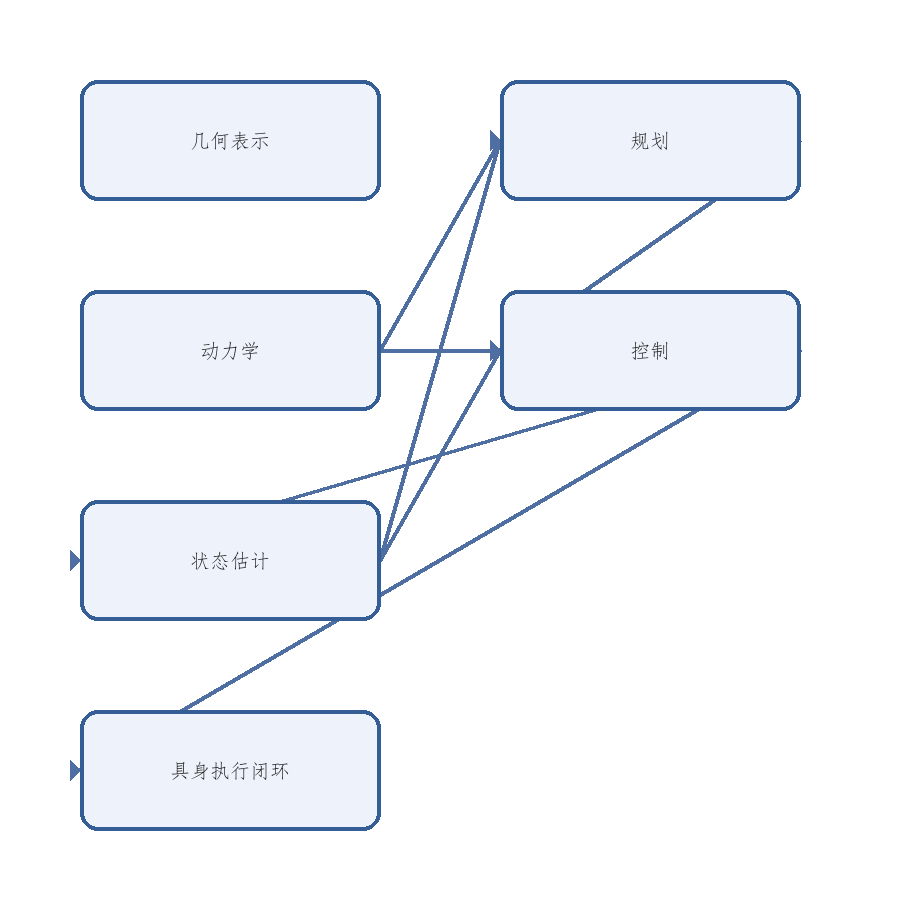
\includegraphics[width=0.9\textwidth,height=0.72\textheight,keepaspectratio]{figures/05-经典机器人学关系图.png}
\caption{05-经典机器人学关系图}
\label{fig:05-经典机器人学关系图}
\end{figure}

在当前版本中，\texttt{\detokenize{图 5-1 经典机器人学关系图}} 已承担“几何表示 - 动力学 - 规划 - 控制 - 状态估计”主关系图的职责；\texttt{\detokenize{表 5-1 经典机器人学基础与后续章节映射表}} 则把这些基础如何回流到 VLA、世界模型与部署章节正式固定下来。 本章的代码支撑重点放在两类最能代表后续具身系统接口的问题上：一类是“任务空间控制 / 阻抗控制”，用于说明高层意图如何落到可执行接触行为；另一类是 \path{EKF / 因子图状态估计}，用于说明不确定观测如何被组织成可用于控制与规划的状态变量。这样的取舍更符合本章作为基础层的职责，即用少量代表性骨架揭示核心机制，而不是把正文扩展成算法实现手册。

\section*{表 5-1 经典机器人学基础与后续章节映射表}
\addcontentsline{toc}{chapter}{表 5-1 经典机器人学基础与后续章节映射表}
\markboth{表 5-1 经典机器人学基础与后续章节映射表}{表 5-1 经典机器人学基础与后续章节映射表}

\begingroup
\small
\begin{xltabular}{\textwidth}{YYYY}
\toprule
经典基础主题 & 本章核心问题 & 在后续章节中的主要映射 & 典型关注变量 \\
\midrule
\endfirsthead
\toprule
经典基础主题 & 本章核心问题 & 在后续章节中的主要映射 & 典型关注变量 \\
\midrule
\endhead
几何表示与坐标变换 & 如何把观测、连杆、末端与环境放入统一状态空间 & 08 系统分层接口、09 感知与表征、11 VLA 输入输出接口 & 位姿、坐标系、一致性、标定误差 \\
运动学与可达性 & 某个目标在当前本体与约束下是否可执行 & 12 规划与中间表示、15 部署约束、23 场景任务分解 & 工作空间、奇异位形、逆解稳定性 \\
动力学与接触 & 执行动作时力、惯量、摩擦与冲击如何影响结果 & 10 世界模型、14 sim2real、15 硬件约束 & 质量矩阵、接触模式、摩擦、时延 \\
轨迹规划 & 如何在约束下生成可执行、可恢复的动作序列 & 12 规划推理、13 数据闭环、17 前沿专题 & 约束、平滑性、重规划代价、失败恢复 \\
闭环控制 & 如何让计划变成稳定执行，而不是离线脚本 & 11 动作表示、15 边缘部署、16 安全回退 & 带宽、稳定裕度、跟踪误差、饱和 \\
状态估计 & 如何在噪声、延迟与部分可观测下得到可信状态 & 09 多模态感知、10 内部状态、16 验证与监控 & 可观测性、协方差、漂移、同步误差 \\
建图与环境记忆 & 如何把环境结构转化为可检索、可更新的内部表示 & 07 记忆增强、10 世界模型、12 长程规划 & 拓扑、语义、时效性、可更新性 \\
约束与安全边界 & 如何给高层策略设置不可越界的物理边界 & 15 系统集成、16 安全治理、23 商业化部署 & 限幅、保护区、故障模式、接管条件 \\
\bottomrule
\end{xltabular}
\endgroup

\section*{图 5-2 接触操作的观测 - 阻抗 - 安全回退闭环}
\addcontentsline{toc}{chapter}{图 5-2 接触操作的观测 - 阻抗 - 安全回退闭环}
\markboth{图 5-2 接触操作的观测 - 阻抗 - 安全回退闭环}{图 5-2 接触操作的观测 - 阻抗 - 安全回退闭环}

\noindent\textit{源文件：\texttt{\detokenize{assets/diagrams/05-接触操作闭环图.mmd}}}
\begin{figure}[htbp]
\centering
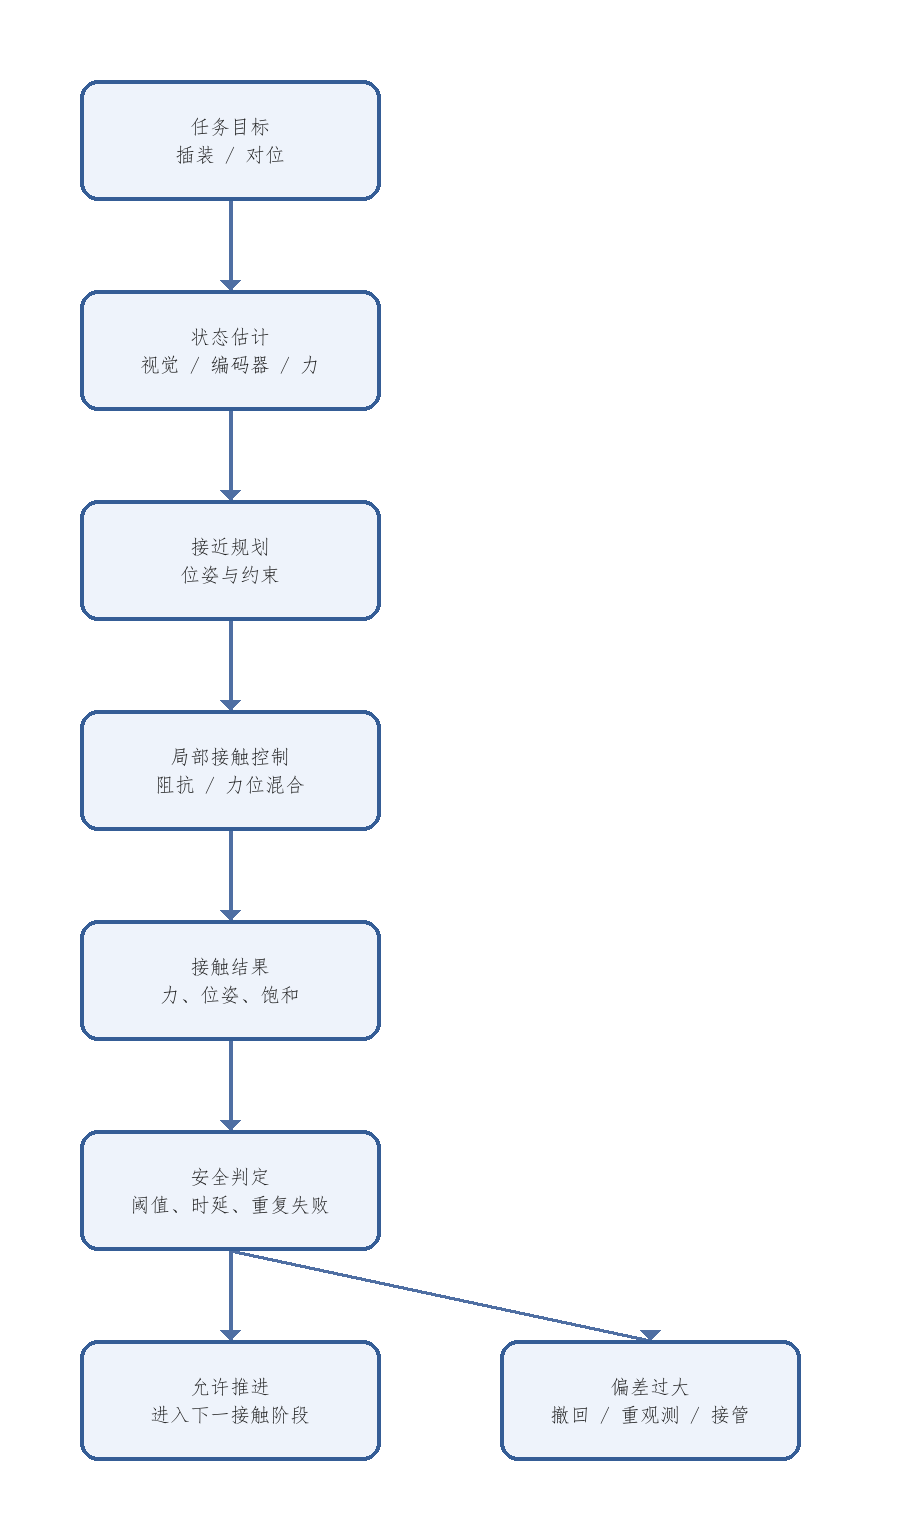
\includegraphics[width=0.9\textwidth,height=0.72\textheight,keepaspectratio]{figures/05-接触操作闭环图.png}
\caption{05-接触操作闭环图}
\label{fig:05-接触操作闭环图}
\end{figure}


\texttt{\detokenize{图 5-2}} 服务于前述柔顺插装案例：它把高层目标、状态估计、局部接触控制和安全回退分开绘制，避免把“识别到目标”误解为“已经获得可执行动作”。图中最快的安全回退通道应能绕过高层推理直接作用于局部控制；这一责任边界会在第 08、15 和 16 部分继续展开。

\section*{表 5-2 接触操作工程案例检查表}
\addcontentsline{toc}{chapter}{表 5-2 接触操作工程案例检查表}
\markboth{表 5-2 接触操作工程案例检查表}{表 5-2 接触操作工程案例检查表}

\begingroup
\small
\begin{xltabular}{\textwidth}{YYYYY}
\toprule
检查维度 & 柔顺插装中的具体问题 & 可观测证据 & 典型失效 & 推荐处理 \\
\midrule
\endfirsthead
\toprule
检查维度 & 柔顺插装中的具体问题 & 可观测证据 & 典型失效 & 推荐处理 \\
\midrule
\endhead
几何与标定 & 插头、插孔和末端坐标是否仍在同一参考系 & 重投影误差、末端位姿残差、外参版本 & 视觉定位正确但实际接触点偏移 & 重观测、标定复核、缩小接近速度 \\
接触状态 & 当前是自由运动、初触、滑动、卡滞还是已插入 & 力/力矩变化、速度下降、接触持续时间 & 把卡滞误判为正常插入 & 限力、撤回、改变接近方向 \\
局部控制 & 刚度、阻尼和位置/力通道是否与任务匹配 & 跟踪误差、接触力峰值、振荡频谱 & 刚度过高导致冲击，过低导致无法对位 & 分阶段调参、限制增益、局部搜索 \\
时间契约 & 力观测和控制命令是否仍在有效时间窗内 & 时间戳差、通信抖动、控制周期 & 过时观测驱动了新的力命令 & 丢弃过期帧、降级到保守模式 \\
安全回退 & 哪些条件必须中断自主执行 & 碰撞阈值、关节限位、重复失败计数 & 反复尝试导致过载或磨损 & 立即撤回、记录失败、请求人工接管 \\
\bottomrule
\end{xltabular}
\endgroup

\section*{代码 5-1 任务空间控制最小骨架}
\addcontentsline{toc}{chapter}{代码 5-1 任务空间控制最小骨架}
\markboth{代码 5-1 任务空间控制最小骨架}{代码 5-1 任务空间控制最小骨架}

\begin{lstlisting}[language=python]
import numpy as np

def task_space_pd(x, x_ref, J, dq, Kp, Kd):
    e = x_ref - x
    dx = J @ dq
    wrench = Kp @ e - Kd @ dx
    tau = J.T @ wrench
    return tau
\end{lstlisting}

上面的骨架只保留了一个最核心事实：高层规划最后必须通过 Jacobian、误差反馈和关节力矩映射，才能变成真实可执行的闭环命令。

% Generated from 06-学习型机器人与训练闭环基础.md; edit the LaTeX source after migration.

\part*{第六部分 学习型机器人与训练闭环基础}
\addcontentsline{toc}{part}{第六部分 学习型机器人与训练闭环基础}
\markboth{第六部分 学习型机器人与训练闭环基础}{第六部分 学习型机器人与训练闭环基础}

如果说第五部分说明了机器人为何始终受制于物理、控制与状态估计，那么本部分要回答的则是另一个同样关键的问题：一旦机器人进入学习路线，系统的主要矛盾会如何变化。传统模块化机器人往往把重点放在显式建模、手工接口和结构化工程流程上；学习型机器人则试图把其中一部分能力交给数据驱动方法学习。但这并不意味着问题被简化，相反，它通常把问题重写为另一组更难的对象：数据从哪里来、训练目标如何定义、离线与在线如何衔接、失败样本如何回流、仿真与现实如何迁移，以及系统如何在闭环中持续修正。

因此，本部分并不把模仿学习、强化学习、表示学习和 sim2real 写成互不相干的算法词条，而是把它们统一放在“训练闭环”这一主线上理解。所谓学习型机器人，真正新增的并不只是某个网络结构，而是系统开始依赖一条持续的数据-训练-部署-反馈回流链路来积累能力。也正因为此，学习型机器人既带来了前所未有的泛化可能，也引入了新的脆弱性：covariate shift、数据分布偏移、探索成本、仿真失真、训练目标错配和部署中长尾失败。

\chapter*{27. 模仿学习}
\addcontentsline{toc}{chapter}{27. 模仿学习}
\markboth{27. 模仿学习}{27. 模仿学习}

\section*{27.1 行为克隆}
\addcontentsline{toc}{section}{27.1 行为克隆}


模仿学习之所以长期是机器人学习最现实的起点，不是因为它最“先进”，而是因为它最符合现实数据获取条件。对许多操作任务、移动任务和服务任务而言，最容易拿到的数据并不是大规模在线试错样本，而是人类示教、遥操作轨迹、脚本演示或专家控制记录。行为克隆的基本思想，就是把这些示教轨迹直接转化为监督学习问题：给定观测 \(o_t\)，学习一个策略 \(\pi_\theta\) 输出动作 \(a_t\)。

最基本的训练目标通常写为：

\begingroup
\footnotesize
\begin{equation*}
\min_{\theta} \sum_{t=1}^{T} \lVert \pi_{\theta}(o_t) - a_t^\ast \rVert^2
\end{equation*}
\endgroup

其中，\(a_t^\ast\) 是专家动作。这种写法的优点在于简单直接：不需要显式奖励函数，不需要昂贵探索，也能快速建立一个“会做基本动作”的初始策略。因此，从早期视觉运动策略到今天的大量机器人示教学习系统，行为克隆一直是最自然的入口，代表性工作可参见 \href{https://arxiv.org/abs/1504.00702}{《End-to-End Training of Deep Visuomotor Policies》}。

但行为克隆最核心的脆弱性也非常清楚：训练时看到的是专家状态分布，部署时却会逐步落入策略自己诱发的状态分布。一旦出现微小误差，系统就可能越来越偏离专家轨迹，并在后续时间步中累积放大。这就是学习型机器人里最基本也最重要的 covariate shift 问题。

更形式化地说，行为克隆真正优化的是专家诱导分布上的监督风险，而部署时关心的却是策略自身诱导分布上的长期性能。若把专家分布写成 \(d^{\pi_E}(o)\)，策略分布写成 \(d^{\pi_\theta}(o)\)，则训练目标更接近：

\begingroup
\scriptsize
\begin{equation*}
\mathcal{L}_{\mathrm{BC}}(\theta)=\mathbb{E}_{(o,a^\ast)\sim d^{\pi_E}}\bigl[-\log \pi_\theta(a^\ast \mid o)\bigr]
\end{equation*}
\endgroup

但部署期真正影响成功率的却是：

\begingroup
\footnotesize
\begin{equation*}
J(\pi_\theta)=\mathbb{E}_{o\sim d^{\pi_\theta}}[\text{task success or return}]
\end{equation*}
\endgroup

这两个分布一旦分离，哪怕单步拟合误差很小，也会在闭环滚动中被反复放大。也正因为如此，后来的 DAgger、在线纠偏与失败回流路线，并不是对行为克隆的“可选增强”，而是在正面修补这一分布错位。

\section*{27.2 逆强化学习与偏好学习}
\addcontentsline{toc}{section}{27.2 逆强化学习与偏好学习}


如果把行为克隆理解为“直接模仿专家做了什么”，那么逆强化学习与偏好学习更接近于“推断专家为什么偏好这样做”。二者都试图把人类标准从动作层抬升到目标层，但处理反馈的形式不同。逆强化学习通常假设存在某个隐含奖励函数 \(r_\phi(s, a)\)，专家轨迹之所以优于其他轨迹，是因为它们在该奖励下取得了更高累计回报；偏好学习则不要求先显式恢复完整奖励，而是允许人类只对两段候选行为表达“哪一段更好”，再从成对比较中学习一个可用于排序或训练的偏好模型。

若以轨迹 \(\tau\) 表示一段状态-动作序列，偏好学习常见的最小形式可以写成：

\begingroup
\footnotesize
\begin{equation*}
P(\tau_i \succ \tau_j) = \sigma(f_\phi(\tau_i) - f_\phi(\tau_j))
\end{equation*}
\endgroup

其中 \(f_\phi(\tau)\) 可被视为轨迹奖励或质量评分器。逆强化学习则更强调从专家数据中恢复解释行为的奖励结构，而偏好学习更强调用低成本人类比较信号去拟合“什么叫更好”。对具身系统而言，这种差别很重要，因为很多高质量标准并不是单步动作正确，而是整段行为更平滑、更安全、更符合人类协作习惯。

从工程工作流看，一条典型链路通常是：策略先生成若干候选行为片段，再由人类、规则系统或高可信脚本对片段进行偏好比较，之后训练奖励/偏好模型，最后把它接到离线 RL、重排序器或在线微调回路里。其最小伪代码可以写成：

\begin{lstlisting}[language=python]
segments = collect_candidate_trajectories(policy, env)
labels = query_human_preferences(segments)
reward_model = fit_preference_model(segments, labels)
policy = optimize_policy_with_reward_model(policy, reward_model)
\end{lstlisting}

从工程角度看，逆强化学习与偏好学习的真正价值，不在于它们能神奇地自动发现完美奖励，而在于它们提供了一种把“难以直接写成公式的人类标准”逐步转译进训练目标的机制。对于服务机器人、协作机器人和家庭场景系统，这一点尤其重要，因为很多高质量行为的评价依赖软约束而不是单一成功标签。与此同时，这条路线也有明显代价：偏好标注往往昂贵、主观且受上下文影响；恢复出来的奖励未必具有强可迁移性；一旦数据分布变化，原先学到的偏好结构可能迅速失效。

当人们发现“直接模仿动作”不足以表达复杂任务目标时，就会自然走向另一条思路：不一定模仿动作本身，而是试图恢复驱动这些动作的偏好、代价或奖励结构。逆强化学习的吸引力在于，它试图回答“专家为什么这么做”，而不仅仅是“专家做了什么”。对于同一个高层目标，可能存在多条行为轨迹；若只模仿表面动作，系统容易过拟合于演示细节，而不能抓住真正应优化的任务结构。

偏好学习则进一步把这一思想推向更灵活的人类反馈接口。人类未必总能给出完整专家轨迹，但可以在候选行为之间表达“哪个更好”“哪个更安全”“哪个更自然”。这类方法在具身系统中尤其有意义，因为很多任务的高质量标准并不完全等于“到达目标状态”，还包括接触稳定性、动作平滑性、人机共处安全性和符合现场习惯的执行风格。

\section*{27.3 DAgger 与闭环纠偏}
\addcontentsline{toc}{section}{27.3 DAgger 与闭环纠偏}


DAgger 之所以在模仿学习脉络中如此关键，是因为它清楚指出：如果只在离线专家分布上训练，那么策略在部署时引发的状态偏移会持续累积，因此必须让训练过程看到策略自己会走到的状态，并由专家对这些状态重新标注动作。 其原始论文可参见 \href{https://proceedings.mlr.press/v15/ross11a.html}{DAgger：数据聚合式模仿学习}。

如果把这个思想写成最朴素的流程，就是：

\begin{enumerate}
\item 用专家数据训练初始策略
\item 让当前策略自己运行
\item 在策略实际访问到的状态上收集专家纠正动作
\item 聚合新旧数据重新训练
\end{enumerate}

这件事的重要性，不在于 DAgger 是某个必须逐字复现的算法，而在于它第一次把模仿学习明确推向了闭环训练思路。也就是说，学习型机器人不能只依赖“第一次录好的示教”，而必须把部署中的偏差重新回收到训练中。

\begin{lstlisting}[language=python]
# 示例：DAgger 风格的数据聚合骨架
dataset = initial_expert_dataset()
policy = train_policy(dataset)

for _ in range(num_rounds):
    states = rollout(policy)
    corrections = [expert_action(s) for s in states]
    dataset.extend(zip(states, corrections))
    policy = train_policy(dataset)
\end{lstlisting}

这个片段当然省略了现实中的很多细节，例如部分人工标注、失败回放筛选和安全接管机制，但它说明了一条关键主线：模仿学习一旦认真做下去，就会自然演化成训练闭环问题，而不是静态监督学习问题。

\section*{27.4 示教数据如何塑造具身能力边界}
\addcontentsline{toc}{section}{27.4 示教数据如何塑造具身能力边界}


示教数据并不只是给模型提供“正确答案”，它还在深层上塑造了系统认为哪些动作是正常的、哪些状态是常见的、哪些恢复路径是被允许的。若示教主要来自熟练操作者、固定场景和成功片段，模型学到的往往是干净、规范但覆盖面有限的行为分布；若示教包含更多失败修正、犹豫过程和边界案例，系统更可能获得现实环境中真正有用的恢复性能力。

也因此，示教数据的价值不应只按数量衡量，更应按覆盖的行为边界衡量。很多具身系统后续泛化上限，早在示教采集阶段就已经被决定了一大半。

模仿学习的真正上限，往往不由网络结构决定，而由示教数据的分布、覆盖和质量决定。系统若只见过桌面抓取，就很难自然具备移动操作能力；若只见过成功轨迹，就往往缺少失败恢复能力；若示教本身高度脚本化，则模型即使泛化也更可能泛化到脚本模式，而不是开放世界任务。因此，示教数据并不是“喂给模型的原料”那么简单，而是在很大程度上定义了系统可学会什么、学不会什么、在哪些边界最容易失败。

**工程案例：从离线示教到真机纠偏的策略闭环。** 设想一个视觉条件的抓取与放置技能：团队先用遥操作收集一批正常完成轨迹，训练行为克隆或动作序列策略；随后把候选策略限制在低风险工作区内进行短时试运行，并把抓空、对象滑动、末端错位、因遮挡而停滞等片段单独记录。这个过程的关键不是“上线后多收一点数据”，而是主动让策略进入它自己会诱发的状态分布。DAgger 的理论动机正来自这一点：在序列决策中，后续观测会受前一步动作影响，纯离线监督学习因此容易在自身造成的偏差状态上失效，参见 \href{https://proceedings.mlr.press/v15/ross11a.html}{Ross、Gordon 与 Bagnell 的 DAgger 论文}。

若第 \texttt{\detokenize{k}} 轮试运行收集到的人工纠偏样本为 \(C_k\)，一个受控的数据更新可以写成：

\begingroup
\scriptsize
\begin{equation*}
\mathcal{D}_{k+1} = \mathcal{D}_k \cup \operatorname{filter}(C_k),
\qquad \pi_{k+1} = \operatorname{train}(\mathcal{D}_{k+1})
\end{equation*}
\endgroup

这里的 \texttt{\detokenize{filter}} 不是简单删除坏数据，而应至少区分可恢复偏差、高风险事件、传感异常和标注错误。以动作扩散路线为例，\href{https://www.roboticsproceedings.org/rss19/p026.pdf}{Diffusion Policy} 将视觉条件、动作序列生成和滚动时域执行结合起来，适合说明策略可以输出一段候选动作而非单步命令；但它并不改变上述工程事实：若回流样本没有时间对齐、失败类别和上线条件，模型只会把现场噪声重新编码进策略。

一个可运行的闭环至少需要四道质量门：第一，离线保留集不仅看平均成功率，还要包含偏差状态与恢复片段；第二，仿真或影子执行检查动作是否越过已知安全边界；第三，真机以受限场景灰度运行，并保留人工接管；第四，版本更新后对旧任务做回归测试，防止局部补丁造成已部署技能退化。这个案例说明的是“训练闭环为何必要”，不能据此推出任何一种策略范式在所有任务、本体或接触条件下都更可靠。

\chapter*{28. 强化学习}
\addcontentsline{toc}{chapter}{28. 强化学习}
\markboth{28. 强化学习}{28. 强化学习}

\section*{28.1 MDP 与策略学习基础}
\addcontentsline{toc}{section}{28.1 MDP 与策略学习基础}


对机器人而言，MDP 的真正作用并不是把现实世界“简化成五元组”，而是强迫研究者明确哪些量被当作状态、哪些量被当作动作、奖励究竟偏向结果还是过程、以及策略更新究竟是在拟合什么行为因果链。很多路线争论表面看发生在算法层，实质上却是 MDP 设定不同：有的系统把恢复动作写进动作空间，有的把失败后重试外包给执行器；有的把安全作为硬约束，有的只把它当作奖励惩罚项。只要这层问题没说清，后续任何“算法更强”的比较都很容易失真。

强化学习之所以吸引机器人领域，是因为它看起来提供了一种比模仿学习更自主的能力形成机制：系统不必只复制专家，而可以通过与环境交互优化长期回报。其最经典的问题设定是马尔可夫决策过程：

\begin{equation*}
\mathcal{M} = (\mathcal{S}, \mathcal{A}, P, r, \gamma)
\end{equation*}

其中，状态 \(s_t\)、动作 \(a_t\)、转移概率 \texttt{\detokenize{P}}、奖励 \texttt{\detokenize{r}} 和折扣因子 \(\gamma\) 定义了一条长期决策问题。策略学习的目标通常写为最大化期望累计回报：

\begingroup
\footnotesize
\begin{equation*}
J(\pi) = \mathbb{E}_{\pi}\left[\sum_{t=0}^{T} \gamma^t r_t \right]
\end{equation*}
\endgroup

这一目标的吸引力在于，它允许系统为了长期任务完成度而不是单步模仿精度去优化行为。对于抓取、步态稳定、动态控制和长时程任务，强化学习因此提供了比行为克隆更自然的闭环优化视角。

\section*{28.2 在线 RL 与离线 RL}
\addcontentsline{toc}{section}{28.2 在线 RL 与离线 RL}


在线 RL 与离线 RL 的区别，不只是“是否接触环境”，而是策略更新是否持续依赖新采样数据。在线 RL 假设策略 \(\pi_\theta\) 在训练过程中不断与环境交互，采样新轨迹、估计价值、再更新策略；离线 RL 则固定在一个已经记录好的数据集 \(\mathcal{D}\) 上学习，训练期间不再假设可以无限制获得新样本。对现实机器人而言，这个区别极其关键，因为真机交互昂贵、缓慢、易损且存在安全边界。

若把两者写成最小流程，在线 RL 更像：

\begin{lstlisting}[language=python]
for step in range(K):
    trajectories = rollout(policy, env)
    critic = update_value_function(critic, trajectories)
    policy = improve_policy(policy, critic, trajectories)
\end{lstlisting}

离线 RL 则更像：

\begin{lstlisting}[language=python]
dataset = load_logged_robot_data()
for step in range(K):
    batch = sample(dataset)
    critic = update_value_function(critic, batch)
    policy = conservative_policy_improvement(policy, critic, batch)
\end{lstlisting}

这两条路线面对的问题完全不同。在线 RL 的主要挑战是探索成本、样本效率与安全约束；离线 RL 的主要挑战是分布外动作带来的价值误估。也正因如此，机器人中的离线 RL 常常不会做“自由策略改进”，而会加入保守约束，要求策略不要偏离数据分布太远。现实系统因此普遍采用“离线预训练 + 有限在线校正”的折中流程。

若把离线 RL 的核心困难进一步形式化，可以理解为：评论器 \(Q(s,a)\) 必须在只见过数据集 \(\mathcal{D}\) 的条件下，为策略可能提出的新动作给出估值。一旦对分布外动作过于乐观，策略优化就会朝着“数据里从未真正支持过”的危险区域漂移。以 Conservative Q-Learning 为代表的一类方法，会在 Bellman 误差之外显式加入“压低分布外动作价值”的保守项，典型目标可写为：

\begingroup
\scriptsize
\begin{equation*}
\min_Q \underbrace{\mathbb{E}_{(s,a,r,s')\sim\mathcal{D}}\left[\left(Q(s,a)-\mathcal{B}^{\pi}Q(s,a)\right)^2\right]}_{\text{Bellman 误差}}
+ \alpha\left(\mathbb{E}_{s\sim\mathcal{D},\,a\sim\mu(\cdot\mid s)}[Q(s,a)]-\mathbb{E}_{(s,a)\sim\mathcal{D}}[Q(s,a)]\right)
\end{equation*}
\endgroup

其中 \(\mu(\cdot\mid s)\) 表示某个更宽的候选动作分布，第二项的作用是主动降低“数据没有支撑的动作”在 \(Q\) 函数中的估值，相关代表性工作可参见 \href{https://arxiv.org/abs/2006.04779}{《Conservative Q-Learning for Offline Reinforcement Learning》}。从机器人角度看，这个保守项的意义不是让算法显得更复杂，而是把“不要在纸面上幻想一个现实里并不可靠的动作”直接写进优化目标。

但强化学习一进入真实机器人，就会立刻遭遇现实约束。在线 RL 的理想图景是系统自己在环境中反复试错，但真实机器人中的试错是昂贵的、慢的，而且可能造成磨损、碰撞或安全风险。因此，机器人领域长期非常依赖仿真环境、历史缓冲区、示教初始化和离线数据集。于是，RL 很快就分化为两条路线：一条强调直接在线交互优化，另一条强调在已有数据上做离线策略学习，再辅以有限在线修正。

这一分化本身就说明，机器人中的 RL 从来不是“让机器人自己学一切”那么简单，而是始终要在探索收益与现实代价之间做工程折中。

\section*{28.3 层级强化学习}
\addcontentsline{toc}{section}{28.3 层级强化学习}


层级强化学习可以被视作“把长时程控制问题拆成多个不同时间尺度上的决策器”。最经典的结构是高层管理器和低层执行器：高层每隔若干步产出一个子目标、技能索引或 option，低层则在更高频率上执行连续控制，努力把系统带到该子目标附近。

若把这一结构写成统一抽象，可以得到：

\begin{equation*}
g_t = \pi_H(s_t), \qquad a_t = \pi_L(s_t, g_t)
\end{equation*}

其中 \(g_t\) 是高层在慢时间尺度上给出的子目标或技能标签，\(\pi_L\) 是条件于子目标的低层策略。它们回答的是同一个问题：如何避免让单层策略同时承担“长时程意图规划”和“短时程稳定控制”两类职责。

一个极简工作流可以写成：

\begin{lstlisting}[language=python]
goal = high_level_policy(state)
for _ in range(skill_horizon):
    action = low_level_policy(state, goal)
    state, reward = env.step(action)
    if reached(goal, state):
        break
\end{lstlisting}

这个结构之所以在具身系统里格外自然，是因为真实机器人本来就具有多层时间尺度。语言指令和任务阶段往往以秒级或十秒级变化，而关节控制、接触稳定和避障修正通常是毫秒级到百毫秒级问题。层级 RL 的意义，就是试图让学习系统也尊重这种物理时间结构，而不是把所有决策都塞进同一个平面里。 层级结构的关键收益，在于它把原本难以直接优化的长时程信用分配问题拆成多个较短决策链路。高层不必在每个控制周期都重新决定末端执行器如何运动，而可以在更慢时间尺度上决定当前应激活哪类技能、追求哪个局部目标。低层则专注于在受限上下文中完成局部控制最优化。对于具身任务，这种分离通常不仅提升样本效率，也更方便插入人类先验、安全约束和程序化结构，因此它在后来的 VLA、行为树、技能图谱和程序化规划中不断以不同形式重现。

随着任务变长、状态空间变大、动作结构变复杂，单层策略很难同时处理高层子目标分解与低层连续控制。因此，层级强化学习自然出现：高层策略选择子目标或技能，低层策略负责具体执行。这条路线对具身智能后续的“技能库”“大小脑分层”“程序化中间表示”极具启发性，因为它说明学习系统也会自然走向分层，而不是无限维持单一平面策略。

\section*{28.4 安全强化学习}
\addcontentsline{toc}{section}{28.4 安全强化学习}


安全强化学习之所以在机器人里必须单列，是因为传统 RL 默认的“多试错、多探索”在真实系统中成本极高。机器人每一次危险动作都可能对应硬件损伤、人身风险、现场停线或数据污染，因此安全不能只作为奖励函数里的一项惩罚项，而往往要进入约束、屏障、动作裁剪和人类接管机制中。

这也意味着，机器人中的安全 RL 更像是“在可接受风险边界内学习”，而不是“先任意学习、后再部署”。很多看似降低探索自由度的安全机制，恰恰是让真实学习能够持续进行的必要前提。 这一点之所以需要单独强调，是因为不少关于 RL 的乐观叙事默认了“只要探索足够多，策略总会变好”。但在真实机器人里，不安全探索不仅意味着训练成本增加，还可能直接损坏设备、破坏环境或伤及人员。因此，安全 RL 在具身场景中更像是一套训练制度，而非单一算法名词。它要求我们同时设计奖励、约束、监控、回退和人工接管机制，并承认某些状态区域根本不允许被自由探索。

机器人中的 RL 还必须面对一个纯软件智能体不那么尖锐的问题：探索本身可能带来真实物理风险。因此，安全强化学习并不是附属分支，而几乎是机器人 RL 的默认前提。很多现实系统不得不通过动作裁剪、约束优化、shielding、风险敏感回报和人类接管来限制探索空间，否则训练过程本身就会不可接受。

若把这一问题写成更标准的受约束优化形式，机器人里的安全 RL 往往更接近 constrained MDP，而不是普通 MDP：

\begingroup
\footnotesize
\begin{equation*}
\max_{\pi} J_r(\pi)
\quad \text{s.t.} \quad
J_c(\pi) \le d
\end{equation*}
\endgroup

其中 \(J_r(\pi)\) 表示任务回报，\(J_c(\pi)\) 表示碰撞、超力矩、越界、温升或人机接近风险之类的成本累计，\(d\) 表示允许上界。其拉格朗日形式可写成：

\begingroup
\footnotesize
\begin{equation*}
\mathcal{L}(\pi,\lambda)=J_r(\pi)-\lambda\bigl(J_c(\pi)-d\bigr), \qquad \lambda \ge 0
\end{equation*}
\endgroup

这类写法的重要性在于，它把“安全不是偏好，而是硬边界”明确进了问题定义。像 \href{https://arxiv.org/abs/1705.10528}{《Constrained Policy Optimization》} 这样的工作之所以长期被反复引用，不只是因为它提供了一个算法名字，而是因为它把“每次更新都不能把系统推到明显更危险的区域”这一工程直觉，转写成了可分析、可实现的策略更新约束。对真实机器人而言，shielding、动作裁剪、工作空间屏蔽和安全接管，很多都可以视为这个 constrained MDP 视角在系统层的工程展开。

\section*{28.5 为什么 RL 在机器人里既重要又常被高估}
\addcontentsline{toc}{section}{28.5 为什么 RL 在机器人里既重要又常被高估}


RL 之所以重要，是因为它为机器人提供了一种超越纯示教模仿的路径，使系统能够通过交互优化长期回报、探索策略改进空间并在某些接触与顺序任务上学到人类示教之外的行为结构。尤其在仿真中，RL 仍是许多控制技能与策略优化工作的核心工具。

但 RL 又常被高估，是因为它在论文与视频里常常代表能力上限，而在真实部署中却很难单独承担整套系统能力。真实世界中的数据效率、探索风险、分布漂移、维护成本和奖励设计难题，都使得 RL 更适合作为系统中的一层能力来源，而不是总被浪漫化为万能学习范式。

强化学习在机器人中的真实价值，主要体现在它能够对闭环行为进行长期优化，尤其适合那些难以手工设计控制器、但又可以通过回报近似描述目标的任务。\href{https://arxiv.org/abs/1806.10293}{QT-Opt} 的意义正在于此：它并不是证明“机器人会自己学一切”，而是说明当真实交互数据规模足够大时，闭环 RL 可以在抓取这类具体任务上显著提高鲁棒性与恢复能力。

但 RL 也经常被高估。原因并不神秘：奖励设计困难、探索代价高、样本效率低、真实世界训练慢、安全风险高。这意味着 RL 在机器人里更常扮演“局部行为优化器”或“特定子系统能力增强器”的角色，而不是一个能天然吞掉全部系统问题的统一方案。

\chapter*{29. 表示学习与多任务学习}
\addcontentsline{toc}{chapter}{29. 表示学习与多任务学习}
\markboth{29. 表示学习与多任务学习}{29. 表示学习与多任务学习}

\section*{29.1 自监督表示学习}
\addcontentsline{toc}{section}{29.1 自监督表示学习}


自监督表示学习之所以在机器人中重要，是因为真实交互数据昂贵、标注稀缺，而系统却需要从海量未标注轨迹中先学到可压缩、可迁移、可预测的结构。相比直接端到端监督训练，自监督方法更像是在为后续控制、规划与跨任务迁移铺设共同底座。

不过，机器人里的自监督并不能简单照搬纯视觉领域经验。对具身系统而言，有用的表示不仅要“对图像变化敏感”，还要对动作后果、接触状态、对象可操作性和时序连续性敏感。否则，表示也许很适合分类或检索，却未必足够适合驱动决策。

一旦机器人不再只做单一任务，问题就不再只是“当前策略会不会做这件事”，而变成“系统能否从观测中学到跨任务可复用的结构”。这正是表示学习进入机器人主线的原因。自监督学习的吸引力在于，它允许系统在不依赖昂贵逐步标注的情况下，从多模态观测、时序结构和环境互动中学到对后续任务有用的内部表征。

从更长的脉络看，后来的多模态基础模型、VLA 和机器人 foundation models，本质上都建立在一个前提上：系统必须先学会形成比单任务监督标签更稳定、更可迁移的内部状态结构。

这也是为什么本章要把表示学习放在基础模型之前讲。它并不是附属预备知识，而是后续一切“统一接口”“多任务共享”“跨平台迁移”叙事能够成立的前置条件。

\section*{29.2 多任务共享表征}
\addcontentsline{toc}{section}{29.2 多任务共享表征}


多任务共享表征的核心问题，不是“把所有任务放在一起训练”，而是“哪些表征应该共享，哪些表征必须保留任务特异性”。一个典型架构是共享编码器加条件化任务头：视觉、触觉或状态输入先经过共享 backbone 提取通用特征，再由任务 ID、语言指令或上下文变量进行条件化，最后输出不同任务所需的动作、价值或中间状态。

其最小架构可以写成：

\begin{equation*}
z = f_\theta(o), \qquad a = \pi_\psi(z, c)
\end{equation*}

其中 \(o\) 是观测，\(f_\theta\) 是跨任务共享的表征网络，\(c\) 是任务条件，\(\pi_\psi\) 则是条件策略头。若进一步拆开，还可以为不同任务保留不同 heads：

\begin{lstlisting}[language=python]
features = encoder(obs)
action = task_head[task_id](features)
\end{lstlisting}

这类设计之所以重要，是因为机器人中大量任务共享底层结构。例如相机视角、几何约束、物体边界、抓取前的接近动作、接触前的减速策略，往往都可被多个任务复用。如果每个任务都从零训练一个独立表示，数据利用率会非常低；但如果一味强行共享，又会出现任务冲突、负迁移和梯度干扰。

如果每个任务都单独训练一个策略，那么机器人就仍然停留在“很多孤立技能拼接”的阶段。多任务学习的重要性，在于它尝试让多个任务共享一部分表示空间、技能结构和条件化接口。这样做的收益是明显的：样本可以跨任务复用，表征可以更稳定，系统也更容易在新任务上做迁移。

但代价同样明显：任务冲突、梯度干扰、表示坍塌和任务不平衡会迅速出现。因此，多任务共享并不是“任务越多越好”，而是要求系统明确哪些层应该共享、哪些层必须保留任务特异性。

\section*{29.3 通用技能库与技能迁移}
\addcontentsline{toc}{section}{29.3 通用技能库与技能迁移}


因此，技能迁移真正困难的并不是把一个名字复用到另一台机器人，而是保持其前置条件、可观测状态和失败恢复逻辑也能迁移。一个“抓取”技能在双指夹爪、五指灵巧手和吸盘末端之间，表面任务相同，内部却可能依赖完全不同的接触判据与恢复动作。这也是为什么后续很多基础模型路线会强调技能标记、动作块、可调用接口或程序式接口：它们试图把技能从纯轨迹片段提升为“带契约的中层能力对象”，从而让迁移问题变成接口重绑定，而不只是参数复制。 技能迁移的难点在于，一个看似相同的技能在不同本体、不同夹爪、不同摩擦条件和不同任务容错要求下，往往并不等价。也就是说，技能库不是静态的“动作函数仓库”，而更像一组带有适用前提、参数接口和失败模式描述的中层能力对象。后续很多基础模型路线之所以强调技能标记、动作块或程序式接口，本质上都是在寻找一种既保留可学习性、又维持技能可迁移性的中间表示。

当多任务学习进一步发展，就会自然引出“技能库”思想：与其让高层每次都直接输出低层控制，不如先学习一组可复用技能，再由高层按任务调用。这个想法对后文理解 VLA、程序化中间表示和大小脑架构都非常关键，因为现代具身系统常常不是端到端地每次都从头生成所有动作，而是试图在更稳定的技能原语之上组织行为。

从系统角度看，技能库真正提供的是一种中层可复用性。它让系统既不必把一切写死成传统程序，也不必让每次执行都从原始动作开始重新生成，因此是很多现实路线在“可学习性”和“可部署性”之间取得平衡的关键中介。

\section*{29.4 表征学习如何成为后续基础模型的前置条件}
\addcontentsline{toc}{section}{29.4 表征学习如何成为后续基础模型的前置条件}


更一般地说，基础模型之所以能够在机器人中成立，一个前提就是系统已经学会把不同任务、模态和时间尺度的信息压进某种共享表征空间。没有这一步，所谓“大模型统一一切”往往只会停留在输入输出层面的拼接，而无法形成真正可复用的内部结构。因此，把表示学习看成后续基础模型的前史，不只是历史梳理，更是在提醒我们：如果表征层设计得不对，后面再大的模型也可能只是把系统问题放大而不是解决。

Decision Transformer 的重要性，并不只在于它把强化学习（RL）重写成序列建模，而在于它表明：一旦系统开始把轨迹、回报、状态和动作放到统一序列接口中，传统策略学习与更一般的表示学习之间的边界会开始模糊，相关论文可参见 \href{https://arxiv.org/abs/2106.01345}{《Decision Transformer》}。这为后来的 VLA、动作 token 化和多模态统一接口提供了认知上的桥梁。换言之，机器人基础模型并不是凭空出现的，它们依赖的正是此前这些跨任务表示与统一接口思路的持续积累。

\chapter*{30. sim2real 与域适应}
\addcontentsline{toc}{chapter}{30. sim2real 与域适应}
\markboth{30. sim2real 与域适应}{30. sim2real 与域适应}

\section*{30.1 仿真训练的价值}
\addcontentsline{toc}{section}{30.1 仿真训练的价值}


仿真训练的真正价值，并不只是“便宜地多跑实验”，而是在真实硬件成本过高、危险动作不可直接尝试、长尾扰动难以系统组织时，提供一个可控、可重复、可批量扩展的策略形成环境。它让很多本来在真机上难以系统比较的方案，能够先在统一条件下做初筛和快速迭代。

但仿真最有价值的地方，也恰恰要求研究者对其边界保持清醒。仿真不是现实替身，而更像现实前的训练场和过滤器。若把它当作直接等价的能力证明，就会高估策略的真实部署成熟度；若把它当作结构化筛选工具，其价值则非常高。 从研究方法论上看，仿真还承担着“解耦问题”的作用。真实系统中的失败常常由多种因素叠加导致，而在仿真环境中，研究者可以更系统地单独操纵视觉纹理、动力学参数、接触模型、控制延迟和任务扰动，从而辨识究竟是哪一层假设在失效。也正因如此，仿真不是廉价替代品，而是一种结构化实验平台。后续像 NVIDIA Isaac、MuJoCo、Omniverse、Habitat 这类基础设施的重要性，不仅在于“能跑更多实验”，更在于它们塑造了问题被提出和被验证的方式。

只要真实机器人训练成本高、速度慢、风险大，仿真就几乎不可避免。仿真最大的价值，并不是“替代现实”，而是提供一种可大规模、可并行、可控制、可重复的试验环境，使系统能够在其中学习基础行为、验证训练目标和提前暴露明显失效模式。

对这份报告来说，仿真章节的重要作用还在于建立一个判断习惯：凡是仿真结果，都应继续追问它究竟证明了“结构有效”还是“部署可行”。把这两者分开，后续解读很多论文时会稳得多。

\section*{30.2 域随机化与域自适应}
\addcontentsline{toc}{section}{30.2 域随机化与域自适应}


更稳妥的理解方式是把二者看成两种互补策略。域随机化是在训练期主动扩大输入和动力学分布，让策略学会对变化不敏感；域自适应则是在部署前或部署中显式估计“我现在身处哪个域”，并对表征或参数做针对性修正。前者偏向保守覆盖，后者偏向定向补偿。对具身系统而言，很多成功方案并不是二选一，而是先用域随机化获得基础鲁棒性，再用少量真机数据或在线校准做末端收敛，这比单独押注某一条路线更符合现实工程。 域随机化的思想，是主动让训练分布比目标部署分布更“宽”，以换取策略对未见扰动的容忍度；域自适应则更强调学习如何桥接仿真与真实观测之间的表征差异。两者都不是银弹。随机化过弱，泛化无效；随机化过强，策略可能学不到任何稳定结构。自适应若只对视觉层有效，而真实失配主要来自接触动力学和控制延迟，也难以真正解决问题。因此，sim2real 的关键不是套用某个名词，而是识别系统究竟在哪一层发生了跨域断裂。

但仿真与现实之间从来不存在天然无缝映射。视觉纹理、光照、接触摩擦、执行器延迟、传感器噪声、对象分布和环境扰动都可能发生偏移。因此，sim2real 路线通常需要通过域随机化、域自适应、系统辨识和现实微调来缩小差距。

这里最重要的理解是：sim2real 并不是部署前最后做的一步“小修补”，而是一条贯穿训练早期设计的结构性问题。你在仿真中如何定义任务、如何选状态、如何建奖励、如何建动力学，都会直接影响后续现实部署是否还能成立。

也就是说，sim2real 成败往往早在“问题怎么被表述”这一层就埋下了种子，而不是只在最后迁移那一刻才出现。后文再谈世界模型、基础模型和部署时，都应保留这一视角。

\section*{30.3 现实部署中的失效模式}
\addcontentsline{toc}{section}{30.3 现实部署中的失效模式}


现实部署中的失效模式，往往并不是模型“完全不会做任务”，而是系统在长时程、弱扰动累积和异常边界条件下逐渐暴露脆弱性。例如感知偏移导致抓取点慢慢漂移、策略对某类照明特别敏感、恢复动作在少数边角状态下不可用、或上层计划在连续小误差后失去一致性。

这些失效模式之所以重要，是因为它们更接近真正的运维成本来源。很多系统不是败在第一次任务，而是败在第十次、第一百次和跨场景重复后。理解失效模式，比只关注平均成功率更接近真实部署质量。 从部署复盘角度看，失败模式分析应尽量落到可归责的系统层级。例如，抓取失败究竟是检测框飘移、深度估计偏差、抓取位姿候选错误、接触模型不准，还是末端执行器闭合延迟过大？如果没有这种分层归因，团队就容易把所有失败都模糊归结为“模型泛化不够”，从而错过真正的系统瓶颈。后续报告在评价企业 demo 或学术结果时，也应尽量用这种失效模式框架来判断其工程含金量。

现实中的失效往往不是单点误差，而是多种偏移叠加：视觉模型在新光照下变差，接触模型与真实摩擦失配，控制时延导致原本稳定的轨迹开始振荡，状态估计漂移让策略输入逐步失真。也正因为此，“仿真里会做”从来不能自动推出“现实里能稳定做”。

这类失效模式也说明，部署分析必须尽量落到分层归因，而不是笼统归因为“模型不够泛化”。只有这样，团队才可能知道应该补数据、换接口、加回退，还是重做本体与控制链路。

\section*{30.4 为什么“学得好”不等于“落得下去”}
\addcontentsline{toc}{section}{30.4 为什么“学得好”不等于“落得下去”}


“学得好”与“落得下去”之间的差距，通常不在离线指标本身，而在系统是否能承受真实部署中的分布漂移、执行误差、延迟、异常恢复和维护负担。一个策略在干净数据集、固定起始条件和可控环境中取得高成功率，并不意味着它在连续值班、复杂照明、器件老化或混杂人机协作条件下还能保持稳定表现。

从工程角度看，能否落地更像是在问：模型是否具备足够的恢复能力、是否允许人类低成本接管、是否能通过日志回流形成再训练闭环、以及其错误是否以可管理方式暴露。也正因此，学习系统的真正成熟，往往不是体现在最优片段更惊艳，而是体现在平均运行更稳、失败模式更清晰、维护流程更可复制。

这一定义会贯穿后文对企业和商业化的判断。很多路线不是“不会做”，而是“做了但还不值得交付”；两者差别不在 demo，而在恢复、维护、接管和回流是否成体系。

这一节对全书最重要的意义，在于它提前建立一个判断纪律：学习指标的提升、仿真成绩的提升、离线验证的提升，都不自动等于真实部署能力的提升。后文无论写 VLA、世界模型还是企业 demo，都必须不断回到这一点上检验。

\chapter*{31. 世界模型思想的早期来源}
\addcontentsline{toc}{chapter}{31. 世界模型思想的早期来源}
\markboth{31. 世界模型思想的早期来源}{31. 世界模型思想的早期来源}

\section*{31.1 model-based RL}
\addcontentsline{toc}{section}{31.1 model-based RL}


从算法结构上看，model-based RL 至少包含三个部件：环境模型、规划或想象模块，以及策略/价值更新模块。环境模型试图学习从当前状态和动作到下一状态及奖励的转移关系；规划模块利用该模型在内部试探多个动作后果；策略模块再根据这些“想象经验”或规划结果更新行为。

若以学习得到的动力学模型 \( \hat{P}_\phi(s_{t+1}\mid s_t,a_t) \) 和学习得到的奖励模型 \( \hat{r}_\phi(s_t,a_t) \) 表示环境模型，则最小流程可以写成：

\begin{lstlisting}[language=python]
model = fit_dynamics(real_transitions)
for state in sampled_states:
    imagined_rollouts = rollout_in_model(model, state, candidate_actions)
    score = evaluate(imagined_rollouts)
policy = improve_policy(policy, score)
\end{lstlisting}

这里真正的分水岭，不是“有没有模型”，而是模型在控制链中承担什么角色。有些系统只把模型用于生成辅助训练数据；有些把它用于候选动作排序；有些则把它直接嵌入 MPC 式在线规划。角色不同，对模型精度、稳定性和时延的要求也完全不同。 这一传统的重要性在于，它重新把“预测环境会怎样变化”放回了决策核心。与纯 model-free 路线相比，model-based RL 试图让系统通过内部推演减少真实试错需求，并在规划时显式利用未来状态结构。对于机器人而言，这一点尤其诱人，因为真实交互昂贵而危险；但也正因为如此，任何动力学建模误差都可能被规划过程放大，导致系统在内部想象中看似合理、在现实中却迅速偏离。

从控制视角看，model-based RL 的最大诱惑与最大风险恰好是同一件事：它允许系统把“少量真实样本”扩展成“大量内部推演样本”。如果把模型下的预测回报记为 \(\hat{J}(\pi)\)，真实环境回报记为 \(J(\pi)\)，那么问题的关键不只是让 \(\hat{J}\) 尽量大，而是让 \(|\hat{J}(\pi)-J(\pi)|\) 在候选动作之间保持可控。换句话说，机器人真正需要的不是一套会做漂亮想象的模型，而是一套在比较两个动作序列时，其误差不会把排序彻底颠倒的模型。

世界模型路线之所以值得单独讨论，不是因为它是近两年的新潮名词，而是因为它延续的是更早的 model-based RL 思想：系统不仅学策略，还学习环境动力学或潜在状态演化，再利用这些内部模型进行规划、想象 rollout 或策略优化。

\section*{31.2 潜空间动力学模型}
\addcontentsline{toc}{section}{31.2 潜空间动力学模型}


潜空间动力学模型的标准工作流，通常分为“编码”“潜空间转移”“解码或读出”三步。系统先用编码器把高维观测 \(o_t\) 压缩为潜变量 \(z_t\)，再在潜空间学习转移关系 \(z_{t+1}=f(z_t,a_t)\)，最后按需要解码回观测、奖励、接触属性或价值信号。它与直接像素预测的根本区别在于：模型不再试图重建全部视觉细节，而是希望保留与控制相关的最小充分结构。

一个极简架构可以写成：

\begingroup
\scriptsize
\begin{equation*}
z_t = e_\theta(o_t), \qquad \hat{z}_{t+1} = f_\phi(z_t, a_t), \qquad \hat{o}_{t+1} = d_\psi(\hat{z}_{t+1})
\end{equation*}
\endgroup

如果只关心控制而非重建，最后一步甚至不必显式解码成像素，而可以直接预测奖励、终止标志、接触模式或可供性。也正因为如此，潜空间模型常被进一步区分为“重建导向”和“控制导向”两类：前者更在意观测保真，后者更在意潜变量是否可用于规划、值函数估计和技能切换。 潜空间动力学模型的真正挑战，不只是压缩得足够小，而是要保留对决策真正重要的可控结构。若潜变量只对重建像素有利、却丢失了接触可行性、可达性或物体交互关系，那么它对机器人规划价值有限。反过来，如果潜空间过于任务特化，又会削弱跨任务复用和长期泛化能力。因此，这一层始终处在“表征压缩”与“控制充分性”之间的张力之中，这也是后续世界模型与具身基础模型路线不断分化的根本原因之一。

更严格地说，潜变量 \(z_t\) 的价值不在于“压得够小”，而在于它是否近似构成后续决策所需的充分统计量。一个更接近系统分析的要求是：

\begingroup
\footnotesize
\begin{equation*}
p(o_{t+1}, r_t, c_t \mid h_t, a_t) \approx p(o_{t+1}, r_t, c_t \mid z_t, a_t)
\end{equation*}
\endgroup

其中 \(h_t\) 表示完整历史，\(c_t\) 可以表示接触、终止或约束事件。若这个近似不成立，说明潜变量虽然便于重建，却不足以支撑控制；反之，若它能在较小维度上保留对奖励、接触和可达性的关键条件信息，它才真正有资格成为后续规划与策略优化的工作空间。

一旦观测空间变得高维，直接在像素或原始传感空间中做预测往往代价太高，于是研究者开始学习潜空间表示，并在潜空间中建模动力学。这一步非常关键，因为它把“世界模型”从简单的环境近似，推进成一种“可预测、可规划、可压缩”的内部状态结构。

\section*{31.3 想象 rollout 与规划接口}
\addcontentsline{toc}{section}{31.3 想象 rollout 与规划接口}


“想象 rollout”并不等于简单生成未来画面，它更像是在内部模型中展开一串假设动作，然后把结果交给某种决策接口消费。这个接口可以是动作重排序器、MPC 规划器、价值评估器，或者仅仅是训练时的辅助数据生成器。理解 rollout 的关键，不在于它能否看起来像未来，而在于它与下游控制器之间如何闭环。

最小的 imagination planning 过程可以写成：

\begin{lstlisting}[language=python]
for action_seq in candidate_action_sequences:
    latent = encode(obs)
    returns = 0
    for action in action_seq:
        latent, reward = model.step(latent, action)
        returns += reward
    score[action_seq] = returns
best = argmax(score)
execute(best[0])
\end{lstlisting}

这里可以看出，rollout 的核心是“候选动作序列在模型内的相对排序”，而不是必须得到完美像素视频。对机器人而言，只要内部推演足够帮助区分“更可能成功”和“更可能碰撞或失稳”的候选行为，它就可能有实际价值。 因此，想象 rollout 真正需要回答的问题，不是“能不能生成未来”，而是“生成出来的未来如何以受控方式进入决策接口”。有的系统把它用于价值评估，有的用于动作筛选，有的用于候选计划排序，还有的仅用于离线表征学习。接口不同，世界模型承担的责任也不同。把这一点说清楚很重要，因为它直接决定了我们后文评价世界模型路线时，是把它看成控制器、规划器、数据生成器，还是训练辅助器。

在真实机器人里，这个“受控方式”往往还必须把模型不确定性一并写进去。一个更贴近工程的候选序列评分常写成风险惩罚形式：

\begingroup
\scriptsize
\begin{equation*}
\mathrm{Score}(a_{t:t+H})=
\sum_{\tau=t}^{t+H}\hat{r}_\tau
-\beta \sum_{\tau=t}^{t+H}\mathrm{Uncertainty}(\hat{z}_{\tau})
\end{equation*}
\endgroup

其中第二项并不是锦上添花，而是在提醒系统：内部想象越往长时程展开，模型偏差越可能把“看起来最优”的序列推向现实中的危险区域。也正因为如此，许多世界模型系统真正可用的部分，不是把 rollout 拉得无限长，而是知道在哪个 horizon 截断、在哪些状态拒绝继续相信模型、以及何时把控制权交还给更保守的局部控制器。

\href{https://arxiv.org/abs/1803.10122}{World Models} 与 \href{https://arxiv.org/abs/1912.01603}{Dreamer} 之类工作的重要性，就在于它们明确展示了系统可以在内部模型中做想象 rollout，再据此学习策略或评估未来。对机器人来说，这一思想特别诱人，因为真实试错昂贵，而内部想象似乎提供了一种更高样本效率的替代路径。

但这里也埋下了后文世界模型章节必须正面处理的问题：生成看起来合理的未来，并不等于预测在物理上真实可执行的未来；内部模型可以帮助训练，却不自动保证部署中的稳定性与安全性。

\section*{31.4 为什么世界模型不是凭空冒出来的新潮名词}
\addcontentsline{toc}{section}{31.4 为什么世界模型不是凭空冒出来的新潮名词}


世界模型之所以看上去像一个近年流行的新词，更多是因为它在大模型与生成模型浪潮中重新获得了关注，而不是因为它在机器人与控制中毫无前史。其核心问题始终都在：系统能否通过内部模型预测环境演化、评估动作后果并在执行前进行某种形式的想象式试错。

从这个意义上说，今天的视频世界模型、潜空间 rollout、抽象预测和旧时代的模型预测控制、状态转移建模并不是彼此割裂的宇宙，而是共享同一问题核的不同技术表达。理解这一连续性，有助于避免把许多老问题仅仅因为名字更新就误判为“全新范式”。

因此，本节最重要的作用，是把世界模型重新接回学习型机器人主线。后文如果直接从生成视频或具身基础模型角度谈世界模型，很容易让它显得像一个突然冒出来的新范式；而放回这里看，它其实是基于模型的强化学习、潜空间动力学和想象式规划的继续发展，只是在模型规模和表示能力上被重新放大了。

把这一连续性看清楚，有助于我们避免被术语更新反复带偏。很多今天看似崭新的路线，真正的新意未必在问题本身，而在表示能力、数据规模和接口组织方式上。

\chapter*{本部分小结}
\addcontentsline{toc}{chapter}{本部分小结}
\markboth{本部分小结}{本部分小结}

学习型机器人真正改变的，并不是“机器人开始用神经网络了”这么简单，而是系统能力开始依赖一条持续的训练闭环：示教、交互、反馈、回流、迁移和再训练共同决定系统上限。模仿学习提供现实起点，强化学习提供闭环优化机制，表示学习提供跨任务结构，sim2real 暴露部署断裂，世界模型则尝试把环境动力学重新引入学习链路。

也正因此，本部分与后文的接口非常明确：

\begin{enumerate}
\item 与第 07 部分的接口：表示学习、序列建模和统一接口为大模型进入机器人打基础
\item 与第 10 部分的接口：世界模型并非新概念，而是这里的继续展开
\item 与第 11、13、14 部分的接口：VLA、数据工程、仿真基础设施都建立在这里的训练闭环视角之上
\item 与第 15、16 部分的接口：学习系统的最终价值仍取决于部署约束与安全条件
\end{enumerate}

\chapter*{图表与代码补充}
\addcontentsline{toc}{chapter}{图表与代码补充}
\markboth{图表与代码补充}{图表与代码补充}

本章真正值得反复回看的，不只是单个算法定义，而是它们在训练闭环中的位置关系。若把行为克隆、偏好学习、在线/离线 RL、sim2real 和世界模型放进同一张图里，会更容易看出它们并不是彼此替代的平行名词，而是在回答“数据从哪里来、目标如何定义、策略如何更新、部署偏差如何回流”这几类不同问题。

因此，后续版本中本章的图表应服务于两个稳定目标：第一，把“模仿学习 - RL - 表征学习 - 世界模型”的历史关系画清楚；第二，把“采集 - 训练 - 部署 - 失败回流”的工程闭环画清楚。与其把这些图当作装饰，不如把它们看成本章的结构索引，因为训练型机器人真正新增的就是这条长期数据与能力共演化链路。

代码层面，本章最值得保留的不是大段实现细节，而是几类最小骨架：行为克隆训练循环、离线 RL 的保守更新结构、以及 model rollout 的内部评估回路。它们能帮助读者把抽象术语重新压回到“数据如何进入优化器、优化器如何影响策略、策略又如何回到部署现场”这一条可执行链路上。

\chapter*{图 6-1 学习路线与训练闭环演化图}
\addcontentsline{toc}{chapter}{图 6-1 学习路线与训练闭环演化图}
\markboth{图 6-1 学习路线与训练闭环演化图}{图 6-1 学习路线与训练闭环演化图}

\noindent\textit{源文件：\texttt{\detokenize{assets/diagrams/06-训练闭环演化图.mmd}}}

\begin{figure}[htbp]
\centering
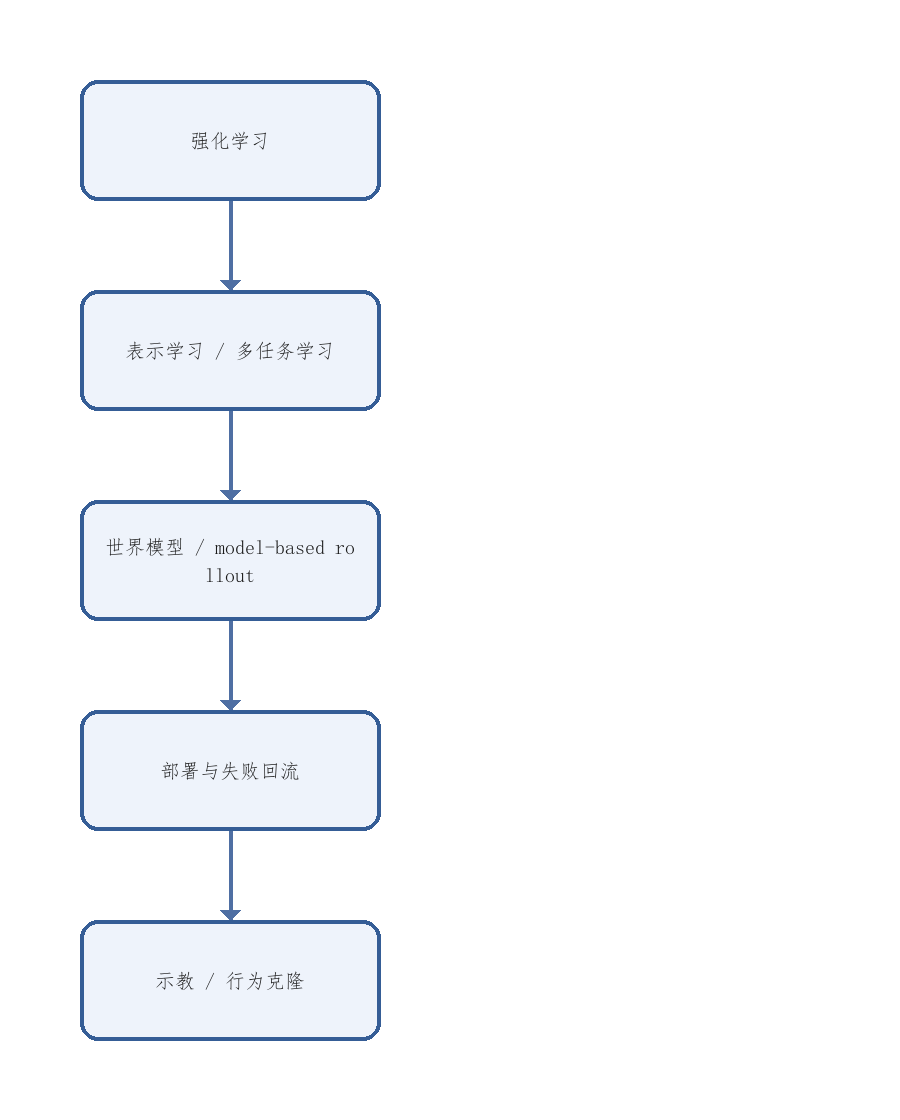
\includegraphics[width=0.9\textwidth,height=0.72\textheight,keepaspectratio]{figures/06-训练闭环演化图.png}
\caption{06-训练闭环演化图}
\label{fig:06-训练闭环演化图}
\end{figure}

\texttt{\detokenize{图 6-1 学习路线与训练闭环演化图}} 的意义，在于把两条经常被分开叙述的主线重新并到一起：一条是“模仿学习 - 强化学习 - 表示学习 - 世界模型”的能力演化主线，另一条是“数据采集 - 训练 - 部署 - 回流”的工程闭环主线。前者解释算法范式如何变化，后者解释这些范式为何会在真实机器人系统中表现出不同的可扩展性；只有把两者放在同一张图里，读者才更容易理解为什么某些训练路线在论文上成立，却在部署上成本极高。

\chapter*{图 6-2 示教策略的闭环纠偏与版本放行}
\addcontentsline{toc}{chapter}{图 6-2 示教策略的闭环纠偏与版本放行}
\markboth{图 6-2 示教策略的闭环纠偏与版本放行}{图 6-2 示教策略的闭环纠偏与版本放行}

\noindent\textit{源文件：\texttt{\detokenize{assets/diagrams/06-闭环纠偏与版本放行图.mmd}}}
\begin{figure}[htbp]
\centering
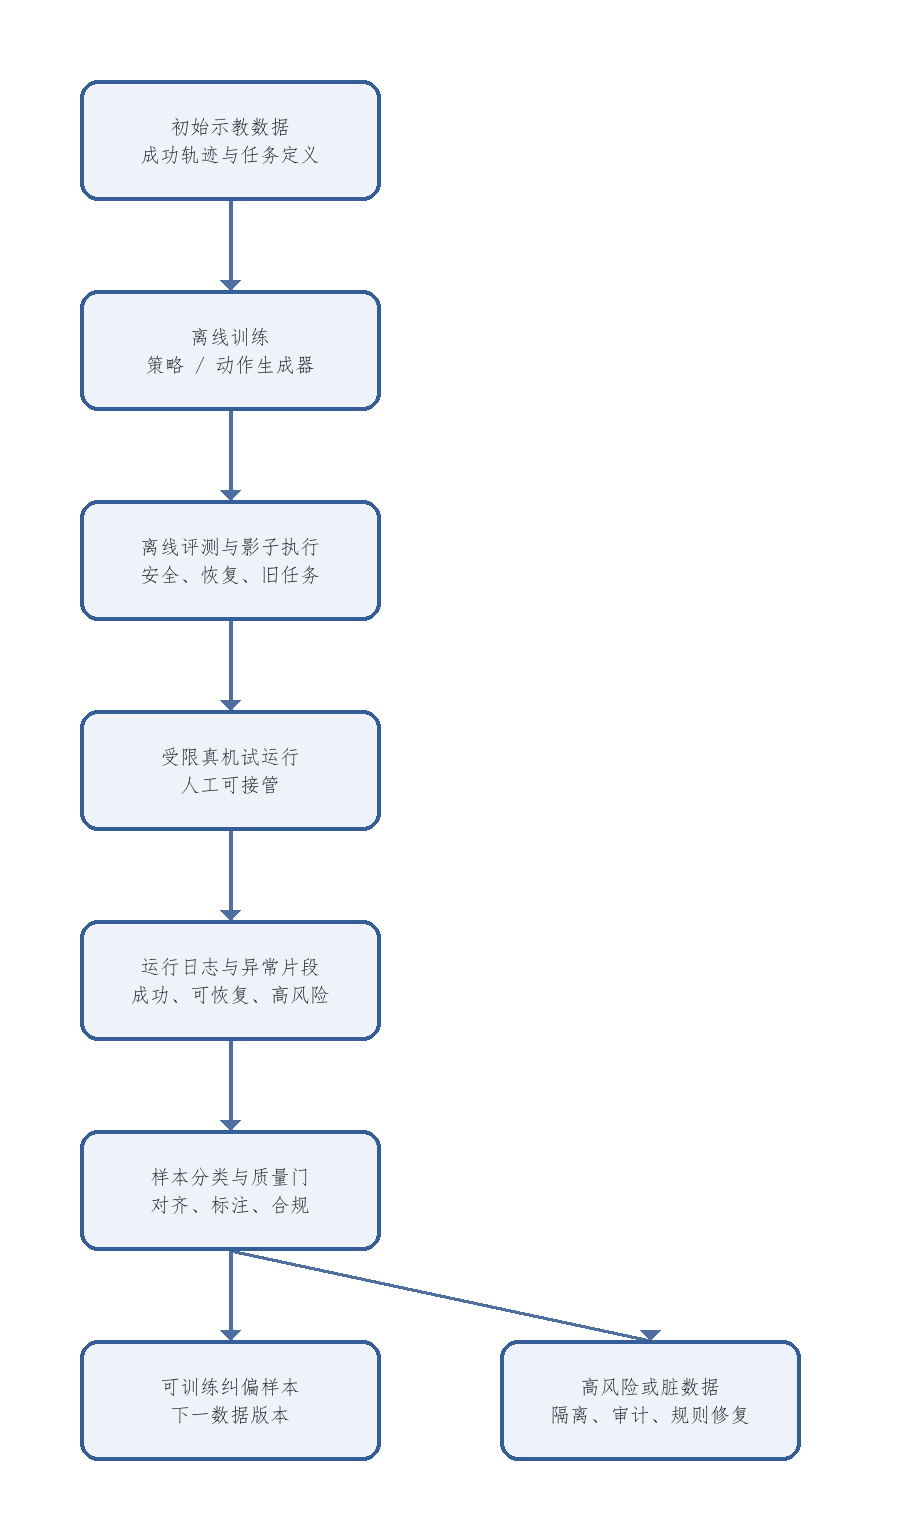
\includegraphics[width=0.9\textwidth,height=0.72\textheight,keepaspectratio]{figures/06-闭环纠偏与版本放行图.png}
\caption{06-闭环纠偏与版本放行图}
\label{fig:06-闭环纠偏与版本放行图}
\end{figure}


\texttt{\detokenize{图 6-2}} 不把“部署回流”画成无条件的自动学习，而是明确插入样本分类、质量门、影子评估和灰度放行。它对应前述案例中的关键判断：失败片段只有在可追溯、可解释且通过安全审查后，才应进入下一轮训练数据。

\chapter*{表 6-1 示教策略闭环纠偏检查表}
\addcontentsline{toc}{chapter}{表 6-1 示教策略闭环纠偏检查表}
\markboth{表 6-1 示教策略闭环纠偏检查表}{表 6-1 示教策略闭环纠偏检查表}

\begingroup
\small
\begin{xltabular}{\textwidth}{YYYYY}
\toprule
阶段 & 最小输入 & 关键检查 & 常见误判 & 进入下一阶段的条件 \\
\midrule
\endfirsthead
\toprule
阶段 & 最小输入 & 关键检查 & 常见误判 & 进入下一阶段的条件 \\
\midrule
\endhead
初始示教 & 任务描述、观察、动作、操作员信息 & 时间同步、任务覆盖、操作质量 & 只保留顺利成功的轨迹 & 能覆盖主路径与常见初始扰动 \\
离线训练 & 固定数据版本与训练配置 & 保留集、动作边界、数据泄漏 & 把训练损失下降当成可部署性 & 通过未见片段与基本安全约束检查 \\
影子评估 & 候选策略与历史日志/仿真 & 偏差状态、恢复动作、旧任务回归 & 只看平均成功率 & 对关键失败模式没有明显回退 \\
真机灰度 & 受限场景、接管接口、运行日志 & 观测时延、接触异常、人工接管次数 & 把一次成功演示视为稳定能力 & 有可追溯的成功、失败与中断记录 \\
回流重训 & 失败分类、纠偏示教、数据版本 & 样本可训练性、风险分层、标注一致性 & 把所有失败同权混入训练集 & 只让通过质量门的样本改变候选策略 \\
\bottomrule
\end{xltabular}
\endgroup

\chapter*{代码 6-1 行为克隆训练骨架}
\addcontentsline{toc}{chapter}{代码 6-1 行为克隆训练骨架}
\markboth{代码 6-1 行为克隆训练骨架}{代码 6-1 行为克隆训练骨架}

\begin{lstlisting}[language=python]
for obs, action_star in dataloader:
    action_pred = policy(obs)
    loss = mse(action_pred, action_star)

    optimizer.zero_grad()
    loss.backward()
    optimizer.step()
\end{lstlisting}

\chapter*{代码 6-2 value update / model rollout 的最小伪代码}
\addcontentsline{toc}{chapter}{代码 6-2 value update / model rollout 的最小伪代码}
\markboth{代码 6-2 value update / model rollout 的最小伪代码}{代码 6-2 value update / model rollout 的最小伪代码}

\begin{lstlisting}[language=python]
latent = encoder(obs)

for step in range(horizon):
    action = actor(latent)
    latent_next, reward = world_model(latent, action)
    target = reward + gamma * value(latent_next)
    value_loss = (value(latent) - target).pow(2).mean()
    latent = latent_next.detach()
\end{lstlisting}

这两段代码分别对应本章最重要的两条学习闭环直觉：一条是“直接模仿已有轨迹”，另一条是“在内部模型里先滚动未来，再反过来更新价值或策略”。

\input{chapters/07-对具身系统真正有用的大模型基础}
\input{chapters/08-具身智能系统架构与分层接口}
\input{chapters/09-感知与表示学习}
% Generated from 10-世界模型、环境建模与可预测表征.md; edit the LaTeX source after migration.

\part*{第十部分 世界模型、环境建模与可预测表征}
\addcontentsline{toc}{part}{第十部分 世界模型、环境建模与可预测表征}
\markboth{第十部分 世界模型、环境建模与可预测表征}{第十部分 世界模型、环境建模与可预测表征}

在学习型机器人和多模态基础模型之间，世界模型路线扮演着一个非常微妙的角色。它既不像传统控制模型那样完全显式，也不像纯感知模型那样只负责当前观测解释，而是试图让系统形成一种能压缩环境、预测未来、支持规划的内部状态结构。也正因为这个位置特殊，世界模型在当前具身智能叙事中既被寄予厚望，也被广泛误读。

本部分的目标，不是把“世界模型”当作一个新口号，而是澄清三个问题：它到底在建模什么，它与控制模型、仿真器和 VLA 有什么区别，它在哪些地方真正有价值，又在哪些地方暂时还不应被高估。

从谱系上看，世界模型并不是今天才出现的概念。早期代表工作已经分别沿着“潜空间建模”“想象式展开”和“抽象表征预测”三条线推进：World Models 强调内部环境想象，Dreamer 把潜动态模型与策略学习更紧密地耦合，JEPA 则把重点从像素重建转向抽象表征预测。 相关代表性工作可参见 \href{https://arxiv.org/abs/1803.10122}{World Models：潜空间想象模型}、\href{https://arxiv.org/abs/1912.01603}{Dreamer：潜动态与策略耦合} 与 \href{https://arxiv.org/abs/2301.08243}{JEPA：联合嵌入预测架构}。这些工作共同说明，世界模型真正关心的不是“看起来像世界”，而是“是否保留了足以支持决策和规划的可预测结构”。

\chapter*{46. 世界模型的基本定义}
\addcontentsline{toc}{chapter}{46. 世界模型的基本定义}
\markboth{46. 世界模型的基本定义}{46. 世界模型的基本定义}

\section*{46.1 什么是“世界模型”}
\addcontentsline{toc}{section}{46.1 什么是“世界模型”}


这个定义里最关键的限定词其实是“对决策有用”。如果一个模型只能生成看起来合理的未来画面，却不能改变动作排序、风险筛选或训练数据价值评估，那么它更像生成器而不是机器人意义上的世界模型。相反，一个模型即便不产出漂亮视频，只要能稳定回答“哪一个候选动作更可能成功、哪一个更可能越界、哪一段 rollout 已经不可信”，它就更接近本报告讨论的具身世界模型。 在本报告语境里，世界模型可以先用一个朴素定义把握：它是机器人对“如果我这样动作，世界接下来大概率会怎样变化”的内部可计算近似。这个近似既可以在像素空间里预测未来，也可以在潜空间、语义空间或接触状态空间里预测未来。关键不在表示形式，而在它是否为后续规划、控制或数据生成提供了可用的因果近似。

一个最小抽象可以写成：

\begin{equation*}
\hat{s}_{t+1}, \hat{r}_t = f_\theta(s_t, a_t)
\end{equation*}

如果状态 \(s_t\) 不直接可得，则往往先引入编码器，把观测 \(o_t\) 映射为潜状态 \(z_t\)，再在潜状态中预测转移。更完整地写，世界模型通常不是一个单函数，而是一组职责明确的子模块：

\begingroup
\scriptsize
\begin{equation*}
z_t = e_\phi(o_t), \qquad
\hat{z}_{t+1} = f_\theta(z_t, a_t), \qquad
\hat{y}_t = h_\psi(z_t)
\end{equation*}
\endgroup

其中 \(e_\phi\) 是编码器，\(f_\theta\) 是潜动力学，\(h_\psi\) 则是任务头，用于预测奖励、风险、接触事件、终止条件或未来观测摘要。把这一分解写清楚非常重要，因为它解释了为什么“视频预测器”“潜空间动力学模型”和“带奖励头的规划模型”虽然都可能被叫作世界模型，但实际上服务的系统职责并不相同。若只有观测重建头而没有行动相关任务头，它更接近未来观测生成器；若能够稳定输出风险、回报或阶段转移，它才更接近规划可消费的内部世界近似。 这一定义之所以值得反复强调，是因为近两年“世界模型”一词被过度扩张，几乎任何能做未来建模、视频生成、隐状态更新或序列预测的系统都可能自称世界模型。但对机器人来说，真正有意义的判据始终是：它是否帮助系统减少真实试错、提高候选动作评估质量，或者增强对环境演化的结构化掌握。若做不到这些，只能说明模型具有某种预测能力，还不能说明它已经进入具身主链条。

对具身系统而言，世界模型最朴素的含义，是系统内部存在某种可预测环境和状态演化的模型，使它不仅知道“现在看到什么”，还能够在一定程度上回答“接下来可能发生什么”。这一定义比“能生成视频”更宽，也比“有隐藏状态”更严格，因为关键不在于压缩本身，而在于这种压缩是否支持未来预测和行动决策。

\section*{46.2 世界模型与控制模型、仿真器的区别}
\addcontentsline{toc}{section}{46.2 世界模型与控制模型、仿真器的区别}


世界模型、控制模型和仿真器看起来都在“预测未来”，但职责并不相同。控制模型更偏向低层局部动力学近似，常服务于 MPC、轨迹优化或解析控制器；仿真器则是更完整的环境生成与交互平台，需要负责物理、传感器、对象和任务脚本；世界模型通常处在二者之间，它不一定要求全物理保真，但要求对决策真正相关的未来结构做出紧凑、可学习、可调用的预测。

对学习者来说，可以先把三者粗略区分为：

\begin{enumerate}
\item \texttt{\detokenize{控制模型}}：偏低层、局部、服务控制器。
\item \texttt{\detokenize{仿真器}}：偏完整环境、可交互、服务训练与评测。
\item \texttt{\detokenize{世界模型}}：偏可学习内部预测器、服务规划与表征。
\end{enumerate}

控制模型通常更关注局部动力学和可控性；仿真器更关注完整环境重现；世界模型则往往更强调任务相关压缩和内部可预测性。三者当然可以重叠，但不能混同。一个模型可以生成看似逼真的未来视频，却未必适合控制；一个高保真仿真器可以很准确，却未必适合作为学习型内部状态表示。

从接口角度区分，控制模型最关心的是“给定当前状态与控制输入，短时局部动力学如何演化”；仿真器最关心的是“机器人与环境在更完整物理约束下如何共同演化”；世界模型则更像折中体，它不追求重建一切细节，而追求把对任务与规划最关键的未来结构压缩到一个可以快速推演的内部表示里。目标函数不同，评价标准也不同：控制模型看可辨识性与稳定性，仿真器看保真度与覆盖率，世界模型看规划可用性与分布外泛化下的结构是否仍可靠。 这一点在阅读文献时尤其重要。某些“视频世界模型”本质上更像生成式未来观察器，某些潜在动力学模型更像策略学习辅助器，某些数字孪生系统虽也预测未来，却主要服务于测试和验证而非内嵌闭环策略。若不先问清一个模型最终服务于控制、评测、数据生成还是内部规划，就很容易把不同问题设定下的结果误放到同一比较坐标系。

\section*{46.3 世界模型在机器人中的主要用途}
\addcontentsline{toc}{section}{46.3 世界模型在机器人中的主要用途}


这四种用途虽然常被放在一起讨论，但它们对模型质量的要求并不相同。若只作为训练期辅助环境，模型可以容忍更强的近似误差，只要它能提供有用梯度或额外样本；若直接参与在线规划，误差容忍度就会急剧收紧，因为错误会立即转化为错误动作评估。若作为失败恢复分析工具，模型则需要对异常后果和可回退分支更敏感，而不一定追求逼真重建。因此，阅读相关论文时，先识别“世界模型到底打算被用在哪个环节”，几乎是理解其价值的前提。

主要用途至少包括：

\begin{enumerate}
\item 作为策略学习的辅助内部环境。
\item 作为规划 rollout 的未来近似器。
\item 作为观测压缩与任务相关状态表示。
\item 作为数据增广或失败恢复分析工具。
\end{enumerate}

如果再往系统职责上细分，可以把它们理解为四种不同的消费方式：训练期消费、规划期消费、诊断期消费和记忆期消费。训练期消费更看重样本效率和表征质量，规划期消费更看重候选动作排序是否稳定，诊断期消费更看重失败后果与风险解释，记忆期消费则更看重长期状态压缩和任务阶段跟踪。这个区分有助于避免把所有“能预测未来”的模型都用同一把尺子评价。

更严格地说，机器人系统真正消费的并不是“未来图像”本身，而是某种可被下游模块读取的未来摘要。若把世界模型的输出统一写成

\begingroup
\scriptsize
\begin{equation*}
\hat{u}_{t:t+H} =
\left(
\hat{z}_{t:t+H},
\hat{r}_{t:t+H},
\hat{c}_{t:t+H},
\hat{m}_{t:t+H}
\right)
\end{equation*}
\endgroup

其中 \(\hat{z}\) 表示未来潜状态，\(\hat{r}\) 表示任务收益或进展，\(\hat{c}\) 表示约束代价或风险，\(\hat{m}\) 表示阶段标记、对象关系或可解释事件，那么四类用途的区别，本质上就在于谁来消费这些字段、哪个字段最重要、以及允许多大误差。训练期辅助环境最关心 \(\hat{z}\) 是否保留可学习结构；规划期最关心 \(\hat{r}\) 与 \(\hat{c}\) 的排序稳定性；诊断期更关心 \(\hat{m}\) 是否能把失败链条显式化；记忆期则更关心 \(\hat{z}\) 与 \(\hat{m}\) 是否足以支持长时程状态压缩。

这也是为什么“看起来同样在做世界模型”的工作，系统地位会非常不同。以 \href{https://arxiv.org/abs/2506.09985}{V-JEPA 2} 为例，其机器人分支 \texttt{\detokenize{V-JEPA 2-AC}} 不是把模型直接塞进高速控制回路，而是先利用大规模视频预训练形成动作条件世界模型，再用较少机器人视频做后训练，用于图像目标条件下的规划；这说明世界模型在当前更可信的职责之一，是把大规模表征先验转译成较低频的规划与排序能力。另一类工作如 \href{https://arxiv.org/abs/2505.19017}{WorldEval} 则进一步说明，世界模型甚至可以主要服务于“策略评估代理”而非“策略执行器”：其目标不是替机器人下动作，而是在线给不同策略和 checkpoint 做排序、筛除明显危险动作。这类工作特别值得注意，因为它把世界模型的使用位置从“控制之前”扩展到了“研发评估流程内部”。

因此，本章更倾向于把世界模型理解为一种“中间职责放大器”。它最有价值的时候，并不是自称统一了一切，而是非常清楚地声明：自己到底在为哪一个消费环节降低试错成本。只要这个位置说不清，所谓“世界模型很强”就很容易滑回一种抽象宣传；反过来，只要消费接口说清楚，即便模型不生成华丽视频，它也可能是系统里非常高杠杆的一层。

\chapter*{47. 动力学建模与潜空间预测}
\addcontentsline{toc}{chapter}{47. 动力学建模与潜空间预测}
\markboth{47. 动力学建模与潜空间预测}{47. 动力学建模与潜空间预测}

\section*{47.1 观测空间与潜空间}
\addcontentsline{toc}{section}{47.1 观测空间与潜空间}


因此，潜空间设计最需要追问的不是压缩率，而是“保留了哪些任务相关不变量”。对机器人来说，这些不变量往往不是纹理，而是对象身份、相对位姿、接触阶段、可达性关系、风险趋势和动作后果类别。潜变量若无法携带这些量，就算重建得再好，也很难服务规划；潜变量若只对当前任务过拟合，又会损害跨场景复用。这种张力解释了为什么后文很多路线会围绕对象中心潜变量、预测状态表征和任务条件潜变量展开分化。 观测空间与潜空间的差别，决定了模型是在“直接看原始世界”，还是先“压缩出一个更适合预测与决策的内部世界”。观测空间里的变量往往是高维、冗余、含噪的，例如图像、点云和多传感器原始流；潜空间则是编码器学习出来的低维内部状态，目标是保留与控制相关的信息，同时丢弃大量无关细节。

一个最小映射关系可以写成：

\begingroup
\footnotesize
\begin{equation*}
z_t = e_\theta(o_t), \qquad \hat{z}_{t+1} = f_\phi(z_t, a_t)
\end{equation*}
\endgroup

这里最重要的不是“压缩得小”，而是“压缩后是否仍保留可达性、接触、对象关系和任务阶段等对决策重要的结构”。

在高维视觉和多模态观测下，直接在原始空间预测未来往往既昂贵又脆弱，因此世界模型常常先把观测映射到潜空间 \(z_t\)，再在潜空间中建模时间演化：

\begingroup
\footnotesize
\begin{equation*}
z_t = e(o_t), \qquad z_{t+1} \sim p_{\theta}(z_{t+1}\mid z_t, a_t)
\end{equation*}
\endgroup

这个结构的意义，在于它试图把“什么对未来最关键”压缩进内部状态，而不要求像素级重建一切细节。

\section*{47.2 一步预测、多步预测与 rollout}
\addcontentsline{toc}{section}{47.2 一步预测、多步预测与 rollout}


一步预测关注“下一步会怎样”，多步预测与 rollout 关注“如果我连续做一串动作，未来一段时间会怎样演化”。前者通常更容易训练，因为误差只跨一个时间步；后者更贴近规划需求，因为真实机器人决策往往关心一整段动作后果。

其最小 rollout 过程可以写成：

\begin{lstlisting}[language=python]
z0 = encoder(obs)
for seq in candidate_action_sequences:
    z = z0
    score = 0.0
    for action in seq:
        z = dynamics(z, action)
        score += reward_head(z) - lambda_risk * risk_head(z)
    rank(seq, score)
\end{lstlisting}

也正因此，很多世界模型论文虽然首先报告一步预测误差，但真正决定系统能否用于规划的，往往是多步 rollout 是否稳定。这个代码片段明确揭示了一件常被忽略的事实：rollout 不是为了“把未来完整演给人看”，而是为了给一组候选动作序列提供可比较的内部评分。 这里还隐含着一个常被忽略的接口问题：rollout 不是为了把未来完整演一遍，而是为了给某个决策变量提供比较依据。也就是说，多步预测是否有价值，取决于它是否改善了动作排序、风险筛选或计划修复，而不取决于它是否生成了“更长更像真的未来”。这一区分很重要，因为许多生成式模型在视觉上极具说服力，却未必在决策排序上比简单短视估计更可靠。

一步预测往往较容易，但世界模型真正有吸引力的地方在于多步 rollout：系统可以在不真实执行的情况下，对未来若干步结果做内部想象。这一点对高代价机器人任务尤其诱人，因为真实试错很慢，内部 rollout 看似提供了一条更廉价的规划路径。

若在潜空间中做 \(H\) 步 rollout，则可写为：

\begingroup
\footnotesize
\begin{equation*}
\hat{z}_{t+k+1} = f_\theta(\hat{z}_{t+k}, a_{t+k}), \qquad k=0,\dots,H-1
\end{equation*}
\endgroup

并通过某个任务头 \(r_\phi(\hat{z}_{t+k})\) 评估回报、风险或任务进展。

若再把动作序列排序目标显式写出来，则更接近规划时真正优化的量：

\begingroup
\scriptsize
\begin{equation*}
J(a_{t:t+H-1}) =
\sum_{k=0}^{H-1} \gamma^k \hat{r}_{t+k}
- \lambda \sum_{k=0}^{H-1} \hat{c}_{t+k}
\end{equation*}
\endgroup

其中 \(\hat{r}_{t+k}\) 可以表示任务收益或进展，\(\hat{c}_{t+k}\) 可以表示碰撞、越界、失稳或失败风险。这个式子提醒我们，世界模型的真正价值不在于“预测得多丰富”，而在于它是否让 \(J(\cdot)\) 的排序结果比没有模型时更可靠。

这段公式真正想表达的，不是“世界模型会自己产生价值”，而是它只有在后面接上决策评价头时才有系统意义。也就是说，rollout 的目的并不是做未来电影，而是比较候选动作的后果差异。若模型无法稳定区分“这个动作会撞上障碍”和“那个动作更可能顺利接触目标”，那么即便它能生成长而连贯的未来片段，也未必值得在机器人系统中承担核心职责。

\section*{47.3 长时程误差累积问题}
\addcontentsline{toc}{section}{47.3 长时程误差累积问题}


但多步 rollout 的根本问题同样明显：每一步小误差都会继续传递，最终使远期预测迅速失真。也就是说，世界模型越被用作长时程推演工具，就越必须面对累积误差和分布外偏移。

这里最容易产生的误解，是把“预测图像越清晰”与“决策支持越可靠”等同起来。对机器人而言，远期 rollout 的真正价值并不在于每一帧都像真实视频，而在于它能否保持关键决策顺序的稳定性，例如哪条路径更可能避开障碍、哪个接触策略更可能导致滑脱、哪个动作序列更容易把系统带入不可恢复状态。换言之，长时程预测的有效性首先体现在相对排序是否正确，而不是像素级还原是否精细。

工程上应对误差累积的思路，通常不是盲目把 rollout 拉得更长，而是限制模型承担的时间尺度，并让其与闭环校正机制耦合。例如只在若干关键决策节点做有限步 lookahead、在每次新观测到来后重置隐状态、或把世界模型用于候选动作筛选而不是端到端控制。这样做等于承认模型的远期可信度有限，但仍尽量保留其在局部后果评估上的系统价值。

因此，在阅读相关论文或产品宣称时，一个更稳健的判断问题是：该世界模型究竟被部署在什么时间尺度上，它的误差会如何被观测更新、控制反馈或安全约束吸收？若这些问题没有被回答，那么“支持长时程推演”的表述通常更接近一种研究愿景，而不是已经可交付的系统能力。

在机器人里，这个问题比纯视觉预测更严重，因为系统不会只“看着模型出错”，而会真的按照错误预测去行动。短期偏差可能只影响下一帧重建，但闭环执行会把这种偏差进一步放大，并把机器人推向训练中更少见的新状态分布，随后模型又在这个更偏的分布上继续预测，于是形成典型的“闭环累积误差”。 这也是为什么真实系统中的世界模型通常不会被当作“远期全知模拟器”，而更像带不确定性边界的有限视距评估器。工程上常见的缓解策略包括短视重规划、风险头估计、模型集成、保守候选筛选与不确定性触发回退，而不是盲目拉长 rollout 长度。

若把单步预测误差记为 \(\epsilon_t\)，那么多步 rollout 的有效误差通常会近似呈累加甚至放大趋势：

\begingroup
\footnotesize
\begin{equation*}
\|\hat{z}_{t+H} - z_{t+H}\| \lesssim \sum_{k=0}^{H-1} L^{H-1-k}\epsilon_{t+k}
\end{equation*}
\endgroup

这里的 \(L\) 可以被粗略理解为动力学映射对误差的放大系数。即使单步误差不大，只要系统对偏差敏感、或 rollout 足够长，整体误差就会迅速劣化。这也是为什么很多机器人世界模型最终更适合承担短视重排序、局部风险筛选或训练期辅助角色，而不是直接接管很长时域的在线控制。

\begingroup
\footnotesize
\begin{equation*}
\|\hat{z}_{t+H} - z_{t+H}\| \not\approx \epsilon_t,
\qquad
\text{often grows with } H
\end{equation*}
\endgroup

这不是形式化上必须线性增长，而是提醒我们：哪怕单步模型“还不错”，也不能直接推断长时程规划就可靠。对机器人而言，关键不是把 rollout 做得尽可能长，而是找到在当前误差水平下仍具决策价值的预测视距。

很多系统因此会显式估计一个“有效预测视距”：

\begingroup
\footnotesize
\begin{equation*}
H_{\mathrm{eff}} = \max \left\{ H \;|\; u(\hat{z}_{t+H}) \le \tau \right\}
\end{equation*}
\endgroup

其中 \(u(\hat{z}_{t+H})\) 表示随 rollout 长度增长而上升的不确定性或置信衰减，\(\tau\) 是系统可接受阈值。这个定义非常贴近工程实践，因为它把“模型到底能想多远”从抽象宣传口号改写成了一个可被在线监测的系统变量。真正成熟的机器人系统通常不会无条件相信长 rollout，而会在 \(H > H_{\mathrm{eff}}\) 时主动缩短规划视距、请求新观测、触发重规划或回退到更保守控制器。

\section*{47.4 隐状态是否真的学到了“物理”}
\addcontentsline{toc}{section}{47.4 隐状态是否真的学到了“物理”}


更严格地说，我们更关心的是“是否学到了对行动后果稳定有用的物理”，而不是“是否长得像物理”。一个潜状态不需要显式长成质量、摩擦系数、法向力这样的可解释变量才可能有用；但如果它在动作改变、接触发生、外界扰动出现时无法保持结构稳定，那么它再难解释也很难用于可靠控制。因此，对具身系统而言，物理性的判据最终是干预下的预测稳定性与任务可用性，而不是视觉可解释性本身。

这是世界模型争论中最关键的问题之一。一个潜状态可能非常有利于短期预测，却并不等于它编码了可解释的物理变量；它也可能只是“对当前训练分布足够有效”的压缩表示。因此，世界模型是否真的学到了与对象、接触、动力学因果机制相关的结构，必须依靠泛化表现、规划效果和干预鲁棒性来判断，而不能只凭重建或预测视觉效果下结论。

更可操作的判断方式是看这种隐状态在动作干预下是否保持结构稳定。例如，当接近路径改变、抓取方向改变、接触是否发生发生变化时，模型内部状态是否还能维持对后续结果的可区分性。若内部状态只在被动视频延续条件下稳定，而一旦动作改变就迅速崩塌，那么它更可能是视觉统计压缩，而不是行动相关结构表示。

这也意味着，对世界模型的评价不能只停留在“预测误差小不小”，而要追问“在动作改变时内部结构是否仍然有用”。对具身系统来说，真正稀缺的是行动相关稳定性，而不是被动观察下的压缩优雅性。

\chapter*{48. 视频预测与生成式环境建模}
\addcontentsline{toc}{chapter}{48. 视频预测与生成式环境建模}
\markboth{48. 视频预测与生成式环境建模}{48. 视频预测与生成式环境建模}

\section*{48.1 视频生成作为世界建模的路径}
\addcontentsline{toc}{section}{48.1 视频生成作为世界建模的路径}


把视频生成视为世界建模的一条路径，吸引力在于它提供了一个直观目标：让模型预测“下一步世界会长成什么样”。若模型能在长时间尺度上生成与动作条件一致的未来观测，人们自然会期待它内部已经学习到足够有用的动力学、因果与可供性结构。

但机器人场景中最大的风险是把“视觉上逼真的未来帧”误判成“对控制有用的世界模型”。对动作决策真正关键的，未必是像素级纹理细节，而是接触前后的状态转移、可达约束、碰撞边界和任务结果变量。一个模型即使能生成很像真的视频，也可能没有把最关键的动作可执行信息稳定编码出来。

因此，视频生成路线更适合作为世界建模的一个可观测代理，而不是充分定义。对机器人而言，最重要的追问永远是：这个生成模型能否支持规划、反事实评估、异常预判或数据合成，而不是它生成的视频是否“像电影”。如果不能反哺动作闭环，那么它更像通用视频建模，而不是真正服务具身系统的世界模型。

视频生成路线吸引人的地方，在于它看起来提供了一种统一表述环境变化的方法：只要系统能预测未来帧，就似乎同时掌握了对象运动、遮挡变化、交互结果和任务后果。这种统一性对研究者极具诱惑，因为它让世界建模问题被重新包装成了大规模视觉生成问题。

但从机器人角度看，视频生成真正有价值的前提，是它生成的变化必须与动作条件、接触约束和因果后果有稳定对应关系。否则，模型学到的更可能是“视觉上像未来的画面”，而不是“行动后真的会发生的未来”。因此，视频生成是世界建模的一条路径，但不是世界建模本身。 这条路线的真正吸引力，在于它天然承接了互联网规模视频预训练与生成模型基础设施，使世界建模不再完全依赖机器人专属数据。也就是说，它为“先在开放世界学未来变化结构，再向具身任务迁移”提供了看似可行的桥梁。问题在于，这座桥梁往往更擅长迁移视觉统计规律，而不是迁移可执行交互规律，因此必须特别警惕“开放世界未来感”与“机器人可执行未来”之间的错位。

随着生成模型能力上升，视频预测开始被视为世界建模的一条自然路径。原因很直观：如果模型能根据当前观测和动作生成未来视频，那么它似乎就“知道世界会怎样变化”。

\section*{48.2 diffusion/video model 的优势与代价}
\addcontentsline{toc}{section}{48.2 diffusion/video model 的优势与代价}


生成式视频模型的优势，在于它们能表达更丰富、更高维、更不确定的未来分布；代价则在于训练昂贵、推理昂贵，而且生成逼真并不自动意味着预测对控制有用。对机器人来说，最关键的问题不是生成视频看起来是否自然，而是这些未来是否保留了任务相关的物理可执行结构。

扩散与视频生成路线之所以极具吸引力，是因为它们似乎天然拥有开放世界建模能力。面对复杂背景、多对象交互和长尾视觉变化，它们确实往往比简单重建式 latent model 更有表达力。但机器人规划并不消费“像真度”本身，而消费与动作后果相关的结构变量，例如可抓取性、碰撞风险、接触后稳定性与局部几何一致性。只要这些变量没有被稳定编码进去，再漂亮的未来视频也可能只是视觉幻觉。 若把这一路线写成抽象生成形式，可以表示为：

\begin{equation*}
x_{t+1:t+H} \sim G_\theta(x_{\le t}, a_{t:t+H-1}, \xi)
\end{equation*}

其中 \(x\) 表示视频观测，\(a_{t:t+H-1}\) 是动作条件，\(\xi\) 则表示生成过程中的随机变量或噪声。这个写法说明，扩散/视频模型天然擅长描述“多种可能未来”，但并不保证这些未来都对控制有用。机器人系统若要消费它，往往还得在生成结果之上增加对象级、接触级或风险级任务头，把海量像素未来重新压缩回可执行结构。

因此，更严格的评价问题是：这种生成模型能否被压缩成低时延、可条件控制、可被策略反复查询的规划接口。如果不能，它更可能是一种研究资产、数据生成器或分析工具，而不是立即可落地的闭环核心。

从系统工程角度看，它们的主要代价至少包括三类：第一是训练与推理成本高，难以进入高频在线环；第二是预测对象往往过于“视觉化”，与控制变量之间还隔着一层接口翻译；第三是评价口径容易被视觉说服力误导。也就是说，视频生成模型最容易赢得演示效果，却最需要在规划价值和控制可消费性上被额外严格审查。

更进一步说，这类模型在机器人里通常只有三种较稳妥的职责位置。第一，作为离线分析器，用于检查策略在不同动作条件下可能遇到的未来变化；第二，作为数据生成器，用于扩充某些长尾视觉场景；第三，作为上层候选过滤器的一部分，在较低频率上为若干候选计划提供粗粒度未来比较。凡是想让它直接进入高频闭环、细粒度接触控制或严格安全约束回路的方案，都必须比普通视频模型接受更高强度的审查。

这一定义对后续阅读很多“world model + video”路线特别重要。只要没有回答它如何进入规划接口、是否满足时延预算、以及是否优于更简单的结构化预测，那么它就仍更像研究资产，而不是系统核心部件。

\section*{48.3 生成逼真不等于物理正确}
\addcontentsline{toc}{section}{48.3 生成逼真不等于物理正确}


生成逼真不等于物理正确，这是世界模型研究里最容易被忽略的基本事实。一个视频可以在视觉上非常连贯、纹理细节丰富、对象外观自然，却仍然违反接触约束、质量守恒、刚体运动规律或任务逻辑顺序。对旁观者来说它“像真的”，对机器人来说它却可能没有足够的决策价值。

也正因为如此，世界模型不能只按人类主观观感来评价。真正关键的问题是：它的预测是否保留了对动作后果最关键的可验证结构，是否能支撑规划、筛选候选动作和评估风险，而不是仅仅生成一段漂亮的未来片段。 对于操作任务，这种错位尤其严重，因为很多成败恰恰由肉眼不显著的局部物理决定。例如，夹爪与物体边缘的相对姿态差几毫米、摩擦方向略有变化、插孔对位误差在视觉上几乎看不出，但它们足以让一个任务从成功变成卡住或滑脱。视频生成模型若只在宏观视觉连贯性上成功，却不能稳定表达这些微观结构，对机器人规划的帮助就会十分有限。

这是世界模型讨论中最容易被忽视的一点。一个模型可以生成肉眼看来“合理”的对象运动，却在接触细节、动力学约束、可抓取性和时间同步上全部失真。于是，生成美观的未来与提供可用于控制的未来，常常是两件不同的事。

对学习者而言，一个很实用的区分方法是：先问这个模型是否在“控制相关变量”上正确。所谓控制相关变量，可能是接触是否发生、可达区域是否改变、对象是否被稳定抓住、障碍物是否进入危险区，而不一定是整段视频看起来多自然。只有把评价口径从“像不像”改成“能不能支持动作判断”，世界模型章节才不会退化为生成模型章节的附庸。

\section*{48.4 为什么视频预测在开放世界里诱人}
\addcontentsline{toc}{section}{48.4 为什么视频预测在开放世界里诱人}


视频预测在开放世界里之所以诱人，是因为它似乎绕开了显式状态设计的痛苦。面对开放环境、长尾物体和复杂场景时，研究者很难手工定义一套完备状态变量；而视频作为统一观测表述，看起来天然能覆盖所有变化。这使得它在开放世界中具备很强的“接口统一”吸引力。

不过，这种诱惑也伴随风险。视频预测越通用，越容易把真正重要的可执行结构淹没在大量视觉细节中。对于机器人而言，开放世界不只需要“预测更多”，还需要在预测中保留那些与行动选择直接相关的因果骨架。

尽管问题很多，视频预测仍然有吸引力，因为它天然适合容纳开放环境中的对象变化、背景变化和多种可能未来。在互联网时代训练出来的大规模生成模型，也让“未来想象”这件事在技术上更可行。但对具身系统来说，这条路线能否成立，最终仍要看它是否能被压缩成规划可用、时延可接受、可与动作接口闭合的内部结构。

换句话说，视频预测真正迷人的地方，在于它提供了一种看似统一的世界接口；而它真正危险的地方，也在于这种统一过于诱人，容易让人忽视“统一到了视觉层，不等于统一到了行动层”。这也是本章坚持把视频生成和抽象预测分开讨论的原因。

近两年这条路线重新升温，一个重要原因正是大规模视频先验的可用性显著提升。\href{https://arxiv.org/abs/2506.09985}{V-JEPA 2} 展示了“先在超过一百万小时互联网视频上预训练，再用少量机器人轨迹后训练”的路线，这类工作极具吸引力，因为它似乎提供了一条把开放世界视频知识迁移到机器人规划的捷径。对研究者而言，这种路线最诱人的不是“视频更逼真”，而是“也许不必先把对象、接触、动力学全部手工结构化，模型就能自己形成足够有用的未来表征”。

但这条路线的主要反证也越来越清楚。当前很多视频世界模型本质上仍工作在二维序列上，因此对机器人最关键的三维几何、跨视角一致性和物理约束保留不足。\href{https://arxiv.org/abs/2606.18375}{PAIWorld：面向机械臂操作的三维一致性世界基础模型} 直接指出，现有多视角世界模型若只是拼接不同视角的 token，而没有显式几何先验和视角间通信机制，就会出现跨视角对象漂移、深度不一致和纹理错位；\href{https://arxiv.org/abs/2607.01166}{Structured 4D Latent Predictive Model：面向机器人规划的四维结构化潜变量预测模型} 则进一步强调，单纯二维视频序列缺乏精确空间推理所需的三维几何理解。这些工作并不是在否定视频路线，而是在提醒我们：只要下游任务需要精确接触、相对位姿和多视角闭环，纯视频 token 统一接口很容易在最关键的地方失真。

因此，对机器人而言，视频预测是否“足够好”的判据，不应只看视觉连贯性，而应看它是否保留了最小行动结构集：

\begingroup
\scriptsize
\begin{equation*}
\mathcal{S}_{\text{act}} =
\{
\text{relative pose},
\text{contact onset},
\text{occlusion cause},
\text{reachability change}
\}
\end{equation*}
\endgroup

若模型生成的未来没有稳定保留这组结构，那么它再开放、再通用，也更接近“世界观测生成器”而不是“行动相关世界模型”。这也是为什么视频世界模型在具身系统里更适合作为上游候选能力，而不是自动享有最终控制资格。

\chapter*{49. JEPA 与抽象预测路线}
\addcontentsline{toc}{chapter}{49. JEPA 与抽象预测路线}
\markboth{49. JEPA 与抽象预测路线}{49. JEPA 与抽象预测路线}

\section*{49.1 不重构像素而预测语义}
\addcontentsline{toc}{section}{49.1 不重构像素而预测语义}


这一类方法的核心出发点，是承认“像素级重建并不一定等于控制相关预测”。如果任务真正关心的是对象是否可达、是否被遮挡、是否发生接触、是否进入危险区域，那么直接要求模型重建每一个像素，可能把大量容量浪费在与决策无关的细枝末节上。

因此，JEPA 一类方法更强调预测抽象表征而非原始像素，即：

\begin{equation*}
\hat{z}_{t+k} = f_\theta(z_t, a_{t:t+k-1})
\end{equation*}

其中 \(z\) 表示抽象语义状态。若进一步写成更接近 JEPA 思想的上下文 - 目标形式，则可以表示为：

\begingroup
\scriptsize
\begin{equation*}
z_t^{ctx} = e_\phi(c_t), \qquad
z_{t+k}^{tar} = e_\phi(u_{t+k}), \qquad
L_{\mathrm{JEPA}} = \left\| p_\theta(z_t^{ctx}, a_{t:t+k-1}) - z_{t+k}^{tar} \right\|_2^2
\end{equation*}
\endgroup

这里 \(c_t\) 表示上下文视图或历史片段，\(u_{t+k}\) 表示未来目标视图或未来抽象状态，\(p_\theta\) 则是预测器。这个目标的关键不是“把未来像素重新画出来”，而是让模型在抽象空间里学会“从当前上下文和动作条件推断未来应当保持哪些结构”。对机器人而言，这种目标更贴近世界模型应承担的职责，因为很多决策真正依赖的是对象关系、任务阶段和接触后果，而不是背景纹理是否逐像素一致。

对机器人而言，这一路线的吸引力在于它可能更容易保留任务结构，而不是被纹理细节牵着走。 如果把这一路线放回具身系统接口中理解，其价值就在于主动声明“预测目标应该为决策服务，而不是为视觉还原服务”。也就是说，模型可以不去还原每一个纹理细节，而把容量优先分配给对象关系、状态变化、动作后果与任务阶段这样的高价值变量。这种取舍与机器人系统的需求是更一致的，因为执行系统最终消费的是可执行结构，而不是美观视频。

JEPA 路线的重要性，在于它试图绕开像素级重建这一高成本目标，转而预测更抽象的表征结构。\href{https://arxiv.org/abs/2301.08243}{JEPA} 这对于机器人尤其有吸引力，因为机器人真正需要的往往不是像素复刻，而是对行动相关语义与结构的稳定预测。

\section*{49.2 抽象预测与因果结构}
\addcontentsline{toc}{section}{49.2 抽象预测与因果结构}


抽象预测路线强调，不必强迫模型逐像素重建未来，而可以只预测对决策真正重要的潜变量、关系结构或任务相关状态。这一思路的核心不是偷懒，而是承认控制问题所需的信息远少于完整感官重建。对于机器人来说，未来的接触状态、物体关系、可通行拓扑或阶段性子目标，往往比精确纹理更重要。

从概念上看，抽象预测更接近学习

\begin{equation*}
z_{t+1} = f_\theta(z_t, a_t)
\end{equation*}

而不是直接学习像素空间里的 \(o_{t+1}\)。若 \(z_t\) 真的保留了因果上关键的状态变量，那么模型就更可能在分布变化下维持有效预测，因为它抓住的是结构而不是表象。

但“抽象”二字也最容易被滥用。若潜变量只是压缩后的表面统计量，而没有与动作后果、对象关系或约束结构建立稳定对应，那么所谓抽象预测也可能只是另一种不透明压缩。因此，本章讨论因果结构时必须保持克制：重点不在宣称模型“学到了因果”，而在检验它是否学到了对干预、规划和异常恢复真正有用的稳定结构。

如果世界模型只学习表面共现模式，它在环境变化和分布外场景中往往非常脆弱。抽象预测路线的潜台词是：系统应尽量学习那些更接近对象、关系、交互机制和任务结构的内部对象，而不是沉迷于重建所有可见细节。

但“抽象”并不自动等于“因果”。一个 latent state 也可能只是更紧凑地压缩统计相关性，而没有真正分离出稳定机制变量。对具身系统而言，真正重要的是这些内部变量能否支持干预式推理：当动作改变、接触方式改变或环境配置改变时，模型是否能给出结构上合理的未来分支，而不是仅仅延续训练集中最常见的视觉惯性。 因此，世界模型若想从“预测器”进化为“规划器”，最终必须在某种程度上面向干预、反事实与任务相关因果结构。哪怕做不到严格可解释，它也至少应在动作改变后表现出稳定的结构响应，而不仅在被动观察条件下维持高分。

对机器人来说，这个“因果结构”最务实的检验方式往往不是哲学意义上的因果发现，而是工程意义上的干预一致性：同一对象在不同接近方向下是否呈现不同但合理的接触后果，同一技能在不同环境约束下是否能预测不同失败模式。只要模型能在这些关键干预维度上给出稳定差异，它就比只会延续视频表面的模型更接近真正可用的世界模型。

\section*{49.3 JEPA 路线对机器人世界建模的启发}
\addcontentsline{toc}{section}{49.3 JEPA 路线对机器人世界建模的启发}


JEPA 路线的重要启发，在于它试图把预测目标从低层细节重建转向高层一致性预测。对机器人来说，这很有吸引力，因为具身系统往往不需要准确预测每个像素，而更需要预测“在当前动作与上下文下，哪些高层结构将保持，哪些会变化”。这种训练目标有潜力减少模型把容量浪费在纹理与背景上，而把更多表示能力留给对象关系、动态结构与任务相关状态。

如果把 JEPA 式思想迁移到机器人，可以把它理解为：给定历史观测和动作条件，预测未来表征空间中那些稳定但又对任务有区分度的部分。这类目标尤其适合与时序一致性、多视角对齐、动作条件预测和本体状态联合建模结合，形成更贴近控制需求的世界表示。

但它的局限也必须说清楚。JEPA 风格目标并不会自动告诉我们“哪些抽象量最适合机器人控制”，更不会自动解决接触、稀有异常或跨本体映射问题。它提供的是一个值得重视的表示学习方向，而不是直接可部署的世界模型答案。真正的价值在于：它帮助我们重新界定“机器人到底需要预测什么”，而不只是继续在像素重建上堆资源。

JEPA 路线的重要启发，在于它提醒机器人研究者：未必要把所有未来都重构成像素，才能获得有用的预测能力。若系统能在抽象空间中预测那些真正决定后续决策的结构变量，例如对象关系、可达状态、任务阶段和潜在风险，那么它也许能用更低成本获得更稳定的长时程表征。

这一路线对机器人尤其有意义，因为真实控制常常并不需要照片级未来，而需要“什么东西会变、什么约束还成立、什么动作更可能成功”这样的结构信息。JEPA 类方法因此更接近把世界模型做成决策基础设施，而不是做成视觉特效引擎。 这也提示我们，未来很多真正有工程价值的世界模型可能既不像纯视频生成器，也不像传统显式动力学模型，而更像“任务结构优先的预测表征器”。它们会优先保留接触前后状态切换、对象可达性变化、局部风险上升、技能成功前提是否满足等执行层真正关心的变量。这样的模型即便在视觉演示上不够惊艳，也可能比华丽生成路线更有部署价值。

对机器人而言，这一路线的真正启发在于：一个好的内部模型不一定重构得最精细，而可能是那个最能保留可预测、可规划、可控制结构的模型。也就是说，世界模型的目标不应由“生成得像不像”单独决定。

\section*{49.4 抽象预测与表征学习的边界}
\addcontentsline{toc}{section}{49.4 抽象预测与表征学习的边界}


抽象预测与表征学习之间的边界并不总是清晰。很多时候，一个模型说自己在学“可预测表征”，但实际得到的也许只是对下游任务有用的压缩特征；反过来，一个看似只做表征学习的方法，若其表示中已经隐含足够的时间与因果结构，也可能具备某种弱世界模型性质。

因此，更有意义的问题不是机械区分它们属于哪一类，而是追问：这个表示究竟保留了哪些跨时间稳定的结构，能否支持规划、异常检测、动作选择和策略迁移。只有当这些用途被明确时，抽象预测才真正从“好看的表示学习概念”变成具身系统里的可用部件。

JEPA 也提醒我们，世界模型与表征学习并非泾渭分明。两者之间的边界，经常取决于模型是否被要求显式推演未来、是否被用于规划、以及其内部状态是否承担可验证的任务结构预测功能。因此，在机器人文献里看到“预测表征”“潜在动力学”“世界模型”等词时，必须区分其是用作策略辅助表征，还是用作真正的内部环境近似器。

更实用的做法，是把这条边界压回三个连续判据。第一，\texttt{\detokenize{动作条件性}}：模型是否显式依赖动作 \(a_t\)，还是只在被动观察历史上预测未来。若连动作条件都没有，它更接近时间表征学习，而不是机器人意义上的世界模型。第二，\texttt{\detokenize{反事实稳定性}}：当动作、接近方向或环境约束改变时，内部状态是否会产生结构合理的分支，而不是继续延续训练数据里最常见的视觉惯性。第三，\texttt{\detokenize{接口闭合性}}：这些潜变量是否真的被下游规划、风险筛选或恢复逻辑消费，而不是只在探针任务上获得漂亮分数。

若把这三个判据进一步压成一个最小工程指标，可以写成“候选动作排序一致性”：

\begingroup
\scriptsize
\begin{equation*}
\Delta_{\text{plan}}
=
\mathrm{corr}
\left(
\mathrm{rank}\bigl(\hat{J}(a_i)\bigr),
\mathrm{rank}\bigl(J(a_i)\bigr)
\right)
\end{equation*}
\endgroup

其中 \(\hat{J}(a_i)\) 表示模型内部对动作 \(a_i\) 的收益 - 风险估计，\(J(a_i)\) 表示真实执行后的收益 - 风险结果。若一个抽象表示始终无法提升 \(\Delta_{\text{plan}}\)，那么它更适合作为辅助表征；若它能在动作排序、风险预估或恢复窗口识别上持续提升这一量，它才逐渐跨过“仅仅是好表示”与“开始承担世界模型职责”的边界。

从近两年的工作看，这条边界正在被重新拉实。\href{https://arxiv.org/abs/2506.09985}{V-JEPA 2：面向理解、预测与规划的自监督视频模型} 的机器人分支已经不再满足于“表征好不好”，而是直接把表征推向图像目标条件规划；\href{https://arxiv.org/abs/2505.19017}{WorldEval：把世界模型作为真实机器人策略评估器} 则把世界模型拉进策略排序和危险动作筛除流程；\href{https://arxiv.org/abs/2607.01166}{Structured 4D Latent Predictive Model：面向机器人规划的四维结构化潜变量预测模型} 与 \href{https://arxiv.org/abs/2606.18375}{PAIWorld：面向机械臂操作的三维一致性世界基础模型} 则进一步把几何一致性与机器人规划接口明确写成问题本身。也就是说，当前真正值得高看的一类抽象预测路线，不是“换了个更高级的表征名词”，而是那些开始正面回答“表征如何进入动作后果判断”的工作。

\chapter*{50. 当前世界模型路线的评价}
\addcontentsline{toc}{chapter}{50. 当前世界模型路线的评价}
\markboth{50. 当前世界模型路线的评价}{50. 当前世界模型路线的评价}

\section*{50.1 适合解决什么问题}
\addcontentsline{toc}{section}{50.1 适合解决什么问题}


当前世界模型最适合承担的，通常不是“直接接管整个机器人系统”，而是以下几类职责：

\begin{enumerate}
\item 候选动作或计划的内部重排序。
\item 训练时的表征学习与想象数据增强。
\item 长时程任务中的状态摘要与未来风险提示。
\item 在高成本真机试错前做内部筛选。
\end{enumerate}

这说明世界模型更像一个中间能力放大器，而不是天然完整控制器。 这些适用边界本身也说明，世界模型当前更像“系统增益器”而不是“系统吞并器”。它能在若干关键位置提升样本效率、候选评估质量和训练闭环质量，但通常还不足以独自承担全栈闭环责任。把它放在正确的职责位置，往往比夸大它的统一能力更重要。

目前更适合的问题包括：

\begin{enumerate}
\item 作为训练阶段的辅助内部环境。
\item 作为潜空间表征学习器。
\item 作为局部规划和数据增广工具。
\item 作为长时程任务中的任务相关记忆结构。
\end{enumerate}

从系统架构角度看，这几类职责有一个共同点：它们都不要求世界模型单独拥有最终执行权。它更像在高成本真机动作之前提供一层内部筛选、排序或摘要能力。也正因此，当前阶段更稳健的研究思路往往不是“让世界模型取代一切”，而是判断它在哪个接口位置能真正降低试错成本、提升恢复能力或缩短训练闭环。

如果把这些适用条件写得更工程化，一条相当稳妥的经验法则是：世界模型更适合进入\texttt{\detokenize{低频决策层}}，而不是\texttt{\detokenize{最高频控制层}}。也就是说，它更适合用在“每隔若干步做一次候选重排序、未来风险预判、离线策略筛选或数据回放解释”的位置，而不适合成为 100Hz 以上刚性接触控制的唯一闭环中枢。用符号写，就是应尽量满足

\begingroup
\scriptsize
\begin{equation*}
H \le H_{\mathrm{eff}}, \qquad
t_{\mathrm{infer}} \le t_{\mathrm{replan}}, \qquad
u(\hat{z}_{t+H}) \le \tau
\end{equation*}
\endgroup

这里 \(H_{\mathrm{eff}}\) 是有效预测视距，\(t_{\mathrm{infer}}\) 是模型一次推演时延，\(t_{\mathrm{replan}}\) 是系统允许的重规划周期，\(u(\hat{z}_{t+H})\) 是远期不确定性。只有当这三个条件同时较为健康时，世界模型的“未来感”才容易真正转化成系统收益。

从当前实证路线看，几类问题尤其适合使用世界模型。第一类是高试错成本、但单次动作后果可通过短视 rollout 近似判断的操作任务，例如目标条件抓取、搬运和局部路径筛选；第二类是训练期样本昂贵、但可通过内部预测提升表示质量或数据利用率的任务；第三类是研发期需要快速比较多个策略版本、却不可能每次都上真机大规模回放的情形，这正是 \href{https://arxiv.org/abs/2505.19017}{WorldEval} 这类工作试图切入的位置。换句话说，世界模型最适合承担“把昂贵真实试错压缩成更廉价内部比较”的职责。

近两年视频 - 潜空间混合路线也强化了这一判断。\href{https://arxiv.org/abs/2506.09985}{V-JEPA 2：面向理解、预测与规划的自监督视频模型} 并未把世界模型直接等同于全栈策略，而是将其用于图像目标条件规划；\href{https://arxiv.org/abs/2607.01166}{Structured 4D Latent Predictive Model：面向机器人规划的四维结构化潜变量预测模型} 与 \href{https://arxiv.org/abs/2606.18375}{PAIWorld：面向机械臂操作的三维一致性世界基础模型} 则强调要把三维结构写回潜变量，才能让预测更可靠地服务规划。这些都说明：当前世界模型最适合的问题，往往不是“直接做出动作”，而是“为动作选择提供更好的内部比较依据”。

\section*{50.2 暂时不适合解决什么问题}
\addcontentsline{toc}{section}{50.2 暂时不适合解决什么问题}


更具体地说，凡是高频、高接触、高安全责任的回路，都不应在当前阶段把世界模型当作唯一决策中枢。它可以参与候选筛选、局部 lookahead、风险提示和训练期想象扩增，但不适合直接取代稳定控制器、接触监测器和硬约束保护器。这不是对世界模型价值的否定，而是对其职责边界的澄清：它更像一层结构化前瞻能力，而不是一台全知全能的执行代理。 相反，当前世界模型通常还不适合直接承担高频闭环控制、严格接触操作和强安全约束场景中的唯一决策者角色。原因很直接：多步误差积累、接触动力学难建模、状态分布漂移以及开放世界中的组合长尾，都会让内部预测在关键时刻失真。

对学习者来说，可以先建立一个保守判断：越是高频、接触敏感、时延敏感、黑天鹅代价高的任务，就越不应把世界模型单独视为最终控制闭环。 如果把这些“不适合”说得更直白一些，就是：世界模型今天还不足以成为机器人系统中的全知导演。它更适合作为顾问、评估器、训练助手和候选未来的筛选器，而不是唯一控制中枢。许多研究叙事的问题，不在于提出了错误方向，而在于把局部有效能力过快外推成全局可部署能力。

当前不应高估其在以下方面的能力：

\begin{enumerate}
\item 直接替代全部低层控制模型。
\item 在复杂接触下提供高可信长时程可执行预测。
\item 仅靠生成未来就解决安全与部署可靠性问题。
\end{enumerate}

如果要把“不适合”说得更具体，可以把它们概括成四类高风险任务。第一类是\texttt{\detokenize{高带宽硬实时控制}}，例如强阻抗接触、双臂精密装配、全身动态平衡；此时模型推演时延和误差传播很容易超过系统容忍度。第二类是\texttt{\detokenize{接触模式高度离散且后果陡峭}}的任务，例如插接、卡扣、柔性线缆操作；这类任务对摩擦、顺应性和微小姿态误差极敏感，当前大多数世界模型还不足以独立承担最终裁决。第三类是\texttt{\detokenize{强责任约束}}场景，例如有人共处的工业单元、高价值设备周边操作和需要认证的流程；这些场景要求的不只是平均表现，而是可证明的最坏情况边界。第四类是\texttt{\detokenize{长期开放世界自主运行}}，即系统必须持续应对新对象、新布局、新人类干预和新异常组合；在这类场景里，内部模型一旦分布外失真，就可能快速积累不可接受风险。

从近期文献看，这些短板并不是“已经被基本解决，只差工程化”那么简单。\href{https://arxiv.org/abs/2606.18375}{PAIWorld：面向机械臂操作的三维一致性世界基础模型} 和 \href{https://arxiv.org/abs/2607.01166}{Structured 4D Latent Predictive Model：面向机器人规划的四维结构化潜变量预测模型} 仍在集中处理跨视角漂移、三维几何一致性与精确空间推理问题；这恰恰说明视频世界模型距离精确接触和空间动作规划还有明显空缺。也就是说，当前研究前沿并没有把这些问题扫清，而是在不断证明“为什么这些缺口不能被轻描淡写地略过”。

因此，一个更保守也更现实的部署原则应是：当

\begingroup
\footnotesize
\begin{equation*}
t_{\mathrm{infer}} > t_{\mathrm{budget}}
\quad \text{or} \quad
u(\hat{z}_{t+H}) > \tau
\end{equation*}
\endgroup

时，世界模型就不应继续扩张责任，而应主动退回到“候选筛选、离线评估、风险提示或训练辅助”的较弱职责。对具身系统来说，这种主动收权并不是保守主义，而是把模型能力和系统责任重新对齐的必要工程纪律。

\section*{50.3 与 VLA 路线的关系与分工}
\addcontentsline{toc}{section}{50.3 与 VLA 路线的关系与分工}


从系统角度看，VLA 更偏向“把感知、语言和动作接口统一起来”，世界模型更偏向“把环境与未来结构压缩为可预测内部状态”。二者并非天然竞争，也可能协同：VLA 负责高层条件化和动作接口，世界模型负责未来结构与环境演化近似。但这类协同是否成立，仍然取决于它们能否在真实机器人闭环中共享同一套可执行约束。

若进一步抽象，二者可以被看作回答不同问题的模块。VLA 更擅长回答“在当前观测和指令下，系统接下来应该做什么”；世界模型更擅长回答“如果这样做，未来大概率会发生什么”。前者偏条件策略，后者偏后果评估。只在离线数据上比较这两条路线，很容易制造出“谁会取代谁”的伪问题；而一旦放回闭环系统，就会发现它们更可能围绕不同瓶颈协作分工。

这种分工也解释了为什么一些系统即便拥有强 VLA，也仍然需要显式环境表征或可预测隐状态。因为动作生成并不自动等价于后果可解释，尤其当任务涉及长时程接触、动态障碍、多人协作或需要规避稀有高风险事件时，仅靠一步式动作输出往往缺少对未来代价的稳定估计。反过来，世界模型若不能与动作接口打通，也容易停留在“会想不会做”的分析组件。

若把二者协同写成一个最小接口，则很适合写成“VLA 生成候选，世界模型负责筛选”的形式：

\begingroup
\footnotesize
\begin{equation*}
a_{1:H}^{*} =
\arg\max_{a_{1:H} \in \mathcal{A}_{\mathrm{VLA}}}
J_{\mathrm{WM}}(a_{1:H})
\end{equation*}
\endgroup

这里 \(\mathcal{A}_{\mathrm{VLA}}\) 表示 VLA 根据当前观测和任务语义提出的候选动作或技能序列集合，\(J_{\mathrm{WM}}(\cdot)\) 则是世界模型给出的未来收益 - 风险评分。这个式子不是说所有系统都必须这么做，而是提供了一个非常清晰的责任切分范式：VLA 擅长“给出下一步或下一段可以做什么”，世界模型擅长“比较这样做之后大概率会发生什么”。当两者协作良好时，系统既能保留高层语义泛化，也能获得更强的后果评估能力。

因此，更合理的研究方向不是抽象比较 VLA 与世界模型谁更“先进”，而是明确二者在同一架构中的接口边界：谁负责生成候选动作，谁负责筛选和校验，谁在何种条件下触发重规划，谁持有安全约束的最终解释权。这种系统级分工，往往比模型命名本身更决定最终性能。

更具体地说，VLA 往往回答“基于当前观测与任务描述，我下一段动作应该如何组织”，世界模型更适合回答“如果这样组织，接下来若干步大概率会发生什么”。前者更像条件策略，后者更像内部评估器或预测性记忆。只有当二者共享足够一致的状态定义、动作接口和时间尺度时，协同才会带来稳定收益；否则，它们可能只是两个各自很强、却难以可靠串接的子系统。 从当前文献与工程信号看，更可信的近中期图景不是“世界模型替代 VLA”或“VLA 吞并世界模型”，而是二者分工：VLA 负责语义条件化、技能调用与交互解释，世界模型负责候选动作评估、异常后果预估和训练期数据增强。这种分工式协同也更符合实际时延预算与验证需求。

也正因为如此，本报告后续会始终把二者放在“分工关系”而不是“谁吞掉谁”的框架里理解。这样更有助于避免被单一路线叙事重置判断坐标。

\section*{50.4 最小 rollout 伪代码}
\addcontentsline{toc}{section}{50.4 最小 rollout 伪代码}


下面给出一个最小化的潜空间 rollout 代码片段，用来说明世界模型在规划中的典型接口：

\begin{lstlisting}[language=python]
z = encoder(observation)
predictions = []

for action in candidate_action_sequence:
    z = latent_dynamics(z, action)
    reward = reward_head(z)
    risk = safety_head(z)
    predictions.append((reward, risk))
\end{lstlisting}

真实系统当然会更复杂，但这个片段准确揭示了世界模型的工程位置：它不是直接执行动作，而是在执行之前为候选动作序列提供一个内部评估空间。

本部分的最终结论是：世界模型确实可能成为具身系统的重要组成，但它的真实价值主要体现在“压缩、预测、辅助规划和增强训练闭环”上，而不应被轻易夸大为一个能直接吞并控制、部署和安全问题的终极统一模块。

\chapter*{图表补充说明}
\addcontentsline{toc}{chapter}{图表补充说明}
\markboth{图表补充说明}{图表补充说明}

本章后续最值得固定下来的两张图，其实已经隐含在正文结构里。第一张应是“控制模型 - 世界模型 - 仿真器 - VLA”的区分图，用来帮助读者避免把所有“预测未来”的东西混成同一类模块；第二张应是“像素重建路径 vs 抽象预测路径”的对照图，用来展示不同世界建模路线到底在优化什么。

这两张图之所以重要，是因为世界模型讨论最容易陷入概念扩张。只要把职责边界和预测对象画清楚，很多看似抽象的争论就会重新落回具体问题：模型预测的是像素、语义、潜状态还是动作后果，它服务的是控制、评估、训练增强还是规划筛选。

在当前版本中，\texttt{\detokenize{图 10-1 世界模型在具身系统中的关系图}} 已把“控制模型 - 世界模型 - 仿真器 - VLA”的职责边界压缩进同一张关系图中，用于防止后续章节把不同预测模块重新混写为同一类能力。

“像素重建路径 vs 抽象预测路径”的分化，本质上对应两种不同的系统优先级。前者更强调对未来观测的可视化还原，因此更容易与视频预测、生成建模和人类直觉检查结合；后者更强调对决策有用的状态压缩，因此更容易与规划、代价评估和闭环控制接口对齐。把这条分歧明确写出来，有助于避免后续研究在“预测得像不像”与“对机器人有没有用”之间反复混淆评价标准。

如果后续要持续扩这部分，建议先回看 世界模型论文清单，确认新增工作到底落在哪条主线，再决定是否补单篇论文卡或正文分析。

\chapter*{图 10-1 世界模型在具身系统中的关系图}
\addcontentsline{toc}{chapter}{图 10-1 世界模型在具身系统中的关系图}
\markboth{图 10-1 世界模型在具身系统中的关系图}{图 10-1 世界模型在具身系统中的关系图}

\noindent\textit{源文件：\texttt{\detokenize{assets/diagrams/10-世界模型关系图.mmd}}}

\begin{figure}[htbp]
\centering
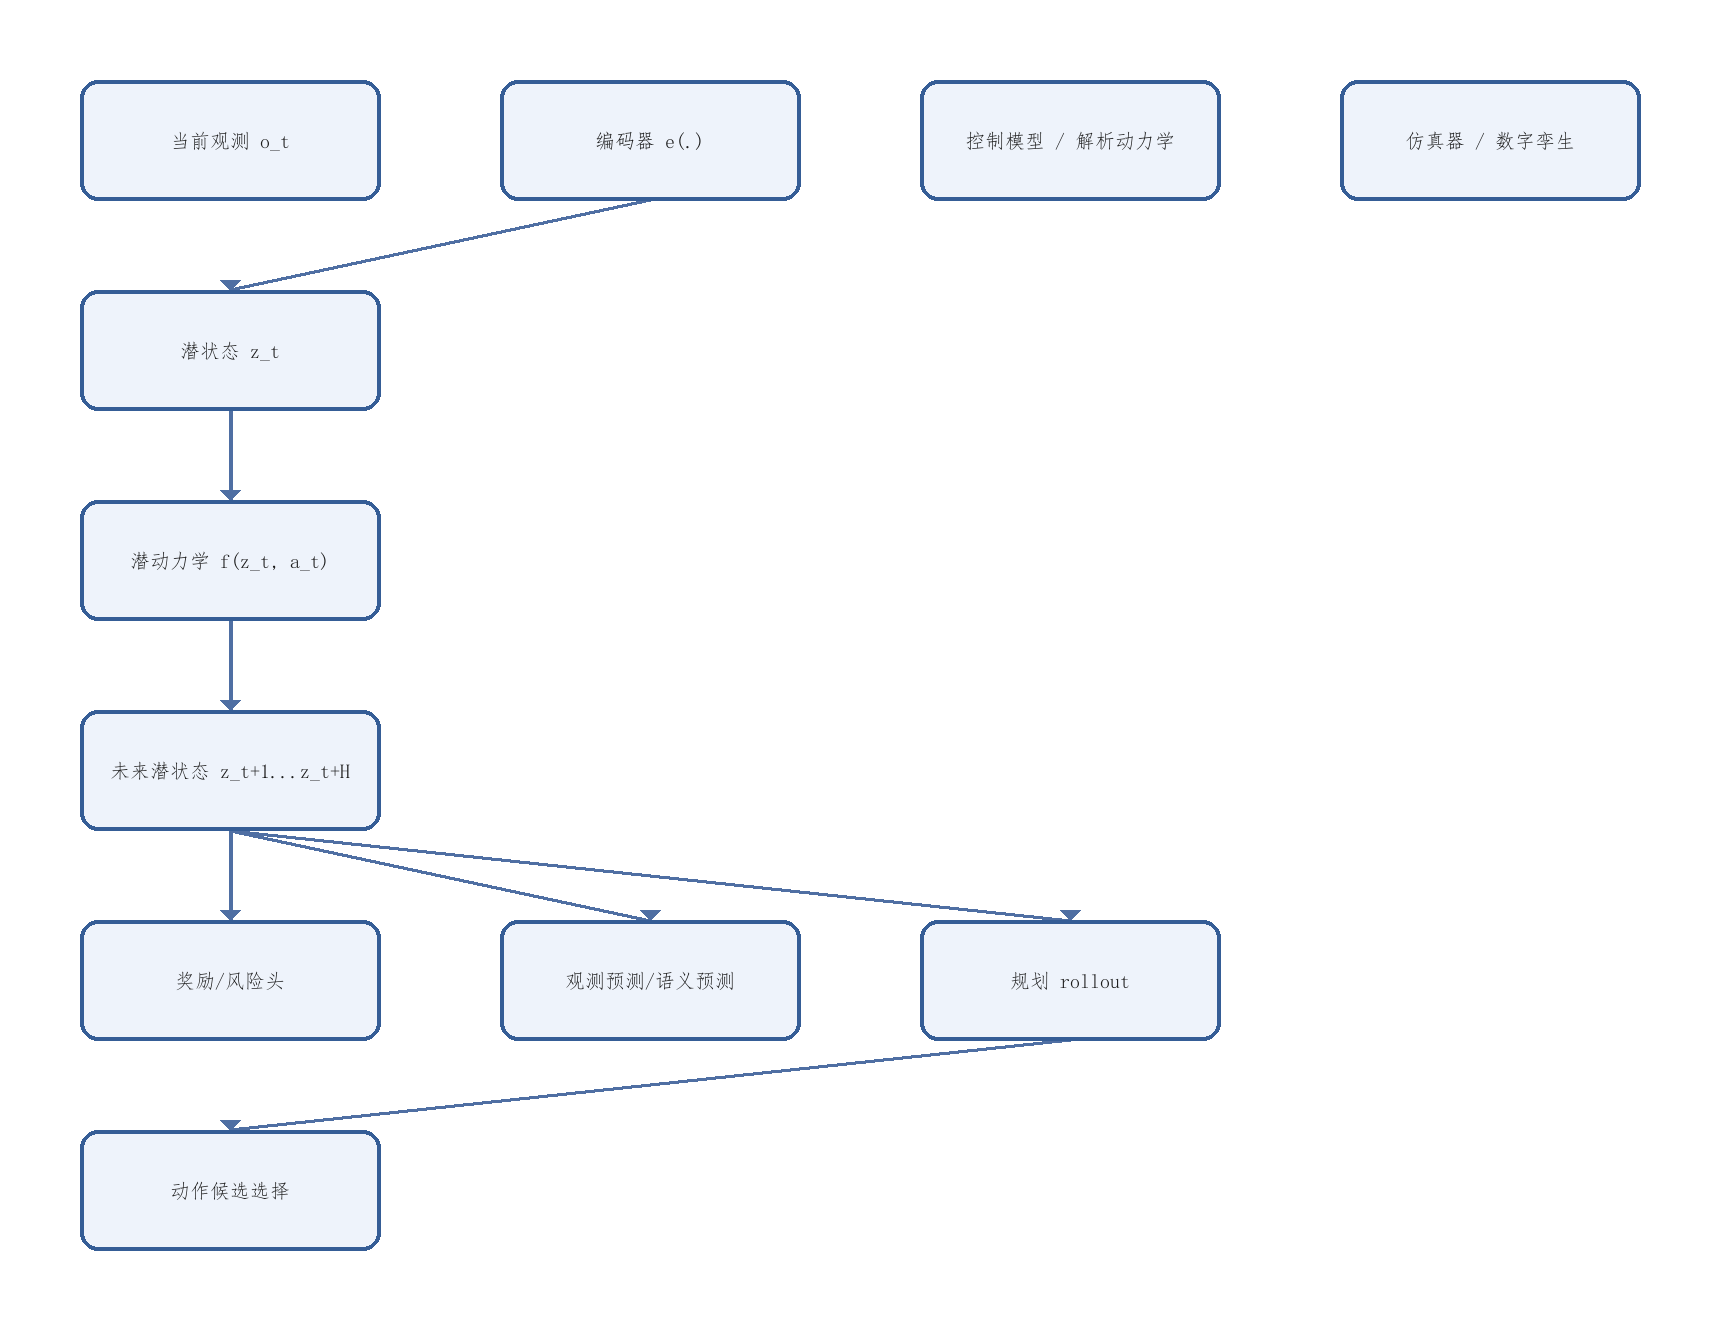
\includegraphics[width=0.9\textwidth,height=0.72\textheight,keepaspectratio]{figures/10-世界模型关系图.png}
\caption{10-世界模型关系图}
\label{fig:10-世界模型关系图}
\end{figure}

\input{chapters/11-VLA 与机器人基础模型}
% Generated from 12-规划、推理与决策的新路线.md; edit the LaTeX source after migration.

\reportpart{第十二部分 规划、推理与决策的新路线}
\addcontentsline{toc}{part}{第十二部分 规划、推理与决策的新路线}
\markboth{第十二部分 规划、推理与决策的新路线}{第十二部分 规划、推理与决策的新路线}

如果说第十一部分讨论的是如何把视觉、语言与动作统一成基础模型接口，那么本部分要回答的就是：这些模型如何真正承担任务结构化、长期决策和复杂场景下的推理责任。因为机器人并不只需要“输出动作”，还需要决定先做什么、后做什么、何时放弃、何时请求帮助、何时切换技能。于是，语言规划器、任务树、行为树、程序化中间表示、检索增强和多智能体协同等路线开始重新升温。

值得注意的是，规划问题在具身智能里从未消失，只是接口发生了变化。经典规划关注状态空间、动作集合与约束；基础模型时代则把自然语言、常识知识与长程结构化推理重新接入规划器。因此，这一章不应被理解为“旧规划 vs 新模型”的对立，而应被理解为“规划载体和规划接口的迁移”。 这种迁移在语言指导技能调用、代码生成式策略以及开放世界自主代理等路线中都有体现；相关代表性系统可参见 \href{https://arxiv.org/abs/2204.01691}{SayCan：语言指导技能调用}、\href{https://arxiv.org/abs/2209.07753}{Code as Policies：代码生成策略} 与 \href{https://arxiv.org/abs/2305.16291}{Voyager：开放世界自主代理}。

\section*{57. 语言规划与任务分解}
\addcontentsline{toc}{chapter}{57. 语言规划与任务分解}
\markboth{57. 语言规划与任务分解}{57. 语言规划与任务分解}

\subsection*{57.1 高层语言规划器}
\addcontentsline{toc}{section}{57.1 高层语言规划器}


高层语言规划器的最小职责，是把自然语言目标翻译成“可被下游技能层消费的任务结构”，而不是直接输出电机级动作。它通常接收三类输入：用户目标 \(g\)、当前环境观测 \(o_t\)、以及外部记忆或技能库描述 \(m\)。输出则往往是一组阶段化子任务、技能调用建议或带前置条件的候选计划。

若写成抽象形式，高层规划器更像是在估计：

\begin{equation*}
p(\tau \mid g, o_t, m)
\end{equation*}

其中 \(\tau = (u_1, u_2, \dots, u_K)\) 表示高层子任务序列。这个公式强调，高层规划本质上不是凭空“想步骤”，而是在目标、场景状态和可用技能约束下生成结构化任务图。为了让这个图能够真正流入执行层，一个更接近工程现实的计划节点往往至少要写成：

\begingroup
\scriptsize
\begin{equation*}
u_i = (\text{skill}, \text{object\_ref}, \text{goal\_region}, \text{constraint}, \text{success}, \text{fallback})
\end{equation*}
\endgroup

这里 \texttt{\detokenize{skill}} 指向可调用技能，\(object_ref\) 负责把语言指代绑定到对象状态，\(goal_region\) 给出目标区域或目标框架，\texttt{\detokenize{constraint}} 表示姿态容差、禁行区或资源限制，\texttt{\detokenize{success}} 定义成功条件，\texttt{\detokenize{fallback}} 则规定失败后回退、重观察或请求帮助的策略。把高层计划写成这种“半结构化契约”的意义，在于它把大模型最容易含糊带过的隐含前提全部显式化。

一个最小工作流通常可以写成：

\begin{lstlisting}[language=python]
goal = parse_user_goal(text_instruction)
scene = summarize_world_state(observation, memory)
skills = retrieve_available_skills(skill_registry, scene)
plan = llm_planner(goal=goal, state=scene, skills=skills)
\end{lstlisting}

但高层语言规划器真正困难的地方，不在于生成一串看起来合理的步骤，而在于这些步骤是否与系统真实能力边界一致。很多大模型在文本层面能够给出漂亮计划，却默认了隐含技能存在、对象状态可观测、执行顺序可行、失败可以无代价回滚等前提。机器人规划器若不能把这些隐含前提显式化，就会在真实执行时不断把“语义上合理”转化为“工程上不可执行”。

因此，高层规划器的主要职责不应被理解为“替所有层做决定”，而应被理解为“生成一组可被下游验证与编译的候选任务结构”。它越靠近这一职责，越容易与后续行为树、HTN、程序化中间语言和技能调度器形成稳定接口；它若直接越过这些接口输出含糊文本，就越容易在真实现场变成无法审计的黑盒建议器。

高层语言规划器的核心作用，是把自然语言目标转化为结构化子任务序列。例如，“整理桌面”可能被分解为识别对象、分类、抓取、放置和异常处理。大模型在这里的优势，在于它们天然擅长处理长文本目标、常识知识和任务组合关系。

\subsection*{57.2 子任务序列生成}
\addcontentsline{toc}{section}{57.2 子任务序列生成}


对子任务序列生成而言，最重要的不是“分解得多细”，而是分解出的每个节点是否具有明确输入、输出、前置条件和失败后的修复路径。一个好的子任务节点，往往至少要回答四个问题：做什么、依赖什么、成功如何判定、失败后如何回退或改写。

若把一个子任务节点记为 \(u_i\)，则更有操作性的表示不是一句自然语言，而是：

\begingroup
\footnotesize
\begin{equation*}
u_i = (\text{name}, \text{precondition}, \text{resource}, \text{success}, \text{fallback})
\end{equation*}
\endgroup

这种写法的重要性在于，它把“计划”从叙述文本改写成了可执行结构。很多高层规划失败，并不是因为模型不会分解，而是因为它输出的节点缺乏可消费字段，导致执行层既不知道何时开始，也不知道何时宣布成功，更不知道失败后应该退到哪一步。

若把这个节点继续展开成更接近执行器的接口，很多系统还会再补两类字段：

\begingroup
\scriptsize
\begin{equation*}
u_i^{exec} =
(\text{name}, \text{precondition}, \text{resource}, \text{timeout}, \text{verify}, \text{fallback})
\end{equation*}
\endgroup

这里 \texttt{\detokenize{timeout}} 用来避免技能长时间卡住而无人上抛，\texttt{\detokenize{verify}} 用来规定究竟由视觉、触觉、本体状态还是人类确认来宣布该节点完成。这个补充看似琐碎，实际上极为关键，因为很多“规划失败”并不是路径分解错了，而是节点完成判据和超时机制没有被写进任务结构。

因此，实际系统中的子任务生成常不是一次性文本生成，而是“生成 - 检查 - 修复 - 重排”的循环。其最小工作流可以写成：

\begin{lstlisting}[language=python]
plan = planner.generate(goal, state)
for subtask in plan:
    if not precondition_checker(subtask, world_state):
        subtask = planner.repair(subtask, world_state)
    if not skill_registry.supports(subtask):
        plan = planner.rewrite(plan, missing_skill=subtask)
\end{lstlisting}

因此，子任务序列生成应被理解为一个受约束的搜索问题，而不是单纯自然语言续写。一个好序列不仅要覆盖目标完成路径，还要包含前置条件、资源占用、互斥关系、超时处理和失败后可修复性。也正因如此，很多系统会在大模型生成后叠加技能可用性检查、状态谓词校验、行为树编译或候选计划重排序，而不是直接把文本计划下发给执行器。

更进一步说，子任务序列生成的真正难点是“计划图的结构正确性”而不是“句子是否通顺”。如果系统忽略资源冲突，同一时刻可能把机械臂和底盘同时调度到互相冲突的位置；如果忽略验证条件，技能层可能把“夹爪闭合”误判为“抓取成功”；如果忽略 fallback，整个系统会在一次局部失败后停成死局。也因此，规划器的质量在机器人里更应通过“能否稳定进入执行闭环”来判断，而不是通过语言流畅度来判断。

但生成子任务序列并不自动意味着这些子任务可执行。真正关键的问题是：这些子任务是否与现有技能库匹配，是否保留必要的前置条件，是否考虑执行中断和失败恢复。也就是说，语言规划器若没有与技能层和状态估计层对接，就仍然更像一个任务建议器。

\subsection*{57.3 指令歧义消解}
\addcontentsline{toc}{section}{57.3 指令歧义消解}


歧义消解真正困难的地方，不在于模型是否“理解中文”，而在于系统必须把语言中的模糊指代、隐含约束和环境依赖条件转写为后续可验证的任务对象。很多真实指令并不缺少语义，而是缺少执行边界，例如“顺手整理一下”“先处理危险的”“把它放回去”。如果没有把这些语句绑定到场景状态、对象候选集和任务阶段约束上，系统看似在理解语言，实际上是在冒险猜测。

机器人中的规划器必须频繁处理不完整指令。所谓“把那个杯子放回去”在纯文本中看似简单，到了真实场景却涉及对象指代、目标位置、省略步骤和历史上下文。规划器的价值因此不仅在于能输出计划，也在于能识别自己理解中的不确定性，并主动发起澄清。

若以 \(g\) 表示用户目标、\(m\) 表示外部记忆、\(o_t\) 表示当前观测，则高层规划器可抽象为：

\begin{equation*}
p(\tau \mid g, o_t, m)
\end{equation*}

其中 \(\tau = (u_1, u_2, \dots, u_K)\) 表示高层子任务序列。这个形式强调了现代规划器与经典 symbolic planner 的一个差异：它不再只依赖人工定义的状态谓词，也把语言上下文和记忆结构纳入了输入。

但真正的难点在于，歧义消解并不是单独的语言问题，而是“语言 - 场景 - 历史 - 技能库”四者的联合约束问题。同一句“把它放回原位”，在不同工作流、不同用户习惯和不同场景记忆下，可能对应完全不同的可执行计划。因此，一个成熟规划器不是更会猜，而是更会在不确定性过高时请求额外信息、调用外部记忆或回退到更保守的子任务。

若把歧义消解写成一个正式的决策门槛，它更接近：

\begingroup
\footnotesize
\begin{equation*}
\text{ask\_clarification} \Longleftrightarrow
H(\text{referent}\mid g,o_t,m) > \tau_H
\end{equation*}
\endgroup

这里 \(H(\cdot)\) 可以理解为对目标指代、目标位置或任务约束的不确定性。当不确定性高于阈值 \(\tau_H\) 时，系统最优行为不应是继续猜，而应主动澄清、重观察或降级执行。这个表达把“会提问”从体验优化重新压回安全与可执行性的必要条件：对具身系统而言，恰当地不执行，很多时候比勉强执行更智能。

\section*{58. 结构化决策中间表示}
\addcontentsline{toc}{chapter}{58. 结构化决策中间表示}
\markboth{58. 结构化决策中间表示}{58. 结构化决策中间表示}

\subsection*{58.1 行为树}
\addcontentsline{toc}{section}{58.1 行为树}


行为树之所以在机器人里长期流行，是因为它提供了一种介于脚本和规划器之间的结构化执行语义。它最常见的节点类型包括顺序节点、选择节点、条件节点和动作节点。系统在每个 tick 周期内从根节点向下传播执行请求，不同节点根据子节点返回的 \path{Success / Failure / Running} 状态决定是否继续、切换或回退。

一个最小行为树可以抽象为：

\begin{lstlisting}
Sequence
|- Condition: object_detected
|- Action: approach_object
|- Action: grasp_object
|- Fallback
   |- Action: place_in_bin
   |- Action: request_human_help
\end{lstlisting}

行为树在机器人和游戏 AI 中长期流行，并不是因为它最前沿，而是因为它在表达可回退、可条件切换、可并行调度的行为结构上非常实用。对具身系统而言，行为树仍然是把高层任务结构显式化的重要工具，相关综述可参见 \href{https://arxiv.org/abs/1709.00084}{《Behavior Trees in Robotics and AI》}。 如果把行为树放回具身系统的工程现实中，它的最大优点不是“优雅”，而是把失败传播规则写得非常明确。顺序节点意味着某一步失败会阻断整条链路，选择节点意味着系统在候选动作之间做退路切换，\texttt{\detokenize{Running}} 状态则给执行层留下持续闭环的时间窗口。对于真实机器人，这种显式失败语义非常关键，因为很多高层计划并不是一次性成功，而是在“执行中等待”“局部失败切换备选”“条件满足后继续”之间循环前进。 行为树的局限也应当讲清楚。它擅长表达局部决策流和异常回退，但不擅长自动发明新结构，也不擅长在开放场景中自己扩展词汇表。也正因如此，它在当前架构里更适合扮演“规划结果的执行编译层”而不是“唯一智能体”。大模型或高层规划器负责提出候选结构，行为树负责把这些结构转成具备明确 tick 语义、失败传播规则和恢复分支的执行图，这才是两者更稳健的分工。

\subsection*{58.2 任务树与 HTN}
\addcontentsline{toc}{section}{58.2 任务树与 HTN}


HTN（Hierarchical Task Network）可以理解为“把一个抽象任务通过一组分解规则逐步改写成可执行任务网络”。与行为树更强调运行时控制流不同，HTN 更强调规划时的任务展开过程。它通常包含抽象任务、原子任务以及分解方法。

一个极简 HTN 风格分解示意可以写成：

\begin{lstlisting}
Task: clean_table
-> Method A:
   detect_objects
   sort_by_category
   move_category_items
   verify_surface
\end{lstlisting}

HTN 之所以在今天依然有价值，恰恰因为它能把“语言生成出来的模糊层级结构”压缩成带有明确父子依赖、分解规则和可验证前置条件的图结构。对于具身系统，这意味着高层规划不必一次性承担全部细节，而可以把任务分解过程稳定绑定到一组可复用模板上。这样做虽然牺牲了一部分开放性，却往往换来了更强的可调试性、可回退性和跨团队协作可维护性。

层级任务网络（HTN）及类似结构的价值，在于它们能把复杂任务表示为多层目标分解图。这类方法非常适合和语言规划器结合：大模型负责提出候选高层结构，HTN 或任务树负责把它约束成更可执行的形式。

若把 HTN 写成更接近算法接口的形式，可以表示为：

\begingroup
\footnotesize
\begin{equation*}
T^{(k+1)} = \operatorname{Refine}(T^{(k)},\ \mathcal{R},\ s_t)
\end{equation*}
\endgroup

其中 \(T^{(k)}\) 是第 \(k\) 层任务图，\(\mathcal{R}\) 是分解规则集合，\(s_t\) 是当前状态。这个递推式的意义在于强调：HTN 的核心不是一次性给出完美分解，而是在状态约束和规则库作用下逐层收缩任务图，直到剩下能够被技能层直接消费的原子节点。对于具身系统，这种逐层收缩比自由文本分解更容易维护前置条件、资源互斥与失败恢复逻辑。

更进一步说，HTN 在今天重新变得重要，并不是因为它“比大模型更聪明”，而是因为它恰好提供了大模型最缺的一层结构化收束。语言模型可以快速提出若干分解候选，但这些候选常常缺少可验证前置条件、资源约束与回退逻辑；HTN 则恰好把这些信息放回任务表示本身。因此，两者更合理的关系不是替代，而是“生成候选层级结构”与“把候选压成可执行图结构”的分工。

若把这一过程写成更接近系统实现的形式，它往往会包含一个候选检索与可行性过滤过程：

\begingroup
\scriptsize
\begin{equation*}
\mathcal{M}^{*}(\tau, s_t)=
\left\{
m\in\mathcal{M}(\tau)\ \middle|\ 
\operatorname{Pre}(m)\subseteq s_t,\ 
\operatorname{Res}(m)\subseteq R_t
\right\}
\end{equation*}
\endgroup

这里 \(\mathcal{M}(\tau)\) 表示任务 \(\tau\) 的候选分解方法集合，\(\operatorname{Pre}(m)\) 表示前置条件，\(\operatorname{Res}(m)\) 表示资源需求，\(R_t\) 表示当前资源状态。这个过滤步骤的作用，是把“看起来像合理计划”的文本候选，压缩成“在当前状态下真的可以展开”的方法集合。

从工程角度看，HTN 的典型失败模式也很明确。第一类是方法库陈旧，导致高层还能分解，落到技能层却已经找不到合法执行器；第二类是世界状态估计错误，前置条件判断失真，使系统在不具备条件时仍错误展开任务；第三类是异常恢复未被写入分解规则，导致计划一旦偏离主路径就只能整棵树推倒重来。因此，HTN 的长期价值不只在于静态分解，而在于它是否把“检索、验证、重规划与回退”一起写进任务组织协议。

\subsection*{58.3 程序化中间语言}
\addcontentsline{toc}{section}{58.3 程序化中间语言}


程序化中间语言的核心思想，是让大模型输出的不是“自由文本计划”，而是一个带类型约束、参数槽位和可调用 API 的半结构化程序。它既保留语言模型对开放语义的表达能力，又通过语法和工具接口把行为限制在可解释、可验证的执行边界内。

一个最小示意可以写成：

\begin{lstlisting}[language=python]
plan = [
    Pick(object="red_cup", grasp="top"),
    MoveTo(location="right_tray"),
    Place(object="red_cup", tolerance="fragile")
]
\end{lstlisting}

与自由文本相比，这种中间语言至少带来三点价值：第一，参数槽位可以被感知模块重新绑定；第二，动作类型可以被白名单与安全规则约束；第三，执行日志更容易被回放和审计。它的代价则在于表达空间被收紧，因此必须设计得既足够结构化，又不能过早把开放任务压扁。

一个极简 DSL 片段可以写成：

\begin{lstlisting}[language=python]
if detect("mug", table="left"):
    grasp("mug")
    place("mug", target="sink")
else:
    ask_human("Where is the mug?")
\end{lstlisting}

程序化中间语言的出现，反映的是一种很现实的架构需求：直接从文本到动作太脆弱，而纯符号系统又太僵硬，因此需要一种既保留语义结构、又便于执行验证的中间形式。机器人编排 DSL、技能脚本和可调用接口风格接口都可视为这一路线的不同变体。Code as Policies 的代表性恰恰在于，它把语言模型输出约束到可执行代码接口，使“推理”更容易经过解释器、类型约束和工具调用链路，相关论文可参见 \href{https://arxiv.org/abs/2209.07753}{Code as Policies 论文}。

\subsection*{58.4 神经符号混合方案}
\addcontentsline{toc}{section}{58.4 神经符号混合方案}


神经符号混合方案之所以反复出现，是因为它试图把两类互补能力放在一起：神经模型擅长从复杂感知输入中提取柔性的表征与启发式，符号规划擅长维护显式约束、长时程结构和可验证的状态转移。对机器人而言，这种混合路线的核心吸引力，不是理论优雅，而是它更容易在开放感知与受约束执行之间建立桥梁。

但这条路线也并不轻松。最大难点通常不是“如何把神经网络接上规划器”，而是状态抽象是否足够稳定，能否让高层符号变量真正对应到现场可观测、可执行、可恢复的对象与关系。若抽象层不稳，神经符号混合就会退化成接口复杂但并不可靠的双系统叠加。 从系统实现角度看，神经符号混合通常可以被写成三层闭环：先用神经感知模块把视觉、语言和状态历史压缩成任务相关表征；再由符号层执行约束检查、技能选择和顺序编排；最后由执行层把失败信号、状态偏差和资源冲突反向返回给上层。真正有用的不是“符号味更重”或“神经味更重”，而是这三层之间是否形成了可追责的接口。如果研究工作只展示了神经模块很强、或符号结构很漂亮，但没有解释失败如何回传、约束如何触发、技能如何重写，那么它对部署的帮助仍然有限。

神经符号混合方案持续有吸引力，是因为它试图同时保留两类优势：神经方法对感知噪声、模糊模式和高维输入的适应能力，以及符号方法对约束表达、组合泛化和可解释推理的优势。对具身系统而言，这种混合并不是理论上的折中，而往往是现实系统里最自然的分工方式。

但这类方案真正困难的地方并不在于“把两个模块接起来”，而在于定义两者之间稳定且不过度脆弱的接口。若感知输出无法支撑符号层需要的确定性，或者符号层给出的计划无法被低层连续动作执行，混合方案就会在接口处失效。 从工程现实看，神经符号混合方案的吸引力还在于责任切分更清楚。神经模型负责处理开放词义、长尾语境和模糊常识，符号或程序结构负责处理类型约束、顺序约束、权限边界和失败分支。这种分工并不总能获得最惊艳的 demo，但更容易形成可测试接口和问题归因路径，因此尤其适合那些需要长期维护、要通过审计或要进入高风险场景的机器人系统。

神经符号路线的真正意义，不在于“把老符号 AI 重新包装”，而在于它提供了一种可能：让语义理解依赖神经模型，让可验证结构依赖显式程序或逻辑结构。对需要长期可靠部署的机器人系统而言，这种混合路线往往比纯端到端推理更有工程吸引力。

更进一步说，神经符号混合最值得重视的不是理论姿态，而是它往往天然提供了更清楚的责任切分。神经部分负责吸收开放语义、长尾环境和感知噪声，符号或程序部分负责约束顺序、权限、前置条件和异常分支。对于需要长期维护、要通过审计或要进入高责任场景的系统，这种可切分性本身就是工程价值。

\section*{59. 大小脑协同范式}
\addcontentsline{toc}{chapter}{59. 大小脑协同范式}
\markboth{59. 大小脑协同范式}{59. 大小脑协同范式}

\subsection*{59.1 语义级决策与运动级执行的接口}
\addcontentsline{toc}{section}{59.1 语义级决策与运动级执行的接口}


这个接口最值得重视的地方，是它决定了高层错误会以何种方式传递到低层。若接口过粗，低层会被迫在信息不足的前提下猜测目标细节；若接口过细，高层又会把自己并不擅长的连续控制细节硬塞给执行器。成熟系统通常会在这一层显式写出中间契约：目标对象是谁、目标区域在哪里、允许的接近方式有哪些、失败后应该在本层修复还是上抛重规划。没有这层契约，语义规划和运动执行就很难形成稳定协作。 这一接口的本质，是把“高层说什么”和“低层怎么把它做出来”分开描述。语义级决策通常输出的是技能名、子目标、目标对象或目标区域；运动级执行则需要这些抽象变量被具体绑定成轨迹、末端位姿、接触约束和控制频率。因此，一个真正可用的接口必须至少完成四件事：目标绑定、状态对齐、可达性检查、执行中反馈回传。

可以把这个接口抽象为：

\begin{equation*}
u_t = \mathrm{Bind}(g_t, \hat{x}_t, \mathcal{K})
\end{equation*}

其中 \(g_t\) 是高层语义目标，\(\hat{x}_t\) 是当前估计状态，\(\mathcal{K}\) 是技能库或控制器集合，\(u_t\) 则是可交给执行层的具体技能或控制命令。若把这一绑定结果继续写成一个可审计契约，通常更接近：

\begingroup
\scriptsize
\begin{equation*}
g_t^{exec} =
(\text{skill}, \text{target\_frame}, \text{tolerance}, \text{guard}, \text{stop}, \text{fallback})
\end{equation*}
\endgroup

这里 \(target_frame\) 表示目标位姿或目标区域绑定在哪个坐标系，\texttt{\detokenize{tolerance}} 规定允许的误差边界，\texttt{\detokenize{guard}} 表示碰撞、力觉或禁区等守卫条件，\texttt{\detokenize{stop}} 表示执行完成或应立即停机的判据，\texttt{\detokenize{fallback}} 则说明失败是局部重试、重观察，还是直接上抛高层重规划。这个结构的关键意义在于，它把“语义目标”翻译成了“控制层知道如何执行、何时停止、何时拒绝执行”的工程对象。

也正因此，很多表面上看似简单的接口失效，本质上都不是模型不会生成动作，而是契约字段不完整。高层若只说“把杯子拿到托盘”，低层仍然要补全是抓杯身还是抓杯沿、托盘坐标系是谁定义的、接近是否允许扫过禁区、滑移后是否应立刻回退。这些问题越是没有被正式写入接口，系统越依赖隐含假设和人工兜底。

大小脑分层的核心不是一个比喻，而是架构现实：高层决策频率低、语义密度高；低层执行频率高、连续性强。二者若不分层，系统难以同时满足长期任务理解和短时稳定控制的要求。

\subsection*{59.2 调度频率与时间尺度问题}
\addcontentsline{toc}{section}{59.2 调度频率与时间尺度问题}


这也是为什么“统一模型每一步都重新思考一切”的设想在真实系统里往往并不划算。高层推理一旦太频繁，就会把计算预算浪费在重复解释任务上；太稀疏，则会让计划对局部异常反应迟缓。调度频率设计本质上是在决定：哪些问题值得重新思考，哪些问题应交给局部控制器自动吸收。这个问题没有通用最优解，只能结合任务节奏、硬件时延、传感刷新频率和安全约束做系统级折中。

更具体地说，规划系统通常至少有三种时钟：感知刷新时钟、局部控制时钟和高层重规划时钟。三者若没有被清楚区分，系统就会出现一种常见错觉，即“模型总在忙，但系统并不更稳”。真正成熟的调度设计，往往不是让所有模块同步全速运转，而是让每一层只在自己真正需要更新的时候工作。

很多看似“模型能力不够”的问题，本质上其实是时间尺度错配：高层推理太慢，低层反馈太快；高层生成的计划太粗，低层执行需要更细；高层上下文太长，低层状态新鲜度要求更高。因此，调度频率本身就是系统设计变量。

若高层每 \(\Delta T_H\) 秒更新一次计划，低层每 \(\Delta T_L\) 秒闭环一次控制，通常需要满足：

\begin{equation*}
\Delta T_H \gg \Delta T_L
\end{equation*}

并且高层计划误差不能在 \(\Delta T_H\) 时间窗口内失控地积累。这也是为什么许多系统宁愿牺牲一点“统一性”，也要保留局部反射与中层技能缓存。

更工程化地说，系统往往不是简单满足 \(\Delta T_H \gg \Delta T_L\) 就足够，还要满足高层计划在一个更新窗口内不过期。若以 \(v_{\text{env}}\) 表示环境变化速度、\(\epsilon_{\text{plan}}\) 表示高层计划可容忍误差，则一个更实用的条件是：

\begingroup
\footnotesize
\begin{equation*}
v_{\text{env}} \cdot \Delta T_H \le \epsilon_{\text{plan}}
\end{equation*}
\endgroup

这个不等式提醒我们，高层更新时间并不是抽象调参问题，而由环境变化速度直接约束。相同的 planner 放到静态分拣工位和动态人机协作场景中，最优更新频率可能完全不同。因此，调度频率应被看成部署变量，而不是论文实现细节。

这还意味着调度问题不能只靠固定频率解决，往往还需要事件触发式重规划。很多系统在平稳阶段完全不必让高层持续重算，而一旦出现目标丢失、资源冲突、接触失败、语义歧义或外部人类插入动作，高层又必须立即介入。更贴近工程的设计，通常是“低频周期重规划 + 高频事件触发重规划”的混合机制，而不是单一时钟。

若令一个高层更新窗口中可容纳的低层闭环次数为 \(N_{\text{low}}\)，则有：

\begin{equation*}
N_{\text{low}}=\frac{\Delta T_H}{\Delta T_L}
\end{equation*}

这个量很适合帮助读者建立直觉。因为它直接告诉我们：当高层一次决策尚未刷新时，低层控制器已经独立闭环了多少次。只要 \(N_{\text{low}}\) 很大，高层计划就必然只能承担方向性职责，而不能假装自己仍在逐步控制细节。后文看到任何“统一决策器”路线时，都应把它放回这个比例关系里判断其职责边界。

因此，调度频率问题本质上是在决定责任分层。高层负责多久一次重新解释目标、何时修改计划骨架、何时请求澄清；中层负责在该骨架下多快地重新参数化技能；低层则负责在更快时间尺度内吸收扰动。只要这三层责任没有随着时间尺度一起被明确，所谓“统一智能体”在真实部署中往往会退化成一组互相等待、互相遮蔽错误来源的松散模块。

\subsection*{59.3 现实系统中的工程折中}
\addcontentsline{toc}{section}{59.3 现实系统中的工程折中}


现实系统中的工程折中，往往意味着规划与推理不会以最纯粹的论文形式出现。为了满足时延、稳定性和可维护性要求，企业系统常常会保留大量启发式规则、预定义技能、状态机和本地恢复逻辑，再在部分环节引入学习型规划或大模型推理。表面上看这不够“统一”，但往往更可交付。

因此，理解规划路线时不应只问“是否端到端”，而应问“哪些层必须保留折中，为什么”。很多看似不够优雅的工程设计，恰恰是在系统真实进入现场后才被证明必要的部分。 更进一步说，工程折中并不是“学术不纯粹”的副产品，而是具身系统从研究走向交付时必须显式回答的架构问题。一个规划器若只能在理想状态下输出全局优解，但无法在传感掉帧、技能不可用或人为插入任务时快速降级，那么它在真实系统里反而不如一个次优但可回退的方案有价值。也正因此，本章讨论的规划与推理路线，最终都应该被放回 15、16 两章中的部署与安全约束下再评价。

现实系统中的工程折中，常常体现在研究论文最不愿展开的地方：是选择更高性能但更不稳定的规划器，还是选择更保守但更可验证的方案；是让模型更自主，还是保留更多手工规则与安全裁剪；是追求端到端统一，还是接受分层带来的复杂性。真正上线的系统几乎都在这些地方做过妥协。

也正因此，判断一条路线是否成熟，不能只看它最强时能做到什么，更要看它在资源有限、时延受限、安全约束存在、维护压力真实存在时，最终选择了怎样的工程边界。很多看似“不够优雅”的折中，恰恰是现实可交付性的来源。 因此，现实系统里的“规划器”往往不是单个模块，而是一条多层责任链。高层决定意图与阶段，中层维护技能切换与条件恢复，底层保证轨迹与接触稳定，外层再由安全监督器监控越界行为。看起来不够优雅，但这正是大量真实机器人产品能够工作的原因。评价论文或企业方案时，若只看最上层模型而忽略这条责任链，很容易高估其统一程度、低估其工程支撑。

现实中的大小脑系统常常不是严格两层，而是多层：高层语义规划、中层技能调度、低层闭环控制再加安全监控。这种复杂性并不意味着设计失败，而恰恰说明真实机器人系统很难被单一时间尺度统一吞并。

\section*{60. 连续推理与外部记忆}
\addcontentsline{toc}{chapter}{60. 连续推理与外部记忆}
\markboth{60. 连续推理与外部记忆}{60. 连续推理与外部记忆}

\subsection*{60.1 推理 token 在机器人中的局限}
\addcontentsline{toc}{section}{60.1 推理 token 在机器人中的局限}


因此，机器人并不是“把更多思维链搬过来”就会自然变强。推理 token 的价值只在于它是否帮助系统减少了高代价错误、改善了阶段切换、增强了异常解释或提高了澄清提问质量。如果额外推理带来的只是更长的文本、更慢的响应和更过时的状态判断，那么它反而会恶化闭环质量。对具身系统而言，推理预算始终必须服从物理时钟，而不是反过来让物理世界等待语言模型思考。 把更多推理 token 投入机器人，并不自动等于更好的行为，因为机器人决策不是纯文本推理，而是受状态新鲜度约束的实时闭环。每多做一轮长链推理，环境都可能已经变化：人移动了、物体被遮挡了、夹爪姿态漂了、目标已经不在原处。因此，机器人中的“多想一步”始终要与“是否来得及执行”一起评价。

若用一个很简单的时延模型表达，可以把总决策延迟写成：

\begingroup
\footnotesize
\begin{equation*}
T_{\text{decision}} = T_{\text{perception}} + T_{\text{reason}} + T_{\text{actuation}}
\end{equation*}
\endgroup

推理 token 可以帮助高层任务思考，但机器人系统不能无代价地无限推理。原因并不神秘：推理消耗时间、时间会导致状态陈旧、状态陈旧会削弱动作可执行性。因此，机器人中的“更会想”必须始终和“还能够及时做”一起被评价。

若再把状态陈旧的代价显式写出来，则高层推理是否值得继续，往往取决于：

\begingroup
\footnotesize
\begin{equation*}
\Delta V_{\text{reason}} > C_{\text{staleness}}(T_{\text{reason}})
\end{equation*}
\endgroup

其中左边代表额外推理带来的决策价值增量，右边代表由于状态陈旧而带来的执行损失。这个比较的意义，在于把“推理 token 越多越好”的直觉改写成一个部署问题：只有当额外推理确实减少高代价失误、并且收益大于时延代价时，推理才应继续扩展。否则，系统更适合切回局部技能、缓存策略或保守回退。

更实用的系统设计，通常会把“是否继续推理”也做成一个门控决策，而不是默认无限展开思维链。例如：

\begingroup
\scriptsize
\begin{equation*}
\text{reason\_more}
\Longleftrightarrow
U_{\text{uncertainty}} + U_{\text{novelty}} + U_{\text{risk}} > \tau
\end{equation*}
\endgroup

其中 \(U_{\text{uncertainty}}\) 表示当前任务语义或状态解释的不确定性，\(U_{\text{novelty}}\) 表示是否遇到超出缓存技能分布的新情形，\(U_{\text{risk}}\) 则表示若直接执行可能导致的安全或代价损失。这个门槛并不要求精确估计，只要求系统显式承认：推理预算应当在“值得多想”的时候被调用，而不是在每一步都平均摊开。

因此，推理 token 在机器人里更适合承担三类职责。第一类是语义歧义消解，例如判断指令里的“那个杯子”究竟是哪一个；第二类是阶段切换解释，例如从抓取切到放置或从失败恢复切到重新观察；第三类是异常复盘，例如说明为什么当前技能应该被打断或替换。相反，若任务已经进入高频接触控制、动态平衡或连续轨迹跟踪阶段，那么继续增加语言推理往往收益很低，因为真正限制系统的是低层反馈带宽，而非高层语义推演。

\subsection*{60.2 外部记忆与检索增强}
\addcontentsline{toc}{section}{60.2 外部记忆与检索增强}


外部记忆可以理解为“把不适合塞进当前上下文窗口、但又会反复影响任务成败的状态与经验结构化存放起来”。它通常至少包含三类对象：环境记忆、任务记忆和人机交互记忆。

如果把记忆系统设计成研究对象而不是附属缓存，就会发现它至少要回答三个问题：写入什么、何时失效、如何检索。环境记忆更像地图与对象历史，任务记忆更像阶段日志与失败片段，人机交互记忆则更像约束、偏好与澄清记录。三者在时间有效性和可信度上都不同，因此不能简单混在一条文本上下文里。

若把外部记忆抽象成一个正式数据结构，则最小条目可以表示为：

\begingroup
\footnotesize
\begin{equation*}
M_i = (\text{key}, \text{type}, t_i, \rho_i, \mathrm{ttl}_i, p_i)
\end{equation*}
\endgroup

其中 \texttt{\detokenize{key}} 是索引键，\texttt{\detokenize{type}} 区分环境、任务或交互记忆，\(t_i\) 是写入时间，\(\rho_i\) 表示置信度或来源可靠性，\(\mathrm{ttl}_i\) 表示失效窗口，\(p_i\) 则是负载内容。把记忆显式写成这个结构的意义，在于提醒我们：机器人记忆并不是“多一段上下文文本”，而是一套必须被权限、时效性和来源可信度共同约束的数据基础设施。

一个最小检索增强工作流可以写成：

\begin{lstlisting}[language=python]
query = build_context_query(goal, observation)
memory_items = retrieve(memory_store, query)
augmented_state = fuse(observation, memory_items)
plan = planner(goal, augmented_state)
\end{lstlisting}

若把检索动作进一步形式化，可以写成：

\begingroup
\footnotesize
\begin{equation*}
\mathcal{M}_t = \operatorname{TopK}\!\left(q_t,\{M_i\}_{i=1}^{N}, k\right)
\end{equation*}
\endgroup

其中 \(q_t\) 由当前目标、观测、任务阶段和可用技能共同构成。这个式子说明，记忆系统最关键的不是“能存多少”，而是能否围绕当前任务阶段检索出少量真正有用、且尚未过时的条目。对机器人来说，外部记忆的价值尤其体现在“让系统不必每次都重新从零理解现场”。相同房间布局、重复出现的工具、用户偏好、历史失败点、危险区域和常用收纳位置，都更适合以显式可检索结构保存，而不是期待大模型在隐式参数里长期稳定记住。这样做不仅提升长期任务连续性，也使得记忆本身能够被审计、修订和按场景权限管理。

与其让模型在参数中隐式记住一切，不如将环境历史、任务历史、对象属性和用户偏好外置为检索结构。这对长期任务特别重要，因为机器人系统会持续遇到相似场景、相似对象和相似失败模式。

\subsection*{60.3 历史轨迹、场景状态与人类反馈的融合}
\addcontentsline{toc}{section}{60.3 历史轨迹、场景状态与人类反馈的融合}


真正困难的部分，则在于这些异构记忆如何被统一索引和可信消费。文本反馈、轨迹片段、对象状态快照和视频回放往往有不同时间粒度、不同置信度和不同用途，系统若简单拼接，很容易导致检索污染或过时记忆误导当前决策。因此，外部记忆不是“存得越多越好”，而是要围绕任务阶段、时间有效性、来源可信度和与当前技能接口的相关性来做结构化管理。

把这种融合写成一个更清楚的接口，可以表示为：

\begingroup
\footnotesize
\begin{equation*}
\tilde{s}_t = \mathrm{Fuse}(o_t, x_t, \mathcal{M}_t, h_t^{human})
\end{equation*}
\endgroup

其中 \(o_t\) 是当前外部观测，\(x_t\) 是机器人自身状态，\(\mathcal{M}_t\) 是检索到的历史轨迹与场景记忆，\(h_t^{human}\) 则代表来自人类的纠正、偏好或澄清。这个形式说明，历史轨迹、场景状态和人类反馈不是三条平行文本，而是共同构成“当前该怎么决策”的增强状态。真正实用的机器人记忆通常不是纯文本记忆，而是多模态任务记忆：轨迹片段、地图状态、对象位置、失败案例和人类纠正记录共同构成可检索上下文。SayCan 的技能可供性评分、Voyager 的代码技能库积累，以及长程代理系统中的记忆缓冲区，本质上都属于把“推理”嵌入外部结构而不是完全内化在一次前向传播里，相关工作可参见 \href{https://arxiv.org/abs/2204.01691}{SayCan} 与 \href{https://arxiv.org/abs/2305.16291}{Voyager}。

如果进一步从消费者角度看，记忆必须按时间尺度分层暴露。第一层是毫秒到数十毫秒级的稳定控制层，负责阻抗、跟踪、接触稳定和安全停机；第二层是数百毫秒到数秒级的技能层，负责抓取、开门、对位、避障等可复用技能；第三层才是秒级到分钟级的语义规划层，负责“先做什么、后做什么、是否换策略”。不同层消费记忆的方式并不相同：控制层更关心局部接触与即时状态，技能层更关心最近几步成败与对象位置，规划层更关心任务历史、用户偏好和长期约束。如果把本应在前两层解决的问题一股脑上推给高层大模型，就会出现“推理上很聪明、动作上总是慢半拍”的典型失配。

这也意味着，“大脑-小脑-脊髓”并不是修辞，而是不同更新频率、不同可验证性和不同失败代价的真实分层。一个可部署系统通常需要显式规定每层预算，例如：

\begin{lstlisting}
high-level planner:   0.5-2 Hz
skill scheduler:      2-10 Hz
feedback controller:  100-1000 Hz
safety monitor:       event-triggered
\end{lstlisting}

如果这套频率预算没有在系统设计早期被固定下来，后续很多争论都会变得含混不清。研究者会误以为自己在比较模型优劣，实际上比较的常常是不同时间尺度上的职责分配。

从系统风险角度看，外部记忆至少有三种常见失效模式。第一种是过时记忆污染当前决策，例如对象已经被人移动，系统却仍按照历史位置规划；第二种是错误抽象，把一次偶然成功的局部策略写成通用规则；第三种是权限越界，例如把用户偏好日志和场景危险区域记录混在同一检索空间中。真正成熟的记忆增强系统，通常会把“能否写入”“谁能读取”“什么条件下失效”设计得和模型本体同样严肃，而不把记忆当作随手加上的缓存层。\href{https://arxiv.org/abs/2204.01691}{SayCan} 与 \href{https://arxiv.org/abs/2305.16291}{Voyager} 分别从技能可供性和技能积累角度，展示了外部结构对长期决策的重要性。

\section*{61. 多机器人与多智能体协同}
\addcontentsline{toc}{chapter}{61. 多机器人与多智能体协同}
\markboth{61. 多机器人与多智能体协同}{61. 多机器人与多智能体协同}

\subsection*{61.1 分工与通信}
\addcontentsline{toc}{section}{61.1 分工与通信}


多体协作中的分工与通信，不能只理解成多台机器人互相发消息。更核心的问题是：谁负责全局任务拆分，谁负责局部执行，哪些状态必须共享，哪些状态只需要本地维护，以及一旦通信延迟或局部失败出现，系统如何退化运行。没有这些设计，协作系统很容易在规模扩大后迅速失稳。

因此，多机器人协作的难点不只是算法复杂度增加，而是组织复杂度上升。它要求我们把原本单机内部的规划、调度、资源分配和异常恢复问题，提升到跨主体层面重新设计。 这里很适合引入一个最小通信契约的视角。对于多机器人或多模块系统而言，真正必须共享的往往不是全部观测，而是少量高价值变量，例如任务占用、空间占用、资源锁、异常状态和阶段完成信号。凡是能通过局部闭环解决的问题，最好不要升级成全局通信问题；凡是会引发级联冲突的问题，则必须被提升为全局可见状态。这个原则比单纯强调“大模型负责协调一切”更贴近真实工程。

多智能体或多模块系统中的“分工与通信”并不是一个附属问题，而是决定系统复杂性是否真正可控的核心问题。只要任务被拆到多个执行体、技能模块或推理层次之间，就必须回答谁负责全局目标、谁处理局部异常、哪些状态需要共享、哪些决策可以局部独立完成。

通信设计过少，会让各模块各自最优却整体失调；通信设计过多，则会迅速抬高系统延迟、协调成本和调试难度。对具身系统来说，更现实的方向通常不是追求完全自由通信，而是围绕任务结构设计稀疏、稳定、语义明确的交互协议，让系统在必要时共享关键状态，而不是在所有时刻交换所有信息。

若把多体协作中的最小通信对象压缩一下，一个更贴近系统实现的形式是：

\begingroup
\scriptsize
\begin{equation*}
\mu_{i\rightarrow j} = (\text{task id},\ \text{resource claim},\ \text{status},\ \text{deadline},\ \text{handover condition})
\end{equation*}
\endgroup

这里最关键的信息并不是原始观测，而是任务占用、资源锁、超时边界和接管条件。因为真实协作系统失败的常见原因，往往不是“看不见彼此”，而是“不知道谁已经占用了同一工位、谁应该等待、谁应该接管”。因此，多机器人通信设计首先是组织协议设计，而不是带宽竞赛。

多机器人协同把单体系统的问题放大成协调问题：谁先做、谁等待、谁搬运、谁观察、谁承担共享地图维护。语言模型与多智能体规划看起来在这里很有吸引力，但真正难的是通信延迟、信息不一致和角色切换的可验证性。

因此，多智能体规划的核心并不是“让多个智能体都更聪明”，而是让它们在信息不完全同步的情况下仍维持足够稳定的组织秩序。现实部署中，协作失败往往不是因为单体不会做事，而是因为局部错误状态被广播、放大并演化成系统性失调。

\subsection*{61.2 协作任务的规划难点}
\addcontentsline{toc}{section}{61.2 协作任务的规划难点}


从算法视角看，这意味着协作规划往往隐含一个带约束的联合优化问题：每个体的局部最优行动，必须接受全局资源和时序一致性的裁剪。很多看起来“单机上已经成熟”的技能，一旦进入多机协同，就必须增加资源仲裁、超时重分配和状态对账机制。读这一节时，最好把“多机协同”理解为把单体闭环复制多份之后，再额外叠加一层组织系统，而不是把单体技能简单并联。

协作任务的规划难点，在于系统不再只需预测环境和自身，还需要预测其他主体的时序、意图、误差与反应方式。无论对方是人类操作者、另一台机器人还是上位调度系统，只要它们的行为不完全可控，规划问题就会从单体优化迅速变成带有不完全信息和动态博弈色彩的协调问题。

这意味着协作规划往往比单体任务更依赖显式协议、角色分工、冲突消解与可解释状态交换。若这些机制缺失，即使单个执行体能力很强，整体系统也可能因为协调代价过高而失去效率与稳定性。 更麻烦的是，协作系统中的失败往往不是独立失败，而是耦合失败。一个机器人迟到一步、误占一个工位、误判一件对象状态，都可能让其他机器人基于错误前提继续执行，从而把局部偏差快速放大成系统性冲突。因此，多机器人规划不能只看平均效率，还必须看冲突检测、重同步、资源重新分配和异常广播机制是否足够健壮。

协作任务并不只是多个单体任务叠加，而是需要考虑共享资源冲突、空间占用、时序协调和失败传播。也正因为此，多机器人规划往往比单体规划更需要显式结构。

从形式上看，协作规划更像一个带资源约束的联合调度问题。若令 \(a_i(t)\) 表示第 \(i\) 个主体在时刻 \(t\) 的动作，\(r(a_i)\) 表示其资源占用，则系统往往需要满足：

\begingroup
\footnotesize
\begin{equation*}
\sum_i r(a_i(t)) \le R_{\text{global}},\qquad
a_i(t) \not\!\perp a_j(t)
\end{equation*}
\endgroup

前一个约束表达全局资源预算，后一个约束表达动作之间不能互相冲突。这个写法虽然粗糙，却足以提醒我们：协作难点不在于把多个单体 planner 简单并联，而在于显式处理共享空间、共享工具和共享时序窗口。一旦这些约束不被写进系统，局部最优策略就很容易在全局上相互踩踏。

更现实地看，多主体规划还必须处理“协议失效”而不是只处理“计划失效”。例如，一个机器人拿走了本应共享的夹具、一个人类操作者延迟了交接动作、一个 AMR 占据了预定过道，这些问题都不是单体 planner 重新算一条路就能解决的，而是需要资源锁、租约超时、状态广播和任务回收等组织机制共同参与。也因此，多机器人系统真正困难的地方常常不在轨迹优化器，而在组织协议。

一个极简的协作调度器往往至少需要具备如下逻辑：

\begin{lstlisting}[language=python]
for task in task_queue:
    lock = request_resource(task.resource)
    if not lock.granted:
        reassign_or_wait(task)
        continue
    dispatch(task.owner, task)
    if timeout(task) or conflict_detected(task):
        broadcast_abort(task)
        recover_shared_state(task)
\end{lstlisting}

这个伪代码很粗糙，但它提醒我们：协作系统中的关键动作并不只是“分配任务”，还包括“申请资源”“检测冲突”“广播取消”“恢复共享状态”。这些动作若没有被正式写入系统协议，协作 planner 再强，也只能在一个理想化且脆弱的组织前提上工作。

因此，协作规划的真实难点可概括为三层。第一层是信息层，系统能否及时共享足够准确的状态；第二层是组织层，系统能否稳定管理共享资源、角色切换和时序窗口；第三层才是策略层，即在上述约束之下如何求得较优联合动作。很多论文更愿意展示第三层，但真正决定现场可部署性的，往往是前两层是否被做成了明确协议。

\subsection*{61.3 模拟环境与现实部署的差异}
\addcontentsline{toc}{section}{61.3 模拟环境与现实部署的差异}


这也是为什么很多多智能体或多机器人成果在仿真中极具说服力，但一到现实系统就迅速显露脆弱性。仿真里默认稳定的时钟、干净的通信、统一的地图和可重复的动作执行，在现实里都会出现漂移、丢包、延迟和局部感知不一致。因而评价这类系统时，不能只看协作是否“表面成功”，还要看底层是否具备在部分信息失配下维持组织秩序的机制。

仿真中的多智能体协同很容易显得流畅，但现实系统中的通信、定位误差和执行器偏差会迅速放大协调难度。这一节的意义，在于为后文企业与应用章节保留一个判断标准：多智能体 demo 不能只看表面合作效果，还要看底层调度与失败恢复链路。

下面给出一个面向技能级规划器的极简伪代码，用于说明“语言目标 -> 结构化中间表示 -> 技能调用”的常见链路：

\begin{lstlisting}[language=python]
task_graph = planner.parse(goal_text, memory=episodic_memory)

for node in task_graph.topological_order():
    if not precondition_checker(node, world_state):
        repair(node, world_state)
        continue

    action = skill_registry.bind(node.skill, node.arguments)
    outcome = executor.run(action)
    world_state = state_updater(world_state, outcome)
\end{lstlisting}

在研究与工程实践中，真正难的并不是把语言转成树，而是让树中的每个节点都与可执行技能、前置条件检查和失败恢复机制形成闭环。

如果把协作问题压缩成一个最小协议，可以把每个参与体周期性暴露为：

\begingroup
\footnotesize
\begin{equation*}
m_i = (\text{role}, \text{claim}, \text{resource}, \text{status}, \text{deadline})
\end{equation*}
\endgroup

其中 \texttt{\detokenize{role}} 表示当前职责，\texttt{\detokenize{claim}} 表示它准备执行的阶段目标，\texttt{\detokenize{resource}} 表示占用的空间或工具，\texttt{\detokenize{status}} 表示运行态，\texttt{\detokenize{deadline}} 则约束其他体是否应等待或接管。这个表示看似朴素，却比“共享全部状态”更接近可维护的工业协作方式，因为它直接围绕冲突和接管而不是围绕全知视角设计。

从形式上说，协作规划更像一个带资源约束的联合调度问题，而不仅是多个局部 planner 的并联。若令 \(a_i(t)\) 表示第 \(i\) 个执行体在时刻 \(t\) 的动作，\(r(a_i)\) 表示其占用资源，则至少需要满足：

\begin{equation*}
r(a_i(t)) \cap r(a_j(t)) = \varnothing,\quad i \neq j
\end{equation*}

这类约束解释了为什么很多单机上看似简单的技能，一旦进入多体协作，立刻需要增加锁、仲裁、让行和超时重分配机制。也就是说，协作复杂性不是额外叠加在任务之后的边角问题，而是任务定义被多执行体重写后的主问题。

因此，在阅读多机器人或多智能体论文时，一个更有区分度的判断标准不是“它协作成功了几次”，而是“它如何处理资源冲突、通信缺失和角色切换”。如果这些问题只在附录里以工程技巧略过，那么该路线距离可部署系统往往仍有相当距离。

\section*{图表与比较补充}
\addcontentsline{toc}{chapter}{图表与比较补充}
\markboth{图表与比较补充}{图表与比较补充}

如果本章后续还要继续加图，不应该优先加更多模型名，而应优先加“接口图”和“比较表”。因为这两类材料最能沉淀成长期可复用的阅读支架，能直接服务于后面 VLA、系统架构、企业分析和商业化章节的复审。 本章非常适合正式保留两类结构化补充。第一类是“文本目标 -> 中间表示 -> 技能调用 -> 执行反馈”的流程图，它能把语言规划、任务图、技能绑定和执行回路连接成单一可视链路，避免读者把高层推理误解为脱离执行的纯文本过程。

第二类是“行为树 / HTN / 程序化中间表示”的比较表。这类表格最有价值的地方，在于它能稳定比较三者的表达能力、可验证性、回退机制、运行时灵活性和工程维护成本。对长期学习者而言，这种横向比较往往比单独记住每个名词的定义更有用。

\section*{图 12-1 规划到执行的接口图}
\addcontentsline{toc}{chapter}{图 12-1 规划到执行的接口图}
\markboth{图 12-1 规划到执行的接口图}{图 12-1 规划到执行的接口图}

\noindent\textit{源文件：\texttt{\detokenize{assets/diagrams/12-规划执行接口图.mmd}}}

\begin{figure}[htbp]
\centering
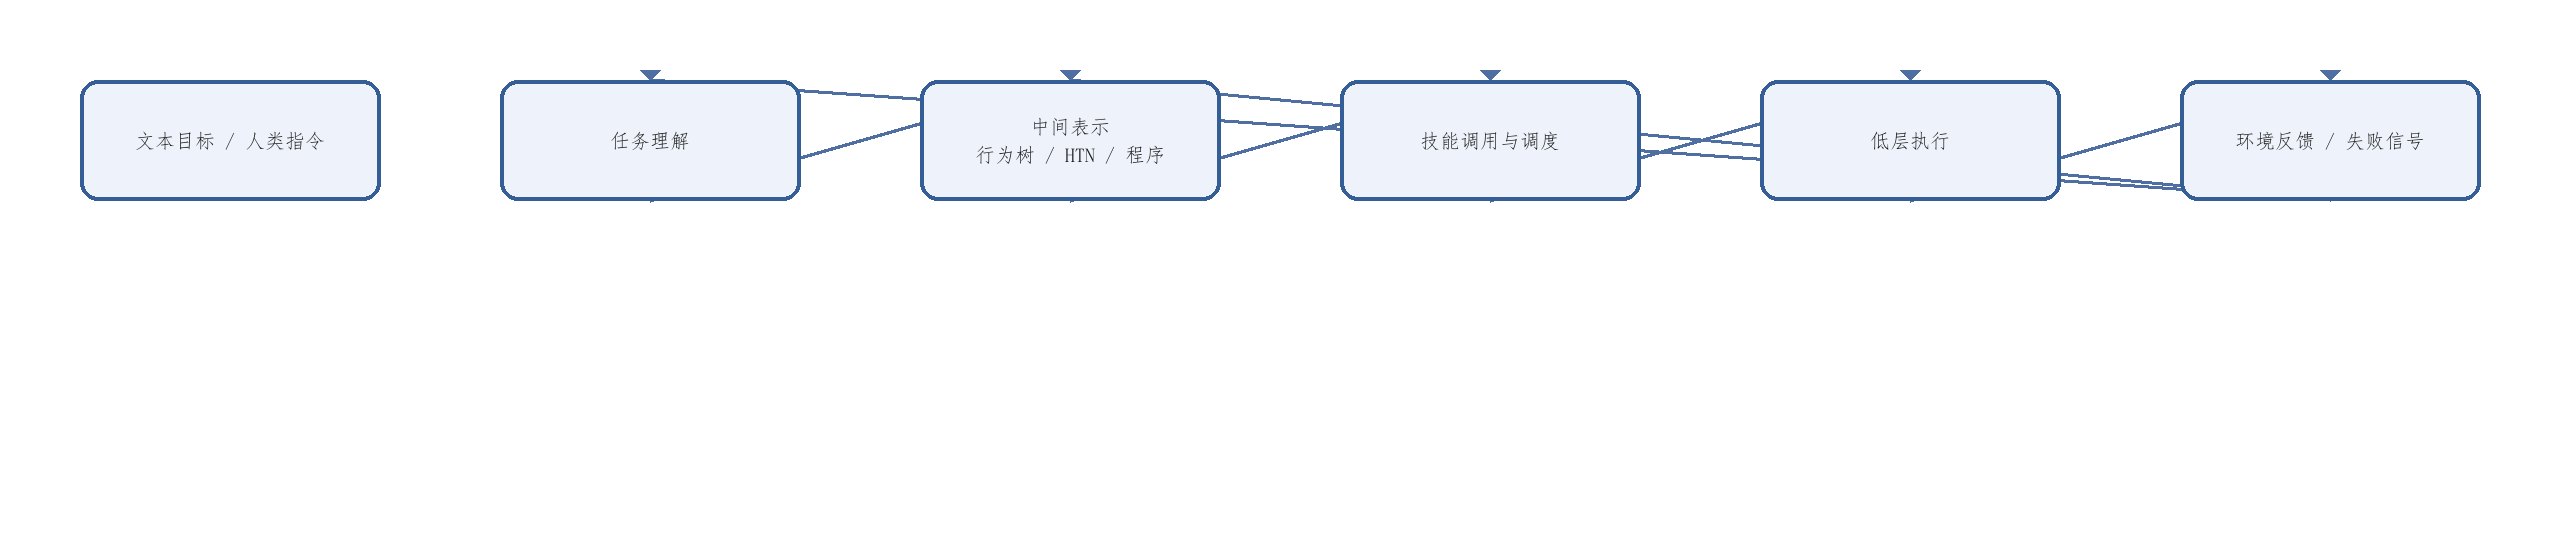
\includegraphics[width=0.9\textwidth,height=0.72\textheight,keepaspectratio]{figures/12-规划执行接口图.png}
\caption{12-规划执行接口图}
\label{fig:12-规划执行接口图}
\end{figure}

在当前版本中，\texttt{\detokenize{图 12-1 规划到执行的接口图}} 已承担“文本目标 -> 中间表示 -> 技能调用 -> 执行反馈”的主流程说明；\path{表 12-1 行为树 / HTN / 程序化中间表示比较表} 则把三类中间表示的表达能力、可验证性、回退机制与工程维护成本稳定为正式对照口径。

\section*{表 12-1 行为树 / HTN / 程序化中间表示比较表}
\addcontentsline{toc}{chapter}{表 12-1 行为树 / HTN / 程序化中间表示比较表}
\markboth{表 12-1 行为树 / HTN / 程序化中间表示比较表}{表 12-1 行为树 / HTN / 程序化中间表示比较表}

\begingroup
\small
\begin{xltabular}{\textwidth}{YYYY}
\toprule
维度 & 行为树（Behavior Tree） & HTN（Hierarchical Task Network） & 程序化中间表示（Code/Program-like IR） \\
\midrule
\endfirsthead
\toprule
维度 & 行为树（Behavior Tree） & HTN（Hierarchical Task Network） & 程序化中间表示（Code/Program-like IR） \\
\midrule
\endhead
核心思想 & 用节点组合执行、回退与条件判断 & 先给任务分层，再逐步细化子任务 & 用代码式结构表达任务、条件、调用与异常 \\
优势 & 执行流清晰、回退机制直观、工业可维护性强 & 任务结构表达能力强，适合长程分解 & 表达灵活，可与工具调用、API、内存检索结合 \\
弱点 & 高层语义表达有限，复杂任务易膨胀 & 维护复杂，依赖任务分解先验 & 易引入自由度过高、验证困难和隐藏异常分支 \\
可验证性 & 高 & 中到高 & 依赖约束方式，差异大 \\
回退与恢复 & 强，天然支持 fallback / retry & 可设计，但通常更依赖规划器逻辑 & 取决于运行时与异常处理设计 \\
与大模型结合方式 & 大模型生成或修订树结构 & 大模型负责高层分解或补齐缺失步骤 & 大模型直接生成程序、函数调用图或 DSL \\
对执行器接口要求 & 中 & 中 & 高，常需更严格运行时沙箱与检查器 \\
适用场景 & 重复性流程、工业任务、稳定工艺链 & 多阶段任务、任务层级清晰的复杂流程 & 需要开放工具、知识调用、临时组合能力的任务 \\
主要风险 & 树规模膨胀、节点维护成本高 & 分解错误会层层传递 & 生成自由度高，易出现不可控分支 \\
\bottomrule
\end{xltabular}
\endgroup

从后续维护方法上看，新增规划类工作时，建议先查 规划与具身推理论文清单，再进入对应单篇论文卡或正文补写。

\input{chapters/13-数据工程与训练闭环}
\input{chapters/14-仿真、数字孪生与评测基础设施}
% Generated from 15-机器人硬件、系统集成与部署约束.md; edit the LaTeX source after migration.

\reportpart{第十五部分 机器人硬件、系统集成与部署约束}
\addcontentsline{toc}{part}{第十五部分 机器人硬件、系统集成与部署约束}
\markboth{第十五部分 机器人硬件、系统集成与部署约束}{第十五部分 机器人硬件、系统集成与部署约束}

具身智能最容易被低估的一件事，是模型能力与可部署系统之间还隔着一整层硬件和系统工程现实。许多公开演示看起来讨论的是“大脑是否足够聪明”，但真正决定系统是否能进入工厂、仓库、楼宇、医院或家庭的，往往是机械结构是否可制造、执行器是否可靠、传感器链路是否稳定、算力与散热是否可承受、软件中间件是否易于维护、现场运维是否可持续。因此，本部分讨论的不是“机器人硬件简介”，而是为什么硬件路线与系统集成方式会直接决定现代具身系统的上限。

一个有代表性的现实信号是：近年的具身系统越来越不是“单模型论文”，而是“本体 + 端侧算力 + 传感器栈 + 中间件 + 运维链路”的整体方案。NVIDIA Jetson/Isaac 体系明确把嵌入式算力、ROS 加速栈、仿真、训练和部署放在同一产品叙事中；Figure Helix 也明确公开了其双系统、双嵌入式 GPU 的机载部署结构。这些材料说明，到了具身系统落地层，模型能力从来不能脱离硬件预算和系统集成方式独立讨论。\href{https://www.nvidia.com/en-us/autonomous-machines/embedded-systems/jetson-orin/}{Jetson Orin}、\href{https://www.figure.ai/news/helix}{Figure Helix}

\section*{71. 机器人本体硬件路线}
\addcontentsline{toc}{chapter}{71. 机器人本体硬件路线}
\markboth{71. 机器人本体硬件路线}{71. 机器人本体硬件路线}

\subsection*{71.1 机械结构设计}
\addcontentsline{toc}{section}{71.1 机械结构设计}


机械结构设计不只是工业设计问题，而是算法路线的前提条件。连杆布局、自由度分配、刚度、重量分布和可达工作空间，会直接决定感知盲区、控制难度、动作库设计和可执行任务集合。很多所谓“通用智能”在换一个本体后失效，根源并不在模型，而在原先默认的机械条件消失了。

因此，本体结构不应被视作算法之外的外部变量，而应被视作具身系统共同定义问题空间的一部分。谁忽略这一点，谁就会系统性高估模型迁移能力。

同样的“任务成功率”在不同本体上往往并不具有可比性，因为本体结构本身决定了感知盲区、可达姿态集合、接触方式和稳定性边界。也正因此，算法评测若脱离本体约束，很容易夸大跨平台结论。对长期跟踪行业的人来说，阅读系统进展时必须先问“这个能力建立在哪种本体假设上”，再问“这个能力是否可迁移”。

机械结构不是“承载模型的壳”，而是决定可达空间、负载边界、刚柔特性、维护难度和制造成本的第一性对象。人形、双臂、四足、移动操作平台和固定机械臂之所以在系统能力与商业路径上差异巨大，根本上就是因为机械结构决定了问题空间本身。

这也意味着机械结构不是中性容器，而是问题定义器。自由度数目、连杆长度、底盘形式、重心布局和工作空间会直接改变感知、规划与控制的难度分布，因此“算法能力”永远是在具体本体上成立的局部结论，而不是漂浮在硬件之外的抽象属性。

\subsection*{71.2 执行器与关节设计}
\addcontentsline{toc}{section}{71.2 执行器与关节设计}


执行器与关节设计决定的，不只是最大速度和最大力矩，还决定控制带宽、柔顺性、热管理、噪声、寿命与维护周期。这些因素会反过来限制高层策略能否被稳定兑现。例如一个在仿真里看起来简单的快速纠偏动作，在真实执行器上可能因为延迟、背隙或热限制而不可行。

因此，执行器选择本质上也是智能设计。它决定了系统可以在哪种时间尺度上做闭环，能否承受高频微调，以及错误发生后有多大恢复余地。

执行器路线决定了功率密度、背驱性、控制带宽、热管理和能耗。一个“会规划”的系统，如果执行器热崩溃、减速器寿命不足或关节响应过慢，就不可能稳定部署。

对具身系统尤其要强调一点：算法往往默认动作空间可以被可靠执行，但真实执行器并不会无条件满足这种假设。带宽不够时，高层输出再合理也会在低层变成滞后动作；背驱性差时，接触操作与人机协作的安全性会显著下降；热管理差时，系统在短时演示中可以工作，却无法支撑长时运行。执行器并不是被动“把动作做出来”的末端元件，而是在反向定义算法究竟能假设怎样的控制世界。 从系统弹性角度看，执行器也决定了模型误差可被吸收多少。高带宽、低回差、热余量足够的执行器，能够容忍上层策略一定程度的粗糙性；反之，任何一点动作抖动或时延都会迅速转化为振荡、打滑或能耗异常。因此，执行器选型常常直接决定系统对大模型不确定性的容忍边界。

这也是为什么很多“算法换代”最终会回到执行器现实：如果硬件本身无法稳定兑现高层动作意图，那么更复杂的策略往往只是在把误差更快地下传。对具身系统而言，执行器能力不是背景常量，而是高层智能能否真正落地的增益上限。

\subsection*{71.3 末端执行器与灵巧手}
\addcontentsline{toc}{section}{71.3 末端执行器与灵巧手}


末端执行器与灵巧手决定的，不只是“能不能抓”，而是“以什么方式抓、允许多大误差抓、抓错后能否恢复”。两指夹爪、吸盘、软夹爪、多指灵巧手和专用工装并不是同一问题上的不同参数，而是不同操作哲学。前者更强调低成本、强约束和高可靠，后者更强调姿态自由度、接触调节和潜在通用性，但也伴随更高控制与维护复杂度。

因此，末端选择不应只按“自由度越高越先进”来判断。很多高价值落地场景真正需要的不是最灵巧的手，而是最稳定、最便宜、最容易维护、最容易被客户接受的执行器组合。灵巧手更像是在扩大任务边界，而夹爪与工装更像是在压缩任务不确定性；谁更优，取决于公司是在争取短期交付还是长期通用能力上限。 末端执行器与灵巧手决定的，不只是“能不能抓”，而是“以什么方式抓、允许多大误差抓、抓错后能否恢复”。两指夹爪、吸盘、软夹爪、多指灵巧手和专用工装并不是同一问题上的不同参数，而是不同操作哲学。前者更强调低成本、强约束和高可靠，后者更强调姿态自由度、接触调节和潜在通用性，但也伴随更高控制与维护复杂度。

因此，末端执行器的选择本质上是在决定算法要面对什么难度等级。很多看起来“智能更强”的系统，只是因为它被允许使用更简单、更强结构化的末端工具；反过来，一旦换成通用灵巧手，感知、接触建模和控制难度都会同步上升。这也是为什么本报告始终把“本体工具链”与“算法路线”放在一起讨论。

末端执行器之所以关键，是因为它是语义计划第一次真正接触物理世界的地方。高层模型可以正确判断“应该拿起杯子”，但如果抓手开合范围、接触材料、指尖摩擦和力控精度不匹配，整个系统仍会在最后一厘米失败。很多所谓“模型问题”最终其实是末端执行器适配不足的问题，只是这个问题在论文叙事里常被高层模型光环掩盖。

很多具身系统最终卡住的地方，并不是“不会理解任务”，而是末端执行器不够适配、灵巧手不够稳、抓取策略无法覆盖长尾对象。也就是说，硬件接口和动作能力边界在末端最直接暴露出来。 灵巧手尤其体现这种张力。它一方面显著提升了操作上限，使旋拧、重抓、双指拨动、复杂接触调整等任务成为可能；另一方面也把控制、校准、磨损、故障诊断和数据采集复杂度大幅抬高。灵巧手因此常常是“能力上限”和“工程复杂度”之间最剧烈的摇摆点。

\subsection*{71.4 本体差异为什么会反过来改写算法路线}
\addcontentsline{toc}{section}{71.4 本体差异为什么会反过来改写算法路线}


本体差异会改写算法路线，是因为智能从来不是悬浮在身体之上的。不同本体拥有不同的观测方式、接触模式、约束集合和失败后果，因此同一种学习与规划方法在不同本体上往往对应完全不同的有效性边界。轮式移动平台、人形、固定臂和双臂系统并不是在同一问题上做同一件事。

从系统角度看，本体其实决定了“最容易把什么做对、最容易把什么做错”。固定臂更容易把感知视角、工作空间和接触条件稳定下来，因此算法可以更依赖示教、重复和局部精调；人形或移动操作系统则要同时面对平衡、导航、遮挡、接触和长链条恢复，导致状态空间和失败模式一起爆炸。于是算法路线也不得不更强调分层决策、局部安全冗余和可恢复执行，而不是只追求单次动作最优。

这也解释了为什么某条在特定本体上表现亮眼的路线，并不应自动被翻译成“通用更先进”。很多时候，算法成绩的一部分其实来自本体给出的强先验，例如吸盘末端把抓取问题压缩成吸附判定，或固定相机布局把三维感知问题压缩成有限视角识别。比较模型时若忽略这些身体条件，就很容易把“本体优势”误读成“算法优势”。

这意味着算法比较若不注明本体条件，就很容易失真。很多路线看似“更强”，只是因为它依赖了更友好的身体假设。报告后续比较企业和论文时，应持续保留这种本体敏感性。

这也是为什么很多真正成熟的系统路线，最后都会回到“平台定制化通用性”而非抽象的一体化通用性。也就是说，模型可以共享上层语义与部分技能结构，但很少能完全无视本体差异地共享整条执行链。谁忽视这一点，谁就容易高估跨平台预训练或通用策略接口的直接可迁移性。

同一套算法在固定臂、移动操作平台和人形上往往表现完全不同，根源并不只是数据集差异，而是动作空间维度、视角耦合、稳定性边界和接触几何都被本体改写了。因此，“通用具身模型”如果不把本体差异纳入设计变量，就容易把平台间迁移难度说得过于轻松。 因此，不存在脱离本体的“最佳算法”。同样的数据组织方式、动作表示和接口抽象，在不同本体上可能需要完全不同的技能切分、安全边界和评估指标；真正成熟的系统路线通常不是忽略本体，而是显式承认本体会反过来重写算法问题本身。

\section*{72. 传感器与板载计算}
\addcontentsline{toc}{chapter}{72. 传感器与板载计算}
\markboth{72. 传感器与板载计算}{72. 传感器与板载计算}

\subsection*{72.1 相机、IMU、力觉、触觉}
\addcontentsline{toc}{section}{72.1 相机、IMU、力觉、触觉}


这些传感器之所以必须并列讨论，是因为它们分别对应不同时间尺度和不同类型的不确定性。相机更擅长提供远距离、全局、语义化信息，\texttt{\detokenize{IMU}} 更适合快速姿态与加速度估计；力觉与触觉则在接触发生后提供视觉难以替代的局部状态反馈。系统是否真正具备闭环韧性，很大程度上就取决于它能否在这些信号之间完成有效分工。

也正因此，传感器设计不是“多多益善”的堆料问题，而是信息职责划分问题。若视觉已经足以完成远场定位，就未必需要再让它承担细粒度接触判断；若触觉只能在接触后工作，就不能把避碰责任完全压给触觉层。成熟系统往往先明确每类传感器在何时最可信、何时只是辅助信号，再围绕这种可信度结构来设计融合与回退逻辑。 这些传感器之所以必须并列讨论，是因为它们分别对应不同时间尺度和不同类型的不确定性。相机更擅长提供远距离、全局、语义化信息；IMU 更适合快速姿态与加速度估计；力觉与触觉则在接触发生后提供视觉难以替代的局部状态反馈。系统是否真正具备闭环韧性，很大程度上就取决于它能否在这些信号之间完成有效分工。

更进一步说，传感器选择并不是“越多越好”。每增加一种模态，就会增加标定、同步、带宽、噪声建模和维护成本。真正成熟的系统会围绕任务需要决定最关键的观测变量，而不是无差别堆叠传感器。对学习者而言，这一点很重要，因为它能避免把多模态误读为天然先进。

传感器栈设计不是越多越好，而是必须围绕任务链路决定：哪些状态必须高频可见，哪些观测必须低延迟，哪些冗余是为了安全，哪些信号只是为了离线调试。

在很多失败部署中，问题并不出在传感器“数量不足”，而出在职责不清。例如，相机同时承担高层识别、局部避障、接触前精定位和失败诊断，结果任何一个链路的时延或失焦都会拖垮整条系统。更合理的传感器分工通常是：视觉负责较丰富但相对慢的远距语义，IMU 与编码器负责高频本体状态，力觉和触觉在接触阶段接管关键反馈。 成熟传感栈的标志，不是堆更多模态，而是职责边界清楚。相机负责远距语义和几何，IMU 与编码器承担高频状态估计，力觉与触觉服务接触闭环，日志与回放系统负责事后诊断；只有在这种明确分工下，多模态融合才会从“信息更多”变成“系统更稳”。

\subsection*{72.2 算力、功耗与散热}
\addcontentsline{toc}{section}{72.2 算力、功耗与散热}


算力、功耗与散热之所以要放在同一个小节，是因为它们在真实机器人上几乎从来不是彼此独立的变量。更大的模型往往意味着更高的推理吞吐需求，更高吞吐又意味着更高功耗，而更高功耗最终会转化为散热、续航、体积和结构设计压力。于是，“能不能部署某个模型”常常首先不是算法问题，而是热设计与能源预算问题。

若把这层约束写得足够朴素，可以近似理解为：

\begingroup
\footnotesize
\begin{equation*}
\text{deployable model} \subseteq \{\text{latency}, \text{power}, \text{thermal budget}\}
\end{equation*}
\endgroup

也就是说，一个模型即便精度更高，只要超过现场功耗或散热预算，就未必是更优系统选择。

大模型进入机器人之后，算力与能耗问题被显著放大。端侧算力不够，推理时延会上升；算力太强，散热和电源设计又成为瓶颈。于是，“模型能不能跑”在机器人里从来不是软件问题，而是功耗-体积-续航-散热共同约束的问题。Jetson Orin 官方页面给出的产品线信息就很能说明这种现实：同一代模块需要在 10W 到 60W 甚至更高的性能-功耗区间内做取舍，而不同部署平台能接受的热设计空间完全不同。\href{https://www.nvidia.com/en-us/autonomous-machines/embedded-systems/jetson-orin/}{Jetson Orin} 算力、功耗与散热因此不是部署后的收尾工作，而是模型设计阶段就必须前置考虑的约束。一个在实验台上依靠高风量散热、外接供电和短时推理才能工作的模型，往往并不自动等价于可机载、可移动、可长时运行的系统能力；很多“模型选型”实际上都是热预算与续航预算上的系统取舍。

如果把 \href{https://www.nvidia.com/en-us/autonomous-machines/embedded-systems/jetson-orin/}{Jetson Orin} 的公开口径进一步拆开看，会更容易理解为什么端侧模型路线一定要重写。NVIDIA 在官方页面里把同代模块明确划成从 \texttt{\detokenize{Jetson Orin Nano}} 到 \texttt{\detokenize{Jetson AGX Orin}} 的多个功耗-性能档位，覆盖大致 \texttt{\detokenize{7W-60W}} 的部署区间与 \texttt{\detokenize{67 TOPS-275 TOPS}} 的 AI 性能范围。这意味着“同样叫端侧 GPU”在机器人里其实对应完全不同的热设计、供电、机身空间和风道设计条件。对研究者而言，真正有价值的不是背下某个 TOPS 数字，而是意识到：模型结构、上下文长度、输入帧率和动作刷新频率一旦改变，整个热-功耗-时延预算都会被联动改写。

也因此，算力预算最忌讳的误判是把“单次推理速度够快”误认为“系统长期可运行”。对机器人来说，更关键的通常是峰值负载下的稳定帧率、长时间运行时的温升曲线、推理线程与控制线程的争用关系，以及热降频是否会把原本看似满足闭环的模型拖回超时区间。许多路线在实验桌面上成立，却在移动平台或紧凑人形本体上迅速变脆，本质上就是因为它们从一开始就没有把热与功耗视为能力定义的一部分。

更进一步说，机器人里的“算力预算”从来不是单独给模型的预算，而是与执行器、传感器和冷却系统争抢同一整机资源池。若本体已经需要大量功率维持运动、抓取和安全冗余，那么留给模型和散热的空间就天然更窄。这也是为什么同样的 VLA 路线，落在固定双臂、移动操作平台和人形本体上会得出完全不同的最优模型规模与刷新频率。算法不是在抽象显卡上运行，而是在具体机电系统里争取自己的那部分能量与散热额度。

因此，这一节最该建立的工程直觉是：模型结构、上下文窗口、输入分辨率和动作刷新率都必须被翻译成持续功耗与持续热负荷，而不是只被翻译成 benchmark 分数。谁忽略这一步，谁就会高估“大模型直接上本体”的成熟度。

\subsection*{72.3 通信与同步}
\addcontentsline{toc}{section}{72.3 通信与同步}


通信与同步看起来像中间件细节，实际上是很多具身系统成败的隐性分水岭。感知、状态估计、规划、控制和日志记录若不在同一时间轴上对齐，系统就会在高层看似合理、底层却持续失配。尤其在多相机、多关节、多计算节点和远程监控同时存在时，毫秒级偏差都可能被接触任务放大成失败。

因此，同步不是后台工程问题，而是控制正确性的一部分。一个模型若在离线回放里表现很好，真机却总在接触前后出错，根源有时不是策略不行，而是数据与控制链路时钟不一致。后续报告涉及系统案例时，应持续注意这一类“看不见但决定闭环”的因素。

从系统工程角度看，很多“模型偶发失灵”最后都会被追溯为通信拥塞、消息延迟抖动、同步漂移或队列堆积问题。机器人系统之所以难维护，正是因为这些问题在短演示中不一定出现，却会在长时运行中积累成结构性故障。也因此，时间同步和通信质量不应被视为基础设施细节，而应被视为闭环能力的一部分。

多传感器、多控制器和云边端协同时，通信链路与时间同步本身就是能力边界。一个感知模型再强，如果跨模块时间戳混乱，闭环控制仍然会出问题。 这类问题之所以危险，在于它们经常以“偶发不稳”“难以复现”“看似像模型退化”的形式出现。实际上一旦观测、状态和动作流的时间基准错位，任何高层智能都会被底层不一致性侵蚀。因此，同步与通信不是底层洁癖，而是系统可诊断性、可维护性和可验证性的基础。

从部署视角看，同步问题最糟糕的地方在于它往往不会立刻表现为彻底失效，而是表现为难以定位的概率性退化。也正因此，成熟系统通常会把时间戳一致性、消息延迟统计、队列积压监控和回放一致性检查纳入默认运维工具链，而不是等故障出现后再临时排查。

把这个问题写得更形式化一点，可以把某一控制决策真正依赖的观测有效年龄记成：

\begingroup
\footnotesize
\begin{equation*}
\Delta t_{\text{obs}} = t_{\text{apply}} - t_{\text{sense}}
\end{equation*}
\endgroup

只要 \(\Delta t_{\text{obs}}\) 在运行中大幅抖动，即使平均值不高，系统也可能在接触、平衡或协作任务中迅速失稳。这个表达式的重要性在于，它提醒我们通信与同步问题并不是抽象“系统工程噪声”，而是直接改变闭环中每一个控制决策究竟在看多旧的数据。

也正因此，通信设计的重点不只是带宽，更是消息优先级、QoS 语义、队列策略和时钟一致性。一个成熟的机器人软件栈必须能回答：哪些消息可丢、哪些必须保序、哪些允许历史滞后、哪些超过时限就必须触发安全回退。若这套语义没有被写清，“模型接上总线”就只是把智能接进了一个不稳定时钟系统。

\subsection*{72.4 端侧算力预算如何约束模型}
\addcontentsline{toc}{section}{72.4 端侧算力预算如何约束模型}


端侧算力预算并不只是“模型能不能跑起来”的问题，而是直接决定系统可以拥有什么样的时间结构。若推理延时太高，系统就必须减少决策频率、增大动作 chunk、或把更多职责下放给传统控制器；若功耗和散热压力太大，模型即便在短时演示中可跑，也可能在长时间现场运行中不可持续。于是算力预算会反过来改写动作表示、调度策略和安全回退设计。

这意味着端侧算力不是部署阶段才考虑的约束，而应在模型设计初期就进入问题定义。一个离线很强、在线很慢的模型，并不只是“部署还要优化”，而可能从一开始就没有回答真实机器人闭环最关键的时间问题。 端侧算力预算的约束方式非常直接：它会同时决定可接受的模型规模、上下文长度、感知刷新频率和安全冗余策略。若算力预算不足，系统往往必须在“更高精度的单次推理”和“更高刷新率、更低时延的连续闭环”之间做取舍。

一个最小预算判断可以写成：

\begin{lstlisting}[language=python]
if model_latency > control_deadline:
    use_smaller_model_or_chunked_policy()
\end{lstlisting}

这说明端侧算力预算不是部署后才考虑的小问题，而是会反过来塑造动作表示、架构分层和推理频率设计。

因此，端侧模型选择本质上是系统级预算分配问题，而不是单独的算法偏好问题。更大的模型可能提升语义理解，却也可能挤压续航、散热和执行稳定性预算；很多时候，部署上的最优解并不是“最准的模型”，而是“在预算内整体效果最稳的模型”。

若把部署预算极简化地写成：

\begingroup
\scriptsize
\begin{equation*}
P_{\text{total}} = P_{\text{compute}} + P_{\text{actuation}} + P_{\text{sensing}} + P_{\text{cooling}}
\end{equation*}
\endgroup

那么很多“为什么不用更大的模型”的答案其实都藏在这个等式里。对机器人而言，\(P_{\text{actuation}}\) 与 \(P_{\text{sensing}}\) 经常已经占用很大份额，留给 \(P_{\text{compute}}\) 与 \(P_{\text{cooling}}\) 的空间远比数据中心推理小得多。

\section*{73. 软件栈与中间件}
\addcontentsline{toc}{chapter}{73. 软件栈与中间件}
\markboth{73. 软件栈与中间件}{73. 软件栈与中间件}

\subsection*{73.1 ROS/ROS 2}
\addcontentsline{toc}{section}{73.1 ROS/ROS 2}


ROS/ROS 2 的意义，不只在于提供通信中间件，更在于它们长期充当了机器人系统模块化组织的事实标准。消息接口、节点划分、工具链生态和调试方式，都会通过这套框架影响团队如何设计系统边界。即使某些商业系统不会完整沿用 ROS，也常常在概念与工程习惯上受到它深刻影响。

因此，理解 ROS/ROS 2 的价值，不应只停留在“会不会用工具”，而要看到它们如何塑造了机器人系统的组织方式，以及为什么具身系统即便引入更强学习模块，也依旧需要稳定中间件层。

对报告读者而言，理解 ROS/ROS 2 的价值不应停留在“会不会用工具”，而应上升到“为什么机器人需要稳定的软件总线”。一旦感知、规划、控制、日志、监控和运维都要长期协作，中间件就不再只是开发便利性问题，而是系统可维护性问题。很多企业路线看似在“卷模型”，实则大量工程差异都积累在消息流、状态机和调试链路中。

ROS/ROS 2 的长期重要性，并不在于它们是“最新框架”，而在于它们提供了模块通信、消息抽象、调试和生态整合的事实标准接口。很多系统即使高层模型完全不同，底层工程仍然会在某种程度上依赖类似中间件结构。 更准确地说，ROS/ROS 2 的价值不仅在工具生态，而在于它们为“模块如何通信、状态如何暴露、日志如何回放、问题如何定位”提供了公共回答。对长期演进的具身系统而言，这种公共回答会直接影响团队协作效率、故障排查成本和后续模型替换的摩擦。

从 \href{https://github.com/ros2/ros2}{ROS 2 官方仓库} 的定位也能看出这一点。它并不是单个消息库，而是一组围绕节点通信、消息接口、开发工具和中间件适配共同演化的软件集合。对具身系统而言，这意味着 ROS 2 的真正价值从来不只是“能发消息”，而是它帮团队把哪些状态必须显式暴露、哪些模块必须可回放、哪些节点可以被替换、哪些异常需要被记录，慢慢固定成了一种事实工程文化。后续即便有团队不用原生 ROS 2，也往往还会延续这种“中间件先定义系统边界”的思维方式。

\subsection*{73.2 实时控制系统}
\addcontentsline{toc}{section}{73.2 实时控制系统}


实时控制系统的职责，并不是简单地“把命令发快一点”，而是为整个具身系统提供可预测的局部稳定基础。高层模型可以偶尔犯错并被回退，但底层控制若无法稳定守住频率、抖动和安全边界，那么所有上层能力都会被瞬间放大为物理风险。也正因此，很多看似不够“AI”的实时控制栈，反而构成了整套系统最不可替代的安全骨架。

从工程组织角度看，实时控制系统还承担版本隔离作用。它让上层模型、规划和任务接口可以更快试错，同时尽量避免每次模型更新都直接冲击最敏感的物理回路。没有这层隔离，研发速度和部署安全往往会彼此拖累。 实时控制系统的核心不是“运行得快”，而是“在确定的时间预算内稳定运行”。机器人控制最怕的并不是平均时延略高，而是抖动过大、最坏情况不可控。一次偶发的调度延迟、缓存阻塞或线程抢占，就可能让本来稳定的接触与平衡任务突然失效。

因此，实时控制系统应被理解为对时间一致性的工程承诺。它要求软件架构、操作系统、线程调度、总线通信和安全机制共同围绕最坏情况约束设计，而不只是围绕平均性能优化。这一点也是很多 AI 团队进入机器人后最容易低估的现实门槛。

机器人一旦进入毫秒级控制，就必须面对一般 AI 软件系统很少处理的实时性要求。调度抖动、线程优先级、控制器循环时间和硬件驱动稳定性，都会直接决定系统是否可用。

这里的困难在于，大模型与现代推理栈天然不是为硬实时设计的。它们喜欢批处理、容忍推理波动、追求平均吞吐；而机器人控制往往宁可牺牲一点平均性能，也要保障最坏时延上界。因此，真实系统通常不得不把高层推理、技能执行、控制环和安全监控拆到不同频率域和不同优先级上运行。 这也是 ROS 2、DDS QoS、实时 Linux 与本地 watchdog 机制在具身系统中长期重要的原因。它们并不是“老派工程细节”，而是把概率性 AI 输出装进确定性控制系统的必要胶水，相关系统文档可参见 \href{https://docs.ros.org/en/rolling/index.html}{ROS 2 文档}。

如果把这一点和当前企业公开架构放在一起看，会更清楚为什么“基础模型不可能直接承担全部实时责任”。\href{https://www.figure.ai/news/helix}{Figure Helix} 明确公开了 \texttt{\detokenize{S2}} 以 \texttt{\detokenize{7-9 Hz}} 更新高层语义、\texttt{\detokenize{S1}} 以 \texttt{\detokenize{200 Hz}} 维持低层控制的分层结构；这与实时系统设计逻辑完全一致，即让语义模型服务于阶段决策与目标更新，而把真正需要硬时间保证的闭环留在更轻、更近、更确定的控制层里。也正因为如此，具身系统里最成熟的路线往往不是“让模型更像控制器”，而是“让控制器与模型之间的责任边界更清楚”。

这个例子很重要，因为它说明“高层模型刷新慢”并不天然意味着系统弱，关键在于刷新慢的那一层到底承担什么责任。若它只负责阶段切换、目标更新和语义解释，那么 \texttt{\detokenize{7-9 Hz}} 甚至更慢都可能足够；若它试图直接承担接触稳定、姿态保持和轨迹跟踪，那么同样的频率就会明显失效。实时系统设计真正做的，不是追求所有模块都更快，而是按责任把不同模块放进不同的时间预算里。

因此，实时控制层在具身系统中的价值，不是与大模型竞争“谁更聪明”，而是替整套系统守住“谁必须确定”这条底线。只要这一底线还存在，实时控制层就不会被大模型直接替代。

\subsection*{73.3 感知、规划、控制的模块协同}
\addcontentsline{toc}{section}{73.3 感知、规划、控制的模块协同}


模块协同真正难的地方，不在于“模块之间能不能通信”，而在于它们是否共享一致的时间轴、状态定义和异常语义。感知认为目标已经对准、规划认为路径仍安全、控制却检测到接触异常，这类跨模块认知冲突若没有统一解释机制，就会在现场不断演化成难以复现的失败。

因此，协同设计的关键往往是中间合同而不是算法本身。每个模块必须明确自己输出的置信度、适用边界、终止条件和异常上报方式。只有这样，系统才不是单纯把多个强模块串起来，而是真正形成可诊断、可回放、可回退的整体。

感知、规划、控制的模块协同问题，表面上看像系统集成细节，实际上往往决定整机是否能稳定工作。感知输出若延迟或不稳定，规划层就会建立在过时状态之上；规划层若给出的目标不可执行，控制层就只能不断做保守补偿；控制层若无法把异常及时反馈回来，高层又会持续基于错误假设做后续决策。

因此，系统协同的关键不只是模块都“各自够强”，而是模块之间是否在时间尺度、接口语义和异常处理上形成闭环。很多部署失败并不是由单个算法模块能力不足造成，而是由模块之间的弱错配长期积累出来的。

模块协同难，不只是因为模块多，而是因为每个模块都在不同时间尺度上工作且互相依赖。感知误差会改变规划可行域，规划延迟会改变控制稳定区间，控制抖动又会反过来污染感知输入，这种闭环耦合是软件系统里少见而在机器人里极常见的复杂性来源。真正的系统集成能力，往往体现在能否把这些耦合控制在可诊断、可回退的边界内。

系统集成真正困难的地方，是这些模块不是串行调用关系，而是一个持续相互影响的闭环。很多实验室系统之所以难以转为产品，并不是因为单模块不够强，而是跨模块耦合、异常传播和调试成本过高。

\subsection*{73.4 “模型接 ROS”并不等于系统集成完成}
\addcontentsline{toc}{section}{73.4 “模型接 ROS”并不等于系统集成完成}


把模型接进 ROS 或 ROS 2，只意味着它进入了消息总线，并不意味着它已经成为可用系统的一部分。真正的系统集成还需要解决消息频率匹配、时间同步、异常处理、节点重启、状态回传、权限边界和安全回退策略。也就是说，“能收到图像、能发出动作”只是集成的起点，而不是终点。

一个最小集成链路通常至少包含：

\begin{enumerate}
\item 感知消息订阅与时间戳对齐。
\item 模型推理服务或节点封装。
\item 动作输出与控制接口适配。
\item 失败监控、回退策略与日志记录。
\end{enumerate}

这是具身系统里非常常见的误解。把一个视觉模型或策略模型挂到 ROS topic 上，只说明接口打通了；但真正的系统集成还包括时间同步、故障传播控制、日志回放、状态机回退、安全栅栏与现场维护工具。也正因为如此，工程团队常常把大量时间花在“模型之外”的中间件调试上。

如果把系统集成理解成“把 AI 模型挂到现有机器人软件上”，就会系统性低估大量非算法工作。真正让系统可交付的，往往是那些不显眼但决定稳定性的细节：例如图像与本体状态是否严格对齐、多个节点之间的 QoS 配置是否合理、推理超时是否触发安全停机、上游感知缺帧时下游控制是否继续输出旧命令、模型升级后回归测试是否覆盖历史失败案例。

因此，这一节最应该建立的观念是：模型只占系统中的一个节点，而产品级机器人需要的是一条“可观测、可诊断、可回退、可恢复”的执行链。很多 demo 能跑，是因为操作者在旁边手动兜底；很多产品跑不稳，则是因为系统把人的临场判断误当成了软件架构的一部分。

从交付视角看，真正的系统集成至少要把五类契约固定下来：输入契约、时间契约、异常契约、权限契约和回放契约。输入契约回答模型到底读哪些字段；时间契约回答这些字段允许多旧；异常契约回答上游失真时谁负责停；权限契约回答谁拥有最终否决权；回放契约回答事后能否重现当时状态。只要其中任意一项仍依赖口头经验而不是明确接口，系统集成就还没有完成。

\section*{74. 部署约束}
\addcontentsline{toc}{chapter}{74. 部署约束}
\markboth{74. 部署约束}{74. 部署约束}

\subsection*{74.1 实时性}
\addcontentsline{toc}{section}{74.1 实时性}


实时性在机器人语境里不是泛泛的“响应更快”，而是系统不同层在各自时间尺度上都必须满足可预测的更新周期。高层任务规划可以秒级刷新，局部动作策略可能需要几十毫秒，平衡与接触稳定则常常要求更高频率。若把这些层混在一起统一追求“更强模型”，就很容易牺牲掉真正关键的快回路。

一个有用的思考方式，是把闭环时延显式写成：

\begin{lstlisting}
T_total = T_sense + T_transport + T_infer + T_plan + T_act
\end{lstlisting}

若 \(T_total\) 超过该层闭环允许的时间窗口，那么再“聪明”的模型也只能在错误的时机做出正确判断。对抓取前姿态微调、双足平衡和接触稳定任务尤其如此，因为真正稀缺的能力往往不是语义推理，而是及时反应。

因此，成熟架构通常不会试图让同一个大模型承担所有频率层，而是清楚区分哪些决策值得耗时、哪些决策必须即时。慢但强的模型适合做语义解释、阶段切换和异常归因；快但窄的控制器则负责局部闭环。这种分工并不是妥协，而是物理系统对智能组织方式的基本要求。

所以，讨论实时性时最该追问的不是模型峰值能力，而是能力被放在了什么时间层里执行。谁能把快慢回路清楚分层，谁就更接近可部署系统；谁把一切都压进单一慢模型，谁就更容易在现实中失稳。

实时性之所以必须单列，是因为具身系统里很多失败并不是“决策错误”，而是“决策来晚了”。同样一个动作命令，早 50 毫秒和晚 50 毫秒抵达控制层，物理后果可能完全不同。因此，机器人里的性能优化不能只看平均吞吐与平均延时，更要看最坏时延上界与时延抖动。

闭环控制、障碍回避和接触调节都要求严格的时间预算。现实部署中，时延不只是性能下降源，更可能是安全风险源。 因此，实时性本质上也是资源伦理问题：哪些能力值得占用多少时间预算，哪些推理必须在超时后被硬切断，哪些判断必须让位给本地回退。一个模型的真正价值，不是离线精度有多高，而是在严格时间预算下还能保留多少有效能力。

\subsection*{74.2 可靠性}
\addcontentsline{toc}{section}{74.2 可靠性}


在机器人语境里，可靠性并不只是“平均成功率高”，而是“长时间运行时是否仍保持可预测行为”。这通常要求系统在传感器掉帧、网络抖动、对象轻微漂移、局部碰撞、模块重启和偶发异常下仍然不会迅速失控。

这里最需要防止的误判，是把 demo 成功率直接等价为系统可靠性。一次演示中的成功，往往只证明系统在某个狭窄条件下可以完成任务；而可靠性关心的是条件逐渐偏离、部件轻微老化、现场持续扰动后，系统会怎样退化。它是平滑降级、局部恢复，还是突然冻结、状态丢失、需要人工重启？这三种退化方式在产品意义上完全不同。

因此，更有信息量的可靠性指标通常包括 \texttt{\detokenize{MTBF}}、接管频率、平均恢复时间、误停机率和版本升级后的回归故障率。只有把这些信号与成功率放到一起，才能判断一个系统是否真的具备长期运转能力，而不是只具备“拍出一段成功视频”的能力。

因此，可靠性更适合被看作多层属性：

\begin{enumerate}
\item 模块可靠性：单个组件是否稳定。
\item 闭环可靠性：模块耦合后是否稳定。
\item 运维可靠性：长时间现场运行是否可恢复、可监控。
\end{enumerate}

机器人部署看的不是某次最好的成功率，而是长时间运行中的平均稳定性、故障间隔、可恢复性和维护可预测性。

在现场语境里，可靠性至少包含三层含义。第一层是动作可靠性，即单次操作是否稳定；第二层是系统可靠性，即连续运行数小时或数天后是否仍保持可接受表现；第三层是运维可靠性，即故障发生后是否能被快速诊断、回放、定位并恢复。很多研究系统在第一层表现不错，却在第二层和第三层几乎没有准备，因此无法真正跨过“研究演示”与“交付系统”之间的门槛。

\subsection*{74.3 成本与制造可行性}
\addcontentsline{toc}{section}{74.3 成本与制造可行性}


成本与制造可行性不是商业附录，而是技术路线的筛选器。一个系统若只能依赖高价执行器、复杂装配、高频人工校准和稀缺零部件，即使功能成立，也很难进入大规模复制阶段。很多研究路线的真正分水岭，不在实验室能否跑通，而在成本结构能否随着迭代收敛。

更准确地说，制造可行性讨论的不是“今天单台能不能做出来”，而是“明天一百台、一千台时会在哪里失控”。一旦规模上升，装配公差、标定一致性、返修率、备件通用性和供应链波动都会突然成为主问题。某些在实验室阶段看起来合理的技术选择，到了量产阶段可能因为良率太低、维护太重或关键零部件过于稀缺而失去意义。

这也是为什么成本结构本身会反过来约束算法与系统设计。若末端执行器太贵，系统就必须更强调抓取成功率与保护策略；若标定成本太高，模型与接口就必须更能吸收几何误差；若现场维护负担太重，架构就必须支持模块化更换、远程诊断和更强的本地回退。换言之，制造可行性不是部署后的附加考虑，而是从一开始就塑造技术上限的硬约束。

因此，本章更强调把 BOM、装配良率、标定工时、备件策略和维护周期一起纳入系统评价。谁能持续把这些变量压低，谁的技术路线才更可能成为产业路线，而不只是实验路线。

制造可行性会反过来塑造技术路线。若某类传感器、减速器或算力模组无法稳定供货，系统即使技术上可行，也难以形成持续交付能力，因此产业判断不能只看单台样机表现。很多路线之所以最终难以商业化，不是因为实验失败，而是因为无法跨过可制造性与供应链一致性这道门槛。

一个实验室系统即使能力强，如果 BOM 成本过高、制造良率不足、供应链不稳定，就很难形成大规模部署路径。 这里要看的也不只是 BOM。批量化要求一致性、工装夹具、校准流程、备件体系和维护培训一并可复制，否则样机成功并不能自然推导出规模化交付可行。因此，可制造性不是附加考量，而是从一开始就会重写系统设计的核心约束。

\subsection*{74.4 维护、升级与现场运维}
\addcontentsline{toc}{section}{74.4 维护、升级与现场运维}


很多具身系统在实验室里看起来接近完成，真正进入现场后却被运维问题重新打回原形。原因不在模型突然变差，而在现场世界要求系统面对备件更换、传感器漂移、版本回滚、网络中断、客户误操作和安全责任界面这些实验室里很少完整暴露的问题。维护能力因此不是售后附属项，而是产品能否持续存在的组成部分。

更成熟的运维体系通常会把问题分成三层：本地可自动恢复的问题、远程可诊断并修复的问题、以及必须人工现场介入的问题。谁能持续把更多故障从第三层压缩到前两层，谁就更接近可扩张交付。 维护、升级与现场运维经常被低估，因为它们在 demo 中几乎不可见，却在真实部署中持续吞噬成本。传感器清洁、关节磨损、线束老化、版本回滚、日志回收、备件更换和现场重新标定，都会随着部署规模扩大而迅速放大。一个短期能跑的系统，不等于一个长期可维护的系统。

因此，升级能力必须与回退能力同时设计，现场运维能力也必须被当作产品定义的一部分。谁只会“发布新版本”，却没有低风险升级和快速回滚机制，谁的部署规模越大，风险反而越高。

这意味着“可更新性”本身就是架构设计目标。日志能否回收、模型能否灰度升级、异常能否远程诊断、控制参数能否安全回滚，这些问题都会决定系统是不是只适合演示，而不是适合长期运行。对于具身系统而言，运维不是售后附属流程，而是能力闭环的一部分。

机器人不是一次性交付软件。传感器会老化、执行器会磨损、环境会变化、模型会过时，因此现场运维是能力的一部分，而不是售后附属品。 进入商业期后，运维往往会从“支持功能”变成主导变量。能否远程诊断、快速替换故障模块、灰度发布模型、回放历史异常、隔离问题版本，决定了系统究竟能不能活过大规模部署后的维护周期。

把现场运维写成更清楚的链条，可以近似分成：

\begin{lstlisting}
异常发现 -> 事件分级 -> 本地自恢复 / 远程诊断 / 现场介入 ->
日志回收 -> 根因定位 -> 热修复或版本回滚 -> 回归验证 -> 再放量
\end{lstlisting}

这个链条的价值在于，它把“运维”从笼统售后名词压回了系统生命周期。很多团队最初以为自己的难题是模型还不够强，后来才发现真正吞噬成本的是事件分级、日志回收、备件切换和安全升级流程。也因此，谁能把更多问题稳定压缩到“远程诊断 + 安全回滚”层，谁就更接近可规模化的产品能力。

\subsection*{74.5 成本模型与系统取舍}
\addcontentsline{toc}{section}{74.5 成本模型与系统取舍}


成本模型的意义，不只是解释“为什么现在贵”，而是帮助判断哪些技术选择会在规模化时越做越贵，哪些选择会随着迭代逐步收敛。某些路线在单机阶段看起来并不离谱，但只要一进入批量装配、跨客户部署和长期维护，隐藏成本就会快速显性化；另一些路线虽然前期研发重，但一旦接口稳定，后续复制成本会明显下降。

因此，系统取舍不应只按当前性能最优来做，而应同时问：这个选择会不会把未来的制造、标定、维护和升级成本一起锁死。很多“技术上最强”的方案之所以最终没成为主线，不是因为它不工作，而是因为它工作得太贵。

如果把单机交付成本粗略写成：

\begingroup
\scriptsize
\begin{equation*}
C = C_{\text{body}} + C_{\text{compute}} + C_{\text{sensors}} + C_{\text{integration}} + C_{\text{service}}
\end{equation*}
\endgroup

那么最容易被低估的，往往不是本体材料费，而是 \(C_{\text{integration}}\) 与 \(C_{\text{service}}\)。后两项分别对应系统打通、现场调试、维护、升级、故障响应和模型回归测试，是 demo 系统与产品系统之间最常见的差距来源。

这一定义之所以重要，是因为许多路线判断只盯着 \(C_{\text{body}}\) 或 \(C_{\text{compute}}\)，却忽略了交付后长期运营的隐性成本。对很多行业客户而言，真正敏感的不是单次采购价，而是单位任务成功所需的总拥有成本，即是否需要高频人工值守、是否经常返场调试、是否一升级模型就要重新做大规模验证。

也因此，系统取舍不只是“更强模型”与“更便宜硬件”之间的权衡，而是要看哪种方案能持续压低 \(C_{\text{integration}}\) 与 \(C_{\text{service}}\)。若一个系统理论能力更强，但每次场景迁移都需要资深工程师长时间重新校准，那么它在商业上未必优于能力稍弱但部署流程高度标准化的方案。

\section*{75. 云边端协同架构}
\addcontentsline{toc}{chapter}{75. 云边端协同架构}
\markboth{75. 云边端协同架构}{75. 云边端协同架构}

\subsection*{75.1 云端训练}
\addcontentsline{toc}{section}{75.1 云端训练}


云端训练之所以关键，是因为具身系统的模型训练、日志分析、数据回放和批量评测通常离不开集中式算力与存储。但这并不意味着系统智能天然属于云端。更准确的说法是：云端负责加速学习、比较与版本管理，端侧负责承担时延敏感、风险敏感的执行闭环。

因此，云端训练的价值主要体现在缩短迭代回路，而不是取代现场系统。一个成熟团队更应关注的是：云端如何更快吸收现场问题，并把改进安全地回写到端侧。

云端训练之所以重要，是因为具身模型越来越依赖大规模多模态数据和较长训练周期，本地单机很难承担全部实验负载。云端提供了弹性算力、集中式实验管理、分布式训练和版本化协作能力，使得数据、模型和日志更容易被组织为长期基础设施。

但云端训练并不等于问题解决。对机器人团队而言，真正困难的往往在于如何把云端训练成果稳定压缩回端侧部署约束中，以及如何保持云端数据资产、模拟实验和真实现场日志之间的一致性。也就是说，云端训练解决的是规模问题，不会自动消除部署鸿沟。

云端之所以重要，不仅因为算力集中，更因为它承担着版本管理、数据治理、评测回归和模型分发等基础设施职责。对长期维护的机器人系统而言，训练云端往往就是“能力演进后台”。没有这个后台，模型更新很容易退化为零散试验，而无法形成可追踪的能力版本体系。

大规模训练、模型更新、数据回流和跨平台联合优化通常更适合在云端进行。 从更高一层看，云端训练也是能力治理设施，而不只是算力汇聚点。它决定了数据如何入库、版本如何追踪、回归如何验证、模型如何批准发布，因此直接关系到后续每次报告更新时我们如何判断“能力提升”究竟来自哪里。

\subsection*{75.2 边缘推理}
\addcontentsline{toc}{section}{75.2 边缘推理}


边缘推理的本质，是把模型能力放到距离传感器和执行器更近的位置，以换取更低时延、更高可控性和更少网络依赖。它通常不是简单“把云上模型搬到本地”，而是需要重做模型裁剪、运行时优化、内存与线程调度，甚至重新设计高低层分工。

一个极简边缘推理循环可以写成：

\begin{lstlisting}[language=python]
obs = sensor_buffer.read_latest()
action = edge_model.infer(obs)
controller.send(action)
\end{lstlisting}

它看似简单，但背后真正决定可用性的，是推理时延是否稳定、峰值负载时是否退化可控，以及异常时能否快速切回本地保底策略。

为了降低时延和提升隐私控制，越来越多推理会下沉到边缘节点或本地控制计算单元。

但“边缘推理”并不是简单把云端模型搬到机身上。它意味着重新面对显存、功耗、散热、供电波动、振动环境和现场升级困难等一整套约束。也因此，边缘部署通常伴随模型蒸馏、量化、裁剪、动作接口收缩和多级回退策略设计。真正值得关注的不是某个模型“理论上能跑在边缘”，而是它能否在边缘稳定、持续、可维护地运行。 换句话说，难点不是“能塞进去”，而是“能长时间跑下去”。一旦考虑电源波动、热积累、机械振动、网络断连、版本不一致和现场维护受限，很多在实验室里勉强可跑的边缘方案都会暴露出真实脆弱性。

把边缘推理放在具身系统里看，其核心不只是“本地更快”，而是“本地是否更可控”。一旦模型部署到端侧，团队就必须重新面对显存预算、热设计、功耗峰值、线程竞争、实时调度和驱动兼容性等问题。很多在服务器上表现良好的模型，到了边缘设备上，真正的瓶颈并不是 FLOPs，而是内存搬运、算子支持和推理抖动。

因此，边缘推理设计通常会伴随一轮系统重构：把高频控制和安全监视尽量留在最靠近执行器的位置，把复杂语义理解或非实时规划放在更慢层，必要时再由云端或后台系统提供低频更新。真正成熟的部署，不是单纯把“大模型下放”，而是重新划分哪部分能力必须实时、哪部分能力可以延迟、哪部分能力根本不应在机器人本体上执行。

从公开系统看，这种“边缘推理 = 架构重构”已经非常清楚。\href{https://deepmind.google/blog/gemini-robotics-on-device-brings-ai-to-local-robotic-devices/}{Google DeepMind 的端侧版本说明} 强调的是本地低时延和弱联网可运行，而不是单纯公布一个更小模型；\href{https://www.nvidia.com/en-us/autonomous-machines/embedded-systems/jetson-orin/}{Jetson Orin 官方页面} 与 Isaac 生态则把嵌入式 GPU、ROS 加速栈、仿真和部署工具链放在一起讲。这说明边缘部署的主问题已经从“有没有端侧芯片”转成“模型、运行时、调度器和中间件是否被共同设计”。谁若把边缘推理仅理解为导出一个推理引擎，往往会系统性低估具身部署的复杂度。

还要再补一句更现实的话：边缘推理的核心收益通常不是“离线 benchmark 准确率更高”，而是决策权回到更靠近执行器的位置。只要推理、监控和回退仍必须严重依赖远程链路，系统就依然暴露在网络抖动和权限断裂之下。也因此，真正成熟的边缘路线往往会同步建设本地运行时、模型切换、日志缓存和安全 watchdog，而不是只交付一个压缩后的权重文件。

\subsection*{75.3 端侧安全约束与本地回退策略}
\addcontentsline{toc}{section}{75.3 端侧安全约束与本地回退策略}


端侧安全约束之所以要单列，是因为真正危险的情形往往来不及等待云端判断。网络抖动、远程推理延迟、模型短时异常或现场突发干扰出现时，本地系统必须立即决定限速、刹停、退出接触或回退到保守模式。这些策略若没有在端侧固化，系统就会把最坏时刻交给最不可靠的链路。

本地回退策略也不应只是“停机”。更成熟的做法是区分多级退化模式，例如降速继续、切换到保守技能、冻结高层命令、请求人工接管或安全停车。这样系统面对异常时才有机会保持可控，而不是只能全有或全无。

本地回退策略之所以关键，是因为网络延迟、模型抖动和传感异常都不允许依赖远端来做最后决策。真正可部署的系统，通常都会把急停、限幅、碰撞保护和最小可行控制保留在本地硬实时链路中。换言之，云边端协同的成熟标志，不是把一切都上云，而是明确哪些能力绝不能离开本地。

无论云端和边缘多强，涉及安全和快速回退的控制逻辑往往仍必须保留在端侧。这也是为什么具身系统的云边端分工，和纯软件 AI 的分工模式不会完全相同。 从可部署性角度看，本地回退成熟度几乎直接决定系统能否进入真实环境。任何涉及安全的最终责任都必须留在最靠近执行器的一层，因为只有那里拥有最低时延、最高确定性和最完整的故障隔离能力。

这也解释了为什么很多看似“云上更聪明”的能力最终只能以建议器身份存在，而不能直接拥有执行权限。对真实系统而言，最靠近执行器的一层必须掌握最终否决权，否则任何网络抖动、推理超时或高层误判都可能被放大成不可接受的物理风险。

这一点也是我在阅读所有“机器人基础模型 + 云平台”叙事时最先检查的地方：谁拥有最终执行权限，谁负责超时裁决，谁负责安全停机。只要这三个问题没有在本地链路上被明确回答，所谓云边端协同通常还只是能力展示，而不是可审计系统。对于长期版本维护而言，这种判断口径非常重要，因为它能帮助我们把“高层模型很强”与“系统责任真正闭合”区分开来。

更进一步说，本地回退策略的成熟度决定了系统面对未知错误时是“软着陆”还是“突然坠毁”。一个好的端侧安全层不会只回答“超时后停不停”，而会回答“是否还能降级运行、是否还能维持姿态、是否还能退出接触、是否还能把控制权平滑交还给人”。这也是为什么本地回退从来不是单一 emergency stop 逻辑，而更接近一套分级自治与分级否决机制。

\subsection*{75.4 极简部署伪代码}
\addcontentsline{toc}{section}{75.4 极简部署伪代码}


下面给出一个非常简化的部署层伪代码，用来说明“高层模型 - 边缘执行 - 端侧回退”三者的关系：

\begin{lstlisting}[language=python]
observation = sensors.read()
command = edge_policy.infer(observation, task)

if watchdog.latency_ms(command) > latency_budget:
    command = local_fallback_controller.step(robot_state)

if safety_monitor.violated(robot_state, command):
    command = emergency_stop()

actuators.apply(command)
\end{lstlisting}

这段代码的重点不在复杂性，而在结构含义：真正可部署的系统一定会把“模型输出”放在更大的硬件与安全执行框架中理解。

若把它翻译成部署审查语言，这段伪代码实际上对应四个必须检查的系统问题：第一，谁负责定义时延预算；第二，回退控制器是否覆盖关键工况；第三，安全监视器基于哪些观测与阈值触发；第四，触发后系统是进入“停机”“保持姿态”还是“退回上一安全状态”。这些问题如果没有在设计时被明确回答，很多所谓部署方案其实还停留在实验系统阶段。

本部分的结论是：机器人系统真正部署时，硬件路线、系统集成方式与运维约束并不是“模型外部条件”，而是定义模型是否有现实价值的一部分。也正因为此，后文讨论企业与商业化时，不能只看模型发布，还必须看本体、硬件栈与交付能力。

如果把这一章压缩成一句话，那么最值得反复记住的是：本体不是算法的容器，而是算法假设的改写器。不同执行器带宽、减速器回差、关节刚度、传感器时延、线束与供电结构，会直接改变策略能够依赖的状态信息、动作粒度和恢复方式。也正因如此，很多在仿真中看似“只差一点点”的算法改进，落到不同本体上时会表现为完全不同的系统边界。对具身系统而言，“换硬件”通常不只是部署变化，而是问题定义变化。

为了更系统地理解部署约束，可以把整机资源预算粗略写成：

\begingroup
\scriptsize
\begin{equation*}
B = (B_{\text{power}}, B_{\text{thermal}}, B_{\text{compute}}, B_{\text{network}}, B_{\text{maintenance}})
\end{equation*}
\endgroup

任何新增模型能力，实质上都在消耗这五类预算中的至少一项。一个策略若需要更高频视觉输入，就会推高 \(B_{\text{compute}}\) 与 \(B_{\text{thermal}}\)；若依赖远程推理与频繁日志上传，就会推高 \(B_{\text{network}}\)；若推理不稳定导致人工接管增多，则会推高 \(B_{\text{maintenance}}\)。因此，所谓“端侧部署”不应被理解为简单模型压缩，而应理解为能力在多预算约束下的重新分配问题。成熟团队真正擅长的，往往不是把单点精度做高，而是在固定预算里做最有价值的能力排序。

从长期维护视角看，这也意味着运维体系本身就是模型能力的一部分。若一套系统只能在首发版本表现良好，却无法支持现场日志回放、回归测试、灰度升级、失效根因定位和参数回滚，那么它并没有真正形成“可持续学习的机器人产品”，而更像一次性的工程交付。后续版本维护时，应特别关注哪些公司只是发布了更强模型，哪些公司则同时降低了校准成本、替换成本和故障恢复时间；后者更接近真正的系统成熟信号。

\section*{图表与比较补充}
\addcontentsline{toc}{chapter}{图表与比较补充}
\markboth{图表与比较补充}{图表与比较补充}

本章最有价值的补充，不是再追加零散硬件术语，而是把 \texttt{\detokenize{模型层 - 中间件层 - 控制层 - 硬件层}} 的部署栈固定成一张长期引用图。这样后文无论讨论端侧推理、企业产品还是商业化部署，都能回到同一张系统栈图里解释问题出现在哪一层。

另一项值得正式保留的，是“人形 / 固定臂 / 移动操作平台”的硬件约束比较表。它能帮助读者更系统地理解：不同本体形态不是外壳差异，而是在传感、控制、功耗、维护和任务接口上共同塑造了不同的技术与商业路线。

在当前版本中，\texttt{\detokenize{图 15-1 部署系统栈图}} 已承担“模型层 - 中间件层 - 控制层 - 硬件层”的部署栈说明；\path{表 15-1 人形 / 固定臂 / 移动操作平台硬件约束比较表} 则把三类平台在传感、控制、功耗、维护和任务接口上的差异固定为正式比较口径。

因此，当新增更偏工程侧的论文、技术报告或平台材料时，更合理的处理顺序是先回看 硬件、部署与系统工程论文清单，确认它改变的是哪一层约束，再决定如何回写正文判断。

\section*{图 15-1 部署系统栈图}
\addcontentsline{toc}{chapter}{图 15-1 部署系统栈图}
\markboth{图 15-1 部署系统栈图}{图 15-1 部署系统栈图}

\noindent\textit{源文件：\texttt{\detokenize{assets/diagrams/15-部署系统栈图.mmd}}}

\begin{figure}[htbp]
\centering
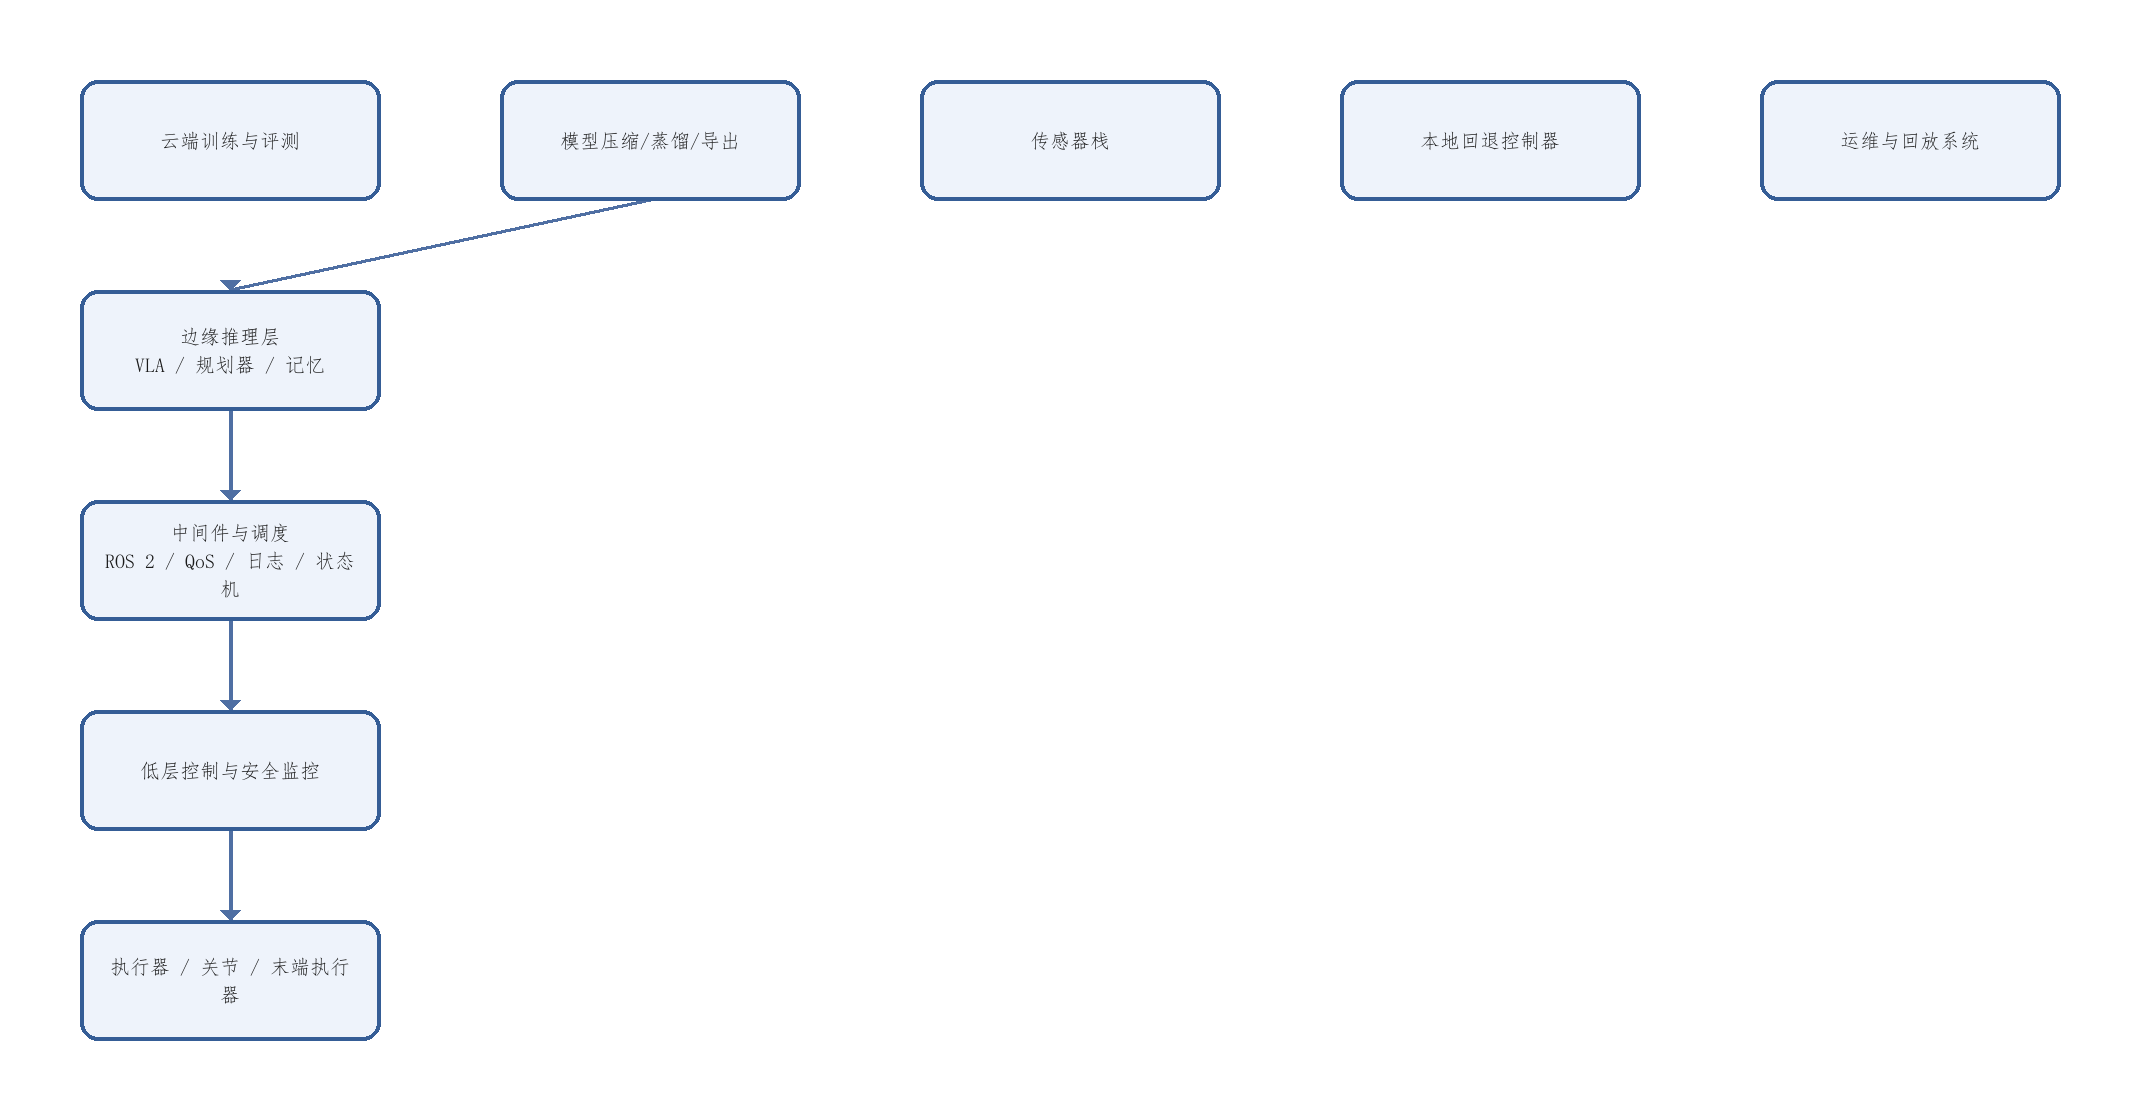
\includegraphics[width=0.9\textwidth,height=0.72\textheight,keepaspectratio]{figures/15-部署系统栈图.png}
\caption{15-部署系统栈图}
\label{fig:15-部署系统栈图}
\end{figure}

\section*{表 15-1 人形 / 固定臂 / 移动操作平台硬件约束比较表}
\addcontentsline{toc}{chapter}{表 15-1 人形 / 固定臂 / 移动操作平台硬件约束比较表}
\markboth{表 15-1 人形 / 固定臂 / 移动操作平台硬件约束比较表}{表 15-1 人形 / 固定臂 / 移动操作平台硬件约束比较表}

\begingroup
\small
\begin{xltabular}{\textwidth}{YYYYY}
\toprule
平台形态 & 主要优势 & 主要约束 & 对模型接口的影响 & 更典型的应用方向 \\
\midrule
\endfirsthead
\toprule
平台形态 & 主要优势 & 主要约束 & 对模型接口的影响 & 更典型的应用方向 \\
\midrule
\endhead
人形 & 环境兼容性强，适配人类基础设施叙事自然 & 机构复杂、能耗高、平衡与维护难度大 & 需要更强的全身协调、状态估计和安全回退 & 通用场景探索、复杂人类环境任务 \\
固定臂 & 结构稳定、控制成熟、节拍和精度可控 & 工作空间固定、环境改造依赖高 & 更适合高频稳定闭环和结构化动作接口 & 工业装配、分拣、实验室自动化 \\
移动操作平台 & 兼具导航与操作，场景灵活性更高 & 导航与操作耦合，系统栈更复杂 & 需要同时处理定位、移动安全与操作接口 & 仓储、巡检、服务机器人 \\
\bottomrule
\end{xltabular}
\endgroup

这张表的意义在于提醒读者：平台形态差异不是外形差异，而是接口预算、控制复杂度、维护成本和可商业化路径的联合变化。

% Generated from 16-安全、对齐、验证与治理.md; edit the LaTeX source after migration.

\part*{第十六部分 安全、对齐、验证与治理}
\addcontentsline{toc}{part}{第十六部分 安全、对齐、验证与治理}
\markboth{第十六部分 安全、对齐、验证与治理}{第十六部分 安全、对齐、验证与治理}

具身系统与纯软件 AI 最本质的不同之一，就是错误不再只停留在信息层，而会转化为直接的物理后果。一次错误抓取可能损坏工件，一次错误导航可能撞到人，一次错误交互可能导致危险动作被执行。因此，安全、验证与治理在机器人系统里不是最后附加的一章，而是贯穿全链路的一级问题。

随着基础模型进入机器人控制栈，这一问题进一步复杂化。传统机器人安全更强调机械风险、功能安全与工作单元隔离；大模型时代则还必须处理误解指令、错误工具调用、远程运维链路、数据治理与模型责任边界。工业机器人安全标准与 AI 风险治理框架正在逐步汇合，相关框架与标准可参见 \href{https://www.nist.gov/itl/ai-risk-management-framework}{NIST AI 风险管理框架}、\href{https://www.iso.org/standard/59820.html}{ISO 10218 机器人安全标准} 与 \href{https://www.iso.org/standard/53820.html}{ISO 13482 个人护理机器人安全标准}。

\chapter*{76. 具身安全为何是一级问题}
\addcontentsline{toc}{chapter}{76. 具身安全为何是一级问题}
\markboth{76. 具身安全为何是一级问题}{76. 具身安全为何是一级问题}

\section*{76.1 物理世界中的损害与责任}
\addcontentsline{toc}{section}{76.1 物理世界中的损害与责任}


如果把这一节再说得更具体一点，具身系统里的“损害”至少应分成四层：对人的直接伤害、对设备与工件的损害、对生产或服务流程的中断、以及事故后的责任追溯成本。这四层损害并不会等价出现，但任意一层过高，都足以改变系统是否允许上线、允许在什么速度下运行、允许由谁签字放行。因此，责任不是部署后的法律附件，而是系统设计阶段就会反向塑造动作权限和运行边界的内生变量。

也正因为如此，具身系统的很多“保守”设计并不是技术不够先进，而是责任结构的自然产物。限速、限力、工作空间裁剪、特定动作必须二次确认、异常时优先停机而非继续尝试，这些看起来降低了系统上限，却往往是把不可接受的责任暴露控制在可运营范围内的必要代价。对于学习者而言，这一点非常重要，因为它解释了为什么现实系统经常不会沿着“只要更聪明就行”的方向自然演化。 具身系统进入物理世界后，损害与责任不再只是“模型输出错了”，而是会具体落到人身伤害、设备损坏、现场停工、财产损失和责任归属争议。也正因如此，机器人安全讨论从一开始就带有更强的工程、法律和组织属性。对具身系统而言，责任不是部署后才讨论的外部问题，而是会反过来塑造权限边界、动作范围和接管策略的内部设计变量。

只要一个错误动作可能造成夹伤、跌落、流程中断或设备破坏，那么风险偏好、最大速度、接触阈值和人工接管机制就必须在架构阶段写进去。换句话说，责任不是后补文档，而是决定“哪些能力可以开放、哪些必须受限”的前置条件。 具身系统进入物理世界后，损害与责任不再只是“模型输出错了”，而是会具体落到人身伤害、设备损坏、现场停工、财产损失和责任归属争议。也正因如此，机器人安全讨论从一开始就带有更强的工程、法律和组织属性。 对具身系统而言，这种责任并不是抽象法务问题，而是直接塑造系统设计边界的工程事实。只要一个错误动作可能造成夹伤、跌落、财产破坏或流程中断，那么风险偏好、动作权限、最大速度、接触阈值和人工接管策略都必须在架构阶段被写进去。也就是说，责任不是部署后才讨论的外部问题，而是设计时就决定“哪些能力可以开放、哪些能力必须受限”的内部变量。

软件模型的错误通常造成错误信息、错误推荐或错误分类；具身系统的错误则可能造成物理伤害、财产损失和责任事故。这使得机器人安全天然比许多纯软件 AI 场景具有更高后果风险。

\section*{76.2 与纯软件 AI 风险的差异}
\addcontentsline{toc}{section}{76.2 与纯软件 AI 风险的差异}


纯软件 AI 风险与具身风险的根本差异，还体现在反馈时间尺度上。很多软件系统的错误可以通过人工复核、延迟执行、内容下架或版本回滚在事后缓解；而具身系统的错误常常在毫秒到秒级内完成并造成不可逆后果。也就是说，机器人安全更依赖前置限制、在线拦截和失效安全，而不是事后解释。

这会直接改变评价标准。一个在聊天系统里“整体准确率更高”的模型，迁移到具身闭环中时，未必比一个略保守但尾部风险更低的模型更安全。对机器人来说，灾难性偶发错误的代价常常远高于平均表现的微弱提升，因此后续所有性能讨论都应默认接受这一风险偏好差异。 与纯软件 AI 相比，机器人风险有两个额外维度。第一，错误会通过执行器直接作用于外部世界；第二，很多后果不可撤销。一个语言模型答错一句话，与一个移动平台在错误时机启动，不属于同一数量级风险。这意味着纯软件领域常用的平均性能口径，不能直接平移到具身系统。

因此，具身安全更强调尾部风险、最坏情况边界和可恢复性，而不仅仅是平均正确率。一个“整体准确率更高”但偶发灾难性错误的系统，未必比一个略保守但风险边界清楚的系统更可接受。 与纯软件 AI 相比，机器人风险有两个额外维度：第一，错误会通过执行器直接作用于外部世界；第二，很多损害不是可撤销的信息错误，而是不可逆的物理后果。这也是为什么具身系统的安全治理不能只停留在内容审核或输出过滤层面。 这类差异还意味着很多纯软件领域常见的评估口径不能直接平移过来。一个语言模型回答错一句话，和一个移动底盘在错误时间启动并不是同数量级风险；同样，传统 AI 中“平均性能更高”也未必能抵消具身系统中极低频灾难事件的不可接受性。因此，具身安全评估更强调尾部风险、最坏情况边界和可恢复性，而不仅是平均正确率。

纯软件 AI 更容易集中在信息真实性、偏见、隐私和误导风险上；具身系统则还要额外面对碰撞、跌倒、夹伤、误触发、失控移动和执行器失效等风险。

\section*{76.3 安全与商业化之间的关系}
\addcontentsline{toc}{section}{76.3 安全与商业化之间的关系}


从商业角度看，安全还会直接影响客户接受方式。客户真正购买的并不只是“机器人会做事”，而是“机器人会在多大责任边界内稳定做事”。一旦系统无法清晰回答接管规则、停机条件、事故追溯、权限分层和版本回滚，很多高价值场景即使技术上可做，也很难进入正式采购流程。换言之，安全不是在商业化之后才被补上的成本项，而是商业化成立本身的组成条件。

这也解释了为什么一些看起来更慢的路线反而更容易进入真实场景。它们也许不追求最高自治率，但更早把安全约束组织成可运营条件，因而能更快跨过客户和监管的心理门槛。对研究型报告而言，这比抽象争论“安全是否阻碍创新”更有解释力。 安全与商业化并不是天然对立，而是共同决定系统是否能进入真实运营闭环。若一个系统只有在大幅压低速度、收紧工作空间和频繁人工接管下才安全，那么它的商业价值很可能也会被显著削弱；反过来，若为了追求节拍和成本而牺牲安全边界，系统又难以获得长期部署许可。两者实际上共享同一组现实约束。

因此，更成熟的商业路线并不是“先商业化、后补安全”，而是从一开始就把安全条件写进产品定义和服务模型。谁能把安全约束组织成可运营条件，谁的商业路径才更稳。

安全与商业化之间并不是简单对立关系。短期看，更严格的安全机制确实会增加开发和部署成本；但中长期看，谁能更早把安全、验证、责任追踪和异常恢复制度化，谁反而更有机会进入高价值、高责任、高复购的真实场景。也就是说，安全不只是约束，也可能是进入更高等级市场的门票。

对具身行业尤其如此。很多场景之所以迟迟难以规模化，不是因为市场没有需求，而是因为系统尚未在安全与责任层面达到可接受阈值。因此，把安全仅仅理解为“拖慢创新”的外部负担，会低估它作为商业化前提条件的地位。 安全与商业化不是彼此独立的两条线。很多机器人产品能否真正落地，决定性因素并不是 demo 里最强能力，而是系统是否能在可接受责任边界内稳定运行。换句话说，安全不是商业化之后再补的约束，而是决定哪些场景根本可以卖、可以部署、可以长期运维的前提。

也正因为如此，很多表面上看起来“进展慢”的安全要求，实际是在帮助行业区分“可展示能力”和“可签约交付能力”。对研究报告而言，把这层关系说清楚很重要，否则很容易高估炫目 demo 的产业成熟度。

对机器人而言，安全不是阻碍商业化的额外负担，而是商业化成立的前提。没有安全保证的系统，无法进入高价值真实场景。

\chapter*{77. 安全问题分类}
\addcontentsline{toc}{chapter}{77. 安全问题分类}
\markboth{77. 安全问题分类}{77. 安全问题分类}

\section*{77.1 物理安全}
\addcontentsline{toc}{section}{77.1 物理安全}


物理安全若要真正进入系统设计，不能只停留在“不要撞人”这一口号层面，而需要明确进入动作接口。更实用的做法，是把每一类动作都绑定到可验证的速度、力、距离、接触持续时间和工作空间边界上，再通过在线监测器持续检查是否越界。这样一来，模型给出的高层意图与底层可执行安全边界之间，才真正建立起工程接口。

这一点也意味着，物理安全并不只属于控制器或机械工程师。高层策略若经常把系统推向未验证姿态、狭窄空间或高不确定接触区，底层再稳也会不断被动兜底。因此，物理安全是典型的跨层问题，必须贯穿高层任务规划、中层技能调用与底层控制闭环。 物理安全关注的是“机器人动作本身会不会直接伤人、伤设备、伤环境”。它通常涉及速度、力、碰撞能量、可达区域、急停机制、隔离边界和人机接触条件。与纯软件系统不同，这里的错误不是输出错一句话，而可能是夹伤、撞击、跌落或设备损坏。

一个最小物理安全约束可以抽象为：

\begin{equation*}
a_t \in \mathcal{A}_{safe}(x_t, e_t)
\end{equation*}

其中 \(\mathcal{A}_{safe}\) 表示在当前机器人状态 \(x_t\) 与环境状态 \(e_t\) 下允许执行的安全动作集合。 物理安全看似最传统，但在基础模型进入机器人后反而更需要重新审视。原因在于，高层策略的开放性增强后，机器人更可能进入过去没有显式编排过的姿态、路径和交互模式，从而触发底层原本不常见的碰撞或过载风险。因此，物理安全不只是底层控制器的事情，也取决于高层是否把系统推进了未经充分验证的状态区域。

涉及碰撞、力过载、稳定性失控、危险接触和环境破坏。

\section*{77.2 功能安全}
\addcontentsline{toc}{section}{77.2 功能安全}


功能安全的核心，不在于“平时性能高不高”，而在于“出现异常时系统是否还能退回到定义清楚的安全模式”。这一点对具身系统极其关键，因为很多危险并不是来自模型胡来，而是来自传感器掉线、节点卡死、时钟不同步、控制回路超时、执行器失配或软件版本不兼容。系统若没有明确的降级逻辑，就会在这些局部异常下以不可预测方式继续动作。

因此，一个成熟的功能安全设计通常需要显式定义状态机：正常运行、受限运行、等待确认、人工接管、安全停机、故障锁定等状态如何切换，触发条件是什么，谁有权恢复。只有这些内容被写成系统行为的一部分，功能安全才不是口头承诺。 功能安全更关心“系统在部件失效、输入异常或状态不一致时，是否仍能进入可控状态”。它不只讨论机器人平时做得对不对，而更关注传感器丢失、节点重启、通信中断、控制器卡死时，系统是否会失控或是否能够优雅降级。

一个极简功能安全思路可以写成：

\begin{lstlisting}[language=python]
if sensor_fault or controller_timeout:
    enter_safe_mode()
    notify_operator()
\end{lstlisting}

功能安全更关心“系统在部件失效、输入异常或状态不一致时，是否仍能进入可控状态”。它不只讨论机器人平时做得对不对，而更关注传感器丢失、节点重启、通信中断、控制器卡死时，系统是否会失控或是否能够优雅降级。

对学习者来说，可以把它理解为：物理安全更像“不要撞”，功能安全更像“出了错也不要以不可控方式撞”。

涉及故障检测、异常停机、冗余设计、控制回退和失效安全机制。很多风险不来自“模型胡来”，而来自系统在局部异常下没有及时进入安全模式。

\section*{77.3 网络与数据安全}
\addcontentsline{toc}{section}{77.3 网络与数据安全}


网络与数据安全在具身系统里还有一个经常被低估的特点：攻击不一定要直接命中控制接口，也可能通过污染感知流、篡改任务配置、劫持更新链路、注入伪造日志或窃取环境布局数据间接造成严重后果。这意味着机器人系统的攻击面往往比看上去更宽，因为任何能影响观测、策略、更新或接管流程的入口，都可能变成行动风险入口。

所以更合理的安全设计，不是简单把机器人接上企业网络，而是按最小权限原则重新切分数据面、控制面和运维面。谁能看、谁能写、谁能下发任务、谁能更新版本、谁能远程接管，都应有明确分层。这种分层看似“IT 化”，实际是具身系统运行安全的组成部分。 网络与数据安全在机器人里尤其敏感，因为很多系统会同时暴露远程控制接口、现场视频流、内部地图、任务日志和设备身份信息。一旦这些链路被入侵，不只是数据泄露，还可能直接引发错误动作、远程操控或安全停机失效。对于联网机器人来说，这已经不是传统 IT 附属议题，而是运行安全的一部分。

更进一步看，远程更新、云端推理、遥操作接管和日志回传都在扩大攻击面。攻击者甚至未必需要直接控制执行器，只要能污染感知输入、篡改任务配置或劫持更新链路，就可能制造严重事故。因此，网络与数据安全必须进入具身系统的主架构讨论，而不能留在部署末端补救。 网络与数据安全在机器人里尤其敏感，因为很多系统会同时暴露远程控制接口、现场视频流、内部地图、任务日志和设备身份信息。一旦这些链路被入侵，不只是数据泄露，还可能直接引发错误动作、远程操纵或安全停机失效。 对于联网机器人，这一类风险的重要性正在快速上升。远程更新、云端推理、遥操作接管、日志回传和多设备协同都在扩展攻击面。攻击者未必需要直接控制执行器，只要能够污染感知输入、篡改任务配置、劫持更新链路或读取高价值环境数据，就可能造成安全事故或隐私事件。因此，网络与数据安全在具身系统中不应被视为 IT 附属议题，而是运行安全的一部分。

机器人越来越联网、越来越依赖远程更新和云端协同，这意味着攻击面也显著扩大。感知数据、控制接口和远程运维链路都可能成为安全漏洞。

\section*{77.4 模型行为安全}
\addcontentsline{toc}{section}{77.4 模型行为安全}


模型行为安全最棘手的地方，在于它往往发生在系统“看起来还在正常工作”的时候。模型可能没有明显崩溃，也没有输出完全荒谬的动作，但它可能误解禁止条件、跳过关键前置步骤、对异常状态过度自信，或在模糊指令下选择不安全默认动作。相比底层控制失稳，这类错误更难被第一时间察觉，因为它们首先表现为“决策合理性”失真，而不是“机械系统明显坏掉”。

因此，模型行为安全更像决策权限管理问题，而不是单纯“让模型更聪明”问题。一个更适合工程实现的抽象是：

\begingroup
\footnotesize
\begin{equation*}
a_t = \Pi_{\text{safe}}\!\left(\pi_\theta(h_t), x_t\right)
\end{equation*}
\endgroup

其中 \(\pi_\theta\) 负责给出高层动作建议，\(\Pi_{\text{safe}}\) 负责把动作投影回安全可行集，\(x_t\) 则包含本体状态、工作空间约束、权限边界与监视器信号。若系统里根本没有 \(\Pi_{\text{safe}}\) 这一层，那么再高分的基础模型也只是把高风险决策直接暴露给执行器。

从风险形态看，模型行为安全至少包括四类问题：

\begin{enumerate}
\item 语义失配：把“拿起蓝杯”错听成“移动左侧全部物体”。
\item 阶段失配：没有先建立约束或接触条件，就直接进入执行阶段。
\item 恢复失配：系统已经偏航，却把“继续尝试”误当成安全恢复。
\item 置信失配：对分布外输入仍高置信输出具体动作。
\end{enumerate}

因此，行为安全必须依赖多层机制，而不能只靠训练时对齐。动作裁剪、工作空间约束、接触阈值监测、技能白名单、任务级回退逻辑和人在回路审批，往往需要与模型本体共同组成联合安全系统。对高责任场景而言，最危险的从来不是“模型完全不会”，而是“模型多数时候看起来会，因此偶发越界更难被人类及时察觉”。

\chapter*{78. 验证与测试框架}
\addcontentsline{toc}{chapter}{78. 验证与测试框架}
\markboth{78. 验证与测试框架}{78. 验证与测试框架}

\section*{78.1 仿真验证}
\addcontentsline{toc}{section}{78.1 仿真验证}


仿真验证最常见的误区，是把它理解成“只要仿真里跑通，就算安全被验证了”。更准确的理解应该是：仿真主要负责以更低成本扩大覆盖范围，帮助团队系统性穷举边界条件、稀有工况和危险组合，而不是代替真实世界认证。它擅长发现明显问题、构造危险场景和形成大规模回归集，却无法自动保证接触细节、传感器噪声和现场组织行为与现实完全一致。

因此，一个更成熟的仿真验证策略通常不是追求“仿真等于现实”，而是明确划分三件事：仿真负责发现什么，真机负责确认什么，事故回放负责追什么。只有这三者被协同组织起来，仿真验证才真正成为安全基础设施，而不是论文附图。

一个最小验证流程通常是：

\begin{lstlisting}[language=python]
for scenario in adversarial_or_random_scenarios:
    result = run_policy_in_sim(policy, scenario)
    log_safety_metrics(result)
\end{lstlisting}

仿真验证最有价值的地方，不只是“省成本”，而是它能系统性覆盖现实里不便频繁制造的危险条件，例如极端障碍布局、罕见接触失稳、执行器迟滞放大、传感器失配和异常人类介入。对安全工程来说，仿真更像风险放大镜，帮助团队在真实上线前主动寻找脆弱点，而不是只验证系统在理想流程中是否能通关。

从证据结构看，仿真验证至少应该沉淀三类资产：场景模板、扰动模板和失效判据。前两者决定“你是否系统性地找边界”，后者决定“系统究竟是在什么条件下被判失败”。没有这三类资产，仿真结果再多也很难变成可重复利用的安全证据。

\section*{78.2 真机验证}
\addcontentsline{toc}{section}{78.2 真机验证}


真机验证的独特价值，在于它能揭示所有“只有放到真实硬件和真实现场才会出现”的耦合问题。包括轻微机械偏差、夹爪磨损、热漂移、地面摩擦差异、传感器脏污、通信抖动、操作员习惯和现场临时变化，这些问题往往不会完整出现在仿真中，却会在长期运行中不断积累成事故风险。

因此，真机验证不应只追求“再做几次成功 demo”，而应刻意组织重复、疲劳、扰动和恢复测试。真正高价值的真机验证，不是证明系统可以成功一次，而是识别它在第十次、第一百次、不同班次和不同轻微偏差下是否还能保持受控。

更严谨的做法，是把真机验证组织成分阶段放行：

\begin{enumerate}
\item 台架/空载阶段：检查急停、限速、关节限位、接管链路。
\item 封闭工位阶段：检查代表性任务、低风险异常和恢复策略。
\item 影子运行阶段：真实流程旁路观察，不直接控制最终结果。
\item 扩容阶段：在限定权限下逐步扩大场景与班次覆盖。
\end{enumerate}

这样真机验证才是系统工程，而不只是展示环节。它的目标，是确认那些在仿真与离线分析中看起来成立的安全机制，在真实传感器、真实时延和真实机械误差下是否仍然成立。它通常规模更小、成本更高，但证据强度也更高，因为很多关键风险只会在真实本体上暴露出来。

一个极简真机验证流程可以写成：

\begin{enumerate}
\item 选定受控场景和风险边界。
\item 逐项测试急停、限速、接管、异常恢复。
\item 记录碰撞、误停、迟滞和误报情况。
\item 审核是否满足继续扩大测试范围的条件。
\end{enumerate}

真机验证更接近真实风险，因此对安全论证至关重要。但它昂贵、慢，且本身也可能带来测试风险，所以必须和仿真回归、事故回放、版本审计一起形成闭环。

\section*{78.3 红队测试与异常工况测试}
\addcontentsline{toc}{section}{78.3 红队测试与异常工况测试}


红队测试最有价值的地方，不只是找 bug，而是建立一张“系统在何种组合条件下失去可控性”的风险地图。对具身系统来说，真正危险的场景往往不是单一异常，而是多种轻微异常叠加，例如模糊指令叠加遮挡、网络延迟叠加执行器失准、物体替换叠加接触滑移。正常测试流程很难系统覆盖这些组合，而红队测试恰恰应以构造这些组合为目标。

这意味着红队结果不应只留下一个失败清单，更应沉淀成可复测资产：危险场景模板、异常输入集、回放脚本、接管记录与版本回归集。只有这样，红队测试才会从一次性审查动作变成持续的安全生产力。

一个更成熟的异常工况库通常至少包括四类扰动：

\begin{enumerate}
\item 语义扰动：模糊指令、冲突指令、越权请求。
\item 感知扰动：遮挡、反光、错检、标定偏移、时间不同步。
\item 执行扰动：迟滞、掉帧、轻微失准、抓取对象替换。
\item 组织扰动：人类临时介入、工位改造、网络抖动、远程接管延迟。
\end{enumerate}

异常工况测试的价值，还在于把低频问题显式纳入版本回归。若每次系统升级只看平均成功率，而不复测历史上最危险的异常案例，那么能力提升很可能伴随风险回归。真正成熟的验证体系，应把这些异常样本当作核心资产。

近年一个很有启发性的变化，是安全 benchmark 开始不再只看“任务做成没有”，而把治理、恢复与升级安全一起拉进评测范围。\href{https://arxiv.org/abs/2604.11174}{EmbodiedGovBench：具身系统治理、恢复与升级安全基准} 就明确把具身智能体的治理、恢复与升级安全作为独立维度来评估。这一点非常重要，因为它意味着红队测试的目标不再只是证明“模型会不会出错”，而是要回答：出错后能否被及时发现，发现后能否进入正确恢复链路，版本升级后这些老问题会不会重新回来。

若把红队资产化写成最小闭环，它更像下面这条流程：

\begin{lstlisting}[language=python]
for scenario in red_team_library:
    outcome = run_system(build_stress_case(scenario))
    log(outcome, scenario.tags, current_version)
    if outcome.is_catastrophic or outcome.recovery_failed:
        add_to_regression_suite(scenario)
        tighten_release_gate(current_version, scenario)
\end{lstlisting}

这段伪代码的重点不在实现细节，而在于强调：真正成熟的红队测试不是“一次性把系统弄崩”，而是把失败样本自动转成回归资产和版本放行约束。也就是说，红队测试必须同时服务发现、追责和长期治理三件事，否则它只会停留在安全审查表演层。

\section*{78.4 人在回路与人工接管机制}
\addcontentsline{toc}{section}{78.4 人在回路与人工接管机制}


人在回路的成熟度，关键不在“有没有人工接管”，而在“接管是否设计成了一套稳定接口”。这包括接管条件是否明确、操作员能否快速理解当前上下文、接管后系统是否会进入一致状态，以及接管记录是否能回流到后续训练和验证链路。若这些内容没有设计清楚，人工接管就会变成临时补丁，而不是正式安全机制。

一个成熟的接管设计通常会把人工角色拆成至少三层：

\begin{enumerate}
\item 批准层：确认高风险动作是否被允许执行。
\item 监督层：观察系统退化，必要时要求降级或暂停。
\item 执行层：在系统已经越界或失效时直接接管。
\end{enumerate}

这样做的意义，不是让人类替机器人做完所有事，而是把最稀缺的人类判断留给最关键节点。从产品形态看，共享自治之所以经常是现实最优解，并不是因为企业放弃了自治，而是因为它把“高价值判断”与“高频执行”做了更稳妥的分工。

若把系统风险写成条件风险函数，则可以抽象记为：

\begingroup
\scriptsize
\begin{equation*}
\mathcal{R} = \mathbb{E}_{x \sim p(x)}[\text{loss}(x)] + \lambda \, \mathbb{P}(\text{catastrophic event})
\end{equation*}
\endgroup

这里第一项对应一般性能退化，第二项对应灾难性事件风险。对具身系统而言，后一项的权重 \(\lambda\) 往往远高于纯软件任务。

但“人在回路”并不等于“任何时候都让人接管”。更准确的工程问题是：\texttt{\detokenize{在哪些节点要求人类批准，哪些节点要求人类监督，哪些节点允许人类直接覆写动作}}。若把人类权限强度记为 \(\alpha_t \in [0,1]\)，可以把最简单的共享自治写成

\begingroup
\footnotesize
\begin{equation*}
a_t = \alpha_t a_t^{\text{human}} + (1-\alpha_t) a_t^{\text{auto}}
\end{equation*}
\endgroup

不过这只是最粗糙的形式。真实系统中更重要的不是连续混合动作本身，而是 \(\alpha_t\) 何时变化、由谁变化、变化依据什么证据。否则系统就会出现一种很危险的假象：表面上“有人在回路”，实际上人类既没有足够上下文，也没有清晰权限边界，只是在最后时刻被动兜底。

这也是为什么近年的共享自治研究越来越强调层级分工与接管接口设计，而不只强调“让人能插手”。\href{https://arxiv.org/abs/2307.01943}{面向关节型机器人的层级规划与策略塑形共享自治} 更接近一种高层任务规划与低层形状约束共同作用的写法；而相邻领域的 \href{https://arxiv.org/abs/2505.09889}{Diffusion-SAFE：安全的人机驾驶接管扩散框架} 则提醒我们，简单动作拼接或朴素交接本身也可能带来新的不安全瞬间。把这些启发迁移到具身系统里，一个更稳健的接管原则是：高层批准、中层监督、低层急停三种权限应当被显式区分，而不是统一丢给“人工可接管”这一句模糊承诺。

\section*{78.5 从“测试很多次”到“证据链足够”的跃迁}
\addcontentsline{toc}{section}{78.5 从“测试很多次”到“证据链足够”的跃迁}


具身系统最容易出现的一种幻觉，是把“已经测了很多次”误当成“已经有足够证据可部署”。前者是样本数量概念，后者是证据结构概念。真正可用于放行的证据，至少要覆盖四类问题：系统在正常工况下是否稳定，系统在边界工况下如何退化，系统在异常工况下如何进入安全状态，以及版本更新后历史风险是否会重新出现。若这四类问题没有被分别回答，那么测试次数再多，也仍可能只是重复验证容易成功的主路径。

更工程化地看，安全证据链可以被抽象成一个矩阵：纵轴是工况类型，横轴是系统层级。工况类型至少包括正常、边界、异常和恢复后复测；系统层级至少包括硬件、控制、感知、模型、任务编排和运维接口。所谓“闭环”，本质上就是要求团队不要只在矩阵的某一行或某一列堆证据，而要覆盖那些最可能在跨层耦合处失真的区域。

若用一个粗略记号来表达证据覆盖度，可写成：

\begingroup
\scriptsize
\begin{equation*}
\text{Coverage} = \sum_{c \in \mathcal{C}} \sum_{l \in \mathcal{L}} w_{c,l} \cdot \mathbf{1}[\text{tested}(c,l)]
\end{equation*}
\endgroup

其中 \(\mathcal{C}\) 表示工况集合，\(\mathcal{L}\) 表示系统层级集合，\(w_{c,l}\) 表示不同组合的重要性权重。它不是审计公式本身，但足以提醒我们：安全验证的关键不只是“做了多少测试”，而是“关键组合有没有被碰到”。

若把版本放行再写得更明确，可近似表达为：

\begingroup
\scriptsize
\begin{equation*}
\text{Gate}(v)=\mathbf{1}\!\left[
C_{\text{normal}}\!\ge\!\tau_1 \land
C_{\text{edge}}\!\ge\!\tau_2 \land
C_{\text{recovery}}\!\ge\!\tau_3 \land
C_{\text{regression}}\!\ge\!\tau_4
\right]
\end{equation*}
\endgroup

其中 \(C_{\text{normal}}\)、\(C_{\text{edge}}\)、\(C_{\text{recovery}}\)、\(C_{\text{regression}}\) 分别表示正常工况、边界工况、异常恢复和历史风险回归的证据覆盖度。真正成熟的放行口径不应是“主流程成功率上升了”，而应是“关键风险组合的未解释空白在收缩”。

\chapter*{79. 标准、认证与治理}
\addcontentsline{toc}{chapter}{79. 标准、认证与治理}
\markboth{79. 标准、认证与治理}{79. 标准、认证与治理}

\section*{79.1 机器人安全标准}
\addcontentsline{toc}{section}{79.1 机器人安全标准}


安全标准的真正作用，不只是给出一张合规检查表，而是提供一种跨组织可共享的安全语言。它帮助供应商、客户、集成商、认证方和监管方在同一套术语下讨论风险来源、测试范围、责任分工和验收条件。没有这种公共语言，再强的技术能力也很难转化成可规模化采购的产品能力。

因此，本节最值得读者把握的不是标准编号本身，而是标准如何反向要求系统留下证据链：哪些风险被识别了、哪些约束被实施了、哪些工况被测试了、哪些异常会触发停机、哪些版本更新需要重新认证。这些要求会直接改变系统工程方式。

工业机器人、协作机器人与服务机器人各自有不同标准框架，\href{https://www.iso.org/standard/59820.html}{ISO 10218} 与 \href{https://www.iso.org/standard/53820.html}{ISO 13482} 仍是理解产业安全边界的两个基础入口。更值得注意的是，2026 年一篇对 ISO 10218:2011 与 ISO 10218:2025 的比较分析，把新增重点概括为功能安全与网络安全要求的增强，这说明标准口径正在从“机械本体防护”继续扩展到“联网系统与软件行为”层，参见 \href{https://arxiv.org/abs/2602.17822}{《工业机器人安全要求演进比较分析》}。

因此，标准不是技术之外的文书负担，而是工程系统的上游约束。谁忽视这一点，谁就会在从实验室走向现实部署时突然发现整条验证链都需要重建。

\section*{79.2 AI 治理与责任边界}
\addcontentsline{toc}{section}{79.2 AI 治理与责任边界}


责任边界之所以在大模型进入具身系统后变得更复杂，是因为最终行为往往由多方共同塑造：底座模型提供先验，系统集成商定义接口，场景运营方决定流程和权限，客户又拥有最终使用环境。这样一来，很多事故不再能简单归因于某一段代码或某一台硬件，而是必须放回整条权责链上理解。

因此，治理问题的重点不只是追责，更是预先设计谁能审计什么、谁能修改什么、谁有暂停权限、谁负责事故复盘、谁触发重新验证。权责链若设计得模糊，技术系统越复杂，部署风险反而越高。

一个更实用的治理视角，是把责任边界固定到四类问题上：

\begin{enumerate}
\item 谁声明能力边界。
\item 谁批准风险接受水平。
\item 谁持有运行期日志与接管权限。
\item 谁在更新后负有再验证义务。
\end{enumerate}

这与近年的 AI 风险管理研究是一致的：可审计性、可追踪性和版本化责任分工，不是附属治理层，而是高风险 AI 系统的工程前提，参见 \href{https://arxiv.org/abs/2401.15229}{《AI 风险管理的演化》}。对行业跟踪来说，这一节最重要的观察口径是：谁在主动建设可审计链路，谁就在为大规模部署铺路。

如果把治理写得更接近当前行业语言，NIST 的表述其实很值得借用。\href{https://www.nist.gov/itl/ai-risk-management-framework}{NIST AI Risk Management Framework 官方页面} 明确把 AI RMF 定义为一套可自愿采用的风险管理资源，用于把“可信性考量”纳入设计、开发、使用和评估。对具身系统来说，这一点尤其关键，因为机器人风险本就跨越设计、训练、部署和运维多个阶段。也就是说，治理不应被理解成上线之后的外部审查，而应被理解成全生命周期中的一套风险分配机制。

因此，责任边界最好不要只写成“谁背锅”，而应写成一张持续运行矩阵。一个更可执行的四角色视图是：

\begin{enumerate}
\item 能力声明者：声明模型、本体和技能的已验证边界。
\item 部署批准者：决定哪些边界在当前客户或场景下可被接受。
\item 现场运营者：持有日志、接管、暂停和灰度放量权限。
\item 事故复盘者：在事后界定问题属于能力缺陷、流程缺陷还是边界设定错误。
\end{enumerate}

只要这四个角色中的任一角色含糊不清，治理就会迅速退化成“系统很复杂，所以谁都说不清”。而具身系统恰恰最怕这种模糊，因为责任模糊会直接放大部署风险。

\section*{79.3 数据与场景合规}
\addcontentsline{toc}{section}{79.3 数据与场景合规}


数据与场景合规在具身系统中比纯内容系统更复杂，因为机器人采到的不只是“数据内容”，而是常常连同空间布局、操作流程、人员活动、设备配置和组织节奏一起被记录和回放。这意味着很多数据即使不包含明显敏感文本，也可能仍然包含高价值、高敏感的现场知识。

因此，合规问题不能被压缩成一条数据免责声明。它应被写进采集流程、数据分级、访问权限、场景准入和后续训练复用规则中。更准确地说，具身系统的合规对象至少有两层：一层是数据对象，另一层是场景对象。前者回答“能不能存、能不能训、能不能共享”，后者回答“机器人能不能进入这里、能不能在这里持续回放与学习”。如果只做第一层而忽略第二层，现场合规风险仍然会不断泄漏。

若再往下拆，数据与场景合规至少应被写成四层。第一层是\texttt{\detokenize{数据权属层}}，关注视频、音频、日志、工艺参数和标注是否有采集与训练授权；第二层是\texttt{\detokenize{空间隐私层}}，关注环境布局、人员活动轨迹和设备配置是否属于敏感现场知识；第三层是\texttt{\detokenize{流程合规层}}，关注机器人是否被允许进入某类工位、时间段和操作环节；第四层是\texttt{\detokenize{运维日志层}}，关注远程诊断、事故回放和模型更新记录是否满足最小必要与可追溯原则。只要其中任一层缺失，系统就可能在“技术上可行、治理上失格”的状态下被错误推进。

对长期维护报告而言，这一节还有一个很实际的含义：以后凡出现“某公司拥有大量真实场景数据”这种判断，都应同时追问这些数据的授权结构、场景使用边界和回放权限。否则，“数据优势”很容易被误写成无条件正向信号，而忽略其同时伴随的合规成本和潜在部署约束。

\section*{79.4 安全基础设施的新趋势}
\addcontentsline{toc}{section}{79.4 安全基础设施的新趋势}


一个越来越清楚的趋势是，安全正在从“单点算法能力”转向“平台化工程能力”。真正有长期价值的，不再只是某个碰撞检测器或某个风险分类器，而是围绕版本审计、影子测试、异常回放、权限分层、远程停机、灰度发布和事故复盘建立起来的一整套持续运行体系。谁能把这些机制做成默认基础设施，谁就更接近大规模部署门槛。

这也是本章与后文企业、商业化和政策章节的接口所在。后续评估一家公司或一条路线时，不应只问“有没有安全模块”，而应问“有没有安全基础设施”。前者只是组件，后者才是组织化能力：能否在模型更新后自动回归、能否在事故后快速复盘、能否在多现场部署中保持统一权限与日志口径。

从运行栈角度看，安全基础设施至少应覆盖七个动作：版本追踪、影子运行、异常回放、灰度放量、远程停机、权限审计和事故归档。任何一项长期缺位，最后都会以某种“系统明明变强了却更难运营”的形式反噬部署节奏。

下面给出一个极简安全监控伪代码，用于说明部署阶段的分层拦截思路：

\begin{lstlisting}[language=python]
action = policy(observation, goal)

if not safety_filter.within_limits(action, robot_state):
    action = safety_filter.project_to_safe_set(action)

if anomaly_detector.triggered(robot_state, observation):
    supervisor.request_handover()
    action = emergency_controller.stop()
\end{lstlisting}

\section*{79.5 一个更可执行的治理操作模型}
\addcontentsline{toc}{section}{79.5 一个更可执行的治理操作模型}


如果把“治理”从抽象原则翻译成日常运转机制，一个更可执行的做法是明确四个固定角色：能力提供者、部署批准者、现场运营者与事故复盘者。能力提供者负责声明模型、技能和本体的已验证边界；部署批准者负责决定哪些边界在当前场景下被接受；现场运营者负责运行中监控、接管与日志留存；事故复盘者则负责在事后判断问题属于能力缺陷、流程缺陷还是边界设置失误。

这种分工之所以重要，是因为很多具身事故并不是“谁犯了单一错误”，而是“多个角色都以为某件事由别人负责”。例如模型方认为某种长尾情形应由系统层兜底，系统层认为该动作在现场根本不该开放，现场方又误以为既然演示过就意味着已被默认放行。只要权责没有被结构化写清，安全问题就会在组织边界上反复泄漏。

因此，本章对治理的最强主张并不是“增加更多文书”，而是把部署前、运行中、事故后这三类决策都绑定到明确责任人上。谁批准过边界，谁保存了什么证据，谁有权暂停，谁负责重新验证，这些内容一旦清楚，很多看似复杂的治理问题就会转化为可管理的工程接口问题。

若把这一模型再落成更可执行的运行面板，一个最低可用治理面板至少应持续记录四类指标：

\begin{enumerate}
\item \texttt{\detokenize{边界指标}}：当前版本允许哪些动作、在哪些工位、以什么速度和权限运行。
\item \texttt{\detokenize{接管指标}}：接管触发频率、接管延迟、接管后是否进入一致状态。
\item \texttt{\detokenize{回归指标}}：历史危险样本是否在新版本中重新出现，是否新增未解释空白。
\item \texttt{\detokenize{审计指标}}：日志是否完整、责任链是否可追溯、版本放行是否有明确签字与依据。
\end{enumerate}

这类面板的重要性，在于它把“治理”从抽象责任讨论，压回可持续维护的数据结构。类似 \href{https://arxiv.org/abs/2604.11174}{EmbodiedGovBench：具身系统治理、恢复与升级安全基准} 这类工作真正提供的启发，也不是某一个具体分数，而是把恢复、治理与升级安全当成可以持续评测的对象。对具身系统而言，只要这些指标长期缺位，所谓治理就很容易退化成“事故之后再开会解释”；只有它们被前置写入日常运转面板，治理才会真正成为系统能力的一部分。

\section*{79.6 版本更新后的再验证门槛}
\addcontentsline{toc}{section}{79.6 版本更新后的再验证门槛}


大模型进入机器人系统之后，一个极易被低估的风险是“轻微更新也可能改变整体行为边界”。纯控制系统中，很多修改可以通过局部分析判断影响范围；但在带有基础模型、策略蒸馏、检索记忆或任务编排器的系统里，一次看似不大的模型更新、提示模板更新、工具调用顺序调整，甚至都可能让系统在旧场景里表现得像一个新系统。因此，再验证不应只在“大版本升级”时启动，而应围绕“行为边界是否可能改变”来触发。

一个更实用的再验证分类方法，是先问这次更新属于哪一层：

\begin{enumerate}
\item 参数层更新：仅改权重或阈值，但不改接口。
\item 接口层更新：改变感知输入、动作输出、工具调用或权限分层。
\item 场景层更新：进入新的客户流程、新的工位或新的运维链路。
\item 治理层更新：改变接管权限、日志留存、放行规则或回滚策略。
\end{enumerate}

只要更新触及后面三层中的任一层，就不应把它视为纯粹的低风险维护更新，而应触发历史异常样本回归、关键场景复测与放行记录更新。对研究与产业跟踪而言，这一节的含义非常直接：谁已经形成了“更新即回归、回归即审计”的机制，谁才更接近真正可运营的基础模型机器人体系。

本部分的结论是：具身系统的安全不应被理解为“控制器够稳就行”，而是一整套从高层行为边界到底层失效安全、从仿真测试到真机验证、从模型责任到部署治理的系统工程问题。也因此，本章最适合充当全书的“否决层”：很多路线在模型能力、数据规模和商业故事上都可能越来越强，但只要其接管边界、日志可追溯性、异常回退、红队覆盖和版本回滚能力没有同步成熟，就不应轻易上修整体判断。

\chapter*{图 16-1 安全、验证与治理闭环图}
\addcontentsline{toc}{chapter}{图 16-1 安全、验证与治理闭环图}
\markboth{图 16-1 安全、验证与治理闭环图}{图 16-1 安全、验证与治理闭环图}

\noindent\textit{源文件：\texttt{\detokenize{assets/diagrams/16-安全验证治理闭环图.mmd}}}

\begin{figure}[htbp]
\centering
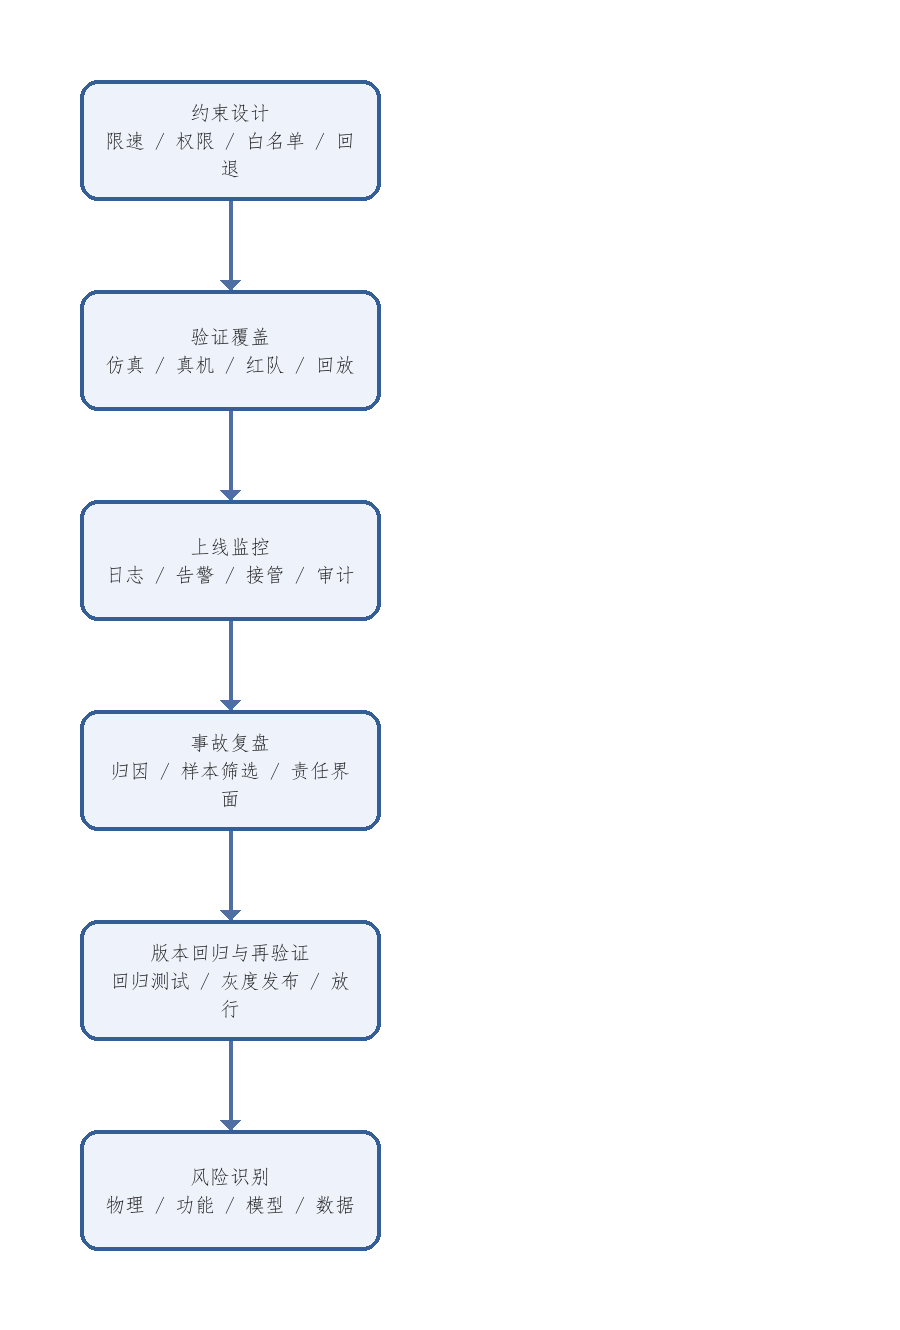
\includegraphics[width=0.9\textwidth,height=0.72\textheight,keepaspectratio]{figures/16-安全验证治理闭环图.png}
\caption{16-安全验证治理闭环图}
\label{fig:16-安全验证治理闭环图}
\end{figure}

\chapter*{图表与验证补充}
\addcontentsline{toc}{chapter}{图表与验证补充}
\markboth{图表与验证补充}{图表与验证补充}

进一步说，本章最应该服务于后文的地方，是把“安全成熟度”从抽象口号改写成可检查的结构。以后无论评估企业、产品还是论文，只要能够沿着“风险识别、约束设计、验证覆盖、上线监控、事故恢复”五步链条去问问题，就能避免把安全理解成单一合规模块。 本章后续最应被固定为正式内容的，是“物理安全 / 功能安全 / 模型安全 / 数据安全”的分类图，以及“仿真验证 - 真机验证 - 红队测试 - 现场监控”的验证闭环图。前者用于防止安全讨论沦为泛泛而谈，后者则强调安全不是单次测试，而是贯穿模型生命周期的持续验证过程。

对全书而言，这两张图也承担公共框架作用，因为它们会在企业分析、商业化、政策与部署章节中被反复引用。

\texttt{\detokenize{图 16-1 安全、验证与治理闭环图}} 的关键作用，是把“风险类型分层”与“验证运营流程分层”放到同一闭环里统一观察。这样读者就不会把安全只理解成事故清单，也不会把验证只理解成上线前测试，而能看到风险识别、验证执行、版本回归、现场监测与治理反馈之间的连续关系。对具身系统而言，这种闭环视角比单独罗列安全术语更接近真实部署逻辑。

% Generated from 17-学术前沿技术专题.md; edit the LaTeX source after migration.

\reportpart{第十七部分 学术前沿技术专题}
\addcontentsline{toc}{part}{第十七部分 学术前沿技术专题}
\markboth{第十七部分 学术前沿技术专题}{第十七部分 学术前沿技术专题}

前面的章节已经建立了主干结构，本部分则集中讨论当前最值得跟踪的一批前沿问题。这些问题未必都已形成稳定产业路径，但它们最能暴露现代具身系统的真实能力边界，也最有可能在未来几年牵引模型、数据和本体设计的进一步分化。

本章的写法刻意不追求“热点罗列”，而更强调这些前沿方向各自卡在哪些瓶颈、为什么难、以及它们会反向推动哪些基础技术继续演化。很多真正有价值的前沿，不是因为它们最会讲故事，而是因为它们迫使研究者同时面对感知、接触、推理、控制和评测的多重困难。

\section*{80. 通用操作与灵巧操作}
\addcontentsline{toc}{chapter}{80. 通用操作与灵巧操作}
\markboth{80. 通用操作与灵巧操作}{80. 通用操作与灵巧操作}

\subsection*{80.1 通用抓取}
\addcontentsline{toc}{section}{80.1 通用抓取}


通用抓取之所以依旧是前沿专题，是因为它看起来像“基础能力”，实际上却牵动感知、几何、接触、控制与恢复的多层协同。系统若只能在已知物体、已知摆放和已知夹具条件下抓取，它解决的仍然是局部模板问题；只有当它能在对象变化、姿态变化和局部遮挡下保持稳定，抓取能力才开始接近更通用的操作入口。

因此，通用抓取不是一个已经做完的老问题，而是后续很多 VLA、触觉与世界模型路线是否真正落地的最低压测场之一。 通用抓取之所以长期是前沿主题，不是因为“抓东西”本身新，而是因为它要求系统在对象类别、材质、摆放方式、遮挡关系和接近路径都变化时，仍能形成稳定抓取。它同时考验感知、几何推理、接触控制和失败恢复，因此常被当作具身系统最基础也最顽固的能力基准之一。

通用抓取看起来是最基础的问题，但它至今仍是具身系统的重要瓶颈，因为对象多样性、遮挡、摩擦变化和接触不确定性始终存在。即便在基础模型时代，“看懂物体”也不等于“找到可执行抓取方式”。

通用抓取之所以仍然是前沿问题，并不是因为学界还没学会“把东西拿起来”，而是因为一旦对象库扩大、遮挡增加、材料变化、接触条件变化或任务上下文不同，抓取就会迅速从几何问题变成感知、接触和恢复共同参与的问题。也就是说，抓取是最基础的任务单元之一，但恰恰因为基础，几乎所有系统性短板都会在这里暴露。 这也是为什么通用抓取长期具有指标意义：谁能稳定提升抓取在长尾物体、复杂遮挡和失败恢复下的表现，谁就更可能真正改善具身系统的通用性，而不是只在少数干净场景里演示漂亮结果。

\subsection*{80.2 精细装配}
\addcontentsline{toc}{section}{80.2 精细装配}


精细装配之所以特殊，是因为它把误差容忍度压得极低。相比抓取和搬运，装配往往更依赖局部几何对准、接触过程感知、高频闭环修正和阶段性失败恢复。很多系统在非接触任务中看似稳定，一进入装配就会暴露出观察误差、控制滞后与接触建模不足。

因此，精细装配在研究中始终具有标杆意义。它不是为了展示炫技，而是在迫使系统回答“当误差预算极小、接触过程主导成败时，智能究竟如何组织”。 精细装配比通用抓取更进一步，因为它要求机器人在极小几何公差、复杂接触序列和高失败代价下稳定完成任务。这里的问题不只是“把对象抓起来”，而是“在接触中逐步逼近正确插入或装配状态”，因此对力觉、接触建模、局部搜索和异常恢复的要求都显著更高。

对学习者而言，可以把精细装配理解成“状态估计最困难、动作修正最频繁”的典型任务。视觉通常只能提供粗定位，真正决定成败的是接触后的微调阶段：是否感知到卡滞、是否识别插入方向偏差、是否知道该退回多少、重新接近时是否会重复犯同一种错误。这也是为什么精细装配常常比抓取更能暴露系统是否真的具备闭环接触智能。

精细装配要求系统不仅看懂目标，还要在毫米级甚至更精细尺度上稳定接触、定位和纠偏。这使它成为检验真实操作能力的硬指标。与粗粒度搬运不同，装配任务通常要求视觉、力觉与接触反馈持续协同。

精细装配之所以比粗粒度搬运更能检验真实能力，是因为它要求系统同时具备高精度位姿估计、接触时纠偏、力控稳定性与局部状态机恢复能力。插接、拧紧、卡扣和窄间隙对位这些任务，都会把“看起来懂任务”与“真的能执行任务”之间的差距迅速放大。 在研究上，装配任务因此非常珍贵，因为它把视觉、力觉、控制和动作表示这些在一般 benchmark 中容易分开的层面重新绑回同一条约束链上。一个系统若能在装配里稳定表现，它的含金量往往远高于在纯视觉 pick-and-place 场景中的高分。

\subsection*{80.3 双臂与多指协同}
\addcontentsline{toc}{section}{80.3 双臂与多指协同}


双臂与多指协同真正困难的，不是自由度简单增加，而是接触、约束和责任分工同时增加。一个末端执行器的误差可能立刻传递给另一只手，局部最优动作也更容易演化成全局冲突。因此，这类系统往往更依赖显式的阶段管理、接触状态估计和恢复逻辑，而不是单纯把单臂策略“复制两份”。谁能在这里维持跨执行器的一致状态与安全边界，谁才更接近可部署能力。 双臂与多指协同的难点，在于系统不再只是为单一末端执行器规划动作，而是要同时处理多个执行器之间的空间耦合、时序协调和力学相互影响。一个简单抓取动作，在双臂场景里可能涉及一只手固定、另一只手操作；在多指灵巧手中，则进一步涉及接触分布、指间力平衡和手内重抓（in-hand manipulation）。

一个最小协同控制抽象可以写成：

\begin{equation*}
a_t = \pi(o_t, x_t^{left}, x_t^{right}, c_t)
\end{equation*}

其中 \(c_t\) 表示双臂或多指之间的协调约束。对学习者来说，这一节最重要的是看到：这里的问题不是“自由度更多”这么简单，而是任务结构和接触结构都同步升级了。

双臂和多指协同把操作问题从单一抓取推进到协调时序、接触分配与力位协同，其难度远高于公开视频里看起来的“两个手一起动”。

更关键的是，这类任务会迫使系统显式处理“谁固定、谁操作、何时换手、何时局部重抓”这类中间策略问题。也就是说，双臂与多指协同不仅提高了控制难度，也提高了任务结构表达难度，因此经常成为检验高层规划与低层接触接口是否真正打通的压力测试。

\subsection*{80.4 为什么灵巧操作仍是“真能力试金石”}
\addcontentsline{toc}{section}{80.4 为什么灵巧操作仍是“真能力试金石”}


对学习者来说，灵巧操作最值得关注的并不是“炫技感”，而是它把许多平时被分开讨论的模块重新拧到了一起。一个灵巧操作系统通常必须同时回答：对象局部几何如何被感知、手指或夹爪如何建模接触、动作如何以足够高频率闭环修正、失败时如何局部重抓而不是整段重来。谁能在这个问题上给出自洽答案，谁的系统就更接近真实通用操作能力。 灵巧操作之所以仍是试金石，是因为它会同时放大感知误差、接触误差、控制误差和规划误差。很多系统在非接触、低精度、单步动作任务里看起来能力很强，但一进入多接触、细粒度、可恢复要求高的灵巧操作场景，真实上限就会迅速显现。

在很多公开系统里，最容易泛化的往往是接近抓放（pick-and-place）的结构化任务；而最能暴露能力上限的，通常是需要连续接触调节、局部纠偏和长期稳定性的灵巧任务。ACT、Diffusion Policy、灵巧手策略等路线之所以重要，就在于它们不断逼近这一难题，但还远未彻底解决，相关工作可参见 \href{https://arxiv.org/abs/2304.13705}{ACT} 与 \href{https://arxiv.org/abs/2303.04137}{Diffusion Policy}。

如果把灵巧操作进一步抽象，它其实是在逼迫系统同时优化三个目标：

\begingroup
\scriptsize
\begin{equation*}
\min_{\pi} \; \mathcal{L}_{\text{task}}
+ \lambda_1 \mathcal{L}_{\text{contact instability}}
+ \lambda_2 \mathcal{L}_{\text{regrasp cost}}
+ \lambda_3 \mathcal{L}_{\text{failure recovery delay}}
\end{equation*}
\endgroup

这里真正难的不是写出损失函数，而是这几个项在现实中往往没有稳定标签。接触不稳定常常只能通过力觉、滑移趋势或阶段性失败间接观察；重抓代价和恢复延迟则更多属于系统级指标，而不是单步动作标签。因此，灵巧操作之所以长期是“真能力试金石”，恰恰因为它让高层语义、局部接触、低层控制和系统恢复第一次被迫共同接受考核。

\section*{81. 可变形物体与复杂接触操作}
\addcontentsline{toc}{chapter}{81. 可变形物体与复杂接触操作}
\markboth{81. 可变形物体与复杂接触操作}{81. 可变形物体与复杂接触操作}

\subsection*{81.1 布料、绳索、软物体}
\addcontentsline{toc}{section}{81.1 布料、绳索、软物体}


布料、绳索和软物体任务值得持续关注，因为它们会迅速击穿很多刚体场景中仍可勉强成立的近似。对象状态高度部分可观、形变历史相关、接触结果难预测，这些特征都会迫使系统重新重视状态记忆、触觉反馈和更强的世界表征。

因此，这类任务并不只是更难的 manipulation benchmark，而是在系统性地逼问机器人：当对象的关键状态不再稳定显现在单帧视觉里时，你还能靠什么做决策。 这类对象之所以特殊，是因为它们没有稳定、低维、刚体式的状态描述。布料会折叠、绳索会缠绕、软物体会变形，导致“同一个任务目标”可能对应大量视觉上和接触上完全不同的中间状态。因此，这一方向天然更依赖触觉、世界建模和恢复策略。

这类对象会使状态表示、接触预测和任务规划极大复杂化，因此仍然是具身系统的难题高地。因为对可变形物体而言，“状态”本身就远比刚体复杂，很多时候既难感知，也难参数化。

布料、绳索、软物体这类对象之所以长期困难，是因为它们的“状态”本身就极难参数化。对刚体，系统还可以依赖位姿、几何和接触点近似；对可变形对象，这种近似会迅速失效，感知、预测与控制都需要面对高维形变空间。这意味着系统不仅难以决定该怎么做，甚至难以稳定描述当前世界到底处于什么状态。 因此，这类任务往往会反向推动表示学习、世界模型和触觉研究。因为只有当内部状态表示真正吸收了接触与形变结构，系统才可能在这类任务上形成可复用能力。

\subsection*{81.2 复杂接触建模}
\addcontentsline{toc}{section}{81.2 复杂接触建模}


复杂接触建模之所以始终是前沿难题，是因为许多真实操作任务的关键信息恰恰藏在最难建模的局部瞬间里。插接、装配、拧动、摩擦配合、材料形变和局部卡滞，都要求系统不仅知道“接触发生了”，还要理解接触如何演化、哪些力方向是安全的、哪些状态预示着即将失败。

如果把这类问题写成更抽象的形式，就是系统要在部分可观、强非线性和高噪声条件下估计隐藏接触状态 \(c_t\)，并据此调整动作：

\begingroup
\footnotesize
\begin{equation*}
\hat{c}_t = f(o_t, f_t, h_t), \qquad a_t = \pi(o_t, \hat{c}_t, g)
\end{equation*}
\endgroup

这里 \(o_t\) 可以是视觉与本体观测，\(f_t\) 可以是力/触觉信号，\(h_t\) 是近期历史。真正困难的不是写出这个式子，而是隐藏接触状态往往没有直接标签，且不同材料、不同装配公差、不同执行器柔顺性都会改变其观测分布。

对具身智能而言，这意味着复杂接触建模既不是纯物理问题，也不是纯感知问题，而是感知、控制、预测与本体顺应性共同交织的问题。很多路线最终都会被这类任务重新拉回到对身体与世界相互作用的细致建模上。 复杂接触建模的真正困难，不在于是否检测到“发生了接触”，而在于接触模式会连续切换：粘附、滑移、滚动、卡滞、局部变形、接触点迁移都可能在同一任务中出现。对布料、绳索和软物体来说，系统甚至很难定义一个稳定、低维、足够完备的状态。

复杂接触之所以长期难解，是因为它既不是纯感知问题，也不是纯控制问题。很多关键状态无法仅凭视觉稳定观测，而必须通过接触过程逐步显现；与此同时，接触结果又高度依赖瞬时力位关系和局部材料属性。

接触一旦从刚体碰撞扩展到滑移、卡滞、形变与摩擦不确定，系统就会迅速暴露感知和控制接口的脆弱性。机器人在布料整理、线缆操作、袋装物体处理和柔性装配中经常遇到这种情况。

\subsection*{81.3 评测难点}
\addcontentsline{toc}{section}{81.3 评测难点}


这类任务的评测之所以困难，是因为单一成功率往往不足以描述真实能力。系统可能最终完成了任务，但过程中过于依赖重试、局部碰撞、异常人工干预或极高节拍波动；也可能在标准件上成功，却在轻微尺寸变化或材料差异下立即失效。若评测口径过粗，就会高估系统真实可部署性。

因此，复杂接触与灵巧操作的评测更需要分层指标，例如成功率、恢复率、对扰动敏感性、节拍稳定性、对尺寸偏差的容忍度以及对感知/力觉缺失的退化表现。这些指标虽然更麻烦，却更接近真实能力边界。 这类任务的评测难点，首先在于成功标准本身就难定义。例如布料折叠是看边角对齐、皱褶程度还是最终可用性？绳索整理是看末端位置、结是否解开还是后续可操作性？这使得很多 benchmark 很难像刚体抓取那样用单一成功率概括。

评测难点还在于任务结果往往存在连续质量差异，而非简单二元成功失败。布料是否“足够平整”、线缆是否“可接受地整理”、装配是否“留有安全裕量”，都需要比单个成功率更细的度量体系。

复杂接触任务很难像标准分类 benchmark 那样有统一清晰指标，因此研究进展也更难横向比较。成功率之外，通常还需要记录纠偏次数、接触稳定性、操作时长和失败模式类型。

从研究方法上看，这一节最重要的启发是：只要评测仍然停留在粗糙成功率上，社区就会持续低估真实接触难度。越是接近复杂装配、柔性体操作和长期自主整理，越需要把恢复、节拍波动、局部错误传播和安全裕量显式写进评测指标。

\subsection*{81.4 为什么这类任务会推动世界模型与触觉路线继续前进}
\addcontentsline{toc}{section}{81.4 为什么这类任务会推动世界模型与触觉路线继续前进}


这也是为什么可变形物体任务对研究方向具有放大效应。它会把那些在刚体场景中还能被容忍的近似全部暴露出来，例如只靠视觉进行迟滞估计、只用末端位姿代表接触状态、只用成功率而不记录恢复代价等。某种意义上，这类任务就是在逼迫系统承认“环境的内部状态并不完全显现在图像里”，从而重新提升触觉、力觉和状态记忆的重要性。

这类高接触、高不确定性的任务之所以会持续推动世界模型与触觉路线前进，是因为单靠视觉和语言很难完整描述其中最关键的状态变量。对象内部受力、局部卡滞、柔性形变、滑移趋势和微小接触变化，常常只有在执行中才真正暴露出来。

因此，越是接近精细操作、装配、工具使用和柔性物体处理，系统就越需要某种能预测接触后果的内部模型，以及能感知细微接触差异的触觉通道。很多前沿路线看似分散，实则都在被这些真实任务约束重新拉回相似的问题核心。 原因很直接：仅靠远距离视觉往往不足以稳定恢复软物体的真实交互状态，而纯规则接触模型又难以覆盖其复杂变形。于是，研究自然会推动两条路线继续强化，一条是更能表达隐状态和未来演化的世界模型路线，另一条是更能直接观测接触状态的触觉路线。

可变形物体和复杂接触任务往往不能只依赖视觉前端，因为关键状态常常隐藏在接触内部。这使得世界模型若想真正服务于机器人，就必须吸收触觉、力觉和局部接触动力学；也迫使触觉路线从“附加模态”上升为部分任务中的核心模态。

一个更直观的理解方法，是把这类任务中的隐藏状态看作视觉无法完全恢复的潜变量 \(z_t\)：

\begin{equation*}
z_t = \phi(o_t, \tau_t, f_t, h_t)
\end{equation*}

其中 \(o_t\) 是视觉观测，\(\tau_t\) 是触觉/力觉读数，\(f_t\) 可以理解为局部接触特征，\(h_t\) 是历史信息。若模型只消费 \(o_t\)，它就会系统性低估那些真正决定任务成败、却不显现在图像里的接触信息。也因此，这类任务天然推动“多模态世界建模”从可选增强变成必要结构。

\section*{82. 人机协作与人类意图注入}
\addcontentsline{toc}{chapter}{82. 人机协作与人类意图注入}
\markboth{82. 人机协作与人类意图注入}{82. 人机协作与人类意图注入}

\subsection*{82.1 语言意图}
\addcontentsline{toc}{section}{82.1 语言意图}


人机协作中的语言意图理解，不只是把自然语言命令转成目标标签，而是要判断用户真正关心的目标、约束、容错和优先级。尤其在开放协作环境里，人类表达往往不完整、不精确，甚至会在执行过程中不断修正。因此系统需要的不只是语义解析能力，还需要交互式澄清和上下文记忆能力。

对具身系统而言，语言意图理解的价值在于降低人类编程门槛，但它只有在能稳定连接到任务结构和执行约束时才成立。 在人机协作场景里，语言意图的价值不只是让用户“更方便下命令”，而是让系统能够处理任务目标中的抽象约束、偏好表达和动态澄清。例如“先把危险的东西收起来”“顺手帮我把桌面也整理一下”这类要求，本身就带有模糊性与上下文依赖。

语言输入为机器人提供更自然的任务接口，但也把模糊性和歧义直接引入系统。

语言意图之所以构成前沿问题，不是因为“让机器人听懂一句话”本身有多新，而是因为自然语言天然带来语义压缩、模糊边界与上下文依赖。人类一句“把桌面整理一下”背后包含对象分组、优先级、可接受结果范围和环境约束，而这些通常并不显式给出。机器人若想真正利用语言，就必须把模糊任务要求映射为可执行子任务结构。 因此，语言意图研究真正难的地方并不是 ASR 或文本理解，而是语义到动作结构的落差填补。这也是语言在具身系统中长期不会只是一个“更方便的输入法”，而会持续牵引记忆、规划和技能接口设计。

\subsection*{82.2 示教与偏好}
\addcontentsline{toc}{section}{82.2 示教与偏好}


示教与偏好之所以值得单独讨论，是因为很多具身任务并不存在唯一标准动作序列。人类操作者之间往往只是在效率、安全、稳健性、保守程度或风格上存在偏好差异，而不是严格意义上的对错差异。若系统只能学习单一路径，它很可能在面对不同场景需求时显得僵硬。

把偏好信息引入训练，实质上是在让系统学习“什么样的成功更被接受”。这对具身系统尤其重要，因为现实部署中的可接受行为往往不只取决于任务是否完成，还取决于过程是否稳、是否易被人类理解、是否符合现场流程。 在人机协作专题里，示教与偏好之所以重要，是因为很多高质量协作行为无法只靠任务成功率定义。人类更关心的是机器人是否顺手、是否打断自己、是否动作可预期、是否需要频繁纠正。于是，人类示教提供“怎么做”，偏好反馈提供“哪种做法更符合协作习惯”。

这条路线的重要性，在于很多“做得更好”的标准并不容易由显式奖励函数刻画。例如人类可能偏好更稳的抓取路径、更少碰撞的搬运方式、更自然的整理顺序或更保守的接触策略。

示教、偏好反馈和纠偏记录是将人类隐性技能结构注入系统的主要路径。

如果把这个问题写成更明确的学习目标，可以把偏好信号看成在重写“成功”的排序而不仅是标签：

\begingroup
\scriptsize
\begin{equation*}
\pi^\star = \arg\max_{\pi}\; \mathbb{E}[R_{\text{task}}]
\lambda \, \mathbb{E}[R_{\text{human-pref}}]
\end{equation*}
\endgroup

这里 \(R_{\text{human-pref}}\) 可能对应更稳、更少打断、更可预期、或更符合现场流程的行为偏好。这个写法的重要意义在于，它说明偏好学习并不是主任务之外的装饰，而是在重写“什么样的成功值得被系统长期重复”。

近年的工作已经把这一点做得更具体。例如，\href{https://arxiv.org/abs/2606.03949}{arXiv:2606.03949} 不再只把人类反馈当成结果排序，而是把人类干预触发的信息重新用于 credit assignment；\href{https://arxiv.org/abs/2606.32027}{arXiv:2606.32027} 则进一步允许用自然语言定义速度、谨慎程度、稳定性等偏好轴，说明偏好学习正在从“二元选优”走向“多维行为风格约束”。这意味着示教与偏好正在逐渐形成一条连续接口：示教告诉系统“可行解在哪里”，偏好告诉系统“哪类可行解更值得保留”。

\subsection*{82.3 共融控制与共享自治}
\addcontentsline{toc}{section}{82.3 共融控制与共享自治}


共融控制与共享自治的重要性，在于它们把“人和系统如何共同完成任务”从过渡方案变成了研究对象本身。许多高价值场景并不要求系统一开始就全自主，而是要求它在关键片段自主、在高风险时可接管、在不确定时可请求人类输入。

这类研究路线的价值，恰恰在于它们更贴近现实组织方式。共享自治若能被设计成稳定接口，而不是临时兜底手段，那么很多原本被视为“还不够自主”的系统，反而可能更早形成商业价值。 共融控制与共享自治关注的是：人和机器人不是简单轮流接管，而是共同参与同一控制闭环。系统需要决定哪些变量由人主导，哪些变量由机器人主导，以及何时在两者之间动态切换。它不是纯自动，也不是纯遥操作，而是中间大量现实可落地场景的重要组织形式。

从研究角度看，共享自治不是“自动化不够强时的临时方案”，而是一种长期系统设计范式。它要求系统明确划分哪些决策适合自动执行、哪些节点应保留给人类确认、以及在异常时如何平滑接管与退出。

shared autonomy 的重要性越来越明显，因为很多高价值任务并不适合也不需要完全自动化。

把共享自治写成最小形式，可以表示为：

\begingroup
\scriptsize
\begin{equation*}
u_t = \alpha_t u_t^{\text{human}} + (1-\alpha_t)u_t^{\text{robot}}, \qquad
\alpha_t \in [0,1]
\end{equation*}
\endgroup

真正困难的地方并不在这个线性写法本身，而在于 \(\alpha_t\) 绝不能只是经验常数。它必须取决于任务阶段、环境风险、模型不确定性、人类负荷以及当前交互契约。也就是说，共享自治研究本质上是在研究“控制权如何流动”，而不是简单研究“谁更强”。

这一点在经典 shared autonomy 文献里就已经存在。\href{https://arxiv.org/abs/1701.07851}{arXiv:1701.07851} 强调的是系统既要推断人类目标，也要适应人类对系统的信任与可接受性；而更新的 \href{https://arxiv.org/abs/2506.16044}{arXiv:2506.16044} 则明确把人类意图建模、控制混合、责任边界与伦理问题放回统一框架里。再往前一步，\href{https://arxiv.org/abs/2503.07771}{RoboCopilot} 这类工作说明“示教 - 自主 - 再纠偏”可以不是三段式孤立流程，而是一条连续切换的人机共融学习链。

因此，共享自治之所以值得长期保留在主线里，不是因为它替完全自主“补短板”，而是因为它更真实地反映了很多高价值任务的组织方式：系统并不需要每一秒都赢过人类，而需要在关键片段里比“人独做”更稳、比“机独做”更可审计。

\subsection*{82.4 人类为什么不会很快退出回路}
\addcontentsline{toc}{section}{82.4 人类为什么不会很快退出回路}


所以更现实的目标，不是幻想“彻底去人化”，而是持续优化人类在回路中的位置。好的系统会让人类逐渐从低价值的机械接管中退出，转向高价值的目标设定、风险确认和异常仲裁；差的系统则会把人一直钉在高强度、低透明度的补锅位置上。这种区别会直接决定一个系统是否真的具备组织层面的可扩展性。

人类不会很快退出回路，并不是因为系统永远达不到更高自主性，而是因为在许多高价值场景里，人类本身承担的并不只是动作执行，还包括责任承担、异常裁决、流程协调、偏好表达和跨任务切换判断。这些职责很难在短期内被单一模型完整替代。

因此，很多现实系统真正演化的方向，并不是“迅速去人”，而是把人的角色从高频直接操作转移到监督、纠错、授权和边界条件处理上。谁能更好地设计这层协作接口，谁往往更接近真实落地。 人类短期内不会退出回路，根本原因不只是模型还不够强，而是现实场景中存在大量责任、偏好、异常判断和价值权衡，不适合完全交给自主系统一次性决定。越是开放、非结构化、责任高的场景，这一点越明显。

从系统设计角度看，这意味着“人在回路”不应被理解为临时补丁，而应被视为长期存在的架构假设之一。很多真正可落地的人机协作系统，反而正是因为认真设计了人类何时介入、如何介入、介入后如何回到自动流程，才具备现实价值。

从工业、医疗到危险环境，很多真实任务更现实的目标并不是“完全替代人”，而是“让人类把注意力集中在高价值决策点”。这意味着人机协作研究并不是通用自主的过渡形态，而很可能是长期稳定存在的主线。

从系统组织角度看，人类长期留在回路中的原因还可以写成一个职责再分配问题。随着模型能力提升，人类不会简单消失，而更可能从“连续操作者”转成“目标设定者、异常仲裁者和责任承担者”。若系统只能把人从高频操作位移到高频补锅位，那么它并没有真正降低组织负担；只有当系统把人稳定推向低频高价值决策位时，shared autonomy 才真正成立。这也是后续分析所有人机协作路线时最该追问的判据。

若把这一点写成更可操作的判断标准，可以直接追问三件事：人类是否仍被迫高频盯屏，系统是否能在交接前提供足够上下文，人类介入后是否能稳定回到自动流程。只有这三件事同时成立，“人在回路”才意味着组织效率提升；若其中任意一项长期失灵，那么人在回路就仍然更接近隐藏式人工补锅，而不是真正成熟的 shared autonomy。

\section*{83. 端侧与小模型路线}
\addcontentsline{toc}{chapter}{83. 端侧与小模型路线}
\markboth{83. 端侧与小模型路线}{83. 端侧与小模型路线}

\subsection*{83.1 on-device VLA}
\addcontentsline{toc}{section}{83.1 on-device VLA}


On-device VLA 之所以成为前沿议题，是因为它直接检验大模型路线能否脱离高算力实验条件，进入低时延、低功耗、弱联网的真实部署环境。若 VLA 只能依赖远程推理和大规模云算力，它的适用场景会被大幅收窄；一旦它能在端侧运行，很多移动平台、消费级和边缘场景的可能性才会真正打开。

因此，on-device 不是“缩小版大模型”这么简单，而是重新平衡语义能力、模型结构、压缩策略、异步推理与本地控制职责的系统工程问题。

端侧路线的重要性在于，它更接近真实部署的时延、隐私和功耗约束。近期无论是 DeepMind 的 Gemini Robotics 路线，还是 Figure 的 Helix 机载双系统结构，都在强调“能部署”本身已经成为研究目标，而不是最终再考虑的工程细节。 更轻量化的 SmolVLA 则进一步说明，部署约束已经开始反过来塑造模型设计目标。 相关资料可参见 \href{https://deepmind.google/blog/gemini-robotics-brings-ai-into-the-physical-world/}{Gemini Robotics 官方介绍}、\href{https://www.figure.ai/news/helix}{Figure Helix 官方介绍} 与 \href{https://arxiv.org/abs/2506.01844}{SmolVLA 论文}。

on-device VLA 的研究意义，在于它强迫学界把“是否能部署”提前成研究问题，而不是最后的工程善后。端侧算力、显存、功耗和散热会反过来约束模型结构、推理频率与动作接口，因此端侧路线不是大模型路线的低配复制，而是另一套目标函数下的重新设计。 也正因为如此，端侧研究常常会倒逼高低频分层、模型蒸馏、局部记忆外置和技能层重建等思路发展。谁如果忽视这一点，就会把端侧研究误看成单纯压缩问题。

从目前公开的一手材料看，端侧路线已经不再只是概念验证。Google DeepMind 在 \href{https://deepmind.google/blog/gemini-robotics-on-device-brings-ai-to-local-robotic-devices/}{端侧版本官方说明} 中明确把“本地低时延推理、脱离数据网络运行、少量示教快速适配”作为产品化能力来描述，并给出“约 50 到 100 条示教即可适配新任务”的工程口径；Figure 在 \href{https://www.figure.ai/news/helix}{Helix 官方介绍} 中则更进一步公开了异步双系统设计：高层视觉-语言模型 \texttt{\detokenize{S2}} 以 \texttt{\detokenize{7-9 Hz}} 运行，低层视觉运动策略 \texttt{\detokenize{S1}} 以 \texttt{\detokenize{200 Hz}} 运行，并部署在双嵌入式 GPU 上。它们共同说明，端侧具身模型真正被考验的，不是“能不能跑通一次前向”，而是“能否在物理控制时钟内稳定承担自己的责任层”。

如果把这类系统写成最小时间预算约束，可以表示为：

\begingroup
\scriptsize
\begin{equation*}
T_{\text{high-level infer}} < \Delta t_{\text{subgoal}}, \qquad
T_{\text{low-level loop}} < \Delta t_{\text{servo}}
\end{equation*}
\endgroup

前一个不等式约束高层语义规划是否来得及更新子目标，后一个不等式约束低层控制是否仍能维持姿态、接触和轨迹稳定。这个形式之所以重要，是因为它说明端侧 VLA 的关键并不只是“模型小型化”，而是“按频率域重新划分责任”。只要高层与低层的时间预算没有被明确写清，所谓 on-device 进展就很容易停留在演示叙事而不是系统能力。

\subsection*{83.2 小模型蒸馏与压缩}
\addcontentsline{toc}{section}{83.2 小模型蒸馏与压缩}


小模型蒸馏与压缩的核心目标，不只是把参数量变小，而是尽量保留大模型在任务理解或动作生成上的关键结构，同时把推理成本压到端侧可接受范围。常见路线包括知识蒸馏、量化、剪枝、低秩适配和动作头轻量化。

一个极简蒸馏流程可以写成：

\begin{lstlisting}[language=python]
teacher_actions = teacher(context)
student_loss = distill(student(context), teacher_actions)
update(student, student_loss)
\end{lstlisting}

小模型路线真正困难的地方，不在于把大模型“做小”，而在于决定哪些能力必须保留、哪些能力可以外包给检索、技能层或外部记忆。若只是机械压缩，往往最先损失的恰恰是长尾恢复与跨任务迁移能力。

若基础模型永远只能在超大算力上运行，其应用边界会被极大限制，因此蒸馏、量化和模块化裁剪会长期重要。这里的目标不只是压缩参数量，而是寻找在任务结构上真正必要的模型部分。 进一步说，蒸馏对象本身就需要分层。对具身系统而言，至少可以蒸馏三类东西：语义决策分布、动作生成分布，以及异常恢复偏好。前两者决定学生模型能否在常规轨道上复现教师模型，第三类则决定学生模型在长尾情境下会不会迅速坍塌。很多“压缩后平均分还行”的模型，一旦进入真实部署就显得明显脆弱，原因往往不是常规动作不会做，而是恢复动作、保守策略和停止条件没有被一并蒸馏下来。 因此，更合理的蒸馏评估不应只看主任务成功率，还应看延迟、功耗、异常恢复率和安全退化方式。一个更小的模型如果显著降低了推理时延，却也显著放大了错误自信或误触发频率，那么它未必真的比大模型更适合端侧。对后续产业判断而言，这一点尤其重要，因为不少“端侧能力突破”真正有价值的地方，不在于参数压缩本身，而在于团队是否找到了保留关键行为结构、同时接受部分语义损失的系统折中点。

把这个目标写成更接近系统设计的形式，可以表示为：

\begingroup
\scriptsize
\begin{equation*}
\mathcal{L}_{\text{student}}
= \mathcal{L}_{\text{task}}
 \alpha\, D_{\mathrm{KL}}(\pi_T \,\|\, \pi_S)
 \beta\, \mathcal{L}_{\text{latency}}
 \gamma\, \mathcal{L}_{\text{safety-regret}}
\end{equation*}
\endgroup

其中 \(D_{\mathrm{KL}}(\pi_T \,\|\, \pi_S)\) 不是为了机械逼近教师模型，而是为了尽量继承教师在动作分布、恢复偏好和保守边界上的结构；\(\mathcal{L}_{\text{latency}}\) 与 \(\mathcal{L}_{\text{safety-regret}}\) 则把端侧部署的真实代价显式拉回训练目标。也正因为如此，近年的轻量化路线越来越不是单纯量化或剪枝，而是与动作表示、分层架构和运行时一起共同设计，例如 \href{https://arxiv.org/abs/2506.01844}{SmolVLA} 与 \href{https://github.com/huggingface/lerobot}{LeRobot} 这类社区路线，实际上都把“模型能力”与“低门槛真实部署”并列成了目标，而不是先追最大模型、再在后处理中被动压缩。

这一节最容易被误读的地方，是把“压缩后还能做任务”误认为“压缩后仍保留了同样的系统价值”。对具身系统而言，真正珍贵的往往不是常规轨道上的平均动作，而是长尾失败时的保守动作、恢复动作和停机条件。因此，轻量化路线必须明确回答：它保留的是语义理解、动作分布、异常偏好，还是只是保留了一个在干净场景里还能跑通的平均政策。若这个问题不被显式回答，小模型路线就很容易只在演示里成立，而在现场运维时迅速露出脆弱性。

\subsection*{83.3 低成本机器人平台上的部署尝试}
\addcontentsline{toc}{section}{83.3 低成本机器人平台上的部署尝试}


低成本平台部署尝试的重要性，在于它们迫使研究路线面对更现实的资源约束。算力不足、传感器受限、执行器精度不高、结构余量有限，这些条件会暴露哪些方法只是依赖高配置堆出来的结果，哪些方法在更朴素平台上仍然保留核心价值。

从长期看，这类尝试不只是“便宜版验证”，而是对可扩散性的压力测试。很多路线若只能在高昂平台上成立，其产业外溢速度和规模化潜力就会受到显著限制。 低成本平台部署尝试的价值，在于它逼迫研究者正视“少算力、差传感、低精度执行器、简化夹爪和脆弱通信”这些通常被高端平台掩盖的问题。很多方法只有在这种平台上跑过，才真正知道哪些能力是算法本体带来的，哪些其实依赖昂贵硬件兜底。

这类尝试的意义，还在于它迫使研究者面对真实资源约束下的接口重构问题。廉价平台常常意味着更低控制频率、更差传感器、更少算力和更松机械精度，因此任何仍能保持可用性的系统，通常都在结构上做出了更强的工程折中。

低成本平台是检验具身路线是否具备扩散潜力的重要试验场。因为只有在廉价平台上仍能维持足够能力，某条技术路线才更可能被社区广泛复现和继续迭代。

这也是为什么“低成本平台”不应只被理解为教学玩具。Google DeepMind 在 \href{https://deepmind.google/blog/gemini-robotics-on-device-brings-ai-to-local-robotic-devices/}{端侧版本官方说明} 中明确展示了同一本地化基座模型从 ALOHA 双臂平台继续适配到 Franka FR3 与 Apptronik Apollo 的路线；\href{https://github.com/huggingface/lerobot}{LeRobot 开源项目} 则把“从低成本机械臂 \texttt{\detokenize{SO-100}} 到人形平台的硬件无关接口”与统一数据格式、统一评测脚本放在同一工具链里。前者说明“轻平台”正在被主流基础模型团队当作适配压力测试，后者说明社区侧也开始把“廉价可复现平台”视作开源生态真正扩散的必要条件。

从研究方法上说，低成本部署尝试最有价值的地方在于它能帮助我们区分三种能力：第一种是高端硬件直接兜底出来的能力；第二种是算法在控制频率下降、传感噪声升高后仍能保留的能力；第三种是依靠更好接口切分而不是更高配置硬件获得的能力。只有第二种和第三种，才更接近可扩散的系统资产。也因此，本节后续维护时，最值得记录的不是“某个便宜平台也跑通了”，而是“它删掉了哪些硬件奢侈项后，系统仍然保住了哪些能力”。

\subsection*{83.4 异步推理与高低频分层的新价值}
\addcontentsline{toc}{section}{83.4 异步推理与高低频分层的新价值}


异步推理与高低频分层之所以重新重要，是因为端侧部署常常无法让最强模型以控制频率持续前向。于是系统会重新采用“低频高语义模型 + 高频低层控制器”的架构，让大模型负责阶段决策，小模型或解析控制器负责局部闭环。

这一思路的真正价值，不只是“算力不够时的妥协”，而是帮助系统显式地区分哪些决策必须高语义、哪些决策必须高带宽。环境理解、任务改写、策略切换和异常归因通常不需要毫秒级更新，却需要更强的抽象能力；接触稳定、轨迹跟踪、阻抗调节和快速避障则恰恰相反。把两者硬塞进同一频率、同一模型，不但成本高，还容易让系统在关键环节上两头不到岸。

异步架构还要求一个容易被忽略的设计点：何时允许慢通路打断快通路。若高层模型的输出更新没有清晰触发条件，系统就可能在执行过程中频繁被新语义建议打断，表现为动作抖动、策略摇摆或安全边界失稳。更成熟的做法，是把高层推理的介入条件显式化，例如只在阶段完成、观测分布显著偏移、任务失败或人类指令变化时触发重解释。这样高低频分层才不是简单的“两个模型叠在一起”，而是真正经过接口治理的系统结构。

这一趋势说明，很多前沿工作真正回到的是“如何组织不同频率智能”而不是“如何让一个模型包打一切”。在资源受限平台上，异步推理不是妥协，而可能是更合理的系统最优：把昂贵推理只用在高价值阶段，把高频稳定性交给更轻、更确定的模块。

这条路线的新价值在于，它不是对大模型能力的否定，而是把模型能力重新放回受物理时钟和算力预算约束的真实系统里。对前沿研究而言，这恰恰可能是从“演示成功”走向“持续可运行”的关键一步。

轻量部署并不一定意味着“模型越小越好”。很多时候，更有效的办法是把高频控制和低频语义推理拆开：高层慢思考、低层快反应、异步通信。这使得大小脑分层不只是理论选择，也成为现实的端侧部署优化策略。

如果把异步推理写成更可执行的调度规则，可以理解为：

\begin{lstlisting}
仅当阶段完成 / 观测分布突变 / 人类目标改变 / 失败触发时，
才允许慢通路重解释并改写当前高层子目标；
否则快通路持续跟踪当前局部目标。
\end{lstlisting}

这个规则之所以重要，是因为许多系统失败并不是“高层模型不够强”，而是高层建议过于频繁地打断快通路，导致动作抖动、策略摇摆和安全边界失稳。异步分层真正成熟的标志，不是两个频率域都存在，而是慢通路何时有权改写快通路被说清楚了。

因此，端侧研究的真正价值并不只是压缩参数，而是重新设计能力分工：哪些能力必须留在端侧高频运行，哪些能力可以低频异步调用，哪些能力适合外包给检索、技能库或人类监督。谁能把这组分工做清楚，谁就更可能把“能跑”推进成“能长期稳定运行”。

如果把这类系统写成最小运行框架，它通常更像这样：

\begin{lstlisting}[language=python]
while robot_alive:
    low_level_state = controller.read()
    controller.stabilize(low_level_state)

    if planner_clock.tick():
        high_level_ctx = memory.pack_context()
        subgoal = vlm_planner.infer(high_level_ctx)
        controller.update_subgoal(subgoal)
\end{lstlisting}

这段伪代码的价值在于把一个经常被宏大叙事掩盖的现实说清楚了：很多端侧路线真正优化的，不是“让一个模型包打一切”，而是“如何让不同频率、不同责任层的智能模块在同一系统里稳定共存”。这也是为什么端侧与轻量路线并不只是压缩问题，而是架构重组问题。

如果结合当前公开系统看，这种架构重组已经是事实而不是建议。\href{https://www.figure.ai/news/helix}{Helix 官方介绍} 把高层语义理解与低层 \texttt{\detokenize{200 Hz}} 反应控制明确拆开，并让高层异步更新潜变量而不是直接逐控制步覆盖动作；\href{https://deepmind.google/blog/gemini-robotics-on-device-brings-ai-to-local-robotic-devices/}{端侧版本官方说明} 则进一步强调本地低时延与低层安全控制器共存。两者其实在回答同一个问题：高层模型应当在什么频率、以什么形式影响控制栈，才既不浪费语义能力，也不破坏物理稳定性。

这也是为什么我更倾向把异步推理理解为“职责治理”而不是“系统技巧”。一旦系统明确了高层只负责子目标、解释与阶段切换，低层负责接触稳定、约束满足与快速回退，那么后续无论替换更强模型还是更小模型，系统都更容易演化。反过来，若责任边界没有被写清，模型越强、系统越复杂，失稳的来源反而越难定位。

\section*{84. 持续自主与自我改进}
\addcontentsline{toc}{chapter}{84. 持续自主与自我改进}
\markboth{84. 持续自主与自我改进}{84. 持续自主与自我改进}

\subsection*{84.1 长时程任务执行}
\addcontentsline{toc}{section}{84.1 长时程任务执行}


长时程任务的根本难点在于系统必须维持“任务进行到了哪里”这一中间事实的连续可靠性。只要阶段状态、对象历史或资源占用信息在长链路中逐渐失真，后面每一步看似合理的局部动作都可能建立在错误前提上。因此，长时程能力的核心不只是更长上下文，而是更稳的任务状态机、更强的中途重规划和更清晰的失败分层恢复机制。 长时程任务执行的难点，不在于单步动作是否正确，而在于系统能否在较长时间里维护任务状态、子目标顺序、对象历史、失败恢复和资源占用信息。它要求的不只是更长上下文窗口，而是更强的任务记忆、状态管理和中途重规划能力。

长时程自主真正难的不是“序列更长”，而是状态漂移、环境变化、失败恢复和记忆管理同时变难。

长时程任务执行的真正困难，并不只是“序列更长”，而是系统必须在更长的时间轴上管理状态漂移、记忆衰减、异常恢复和环境变化。很多模型在短程任务上看似稳定，但一旦执行时间被拉长，局部小误差就会积累成结构性失效。 因此，长时程自主更像是对整套系统架构的考验，而不只是对某个策略模型的考验。记忆、重规划、恢复、监控和人类接管接口都会在这一层重新变得关键。

若把长时程执行写成形式化问题，可以把系统内部任务状态写成一个随执行演化的隐变量 \(m_t\)：

\begingroup
\footnotesize
\begin{equation*}
m_{t+1} = F(m_t, o_t, a_t, e_t), \qquad
a_t = \pi(o_t, m_t, g)
\end{equation*}
\endgroup

其中 \(m_t\) 不只是“上下文缓存”，还包含阶段进度、对象历史、资源占用、失败计数与局部异常标签；\(e_t\) 则代表环境突变或外部事件。很多模型在短任务上表现良好，却在长任务里持续退化，根源常常不是单步动作不会做，而是 \(m_t\) 在执行中逐渐失真，导致高层后续每次决策都建立在越来越不可信的任务事实之上。这个视角能帮助我们把“长时程能力不足”重新诊断为状态管理、重规划与恢复接口问题，而不是笼统归咎于上下文窗口不够长。

\subsection*{84.2 自主探索}
\addcontentsline{toc}{section}{84.2 自主探索}


自主探索在机器人里始终重要，因为很多关键能力无法仅靠离线示教覆盖完全。系统必须在可控风险下主动接触新状态、新对象和新场景，才能持续扩展能力边界。但机器人探索与纯软件探索不同，它的每一步都伴随物理成本、设备磨损和安全风险。

因此，真正值得关注的不是“是否自主探索”，而是探索如何被约束、如何被记录、以及如何与后续数据闭环衔接。谁能把探索组织成低风险高信息增益的过程，谁就更有机会在长期迭代中占优。

自主探索在具身系统里远比纯仿真强化学习更复杂，因为系统的每一次试探动作都带着真实成本：时间、能耗、磨损、风险以及对周边环境的潜在影响。这意味着现实中的探索不能只追求信息增益最大化，还必须同时考虑安全和可恢复性。

因此，真实机器人里的探索更像“受约束试探”而不是“自由试错”。一个更合理的目标往往不是最大化新颖性，而是在风险预算内优先探索那些最有可能缩小任务不确定性的动作片段。也正因为如此，持续自主若想真正成立，探索策略必须与回退策略、异常记录和数据回流基础设施一起设计，而不能被当作独立算法外挂。

因此，真正有价值的自主探索研究，往往不是鼓励机器人“多试几次”，而是研究如何在安全约束下高效选择最值得试的动作，如何把少量高价值探索与人类示教、世界模型和先验知识结合起来。 持续自主系统中的自主探索，并不是让机器人无约束“自己试一切”，而是在安全边界内主动寻找最能提升模型能力的新样本或新情境。对具身系统而言，真正有价值的探索通常是受约束的：去补当前最不确定、最常失败、最影响部署价值的区域，而不是平均地乱试。

对机器人而言，自主探索最大的障碍不是“不会探索”，而是探索成本太高且出错代价太大。每一次真实碰撞、跌倒、夹持失败或环境扰动都可能带来硬件损耗与安全风险，因此探索策略必须天然带着约束、审计和可回滚机制。

自主探索对具身系统很有吸引力，但在现实中始终受样本效率和安全边界限制。

若把真实探索目标写得更像具身系统问题，而不是纯强化学习问题，它更接近：

\begingroup
\scriptsize
\begin{equation*}
a_t^\star = \arg\max_a \; \text{InfoGain}(a \mid s_t)
- \beta \, \text{Risk}(a \mid s_t)
- \gamma \, \text{Wear}(a)
\end{equation*}
\endgroup

其中 \texttt{\detokenize{Risk}} 对应跌倒、碰撞、异常接触、环境损害等风险，\texttt{\detokenize{Wear}} 对应真实硬件磨损与维护代价。这个表达式的价值在于，它把“探索”重新拉回现实机器人的物理账本: 不是任何新样本都值得拿，而是要在风险预算里选最值得试的样本。

也正因此，长时自主文献经常最终回到“探索如何被约束与审计”。例如，\href{https://arxiv.org/abs/2212.12798}{arXiv:2212.12798} 强调的就不是抽象探索最优性，而是在线适应、环境变化与板载资源约束如何共同塑造长期自主。这种口径与本报告的判断是一致的：探索不是独立子算法，而是持续自主基础设施的一部分。

\subsection*{84.3 自动数据回流与自我修正}
\addcontentsline{toc}{section}{84.3 自动数据回流与自我修正}


这一方向之所以值得高度关注，是因为它把“部署后还能否继续变强”从模型问题提升为组织问题。什么片段值得回流、谁来标注、如何避免噪声放大、更新后如何回归验证，决定了系统会形成正反馈还是负反馈。很多团队并不缺模型更新能力，真正缺的是把失败日志稳定转写为高价值训练样本的流水线能力。这也是持续自主最终会回到数据治理、审计和版本回归基础设施的原因。 自动数据回流与自我修正的目标，是让系统在部署中遇到新失败模式后，不必完全依赖人工手工整理样本，而能自动记录关键片段、打上事件标签、进入再训练或再评测流程。它对应的不是单个算法，而是一整条“运行中发现问题 -> 形成样本 -> 进入训练闭环”的基础设施能力。

自动回流之所以是前沿问题，是因为它要求系统具备判断“什么值得回流、如何重标注、何时允许更新”的元能力。若所有日志都无差别回灌，训练会被噪声与重复样本淹没；若筛选过严，系统又会错过最有价值的长尾异常片段。

真正可持续的学习系统，需要把部署中遇到的新条件转回训练闭环，这也是未来系统是否会逐渐“越用越强”的关键。

更实用的写法，是把回流看成一个有损采样问题，而不是“尽量保存更多日志”：

\begingroup
\scriptsize
\begin{equation*}
\mathcal{D}_{\text{return}} =
\operatorname{Select}\!\bigl(\mathcal{L}_{\text{runtime}},\;
\text{novelty},\;
\text{failure severity},\;
\text{recoverability},\;
\text{annotation cost}\bigr)
\end{equation*}
\endgroup

这个式子背后的意思很朴素：不是所有运行日志都值得进入再训练集，真正高价值的片段通常同时满足“新”“重要”“可解释”“可被标注并回归验证”。也因此，持续自主路线最终一定会回到事件检测、异常分级、版本回归和灰度发布体系，而不会只停留在“自动把数据再喂回模型”这种抽象叙述上。对具身系统来说，若没有这一层选择与审计机制，自我改进极容易退化为自我污染。

近年的工作已经开始把这条链条显式系统化。例如，\href{https://arxiv.org/abs/2509.23829}{arXiv:2509.23829} 把示教、残差强化学习、滚动执行和数据增广组织成飞轮；\href{https://arxiv.org/abs/2603.11811}{arXiv:2603.11811} 则把语义规划、自动成功评估、环境自动复位和数据路由接起来，说明“自动回流”真正难的不是存日志，而是把运行事件可靠地翻译成高价值训练样本；\href{https://arxiv.org/abs/2511.19647}{arXiv:2511.19647} 更进一步强调部署机器人本身就是数据引擎，而不是训练结束后的静态执行器。三者共同说明：持续自主的关键不在“会不会继续采集数据”，而在“部署、筛选、标注、适配、回放”能否被真正闭环化。

\subsection*{84.4 持续自主的真正门槛}
\addcontentsline{toc}{section}{84.4 持续自主的真正门槛}


从这一角度看，持续自主的门槛本质上并不只在算法，而在系统是否拥有稳定的自我修正基础设施。没有结构化失败记录，就无法知道该回流什么数据；没有版本化回归测试，就无法判断新模型是在变强还是在引入新风险；没有局部恢复机制，系统就会在长时程任务里频繁因为小错中断。真正的“长期自主”因此更像一套长期运营能力，而不是一个单点模型突破。

如果把持续自主简单理解成“模型能连续运行更久”，就会低估问题难度。真正困难的地方在于，系统需要在长时间运行中持续吸收噪声、局部错误、硬件漂移和任务变化，而不是只在理想条件下延长单次成功轨迹。也正因此，持续自主的门槛往往体现在日志系统、回放工具、异常分级、在线监测、灰度发布和数据回流策略这些看似不够“学术前沿”的基础设施上。

从研究到产品的跨越，也常在这里发生断裂。许多论文可以证明某一策略在有限 episode 中有效，却很少回答版本迭代后如何防止旧能力回退、系统现场退化后如何快速定位问题、以及不同子模块更新后如何维持整体协同。这些问题若没有被工程化处理，持续自主就仍然停留在演示层，而不是部署层。 持续自主的真正门槛，往往不是某一个模型分数，而是系统是否形成了稳定闭环：能否安全探索、能否筛出有价值的新数据、能否把失败重新编入训练、能否在更新后重新验证。换句话说，持续自主更像基础设施问题，而不是单一算法问题。

持续自主不只取决于模型会不会更新，还取决于系统是否有可靠的日志、回放、审计、回滚和安全监控机制。换言之，自我改进在机器人里首先是基础设施问题，其次才是优化算法问题。

若把持续自主写成一个最小闭环，它至少要包含以下几步：

\begin{lstlisting}
运行日志记录 -> 异常片段筛选 -> 价值样本标注 -> 训练或蒸馏更新 ->
回归测试 -> 安全审计 -> 灰度部署 -> 再次观察
\end{lstlisting}

这条链路为什么重要？因为它说明持续自主的门槛根本不只是“再训练一次模型”，而是要把运行、审计、训练和放量发布连成一个可治理过程。只要其中任一步还主要依赖人工临场判断而没有被结构化，系统就很难真正进入“越运行越强”的阶段，而更可能停留在“靠工程团队不断救火”的阶段。

因此，我更倾向把持续自主视为三层门槛的叠加：

\begin{enumerate}
\item 算法门槛：是否会探索、会筛样本、会利用新增数据。
\item 系统门槛：是否有日志、回放、版本管理、回退与安全灰度。
\item 组织门槛：是否有人能持续审核、解释和批准能力更新。
\end{enumerate}

只有三层同时过关，持续自主才不是口号。这也是为什么它在前沿专题里看似很“算法化”，最后却总会回到数据工程、部署工程和治理工程。

对研究判断而言，这个闭环最重要的意义在于，它把“越用越强”从一句口号拆回了若干可检查条件。没有异常分级，就不知道哪些失败值得进入训练；没有版本回归，就不知道更新后到底是整体变强还是只是换了一种失败方式；没有灰度部署和审计边界，就无法安全地让系统在真实世界中持续吸收新经验。也就是说，持续自主的难点本质上不是“模型会不会学”，而是“组织是否允许它被安全地持续学习”。

这里每一步都可能成为真正门槛。很多系统并不是不会“学习”，而是没有把异常样本稳定筛出来；很多团队并不是不会“更新”，而是没有版本化回归测试和安全灰度部署能力。因此，持续自主最值得关注的，不是某个自我改进算法名词，而是这条基础设施链条是否开始真正闭合。

如果要把“持续自主是否真的开始成立”压缩成一组更可操作的观察指标，我认为至少要看五件事：第一，系统是否保存了足够细粒度的失败上下文，而不是只记录成功率；第二，回流后的新样本是否能进入版本化评测而不是直接覆盖旧模型；第三，更新后的模型是否有明确的放行门槛与回滚阈值；第四，局部能力增强是否以牺牲其他旧能力为代价；第五，人在回路中的职责是否因系统改进而减少，而不是只是从“操作员”转成“高强度补锅员”。只有这五件事逐步被工程化，持续自主才开始从研究愿景走向部署现实。

\section*{85. RoboCup、研究竞赛与具身评测共同体}
\addcontentsline{toc}{chapter}{85. RoboCup、研究竞赛与具身评测共同体}
\markboth{85. RoboCup、研究竞赛与具身评测共同体}{85. RoboCup、研究竞赛与具身评测共同体}

\subsection*{85.1 RoboCup 的总体目标、主要赛道与规则哲学}
\addcontentsline{toc}{section}{85.1 RoboCup 的总体目标、主要赛道与规则哲学}


RoboCup 在今天仍然值得单列，不是因为它只是一个“历史悠久的机器人比赛”，而是因为它实际上构成了一个非常特殊的具身研究共同体：它用长期延续的公开规则、明确的任务边界、对抗或半开放环境、以及高度强调复现与现场表现的制度，把“机器人到底会不会做事”这件事压到可重复比较的场景里。RoboCup 官方一直把长期愿景明确写为“到 2050 年由完全自主的人形机器人击败人类世界杯冠军队”，而其不同 domain 则围绕足球、家庭服务、灾害救援和工业场景分化出不同任务体系。\href{https://www.robocup.org/}{RoboCup 官方首页}、\href{https://www.robocup.org/domains/1}{RoboCup Soccer}、\href{https://athome.robocup.org/}{RoboCup@Home}、\href{https://www.robocup.org/domains/2}{RoboCup Rescue}

从规则哲学上看，RoboCup 的核心并不是寻找单一“最高分模型”，而是用不同程度的标准化来隔离研究问题。某些赛道通过统一平台和统一硬件，故意压低本体差异，好让研究者更专注于感知、行为和策略；另一些赛道则允许自定义本体与系统架构，把问题重新推向机电一体化、实时控制和系统集成。也就是说，RoboCup 从一开始就不是单一 benchmark，而更像一组“按研究问题拆开的现场压测制度”。

这也是为什么它在大模型时代仍然有价值。今天很多具身论文看起来强调基础模型、VLA 或世界模型，但到了真实系统里，仍然逃不开定位、时延、跌倒恢复、多人协同、任务仲裁和异常处理。RoboCup 的持续价值，正在于它把这些现实环节以比赛规则的形式长期固定下来，使研究者无法只靠离线分数掩盖系统短板。

\subsection*{85.2 Soccer 各组别：仿真、标准平台、小型组、中型组、人形组分别在考什么}
\addcontentsline{toc}{section}{85.2 Soccer 各组别：仿真、标准平台、小型组、中型组、人形组分别在考什么}


如果只把 RoboCup Soccer 看作“机器人踢球”，就会错过它真正的研究分层。不同组别考查的不是同一件事，而是围绕“多机器人对抗中的自主性”分拆出来的不同技术栈。

\begin{itemize}
\item 仿真组的核心价值，在于把硬件不确定性暂时拿掉，集中考多智能体决策、协同策略、博弈、队形控制和学习算法。2D/3D Simulation 的长期意义，不是替代真实机器人，而是为高层策略、强化学习和群体协作提供低成本、可大规模试验的平台。\href{https://ssim.robocup.org/}{Soccer 2D/3D Simulation League}
\item 标准平台与历史上的 SPL/现行 HSL 标准化分支，更强调“在统一硬件约束下谁能把感知、定位、步态、行为和团队配合做得更稳”。这里的关键不是硬件炫技，而是通过统一平台隔离变量，让算法、软件栈和系统集成能力更可比较。\href{https://hsl.robocup.org/}{Humanoid Soccer League}
\item 小型组 SSL 的代表问题则完全不同。它允许高速、小型、自定义机器人，并广泛采用全局相机与场边计算资源，因此更像在考高速多智能体控制、战术协同、轨迹规划和实时决策，而不是像人类那样“每个机器人只靠自己眼睛踢球”。这一路线与人形具身并不等价，但对多机器人协同、实时最优控制和系统工程训练极有价值。\href{https://ssl.robocup.org/}{RoboCup Small Size League}
\item 中型组 MSL 则把问题重新拉回到全自主机体：自定义平台、机载感知、实球、实地、高速对抗。这一组更能综合考查机电系统、机载感知、实时定位、团队协作和场上鲁棒性，工程复杂度很高。\href{https://msl.robocup.org/}{RoboCup Middle Size League}
\item 人形组如今在官方层面已合并为 \href{https://hsl.robocup.org/}{Humanoid Soccer League}。它最能体现 RoboCup 对“像人一样踢球”这一长期愿景的坚持，因为它要求系统同时面对双足平衡、全身协调、视觉感知、跌倒恢复、踢球动作、攻防协作与规则约束。2026 年 HSL 官方甚至把“首次 11 vs 11 比赛中的正式进球”作为阶段性里程碑公开展示，这说明它真正关心的是把全身自主运动推进到接近真实足球组织的复杂度，而不是只做静态演示。
\end{itemize}

因此，Soccer 各组别并不是“谁更高级”的关系，而是各自把具身系统中的不同难点钉住。仿真组考高层决策与规模化试验，SSL 考高速协同控制，MSL 考自定义自主系统集成，HSL 考人形本体上的全栈闭环。把这些赛道放在一起读，远比只看单一演示视频更能理解具身能力到底由哪些层共同组成。

若把这一差异进一步压成研究者可直接使用的映射表，可以得到：

\begingroup
\small
\begin{xltabular}{\textwidth}{YYYYY}
\toprule
赛道/组别 & 本体与感知自由度 & 主要考查对象 & 更接近的真实工程能力 & 迁移时的最大误判风险 \\
\midrule
\endfirsthead
\toprule
赛道/组别 & 本体与感知自由度 & 主要考查对象 & 更接近的真实工程能力 & 迁移时的最大误判风险 \\
\midrule
\endhead
2D/3D Simulation & 无真实硬件约束，环境可规模化复现 & 多智能体决策、战术协同、学习算法 & 群体策略、协同决策、离线策略搜索 & 把“仿真高分”误当成真实闭环成熟 \\
SSL & 高速小型机器人，常依赖全局视觉与场边计算 & 高速协同控制、战术与轨迹规划 & 多体实时优化、系统调度、协同通信 & 把外部全局感知条件误当成通用自主性 \\
MSL & 自定义平台、机载感知、实地对抗 & 机电系统、定位、机载感知、鲁棒协同 & 自主移动平台系统集成 & 低估自定义平台维护与硬件迭代成本 \\
HSL & 人形本体、全身协调、跌倒恢复 & 双足平衡、全身运动、局部技能与比赛组织 & 人形平台全栈闭环、恢复机制、体态控制 & 把特定足球技能误读成通用人形作业能力 \\
\bottomrule
\end{xltabular}
\endgroup

这个表的意义，在于把“RoboCup Soccer 很难”拆成更细的对象。不同组别共享的是“实时对抗和自主性”主题，但它们并不共享同一个技术瓶颈。因此，若不先区分赛道，后续对学习路线、控制路线或商业价值的判断很容易失焦。

\subsection*{85.3 @Home、Rescue、Industrial 等赛道的任务结构、本体限制与技术栈差异}
\addcontentsline{toc}{section}{85.3 @Home、Rescue、Industrial 等赛道的任务结构、本体限制与技术栈差异}


如果说足球赛道把“动态对抗 + 多机器人协同”推到极致，那么家庭服务赛道、救援赛道和工业赛道则分别把具身智能拉向另外三类现实世界问题。

\href{https://athome.robocup.org/}{RoboCup@Home 官方页} 所代表的家庭服务方向，目标最接近家庭与服务机器人：在非标准化家庭环境中，系统要同时面对语音交互、场景理解、物体识别、移动导航、抓取放置、人与机器人协作等问题。它的规则设计长期强调“真实、非脚本化的家庭环境”，这意味着它不是简单做固定流程任务，而是在考“服务场景里的可解释自主性”。近年来，@Home 团队已经开始把 LLM/VLM 接入任务规划与技能调用，例如\href{https://arxiv.org/abs/2410.06192}{Hibikino-Musashi@Home 2024 团队说明文档} 就明确把大语言模型任务规划器与开放技能环境结合起来，这说明该赛道已经开始吸收大模型接口，但仍然必须落回导航、操作与交互的具体系统约束。

Rescue 赛道考查的是灾害场景中的搜救、穿越、感知与任务决策。这里最重要的变量不是“语义多丰富”，而是地形适应、环境不确定性、通信受限、定位困难与任务可靠性。也因此，Rescue 对移动本体、感知鲁棒性、地图构建和人在回路接口的要求非常高。\href{https://www.robocup.org/domains/2}{RoboCup Rescue} 这类赛道提醒我们，很多现实场景中的具身难题首先是“能否在脏乱差环境中活下来”，其次才是“会不会说得更像通用智能体”。

工业方向则把问题进一步拉回到工业物流、仓内执行、装配与智能制造。官方工业域目前包含 RoboCup@Work、物流联盟和智能制造联盟，其共同特征是任务结构更明确、状态可定义性更高，但对节拍、鲁棒性、流程衔接和系统集成的要求极强。\href{https://www.robocup.org/domains/4}{RoboCup Industrial 官方页} 到 2025-2026 年，这一路线的研究焦点还在继续变化。像\href{https://arxiv.org/abs/2507.11402}{智能制造 VLA 基准研究}与\href{https://arxiv.org/abs/2606.19358}{WorkBenchMark 论文} 这类工作，已经开始把工业装配基准、开放词汇感知、规划基线和 VLA 路线直接拉到同一比较框架里，甚至给出了“规划式装配基线优于当前 VLA”这样的结果。这说明工业赛道对今天的大模型路线构成了很有价值的反向压力测试：它逼问我们，语义接口的进步能否真的转化为物理制造场景中的稳定执行。

从本体限制和技术栈角度看，这三类赛道各自强调不同能力：@Home 更像“交互 + 导航 + 操作”的综合服务系统，Rescue 更像“恶劣环境中的移动与感知鲁棒性平台”，Industrial 更像“围绕工艺约束、节拍和装配精度的系统工程赛道”。它们共同说明，具身智能并不是单一难题，而是不同环境结构下的多种系统最优。

若把这三条线压缩为“任务结构 -> 技术栈 -> 工程价值”的关系，可以更清楚地看到它们与现实落地方向的对应：

\begingroup
\small
\begin{xltabular}{\textwidth}{YYYYY}
\toprule
Domain & 任务结构特征 & 主导技术栈 & 现实工程映射 & 对大模型路线的真正压力测试 \\
\midrule
\endfirsthead
\toprule
Domain & 任务结构特征 & 主导技术栈 & 现实工程映射 & 对大模型路线的真正压力测试 \\
\midrule
\endhead
@Home & 开放交互、家庭服务流程、半结构化环境 & 语音交互、导航、操作、任务编排 & 家庭/服务机器人 & 语言规划是否真能落到技能与恢复链路 \\
Rescue & 恶劣环境、通信受限、不确定地形 & 移动鲁棒性、地图构建、定位、人在回路 & 搜救、巡检、危险环境作业 & 语义能力之外，系统能否在脏乱差环境中活下来 \\
Industrial & 工艺清晰、节拍刚性、精度与流程约束强 & 感知、规划、装配、流程集成、评测基线 & 制造、仓配、工艺执行 & 语义接口的提升能否转化为稳定、可验证、可交付执行 \\
\bottomrule
\end{xltabular}
\endgroup

也正因为如此，RoboCup 不应被理解成“一个竞赛评估所有机器人能力”，而应被理解成一组按场景结构拆开的系统压测制度。它给我们的不是统一答案，而是一套区分不同现实问题的方法。

\subsection*{85.4 从传统步态、定位与小模型视觉到当代多模态/学习型系统：哪些环节真正发生了变化}
\addcontentsline{toc}{section}{85.4 从传统步态、定位与小模型视觉到当代多模态/学习型系统：哪些环节真正发生了变化}


用户指出的那个历史印象是非常准确的：在具身智能概念大规模升温之前，很多人形足球系统的主要瓶颈确实集中在“先别摔倒、先能走稳、先能看到球、再能完成一次可控踢球”上。那一时期的经典系统通常采用清晰分层的模块式管线：颜色或几何驱动的球门/足球/线段检测，基于场地标志的定位，手工设计或优化得到的步态控制器，有限状态机式行为选择，以及围绕起身、找球、接球、踢球构建的工程化技能栈。这不是“落后”，而是当时在硬件、算力和数据条件下最合理的系统分解。

即便到了近年，这种模块化传统仍未消失。\href{https://arxiv.org/abs/2512.09431}{高性能人形足球分层模型系统论文}以及\href{https://arxiv.org/abs/2503.11020}{人形足球快速鲁棒定位论文} 这类工作仍然在持续改进定位、步态、视觉与比赛级系统鲁棒性，说明经典问题并未因为“大模型时代”到来就自动退场。很多比赛中的胜负，今天仍然会被起身速度、定位稳定性、对遮挡的鲁棒感知和恢复逻辑决定。

真正发生变化的，是某些局部能力开始从“纯手工模块”转向“学习增强或学习主导”。例如\href{https://arxiv.org/abs/2504.20808}{SoccerDiffusion 论文}尝试直接从比赛录像学习多模态到关节轨迹的扩散策略，并通过蒸馏把推理压到嵌入式实时部署；\href{https://arxiv.org/abs/2602.05310}{渐进式感知-动作人形足球技能论文}则展示了如何把动作技能学习、轻量感知-动作耦合和考虑物理约束的 sim2real 连成一条渐进式训练路径。它们真正改变的，并不是“足球规则”本身，而是让局部技能获得了比传统手调更强的适应性与数据驱动修正能力。

但同样重要的是，我们不应夸大这种变化。到目前为止，RoboCup 人形足球并没有因为引入学习策略就直接进入“全局端到端大模型踢全场”的阶段。更真实的趋势，是高层战术、比赛管理和规则逻辑仍然保留大量结构化组织，而学习方法更多进入感知、局部技能、动作生成、恢复与参数调优层。也就是说，近年来的突破主要体现在“哪些局部模块开始更像学习型系统”，而不是“整套竞赛系统已经完全被基础模型重写”。

若把这种变化拆层，可以更精确地说：

\begin{enumerate}
\item 变化最明显的是感知与局部技能层：视觉检测不再完全依赖手工颜色规则，动作生成与步态细节也开始引入示教、扩散策略和仿真蒸馏。
\item 变化次之的是策略组织层：学习方法逐步进入行为选择、局部决策和参数调节，但仍很少替代整套比赛级规则逻辑。
\item 变化最慢的是系统治理层：比赛中的时延治理、跌倒恢复、日志诊断、裁判规则适配、软硬件稳定运行，依然高度依赖传统系统工程。
\end{enumerate}

这也解释了为什么 RoboCup 至今仍然能很好地区分“模型变强”与“系统成熟”。许多学习型方法在局部能力上已经明显优于传统手调，但若没有把它们重新组织进可解释、可恢复、可调试的比赛系统中，就很难在真实赛场稳定兑现。

\subsection*{85.5 在具身智能时代，RoboCup 还有什么价值：可重复评测、系统集成训练、长期工程素养}
\addcontentsline{toc}{section}{85.5 在具身智能时代，RoboCup 还有什么价值：可重复评测、系统集成训练、长期工程素养}


如果从今天的大模型热潮回头看，RoboCup 的价值反而更清晰了。它最重要的贡献，不是替代通用 benchmark，也不是直接预测哪家企业会赢，而是提供一种很少见的长期、公开、系统级评测制度。许多论文可以在离线数据集上展示高分，但一旦进入 RoboCup 式现场，就必须同时接受传感器噪声、实时约束、对抗扰动、规则裁判、机械疲劳和异常恢复的共同审查。

这使 RoboCup 成为非常好的“系统集成训练场”。在这里，研究者不能只会调一个模型，而必须学会把感知、状态估计、控制、通信、任务切换、日志回放和恢复机制组织成可运行系统。从工程教育和科研训练角度看，这种能力极其珍贵，因为它直接对应现实机器人项目中的长期维护能力，而不是单次 demo 成功率。

对具身智能研究而言，RoboCup 还有一个被低估的价值：它是少数真正把“动态、多体、实时、对抗、闭环、可重复规则”同时固定下来的公共场域。足球场景当然不是家庭，也不是工厂，但它能高度集中地暴露具身系统在反应速度、协作、恢复、定位和体态控制上的真实薄弱环节。因此，RoboCup 的意义并不在于它与商业场景一一对应，而在于它持续提供一种比静态数据集更苛刻的现场应力测试。

从评测文化角度看，RoboCup 还有两个今天尤其稀缺的优点。第一，它要求系统在公开规则与现场扰动下即时表现，而不是允许研究者反复离线挑选最佳演示片段。第二，它的规则虽然稳定，但并非永远静止，而是会随着组织目标逐步提高任务复杂度；HSL 在 2026 年公开展示 11 vs 11 的阶段性里程碑，就体现了这种“长期递增式难度设计”。这使 RoboCup 比许多静态基准测试更像一个持续演化的公共试验田，而不是一次性排行榜。

\subsection*{85.6 RoboCup 对现实落地的迁移边界：哪些能力可迁移，哪些只是竞赛内最优}
\addcontentsline{toc}{section}{85.6 RoboCup 对现实落地的迁移边界：哪些能力可迁移，哪些只是竞赛内最优}


RoboCup 的现实价值必须与它的迁移边界一起理解。可迁移的部分很多，而且都很硬：实时闭环组织能力、跌倒恢复与故障恢复、状态估计、系统时延治理、多机器人协同、比赛级日志分析、仿真到真机校准、以及在公开规则下反复迭代系统的工程纪律。这些能力对于工业机器人、移动机器人、服务机器人乃至人形平台研发都是真实资产。

但同样有不少内容主要是“竞赛内最优”，不能直接外推为现实商业优势。例如 SSL 中依赖全局视觉和场边计算的策略，并不能直接迁移到一般家庭或工业移动操作系统；HSL 中围绕足球规则、场地几何和特定得分机制设计的行为树，也不应被误看成通用任务规划器；某些比赛中高度有效的启发式裁判边界利用技巧，更不等于现实世界中的鲁棒自主性。

因此，我更倾向把 RoboCup 理解为一种“具身系统健身房”而不是“现实产品缩影”。它特别适合训练系统性的工程能力、压测局部核心技术、建立公开评测文化；但它不应被简单等同于家庭机器人、工业装配或开放世界服务机器人的直接商业代理。换句话说，RoboCup 的真正价值不在于它能直接给出现实落地答案，而在于它能更早、更集中、更公开地暴露哪些能力还远没有准备好进入现实世界。

若要判断某项比赛能力是否值得外推到现实应用，一个更稳妥的检查表是：

\begin{enumerate}
\item 这项能力是否依赖比赛专属外部条件，例如全局视觉、场边计算或特定裁判规则。
\item 这项能力是否仍能在更弱结构化环境中保留价值，例如从固定球场几何迁移到开放作业空间。
\item 这项能力是否对应真实工程中的通用资产，例如状态估计、恢复机制、日志诊断和系统调度。
\item 这项能力是否已经摆脱“围绕比赛得分机制特化”的启发式技巧，转而体现更一般的闭环组织能力。
\end{enumerate}

只有当一项能力对这四个问题至少给出较好的答案时，它才更值得被视为现实落地资产，而不只是竞赛内最优技巧。

本部分的总体结论是：前沿专题之所以重要，不是因为它们最热，而是因为它们最集中地暴露了现代具身系统在哪些地方仍然缺少可靠答案。对长期跟踪者而言，真正值得追的不是“哪个 demo 最惊艳”，而是“哪些难题开始出现可复用、可扩展、可部署的解法雏形”。

如果把本章作为“前沿专题集合”长期维护，最需要避免的错误就是把它写成热词展览馆。真正合理的组织方法，应当是让每个专题都明确对应某个系统瓶颈：通用抓取对应感知与接触稳定性，精细装配对应力控与局部搜索，端侧 VLA 对应算力与分层架构，持续自主对应数据回流与验证基础设施。只有把专题重新钉回瓶颈坐标，本章才会持续为全书服务，而不是随着前沿话题轮换不断漂移。

这也意味着，本章后续增量维护不应只问“这个方向最近热不热”，而应优先问“它减少了哪一段人工结构、缩短了哪一段闭环、或者暴露了哪一类新失败模式”。若一个专题只提供更炫的演示，但没有改善接口稳定性、恢复能力、部署假设或数据闭环效率，那么它更适合被记录为观察项，而不应轻易上升为主线判断。对研究型读者而言，这种筛法比追逐所有新名词更能保住判断质量。

\section*{图 17-1 前沿专题与系统瓶颈图}
\addcontentsline{toc}{chapter}{图 17-1 前沿专题与系统瓶颈图}
\markboth{图 17-1 前沿专题与系统瓶颈图}{图 17-1 前沿专题与系统瓶颈图}

\noindent\textit{源文件：\texttt{\detokenize{assets/diagrams/17-前沿专题与系统瓶颈图.mmd}}}

\begin{figure}[htbp]
\centering
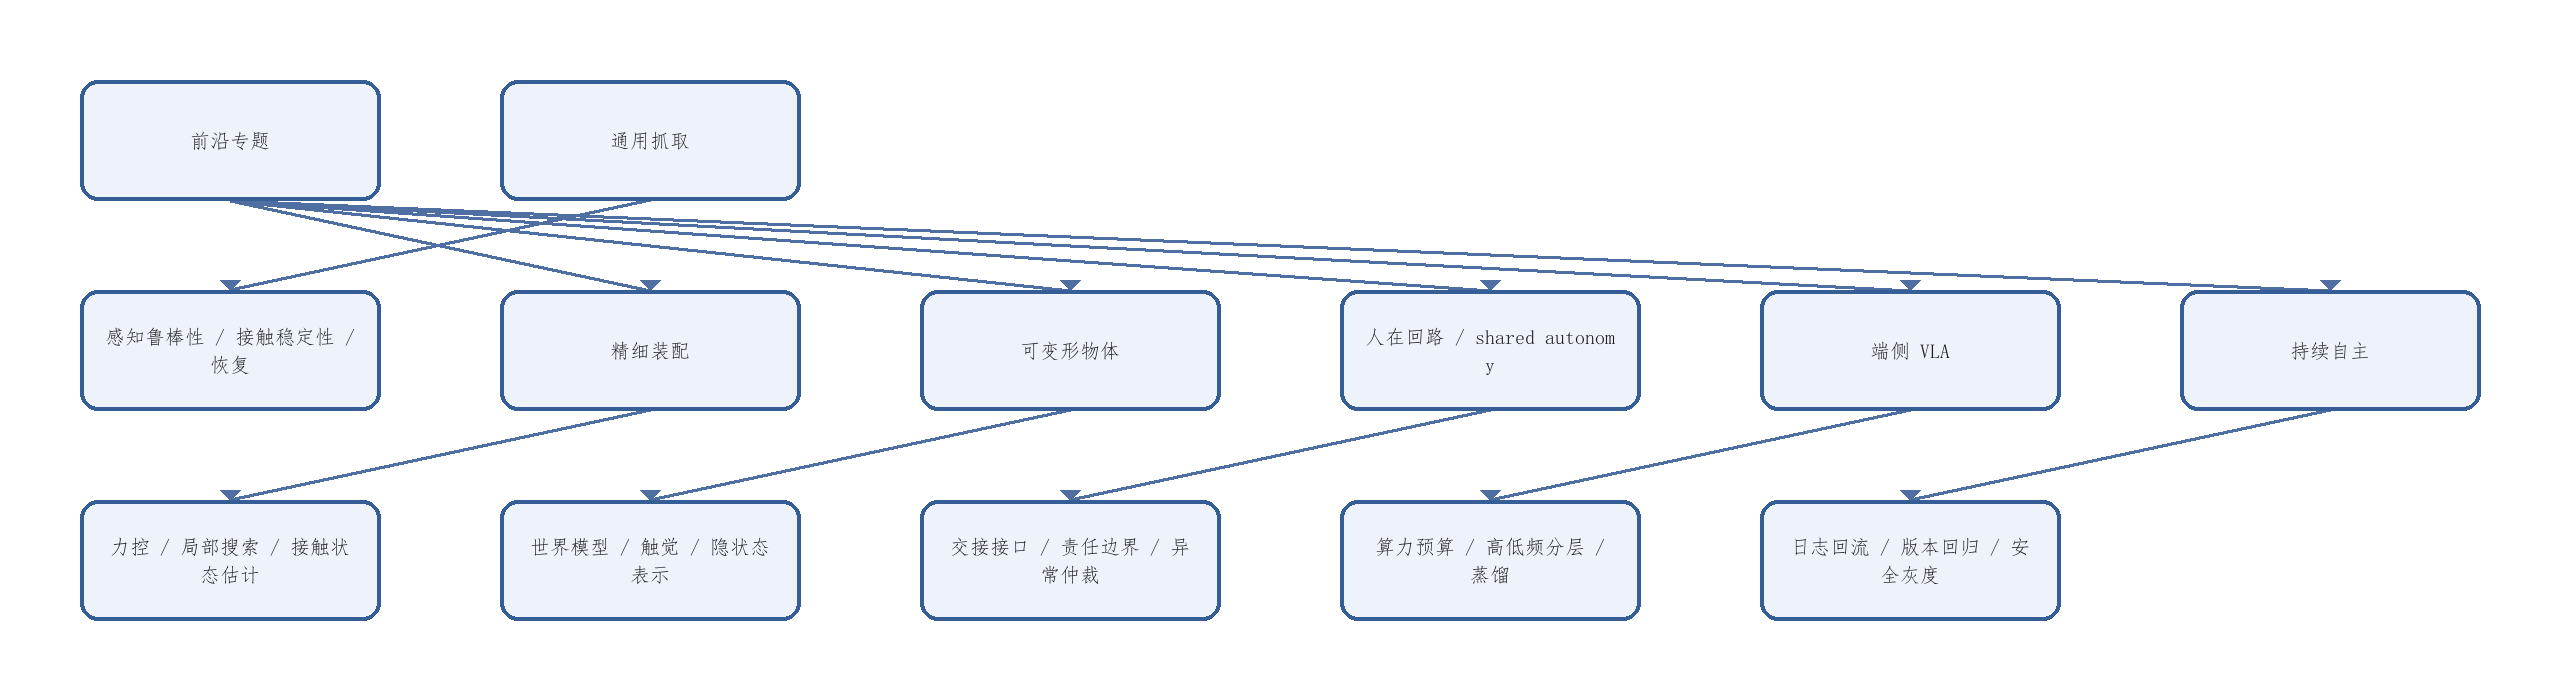
\includegraphics[width=0.9\textwidth,height=0.72\textheight,keepaspectratio]{figures/17-前沿专题与系统瓶颈图.png}
\caption{17-前沿专题与系统瓶颈图}
\label{fig:17-前沿专题与系统瓶颈图}
\end{figure}

\section*{专题映射补充}
\addcontentsline{toc}{chapter}{专题映射补充}
\markboth{专题映射补充}{专题映射补充}

本章最适合正式补成一张“前沿专题与对应系统瓶颈”映射表。它应明确指出：通用抓取主要考验感知与接触稳定性，精细装配主要考验力控与局部搜索，软体操作主要考验世界建模与触觉，端侧 VLA 主要考验算力与分层架构，持续自主则主要考验数据回流与验证基础设施。

这样做的好处是，前沿专题就不再只是热门方向清单，而会真正成为全书技术主干上的“难点坐标图”。

\section*{表 17-1 前沿专题与对应系统瓶颈映射表}
\addcontentsline{toc}{chapter}{表 17-1 前沿专题与对应系统瓶颈映射表}
\markboth{表 17-1 前沿专题与对应系统瓶颈映射表}{表 17-1 前沿专题与对应系统瓶颈映射表}

\begingroup
\small
\begin{xltabular}{\textwidth}{YYYY}
\toprule
前沿专题 & 主要瞄准的系统瓶颈 & 为什么它重要 & 当前典型难点 \\
\midrule
\endfirsthead
\toprule
前沿专题 & 主要瞄准的系统瓶颈 & 为什么它重要 & 当前典型难点 \\
\midrule
\endhead
通用抓取 & 感知-接触-恢复之间的闭环稳定性 & 是多数复杂操作能力的最小入口 & 遮挡、材质变化、抓取后滑移与重抓 \\
精细装配 & 局部搜索、力控、接触状态估计 & 能最直接暴露“会做任务”与“能稳定做成任务”的差距 & 公差小、力位协同难、失败代价高 \\
可变形物体操作 & 高维状态表示与接触预测 & 迫使系统超越刚体近似 & 状态难定义、视觉不足、接触后果复杂 \\
双臂与多指协同 & 多执行器协调与任务分工 & 接近真实复杂作业的必要前提 & 时序协调、空间互扰、接触分配 \\
端侧 VLA & 算力预算与高低频分层组织 & 决定高层模型是否能进入真实部署链路 & 延迟、热设计、模型压缩与异步调度 \\
持续自主 & 数据回流、版本回归与安全更新 & 决定系统是否能越用越强而非越改越乱 & 样本筛选、自动标注、灰度发布与回滚 \\
人在回路 / shared autonomy & 高风险场景下的责任与价值闭环 & 是许多现实行业先落地的组织形态 & 接管边界、界面设计、责任划分与 SLA \\
\bottomrule
\end{xltabular}
\endgroup

% Generated from 18-代表性论文与模型谱系梳理.md; edit the LaTeX source after migration.

\reportpart{第十八部分 代表性论文与模型谱系梳理}
\addcontentsline{toc}{part}{第十八部分 代表性论文与模型谱系梳理}
\markboth{第十八部分 代表性论文与模型谱系梳理}{第十八部分 代表性论文与模型谱系梳理}

长篇报告如果只在各章局部引用论文，很容易缺少全局脉络。因此，本部分的作用不是重复前文，而是建立一张可长期维护的谱系图：哪些路线从经典模仿学习和 RL 演化而来，哪些路线推动了 Transformer policy 与 VLA，哪些路线把世界模型与抽象预测推上前台，哪些是 2025-2026 年值得持续跟踪的新分支。

本章的一个核心目的，是把“论文列表”变成“研究地图”。也就是说，重要的不只是记住某篇论文做了什么，而是理解它在一条主线上的位置：它解决了哪个旧瓶颈，引入了什么新接口，又把问题重新推向了哪里。只有这样，这份报告后续每次增量更新时，新增论文才有机会被放回结构之中，而不是不断堆叠零散新名词。

\section*{86. 经典起点与过渡阶段}
\addcontentsline{toc}{chapter}{86. 经典起点与过渡阶段}
\markboth{86. 经典起点与过渡阶段}{86. 经典起点与过渡阶段}

\subsection*{86.1 传统模仿学习与 RL 代表工作}
\addcontentsline{toc}{section}{86.1 传统模仿学习与 RL 代表工作}


如果从今天回看，这一节最重要的价值并不只是列出若干“早期经典”，而是把具身学习最顽固的底层约束重新摆到台面上。模仿学习与 RL 时代已经把几个问题暴露得非常清楚：示教分布与闭环执行分布天然错位，真实世界试错昂贵，奖励设计脆弱，恢复能力难学，失败样本往往比成功样本更能决定系统上限。后来的 VLA、通用策略和机器人基础模型并没有让这些问题消失，而只是用更大规模的数据工程、模型参数和训练基础设施重新包装了它们。

也因此，本节不应被当成“背景材料”读过就算。更准确的理解是：这一批工作定义了后续所有路线都绕不开的共用问题空间。若不先理解这些老问题，读者就很容易把今天某些模型的阶段性成功误判成结构性突破，而忽略它们仍然在和同一组约束持续搏斗。

把这组工作放在谱系起点，最重要的不是怀旧，而是提醒后文所有“新路线”都没有脱离这些早期问题设定：示教如何进入策略、回报如何驱动优化、真实世界试错为何昂贵、恢复能力为何难学。这一谱系奠定的是问题语言，而不只是若干旧算法名称。相关代表性论文可参见 \href{https://proceedings.mlr.press/v15/ross11a.html}{DAgger}、\href{https://arxiv.org/abs/1504.00702}{《End-to-End Training of Deep Visuomotor Policies》} 与 \href{https://arxiv.org/abs/1806.10293}{QT-Opt}。

若把这一路线压成两个最基本的优化目标，那么传统模仿学习与 RL 的差别可以写成：

\begingroup
\footnotesize
\begin{equation*}
\min_{\pi}\ \mathbb{E}_{(s,a)\sim \mathcal{D}_{\text{demo}}}\big[-\log \pi(a\mid s)\big]
\end{equation*}
\endgroup

\begingroup
\footnotesize
\begin{equation*}
\max_{\pi}\ \mathbb{E}_{\pi}\!\left[\sum_{t=0}^{T}\gamma^t r_t\right]
\end{equation*}
\endgroup

前者把策略学习看成“尽量模仿已有专家轨迹”，后者把策略学习看成“通过试错最大化长期回报”。这两个目标在后来几乎所有机器人基础模型里都以改头换面的形式继续存在：行为克隆变成大规模示教预训练，RL 变成后训练、偏好校准或约束优化。因此，读这段谱系时最值得记住的不是算法名称，而是这两个目标函数之间的长期张力。

从系统责任角度看，传统模仿学习路线更容易得到“起步像样、出分较快”的策略，因为它直接消费现成专家行为；但它常常被示教分布覆盖范围严格约束，一旦离开熟悉状态就容易错误累积。RL 路线则更有机会学到恢复动作和长期信用分配，但其代价是试错昂贵、奖励脆弱、训练极不稳定。后来的大模型路线之所以不断回到“预训练 + 少量在线校正”或“示教 + 偏好 + 约束后训练”，本质上就是在这两种早期问题设定之间重新找折中点。

因此，这一谱系对后文最重要的提醒是：只要系统还要在真实物理世界中行动，就永远绕不开三个老问题。第一，如何让离线数据覆盖闭环执行时会遇到的偏离；第二，如何在代价可接受的前提下获得恢复能力；第三，如何让优化目标既不过度依赖脆弱奖励，也不完全受限于示教边界。任何后来路线若声称自己“突破了旧范式”，都值得先对照这三问重新检查。

\subsection*{86.2 Transformer policy 的早期路线}
\addcontentsline{toc}{section}{86.2 Transformer policy 的早期路线}


这一谱系的重要意义，不只是“Transformer 也能做机器人”，而是它把机器人策略学习重新组织成统一序列接口问题。状态、图像、动作、回报乃至任务条件，都开始可以被放入同一时序建模框架中比较。这样一来，模仿学习、离线 RL 和多任务策略建模之间原本较分散的接口开始被重新统一。

若把这条早期路线压缩成一个最小抽象，其核心是：

\begin{equation*}
p_\theta(y_{1:T}\mid c_{1:T})
\end{equation*}

其中 \(c_{1:T}\) 可以是状态、图像、语言、回报或任务标签，\(y_{1:T}\) 可以是动作、动作块或下一步决策标记。这个表达式看起来很一般，却有一个关键后果：机器人决策第一次被系统性改写成“序列建模接口设计”问题，而不再只是单步控制器拟合问题。

Transformer 进入机器人后，重点不是简单替代循环网络，而是把状态、动作和历史上下文放进更一般的序列接口中。这条线可以用三个代表节点来理解：

\begin{enumerate}
\item \href{https://arxiv.org/abs/2106.01345}{Decision Transformer：回报条件序列决策}。它把离线强化学习重写成“条件于目标回报的序列决策”。
\item \href{https://arxiv.org/abs/2205.06175}{Gato：通用多任务智能体}。它把跨模态多任务智能体压成统一标记流。
\item \href{https://arxiv.org/abs/2212.06817}{RT-1：机器人 Transformer 策略}。它则把这种统一接口进一步落到真实机器人多任务策略学习上。
\end{enumerate}

三者虽然经常被并排提起，但真正重要的不是名字并列，而是它们依次推动了“回报条件化”“多模态统一序列化”和“真实机器人动作接口化”这三步演化。

也就是说，这条谱系真正重要的不是“模型架构相似”，而是它连续回答了三个问题：第一，机器人决策能否像语言一样用统一序列接口表达；第二，不同模态和不同任务能否进入同一上下文；第三，这种接口能否承接真实机器人数据而不是只停留在抽象智能体层。没有这一步，后来的 VLA 与通用策略很难自然接上语言、视觉和动作的统一建模叙事。

从学习路径上看，这条早期路线还提供了一个很重要的判断模板：后续任何自称“机器人基础模型”的工作，都至少要回答它在这三个问题上的位置。它是更接近回报条件策略、统一多模态智能体，还是面向真实机器人动作接口的多任务序列模型？只有先把这层谱系位置厘清，后续比较才不会变成“谁的参数更多、谁的视频更惊艳”的表面竞赛。

\subsection*{86.3 世界模型与生成控制早期路线}
\addcontentsline{toc}{section}{86.3 世界模型与生成控制早期路线}


这一条谱系真正值得强调的，不只是它在历史上更早提出了潜在动力学、想象式轨迹展开或基于模型的学习，而是它系统性地反驳了一个偷懒想法：机器人不可能永远只靠“观测到动作”的直接映射去解决所有问题。只要任务存在多步后果、昂贵试错、接触不确定性或长时程依赖，系统就会不断被迫引入某种“内部对未来的表示”。早期世界模型路线的重要性，正在于它把这种内部表示重新变成正当研究对象。

不过，早期世界模型工作的启发不应被误读为“后来的视频世界模型已经被早早证明可行”。更准确的说法是：它们证明了学习内部环境模型有潜在高回报，但也同时暴露了模型偏差、rollout 漂移和真实接触任务中误差快速累积的问题。后来的所有世界模型热潮，都是在继承同一个愿望，也在继承同一个老难题。

这一路线的早期工作之所以值得单列，是因为它较早回答了一个今天仍然关键的问题：机器人是否可以先学一个内部环境模型，再借此做策略优化或规划，而不必每次都在真实世界中昂贵试错。后来的视频世界模型、抽象预测与可控生成路线，很多都可以回溯到这里的思想源头。相关代表性论文可参见 \href{https://arxiv.org/abs/1803.10122}{World Models} 与 \href{https://arxiv.org/abs/1912.01603}{Dreamer}。

如果把这一类方法压成最小形式，它们通常都包含一个潜状态动力学与一个基于潜状态的价值或奖励头：

\begingroup
\footnotesize
\begin{equation*}
z_{t+1}=f_{\phi}(z_t,a_t),\qquad
\hat r_t=g_{\phi}(z_t,a_t)
\end{equation*}
\endgroup

随后策略不再只在真实环境里试错，而是部分依赖 \(f_{\phi}\) 所定义的内部想象轨迹进行优化。这一重写的意义非常大，因为它第一次把“未来会怎样”正式写进了策略学习接口，而不是让策略永远只从当前观测直接映射到动作。

但也正是在这里，世界模型路线把自己的长期难点暴露得非常清楚。模型一旦有偏差，rollout 深度越长，偏差就越可能被递归放大。若把单步建模误差近似记为 \(\epsilon_1\)，则多步展开后的误差常常会呈现近似累积：

\begin{equation*}
\epsilon_H \approx \sum_{k=0}^{H-1} L^{k}\epsilon_1
\end{equation*}

其中 \(L\) 表示潜在动力学对误差的放大系数。这个式子的价值不在于精确，而在于它提醒我们：世界模型路线的关键不只是“能否预测”，更是“预测误差是否会在规划地平线内失控”。后来的视频世界模型和抽象预测路线，本质上都在继续和这个问题搏斗。

因此，早期世界模型工作的真正历史作用，是把“内部未来表示”从一个可疑想法变成了后续所有具身预测路线的共同问题设定，同时也把“模型偏差、接触误差和长时程漂移”这三个老难题一并传了下去。后文阅读任何生成式控制或视频世界模型工作时，都应追问它究竟是解决了这些难点，还是只是把同样的问题换了一个更现代的表征空间重新表达。

\section*{87. VLA 谱系}
\addcontentsline{toc}{chapter}{87. VLA 谱系}
\markboth{87. VLA 谱系}{87. VLA 谱系}

\subsection*{87.1 RT-1 / RT-2 / RT-X}
\addcontentsline{toc}{section}{87.1 RT-1 / RT-2 / RT-X}


这一组工作不应只被当作三篇论文，而应被视为同一条研究主线的连续推进：从多任务机器人 Transformer，到把互联网级视觉语言知识显式迁移到动作接口，再到跨平台数据组织与通才策略训练基础设施。它们共同回答的是一个核心问题：机器人动作建模能否像大模型那样，走向统一的多任务规模化训练接口。

若把这条路线的最小训练目标写出来，可以粗略表示为：

\begingroup
\footnotesize
\begin{equation*}
\max_{\theta} \sum_t \log p_{\theta}(a_t \mid o_{\le t}, x_{\le t}, l)
\end{equation*}
\endgroup

其中 \(o_{\le t}\) 是感知历史，\(x_{\le t}\) 是机器人状态历史，\(l\) 是语言或任务条件，\(a_t\) 则可能是离散动作标记、动作块或低层控制接口。这一写法的关键，在于它把“机器人策略学习”重写成了条件序列建模问题。

沿这条主线看，\href{https://arxiv.org/abs/2212.06817}{RT-1：多任务机器人策略} 的贡献主要在于证明多任务 Transformer 可以在统一动作词表上吸收多任务真机示教；\href{https://arxiv.org/abs/2307.15818}{RT-2：语义知识迁移到动作接口} 则进一步把互联网语义知识显式接入机器人动作接口，使“看懂世界”与“在世界里行动”开始共享一部分表征基础；到了 \href{https://arxiv.org/abs/2310.08864}{Open X-Embodiment：跨机构多本体数据协作}，焦点又被推向数据层与平台层，即跨机构、跨本体的数据是否可以被组织成训练通才策略的公共基座。

这条谱系最值得保留的，不是某篇论文的性能数字，而是一条连续可观察的接口演化链：从单本体多任务，到语义知识迁移，再到多本体、多机构数据汇聚。后文凡是出现“通用 VLA”“基础模型机器人”“跨本体迁移”等叙事，几乎都能回接到这条链条。

\subsection*{87.2 PaLM-E}
\addcontentsline{toc}{section}{87.2 PaLM-E}


PaLM-E 的标志性价值，在于它更明确地展示了“把通用多模态语言模型接入具身感知与任务执行接口”的路线。它不是最纯粹的机器人策略模型，而更像一个把语言、视觉和机器人状态共同塞进大模型上下文中的桥梁型系统，因此在谱系中承担的是“接口扩张者”的角色。

如果用极简形式表达，它所推动的问题设定更接近：

\begingroup
\scriptsize
\begin{equation*}
h_t = \mathrm{LM}_{\theta}\!\left([x^{\text{text}};\ x^{\text{vision}};\ x^{\text{state}}]\right)
\end{equation*}
\endgroup

也就是说，机器人状态不再被看成必须由传统控制模块单独消化的内部变量，而是被纳入统一上下文，与文本和视觉一起交给大模型处理。\href{https://arxiv.org/abs/2303.03378}{PaLM-E} 的历史意义，正在于它明确把“机器人状态进入大模型上下文”写成了一个正式问题，而不是工程拼接技巧。

从谱系角度看，这个改变的重要性甚至不亚于一次性能提升。它改变了后续研究者对具身多模态模型边界的想象，使得状态、任务和感知不再被默认拆成彼此孤立的系统部件。后来的许多 VLA、世界模型和任务规划接口工作，本质上都在继续回答 PaLM-E 打开的那个问题：哪些状态应该被语言模型消费，哪些又必须留在低层控制闭环里。

更重要的是，PaLM-E 让“机器人状态是否应被 token 化后交给大模型主干消费”成为了一个正式研究问题。此前大量机器人系统默认把状态留在控制模块内部，不把它视为通用推理上下文的一部分；而 PaLM-E 明确展示了另一种路线，即让状态、视觉与语言共同参与高层表征组织。后来的许多 VLA 和任务级机器人模型，无论是否完全沿用其实现细节，都在继续继承这个接口立场。

但也正因为如此，PaLM-E 的能力边界同样需要被读清楚。它更擅长回答“如何把多模态上下文接入统一语义主干”，却没有直接解决高频动作控制、接触稳定性和现场低时延部署等问题。换句话说，它在谱系中更像接口组织者而不是低层执行者。若把它误读成“已经把机器人控制本身统一到语言模型里”，就会高估其系统职责，也会误判后来 VLA 路线为何仍需要独立动作头、技能层或局部控制层。

因此，PaLM-E 在本报告中的阅读姿势不应是“看它赢了多少机器人基准”，而应是“看它如何把机器人状态带入了统一多模态主干”。它最值得长期保留的，不是某个分数，而是它替后来研究者打开的接口问题：状态究竟在哪一层被消费，消费之后又该如何与低层执行责任重新分界。

\subsection*{87.3 OpenVLA}
\addcontentsline{toc}{section}{87.3 OpenVLA}


在谱系里，OpenVLA 的价值主要体现在“把 VLA 从概念与演示，推进到更可审视的开放接口”。按照其论文表述，OpenVLA 采用约 7B 参数规模，并建立在接近 97 万条真实机器人示教轨迹之上，同时强调可以在消费级 GPU 上通过 LoRA 微调并复现主要实验 \href{https://arxiv.org/abs/2406.09246}{OpenVLA}。这使它的重要性既在模型，也在方法学透明度。

更关键的是，OpenVLA 让社区第一次较完整地看到，一个可研究、可复核的 VLA 栈至少应该暴露哪些层：

\begingroup
\scriptsize
\begin{equation*}
\text{OpenVLA Stack} = (\text{dataset protocol},\ \text{policy checkpoint},\ \text{adaptation path},\ \text{evaluation recipe},\ \text{deployment interface})
\end{equation*}
\endgroup

这个五元组的重要意义，在于它把“VLA 是一个模型”改写成“VLA 是一套协议”。很多闭源系统也许在能力上更强，但若不公开数据组织方式、动作接口、适配路径和评测口径，研究共同体就很难真正比较它们到底改写了什么问题。

对研究共同体而言，OpenVLA 的关键贡献并不是简单“做出一个开源 VLA”，而是把若干原本只存在于闭源系统中的核心问题重新拉回公共空间：训练样本长什么样、动作表示怎么定义、推理流程如何组织、评测口径如何设置、部署时需要暴露哪些接口。换句话说，它建立了后续路线比较的公共参考面。

因此，在长期维护谱系时，OpenVLA 这一节点的重要性不只来自模型本身，而来自它提供了一个对社区可见、可修改、可复审的坐标点。很多后续工作未必直接继承其全部设计，但会借它重新定义“一个 VLA 系统至少应公开哪些接口”，这对开源生态和研究复核都极其关键。

从这份报告的角度看，OpenVLA 还承担了一个教学上的枢纽角色：它把第 11 章的动作接口、第 13 章的数据组织和第 19 章的开源工具链串成了一条可以被读者真正沿着走通的学习路径。也正因为如此，它在谱系图中的位置不只是“一个模型名称”，而更像是“开源 VLA 方法论开始成形”的标志节点。

\subsection*{87.4 SmolVLA 与轻量路线}
\addcontentsline{toc}{section}{87.4 SmolVLA 与轻量路线}


SmolVLA 与轻量路线值得单列，不只是因为参数更小，而是因为它把一个常被后置的问题提前到了研究主线里：若具身系统最终必须跑在功耗、时延和维护预算都受限的端侧环境，那么“缩小模型并尽量保住关键能力”就不是部署优化，而是模型路线本身的一部分。

这类路线通常同时压缩三个维度。第一是参数规模与推理路径长度，避免每次动作生成都依赖高昂前向计算；第二是输入输出接口复杂度，例如更紧凑地表达动作块或减少不必要的高分辨率模态；第三是训练与蒸馏方式，让小模型继承大模型学到的语义先验，而不是要求它从头吸收全部能力。轻量化若只做第一层而忽略后两层，往往会得到一个“更小但仍然不适合部署”的模型。

\href{https://arxiv.org/abs/2506.01844}{SmolVLA} 的价值正在于此。它不是单纯把大模型裁小，而是把轻量部署、社区数据、异步推理栈和 Hugging Face 生态一起纳入设计目标。这说明“轻量化”已经从后处理技巧，变成了路线级问题设定。

因此，轻量路线不是“大模型路线的附属优化”，而是与“更大模型”并行存在的一条主线。只要真实部署持续受到端侧算力、热设计功耗和维护成本约束，轻量 VLA 就不会只是妥协方案，而会长期成为大规模可部署系统的核心候选。

从谱系比较角度看，轻量路线真正改变的是评价顺序。传统读法常把“先看谁性能更高，再看能否压缩”；而轻量路线要求反过来先问“部署预算是什么”，再问“在该预算下还能保住哪些关键能力”。这会把模型设计直接拉回控制频率、显存占用、异步推理延迟、动作块长度和失败恢复策略等工程变量上。也因此，SmolVLA 之类工作对报告的价值，不在于它们是否取得了绝对最强性能，而在于它们把“部署友好性”提前写成了问题定义的一部分。

这条路线还有一个长期意义：它更容易形成可复现社区协议。超大模型路线往往需要闭源数据、专有基础设施或企业级算力，而轻量路线更容易让研究社区通过单卡训练、端侧推理和开源工具链建立公共实验基线。若后续版本要长期跟踪“哪些路线更可能形成公共生态”，轻量 VLA 往往比单纯更大模型更值得持续观察。

当然，轻量路线也有自己的负空间。它往往更早暴露上下文长度、动作细粒度、视觉分辨率和恢复策略上的取舍，因此不应被误读成“更小但几乎没有代价”。更准确的理解是：它把这些代价显式写进了问题定义，使研究者无法再把部署问题无限后置。

\section*{88. 世界模型与 JEPA 谱系}
\addcontentsline{toc}{chapter}{88. 世界模型与 JEPA 谱系}
\markboth{88. 世界模型与 JEPA 谱系}{88. 世界模型与 JEPA 谱系}

\subsection*{88.1 视频世界模型}
\addcontentsline{toc}{section}{88.1 视频世界模型}


视频世界模型路线之所以在近两年如此醒目，一个核心原因是它把“预测未来”重新做成了高度可视化、跨学科都能直观看懂的研究对象。对机器人而言，这种表达有明显吸引力：如果模型能够根据当前观察、动作历史和任务条件生成未来视频，那么它似乎就有机会同时承担前瞻感知、风险评估、候选轨迹筛选和失败预警等多个角色。

但恰恰因为它可视化很强，也更容易掩盖真正的控制需求。机器人并不需要“看起来像真的未来”，而更需要“对行动成败有用的未来”。一个更接近机器人使用方式的抽象是：

\begin{equation*}
z_{t+1:t+H} = f_{\phi}(z_t,\ a_{t:t+H-1},\ g)
\end{equation*}

这里 \(z\) 不一定是像素，也可以是潜状态、对象关系或可规划结构。关键问题不在于视频是否逼真，而在于这些未来表示能否帮助系统判断接触是否建立、碰撞是否会发生、动作是否会破坏后续操作空间。若回答不了这些问题，视频世界模型在具身闭环中的价值依然有限。

从系统角度看，视频世界模型真正可能服务于三类接口：第一，作为候选动作的风险预筛器；第二，作为遮挡或不完全观测下的未来补全器；第三，作为长时程任务中的阶段进展预测器。若它不能进入这三类接口中的任意一种，而只是独立生成“看起来合理”的视频，那么它在机器人系统里的位置仍更接近分析工具，而不是决策部件。

这一路线的典型失败模式也必须被一并写清楚。第一类失败是视觉逼真但物理不真，即生成结果表面连贯，却不保留接触约束、惯性后果或碰撞逻辑；第二类失败是对决策无关，即视频很像未来，却无法帮助系统区分“该抓还是该绕开”；第三类失败是 rollout 累积漂移，即短期几帧看似合理，长时程预测却迅速失真。若不把这些失败模式单独记下，读者就很容易把“视频生成更强”误读为“机器人更会行动”。

因此，本节讨论视频世界模型时，重点不应放在生成质量本身，而应放在它是否进入了真实决策接口。它在谱系中的位置，更像“开放世界未来表达能力的推进器”，而不是已经完成闭环落地的控制替代物。

\subsection*{88.2 抽象预测路线}
\addcontentsline{toc}{section}{88.2 抽象预测路线}


抽象预测路线的重要性，在于它改变了“什么才值得预测”的答案。与逐像素重建不同，这一路线更强调预测对任务真正有用的结构，例如对象关系、接触阶段、拓扑变化、潜在状态迁移或高层语义约束。对机器人而言，这种转向尤其关键，因为机器人最终消费的不是好看的画面，而是足以支撑规划、约束检查和技能调用的可执行结构。

JEPA 及相关路线的核心思想，是不必重建全部像素，只需预测足够有用的抽象结构 \href{https://arxiv.org/abs/2301.08243}{JEPA}。若写成极简形式，可以表示为：

\begin{equation*}
\hat z_{\text{target}} = g_{\phi}(z_{\text{context}})
\end{equation*}

其中被预测的是“对任务有意义的表征”，而不是像素级未来。需要强调的是，JEPA 本身并不是机器人专用方法；这里把它纳入谱系，主要是因为它提供了一种方法论立场：对具身系统真正重要的，未必是把未来画得更真，而是把对任务、控制和预测有用的结构保留下来。

从工程视角看，抽象预测的优势也更明显。它更容易与任务规划器、技能库、约束求解器、安全监测器和状态机对接，因为这些模块本来就偏好结构化变量而不是原始像素。但其挑战同样不小：什么样的抽象才足够通用，如何保证抽象变量对真实接触后果敏感，以及如何避免学到“看似稳定却对控制无用”的潜空间，仍然是未解决的问题。

这一路线对后续机器人研究最重要的启发，是把“预测什么”从一个视觉 fidelity 问题改写成接口设计问题。若后续消费模块是技能检索器、约束检查器或任务规划器，那么理想抽象应优先保留对象关系、接触阶段、可达性和风险边界，而不是优先保留像素纹理。也就是说，抽象预测路线并不是天然更高级，而是更明确地承认：预测目标必须服务于后续决策接口。

但这条路线也有独特风险。抽象一旦定义得过粗，系统会得到一个稳定却无用的潜空间；抽象一旦定义得过窄，又会快速绑定到特定任务或本体，失去通用性。因此，后续判断任何“抽象预测成功”工作时，都应同时检查两件事：其抽象是否真的被后续策略或规划消费，以及这种抽象是否在跨场景或跨任务时仍保持解释力。否则，所谓抽象优势很可能只是在单一基准上的局部工程胜利。

因此，抽象预测路线最适合与后文的世界接口和规划接口一起读，而不适合孤立地只和像素指标比较。只要一种抽象无法稳定进入技能调用、约束检查或长期记忆写入，它即使看起来更“语义化”，对具身系统的主链条价值也仍然有限。

\subsection*{88.3 可控生成与规划结合路线}
\addcontentsline{toc}{section}{88.3 可控生成与规划结合路线}


这一节最值得强调的一点是：可控生成真正改变的，不是生成模型“会不会画未来”，而是它开始尝试承担行动候选提议器的角色。系统不再只做一次前向传播直接给出动作，而更像是先生成若干可选轨迹、子目标或技能序列，再由约束检查、价值评估、碰撞检测或外部规则进行筛选。这种组织方式比纯端到端策略更接近许多真实机器人系统的工作逻辑。

若写成统一的选择形式，可以表示为：

\begingroup
\scriptsize
\begin{equation*}
a^{*}_{t:t+H-1} =
\arg\max_{a_{t:t+H-1}}
U\!\left(f_{\phi}(z_t, a_{t:t+H-1}),\ g,\ \mathcal{C}\right)
\end{equation*}
\endgroup

其中 \(f_{\phi}\) 给出未来表征或候选轨迹展开，\(U\) 则综合任务目标 \(g\) 与约束集合 \(\mathcal{C}\) 来做筛选。关键不在于生成本身，而在于生成接口是否能被价值函数、约束检查器和恢复逻辑稳定消费。

当然，生成与筛选的组合并不会自动带来可靠性。候选过多会导致搜索成本上升，候选过少又失去规划收益；而一旦筛选器本身带有偏差，系统还可能稳定偏好“看似分高、现实会失败”的解。也因此，这条谱系的长期潜力不只取决于生成模型本身，还取决于生成接口与评估接口能否同步成熟。

从更贴近系统工程的角度看，这条路线实际上把决策分成了两个责任层。生成模型负责提出若干“可能有戏”的未来候选，外部评估器负责决定哪些候选在任务、几何、接触和安全约束下仍值得继续推进。二者若缺一，系统都会出问题：没有生成器，系统只能在固定技能库里做局部搜索；没有评估器，系统又会被“看起来合理”的伪候选牵着走。

因此，这一谱系最值得长期跟踪的不是某一个候选生成器性能分数，而是三项接口是否同步成熟。第一，候选是否足够多样且覆盖关键恢复动作；第二，评估器是否真的理解约束，而不是只偏好表面顺滑轨迹；第三，最终被选中的候选是否还能被低层执行器稳定消费。只要这三项中任一项缺位，可控生成路线就很容易沦为演示中漂亮、部署时脆弱的系统。

若后续版本继续维护这一谱系，最值得单独记录的字段不是“是否用了生成模型”，而是“候选如何产生、谁来筛选、筛选依据是否显式、执行器是否支持回退”。只有把这些字段固定下来，读者才不至于被生成式 demo 的表面流畅度牵着走。

\subsection*{88.4 谱系分歧的根本问题}
\addcontentsline{toc}{section}{88.4 谱系分歧的根本问题}


这些谱系持续分歧，根本不只是因为研究者偏好不同模型结构，而是因为它们默认的“主问题”并不相同。有的路线把核心难点定义为语义对齐，认为只要互联网级视觉语言知识能成功接到机器人动作接口上，能力上限就会迅速上升；有的路线把关键问题定义为接触与恢复，认为真正限制部署的是物理交互中的长尾异常；还有的路线把焦点放在系统组织，认为数据采集、仿真、评测与运维闭环才是决定谁能长期迭代的关键。

换言之，谱系分歧本质上对应不同目标函数。粗略地写，可以表示成：

\begingroup
\scriptsize
\begin{equation*}
\min_\theta \mathcal{L}=
\lambda_1 \mathcal{L}_{\text{semantic}}
+ \lambda_2 \mathcal{L}_{\text{control}}
+ \lambda_3 \mathcal{L}_{\text{recovery}}
+ \lambda_4 \mathcal{L}_{\text{deployment}}
\end{equation*}
\endgroup

不同路线之间并不是只在求解器或骨干结构上不同，而是连 \(\lambda_i\) 的权重都不同。这也是为什么很多路线很难在单一 benchmark 上得出“谁统一胜出”的结论。

对整本报告的维护来说，这一节很关键，因为它提醒我们后续版本更新时不应把所有新工作机械塞进同一条时间轴里。更好的做法，是先判断新工作究竟强化了哪一类目标函数，再把它放回对应谱系。只有把“它是为表达、为预测、为规划还是为控制服务”写清楚，谱系章节才不会随着新论文累积而失控。

\section*{89. 2025-2026 关键增量工作}
\addcontentsline{toc}{chapter}{89. 2025-2026 关键增量工作}
\markboth{89. 2025-2026 关键增量工作}{89. 2025-2026 关键增量工作}

\subsection*{89.1 GR00T N1}
\addcontentsline{toc}{section}{89.1 GR00T N1}


在谱系梳理里，GR00T N1 更适合被放在“平台化机器人基础模型”坐标中理解，而不是只看作某个单点模型。它背后捆绑了仿真、合成数据、机器人本体接口与后续部署叙事，因此其研究意义不仅来自模型能力，也来自它试图重新组织整条开发链路。\href{https://arxiv.org/abs/2503.14734}{GR00T N1} 于 2025-03-19 在 arXiv 发布，其论文摘要就明确强调了异构数据整合、双系统架构和面向人形的通用自治。

GR00T N1 的谱系地位之所以值得单列，是因为它把“模型能力”与“平台组织能力”重新绑到一起。若把这一类路线的真正主张写成一个最小面板，更接近：

\begingroup
\scriptsize
\begin{equation*}
\text{Platform Route} = (\text{foundation model},\ \text{simulation},\ \text{synthetic data},\ \text{embodiment adapters},\ \text{runtime stack})
\end{equation*}
\endgroup

这里真正值得长期追踪的，并不是其中某一项是否最强，而是它们是否被组织成了一条足以缩短闭环周期的协同链。若模型很强、仿真很强、数据也很多，但这些能力彼此并未形成可复用默认工作流，那么平台化叙事就仍然停留在拼图层，而不是基础设施层。

对这条路线，更值得追问的不是“它是不是又一个大模型”，而是三件事。第一，它的输入输出接口是否真的适合跨本体复用，而不是仍隐含大量特定机器人先验。第二，它是否建立了足够可迁移的数据与评测语言，使更多团队可以围绕同一栈协作。第三，它在端侧部署、恢复和监控上究竟回答了多少问题，而不是只在训练与演示层面给出愿景。

因此，GR00T N1 的谱系意义在于：平台型公司开始更主动地定义“机器人基础设施层”的边界，而不只是发布单点模型。对行业分析来说，这通常意味着竞争重心正在从“谁有更强单点模型”，转向“谁能把模型、数据、仿真与本体接口组织成默认工作流节点”。

\subsection*{89.2 Gemini Robotics / On-Device}
\addcontentsline{toc}{section}{89.2 Gemini Robotics / On-Device}


把 Gemini Robotics / On-Device 单列出来很重要，因为它代表的不只是“更强模型”，还代表另一条趋势：高能力模型是否能够进一步压缩、拆层或重组，进入更贴近端侧与现场的运行模式。这条路线与纯云端大模型叙事并不完全相同。

Google DeepMind 在 2025-03-12 发布 \href{https://deepmind.google/discover/blog/gemini-robotics-brings-ai-into-the-physical-world/}{《Gemini Robotics》官方博客}，把其机器人能力概括为通用性、交互性与灵巧性；又在 2025-06-24 发布 \href{https://deepmind.google/discover/blog/gemini-robotics-on-device-brings-ai-to-local-robotic-devices/}{《Gemini Robotics On-Device》官方博客}，明确把本地运行、低时延与少量样本适配提到前台。这个时间顺序本身就很关键：先证明“通用多模态模型能进入物理世界”，再证明“这种能力必须被重新组织成现场可运行形态”。

从谱系意义看，这条路线把通用多模态模型阵营与机器人问题设定更直接连接起来，同时把端侧约束显式提到前台。这意味着“通用模型进入物理世界”不再只是概念叙事，而开始变成接口与部署问题：哪些语义能力该留在高层，哪些动作接口必须局部执行，哪些能力必须为低时延牺牲通用性。

若把这一路线进一步压成一个责任分层判断，它更接近：

\begingroup
\footnotesize
\begin{equation*}
\pi_{\text{system}}
=
\pi_{\text{high-semantic}}
\circ
\pi_{\text{local-real-time}}
\end{equation*}
\endgroup

也就是说，系统并不是把整套推理都塞进一个统一运行时，而是重新划分“哪些能力可以慢一点但更通用，哪些能力必须快一点但更局部”。这正是 On-Device 版本真正重要的地方：它把部署责任从“云端有多强”转回到“本地还能留下多少可用能力”。

因此，这一路线的长期价值并不只是证明 Gemini 能做机器人，而在于它把“通用多模态底座如何切分为高层语义与端侧执行能力”正式摆到主线里。后续判断相关工作时，不应只看 demo 中展示了多少任务，更应追问其本地运行部分到底承担了哪些职责、牺牲了哪些能力、又换来了哪些稳定性与时延收益。

从谱系阅读方法上说，Gemini Robotics / On-Device 更适合被当成“责任重划分样本”而不是“万能新模型”。它的真正研究意义，在于把模型能力、运行位置和现场时延要求重新绑在一起讨论，这一点对后文硬件、部署与端侧路线的判断尤为关键。

\subsection*{89.3 Figure Helix}
\addcontentsline{toc}{section}{89.3 Figure Helix}


Figure Helix 在谱系中的意义，更适合理解为“企业级系统整合路线的公开化片段”。它提供的往往不是完整开源方法，而是一个观察窗口，让我们看到企业如何把语言、规划、技能执行和本体系统耦合到一起。

\href{https://www.figure.ai/news/helix}{Figure Helix} 于 2025-02-20 公布，其最值得记录的不是营销叙事，而是公开给出了高低频双系统结构：高层视觉语言模型以约 7-9 Hz 运行，低层本体控制以 200 Hz 闭环运行，并且强调使用少量车载 GPU、整身上半身控制和数百小时高质量遥操作数据。这使 Helix 不只是“公司新闻”，而是一个很明确的系统架构样本。

如果说 OpenVLA 更像“开放研究协议样本”，那么 Helix 更像“企业系统责任切分样本”。它告诉我们：产业界并没有普遍相信“一个超大模型直接吞掉整条控制栈”就足够，反而更倾向于把高层语义推理、动作组织和低层连续控制放在不同时间尺度上协同。

因此，Helix 在谱系上的独特价值，不只是模型名字，而是它把以下三个问题公开得比许多企业案例更清楚：

\begin{enumerate}
\item 高层模型以什么频率参与决策，而不是持续霸占所有控制周期。
\item 低层闭环如何保留在更快、更窄、更可验证的责任层内。
\item 高质量遥操作数据与实时硬件预算如何共同决定系统边界。
\end{enumerate}

从谱系位置上看，Helix 的关键价值在于：它把高层语义推理与低层快速闭环之间的接口公开讲清楚了。这使它成为观察“高低频分层是否会成为产业主流组织方式”的重要样本，而不只是又一个企业演示案例。

\subsection*{89.4 Physical Intelligence π0 路线}
\addcontentsline{toc}{section}{89.4 Physical Intelligence π0 路线}


Physical Intelligence 的 π0 路线值得单列，是因为它代表了另一类更强调机器人基础模型化、数据组织和系统路线整合的方向。其价值不只在单篇结果，而在于它试图重新回答“通用机器人能力应如何被组织成可扩展训练对象”。\href{https://www.pi.website/blog/pi0}{π0} 于 2024-10-31 发布，虽然时间早于本节聚焦的 2025-2026，但它到 2025-2026 仍持续影响行业对“机器人基础模型”叙事的组织方式，因此这里必须保留它作为关键参照点。

从技术接口看，这类路线更愿意把机器人控制写成统一的条件动作建模对象：

\begingroup
\footnotesize
\begin{equation*}
a_{t:t+H} \sim p_{\theta}(\cdot \mid o_{\le t}, x_{\le t}, l)
\end{equation*}
\endgroup

不同之处在于，它更强调跨任务、跨本体和跨数据形态的统一组织，而不只是某个单场景最优控制器。

这类路线在谱系中的作用，还在于它们会重新命名问题并重组注意力。命名方式一旦变化，研究资源配置、企业叙事和资本理解问题的框架也会随之变化。因此，哪怕技术内核与既有路线连续，这类“重新命名问题”的工作也值得额外标注，因为它们会影响后续行业如何理解同一类能力边界。

更进一步说，π0 路线的真正关注点不是某一个单任务成绩，而是训练对象的组织方式：如何把不同机器人、本体状态、任务描述与动作输出统一进一个可扩展条件分布中。这种叙事会自然推动研究者把焦点从“某个任务上最优控制器有多强”转向“模型、数据、任务接口和本体差异是否可以被纳入同一扩展框架”。因此，它对行业理解问题空间的方式影响很大，即使具体实现后续仍可能被其他路线替代。

也正因为如此，π0 的长期价值更像“谱系重组器”而非“单次结果冠军”。它帮助行业把机器人基础模型重新理解为一套跨任务、跨本体、跨数据组织方式的联合问题。后续若出现更新路线，也很可能沿着它所强化的这几个维度继续竞争，而不是回到只比较单任务成功率的旧框架。

因此，阅读 π0 时最应避免的误判，是把它只看成“又一个条件动作模型”。更准确的看法是：它在叙事层面推动了一个更大的问题重组，即把机器人基础模型理解为模型、数据和平台协同组织的问题，而不只是单条策略曲线的竞争。

\subsection*{89.5 2026 年细分场景 VLA 论文}
\addcontentsline{toc}{section}{89.5 2026 年细分场景 VLA 论文}


把 2026 年大量细分场景 VLA 工作单独列出很有必要，因为它们共同说明了一点：行业并没有简单收敛到“一个通用 VLA 吞掉一切”，而是在动态场景、移动操作、可变形操作、端侧运行时与低成本平台上继续分化出更务实的路线。谱系梳理若不把这些分支写出来，就会高估统一范式的收敛程度。

到 2026 年上半年，这类工作至少已经沿四个方向明确分叉：

\begin{enumerate}
\item 动态场景与连续控制方向，例如 \href{https://arxiv.org/abs/2605.31286}{DynamicVLA}，重点解决动态物体、流式动作生成与长时连续推理。
\item 移动操作与规划耦合方向，例如 \href{https://arxiv.org/abs/2604.15049}{UniPlan}，显式把符号规划、VLM 与 VLA 组合到移动操作工作流里。
\item 可变形与复杂接触方向，例如 \href{https://arxiv.org/abs/2602.19201}{DeMaVLA}，把可变形物体操作与 DAgger 式持续纠偏显式拉回主线。
\item 推理运行时与部署系统方向，例如 \href{https://arxiv.org/abs/2607.00556}{Embodied.cpp}，重点不在再造新模型，而在把具身基础模型真正跑进受限硬件与统一运行时。
\end{enumerate}

这些细分场景工作在谱系里像“压力测试节点”。它们不断把“通用叙事”拉回具体本体、任务、时延和部署限制，使我们能够更早看清不同路线在真实系统条件下的边界究竟在哪里。后续新增论文时，最关键的不是它是不是又用了 VLA 名词，而是它到底在解决哪类真实约束。

\section*{90. 谱系比较框架}
\addcontentsline{toc}{chapter}{90. 谱系比较框架}
\markboth{90. 谱系比较框架}{90. 谱系比较框架}

\subsection*{90.1 输入输出范式}
\addcontentsline{toc}{section}{90.1 输入输出范式}


做跨论文比较时，输入输出范式应该首先被拉出来，因为它决定了“这些模型到底是不是在解决同一类问题”。有的模型输入图像加语言、输出单步动作；有的输入长上下文视频和状态，输出动作块；有的输入潜状态与目标，输出规划候选。若不先统一这个维度，后续比较训练规模和成功率往往没有意义。

一个更适合长期维护的做法，是把“输入输出卡”固定写成五元组：

\begingroup
\scriptsize
\begin{equation*}
\text{IOCard}=(\text{obs window},\ \text{state},\ \text{language},\ \text{action granularity},\ \text{control rate})
\end{equation*}
\endgroup

这样做的价值在于，它迫使维护者回答：输入是否包含历史窗口、是否包含本体状态、输出是单步还是动作块、输出是低层控制量还是中层技能表示、系统默认部署在什么控制频率上。只有把这些接口细节记清楚，后续才有可能判断两篇论文究竟是在同一问题上竞争，还是仅仅表面形式相似。

本章后续维护时，建议直接配合 18-论文谱系字段表 使用。先填字段，再写评价，比先写印象式评论更能保持跨版本口径稳定。

这一字段卡最容易帮助识别的一类误读，是把“都接受图像+语言输入”误判为“解决的是同一问题”。例如，一个模型若输出 1 Hz 的技能 token，另一个模型若输出 50 Hz 的连续控制块，二者即便都叫 VLA，其系统职责也完全不同。前者更接近高层任务接口，后者更接近中层动作生成器。若不把输出粒度和控制频率写清楚，就很容易把两条本该分层比较的路线放进同一排名表里。

因此，输入输出范式这一列不只是信息登记项，更是全文比较时的第一道过滤器。只要 IOCard 不同到影响职责边界，后续比较就必须谨慎降级为“相邻路线比较”，而不应继续做简单优劣排序。

在长期维护中，凡是遇到新论文或新系统，只要 IOCard 无法被快速写清楚，就说明维护者实际上还没有看懂它在系统里承担什么职责。在这种情况下，报告应优先补字段、暂缓下结论，而不是急于给出路线判断。

\subsection*{90.2 数据来源}
\addcontentsline{toc}{section}{90.2 数据来源}


数据来源必须单独比较，因为它直接决定结论能说明什么。示教数据、遥操作数据、互联网视频、仿真数据、跨平台混合数据和企业闭源现场数据，背后对应的是完全不同的接口假设与泛化边界。若不把这些差异写出来，很多横向对比都会失真。

一个更实用的做法，是把数据来源写成一张固定字段卡：

\begingroup
\scriptsize
\begin{equation*}
\text{SourceCard} = (\text{source type},\ \text{interaction level},\ \text{organization mode},\ \text{failure coverage},\ \text{rights status})
\end{equation*}
\endgroup

这里的 \texttt{\detokenize{source type}} 回答数据来自真机、遥操作、仿真还是互联网；\texttt{\detokenize{interaction level}} 回答数据是被动观察还是带真实交互后果；\texttt{\detokenize{organization mode}} 回答这些数据是单平台专用、跨平台对齐、带失败样本回流，还是经过强人工清洗；\texttt{\detokenize{failure coverage}} 回答数据是否包含偏差与恢复；\texttt{\detokenize{rights status}} 则提醒后续维护者不要忽略再训练与再分发边界。

很多论文表面上都写“多源数据训练”，但决定能力边界的，常常正是第二层和第三层。对具身系统而言，数据组织方式本身往往就是系统设计的一部分。因此，数据来源这一列不应只是背景信息，而应被视为解释变量。很多“模型 A 比模型 B 强”的结论，若不放回数据来源与采数组织方式里看，往往会被高估甚至误读。

一个典型误读是：看到某篇工作使用“更大规模数据”，便自然推断其模型路线更优。但若这些数据主要来自高一致性平台、强人工清洗或封闭遥操作接口，而对照工作使用的是跨平台但噪声更高的数据，那么结论就不能再被简单解释为“模型赢了模型”。很多时候，真正被比较的是数据组织方式、采数协议与失败覆盖率，而不是参数化策略本身。

因此，后续版本维护中，数据来源列最好被当成解释优先级很高的字段。只要 SourceCard 差异显著，正文中的性能比较就应主动降调，改写成“在不同数据制度下得到的结果差异”。这会让整本报告更接近研究判断，而不是榜单式汇总。

换句话说，SourceCard 既是比较字段，也是降噪装置。它的作用是强迫维护者在看到亮眼结果时先问：这究竟是模型更强，还是数据组织制度更有利。只要这一步没有做，后续任何“路线优劣”判断都应被视为暂定意见。

\subsection*{90.3 泛化目标}
\addcontentsline{toc}{section}{90.3 泛化目标}


泛化目标同样必须单列，因为不同论文口中的“泛化”常常不是同一件事。有的指新物体，有的指新语言描述，有的指新布局，有的指新任务组合，有的甚至指新机器人本体。报告若不把这些目标拆开，就很容易把不同强度的结论混为一谈。

为了让这类比较在后续版本中不失真，一个更实用的办法是把泛化目标固定拆成五列：

\begingroup
\scriptsize
\begin{equation*}
\text{GenCard} = (\text{semantic},\ \text{object},\ \text{environment},\ \text{recovery/time},\ \text{embodiment})
\end{equation*}
\endgroup

这样即便不同论文都使用了同一个 \texttt{\detokenize{generalization}} 术语，我们也仍能看清它们到底是在同一维度上竞争，还是只是在共享一个容易被高估的口号。比如，“换了新杯子仍能抓取”与“换了新机器人本体仍能执行同类任务”都可能被写成泛化，但它们对系统设计的要求完全不同。

这一点对阅读机器人论文尤其关键，因为“泛化”在该领域常常被过度口号化。对读者而言，更有价值的做法不是记住某篇论文声称“实现了泛化”，而是追问它究竟在哪个变量上外推：是换了未见物体但仍在相同桌面与相同夹爪上，还是换了相机布局、换了任务组合、甚至换了机器人本体。前者说明的是局部鲁棒性，后者才更接近平台级迁移。

这也是为什么泛化目标列在比较时几乎应先于总成功率。若一条路线只在 \texttt{\detokenize{object}} 维度外推，而另一条路线尝试在 \texttt{\detokenize{environment}} 与 \path{recovery/time} 同时外推，那么二者的成功率数字本来就不应直接并列。很多被媒体或社交网络渲染成“谁更通用”的争论，本质上只是没有先把泛化变量写清楚。

因此，GenCard 最重要的作用，不是制造更复杂的表格，而是强迫维护者在写评价前先回答：“这篇论文究竟在哪个变量上承担了风险？”只有把承担风险的维度写清楚，后续的好坏判断才不会被泛化这一口号轻易带偏。

这也意味着，后续读到任何“更通用”的新路线时，最稳妥的做法都不是立刻接受其摘要措辞，而是先把它填回 GenCard。只要表中仍有大量空白列，这条路线就还不足以被称为平台级泛化。

\subsection*{90.4 开源程度}
\addcontentsline{toc}{section}{90.4 开源程度}


开源程度在机器人领域之所以应被单独列为比较维度，不只是因为“能不能复现”重要，更因为它直接决定一条路线能否形成公共接口。论文级公开只能帮助外界理解主张，权重级公开只能帮助感知能力边界，而训练代码、数据协议、评测脚本、部署接口和社区维护机制的开放，才真正有机会把单篇工作变成后续研究和工程的共同底座。

更严格地说，开源程度至少可以拆成五层。第一层是论文与项目页公开，解决“外界能否知道你做了什么”；第二层是模型权重公开，解决“外界能否直接试用能力边界”；第三层是训练与推理代码公开，解决“外界能否重建方法”；第四层是数据协议、评测脚本和环境配置公开，解决“外界能否公平比较”；第五层是维护机制和 issue 响应，解决“这条路线是否真的在形成公共生态”。

在长期维护中，我更建议把它写成一个五级刻度，而不是开源/闭源二元标签：

\begin{enumerate}
\item \texttt{\detokenize{L1}}：只有论文或项目页。
\item \texttt{\detokenize{L2}}：提供权重或演示接口。
\item \texttt{\detokenize{L3}}：提供训练/推理代码。
\item \texttt{\detokenize{L4}}：连同数据协议、评测脚本和环境配置一并开放。
\item \texttt{\detokenize{L5}}：形成持续维护、社区反馈和二次开发生态。
\end{enumerate}

因此，开源程度不是“开源/闭源”二元判断，而更适合理解为一个分层变量。对学习与研究来说，真正能塑造社区演进的，往往不是单一权重是否开出，而是能否形成一套被后来者继续调用和修改的公共工作流。OpenVLA、LeRobot 这类路线之所以在本报告中权重较高，正是因为它们更接近后两层，而不是仅仅因为“公开了某篇论文的配套仓库”。

这一字段还会直接影响报告后续的研究资产沉淀方式。对于 \texttt{\detokenize{L1-L2}} 路线，更适合保留为论文卡和路线级判断；对于 \texttt{\detokenize{L3-L4}} 路线，则值得进一步沉淀为可复现的工具链、配置记录和对比表；而只有接近 \texttt{\detokenize{L5}} 的路线，才真正值得在长期版本里持续当作公共基础设施跟踪。也就是说，开源程度不只是方法学评价项，还会决定本项目后续该把多少维护预算投入到对应路线。

因此，开源程度这一列的真正作用，是把“是否值得继续跟踪”与“是否适合作为研究或工程基础设施复用”明确区分开来。很多路线学术上很重要，却未必适合成为长期可复现底座；反之，一些绝对性能未必最强的路线，可能因为开放协议更完整而更值得持续维护。这种区分，对做长期版本化报告尤其关键。

对本项目而言，OpenScore 的实用含义还在于资源分配。只有当一条路线的开放层级足以支撑后续复用时，才值得投入更多图表、代码片段和长期更新预算；否则，更合适的做法通常是保留判断、降低维护权重，而不是把有限精力投入到难以持续复现的对象上。

\subsection*{90.5 工程可部署性}
\addcontentsline{toc}{section}{90.5 工程可部署性}


工程可部署性之所以要单列，是因为很多论文方法在研究口径下成立，但并没有回答时延、恢复、监控、接管、安全冗余和运维这些部署问题。谱系梳理若不把这一维度显式写出来，就很容易把“研究亮点”误读成“可交付能力”。

一个实用比较框架可以至少看四点：

\begin{enumerate}
\item 推理时延与部署形态。
\item 是否显式讨论恢复与安全。
\item 是否依赖高度理想化本体或场景。
\item 是否公开足够接口供外界检验。
\end{enumerate}

若把这一维写得更抽象一些，可以表示成：

\begingroup
\scriptsize
\begin{equation*}
\text{Deployability}=f(\text{latency},\ \text{recoverability},\ \text{observability},\ \text{safety margin},\ \text{operator dependence})
\end{equation*}
\endgroup

为了让这个维度真正可操作，我更建议把它落成一张部署卡：

\begingroup
\scriptsize
\begin{equation*}
\text{DeployCard}=(\text{runtime budget},\ \text{control rate},\ \text{recovery path},\ \text{safety gate},\ \text{logging},\ \text{human override})
\end{equation*}
\endgroup

这张卡迫使维护者回答几个经常被论文省略的问题：模型多久前向一次；动作在什么频率被执行；失败发生后是自动重试、切技能、停机还是请求接管；日志是否足以定位问题；以及人类在系统里是否只是“最后背锅的人”，还是有明确、可审计的接管接口。

这当然不是论文里的真实打分公式，但它提醒我们：工程可部署性并不等于“碰过真机”。真机演示只是进入问题空间的开始，而不是可部署性的充分证据。真正更接近系统部件的工作，通常会开始显式回答时延预算、恢复逻辑、安全冗余、日志接口和部署边界；若这些问题仍被放在系统外部，那么它即使有精彩真机视频，也仍更适合被理解为研究部件而不是部署部件。

\subsection*{90.6 一个建议的长期维护方法}
\addcontentsline{toc}{section}{90.6 一个建议的长期维护方法}


对论文谱系的长期维护，最忌讳的不是漏掉几篇新论文，而是随着时间推移失去统一比较口径。若每次更新只补一串新名字，最终读者只会得到越来越长的清单，而无法判断哪些变化真正改写了路线格局，哪些只是对既有范式的局部增强。

因此，后续版本更新时，建议固定采用“先填卡、再写判断”的顺序：

\begin{enumerate}
\item 先填输入输出卡、数据来源卡、泛化目标卡、开源层级卡、部署假设卡。
\item 再判断该工作更接近 VLA、世界模型、规划接口、运行时系统还是平台化基础设施。
\item 最后才给出“主线增强”“局部优化”或“叙事重命名节点”的章节级判断。
\end{enumerate}

只要长期坚持这个顺序，谱系章节就不会随着新增论文而重新退化成新闻清单。它会持续保留一条更重要的主线：不是“谁又发了什么”，而是“哪些问题设定、接口和组织方式正在稳定下来”。

\section*{图 18-1 论文谱系时间线图}
\addcontentsline{toc}{chapter}{图 18-1 论文谱系时间线图}
\markboth{图 18-1 论文谱系时间线图}{图 18-1 论文谱系时间线图}

\noindent\textit{源文件：\texttt{\detokenize{assets/diagrams/18-论文谱系时间线图.mmd}}}

\begin{figure}[htbp]
\centering
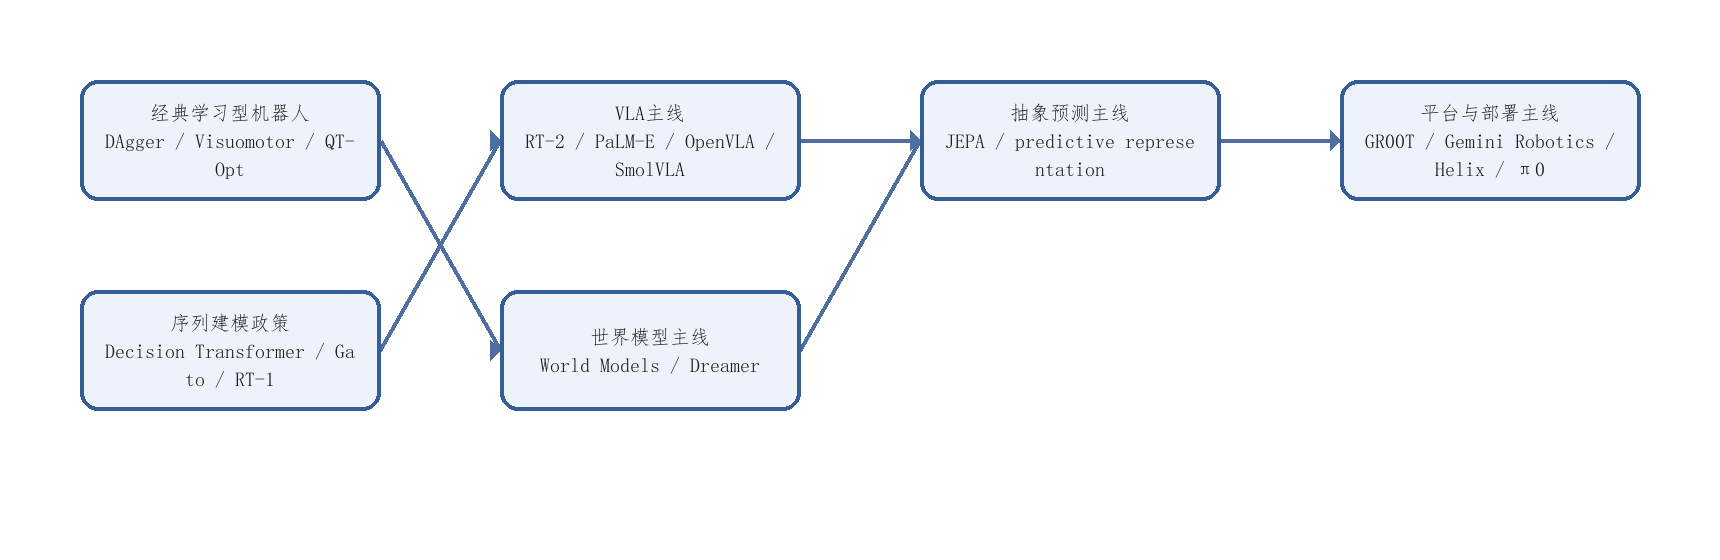
\includegraphics[width=0.9\textwidth,height=0.72\textheight,keepaspectratio]{figures/18-论文谱系时间线图.png}
\caption{18-论文谱系时间线图}
\label{fig:18-论文谱系时间线图}
\end{figure}

\section*{谱系维护补充}
\addcontentsline{toc}{chapter}{谱系维护补充}
\markboth{谱系维护补充}{谱系维护补充}

本章后续最值得固定成正式资产的，是完整论文谱系时间线与 \path{VLA / 世界模型 / 轻量部署} 三条谱系对照表。前者帮助读者追踪主线演化，后者帮助读者避免把不同目标函数、不同部署假设、不同研究对象误读成同一条线性升级路径。

这类补充之所以重要，是因为论文谱系章节的价值不在“列全”，而在“持续提供稳定比较框架”。

在当前版本中，\texttt{\detokenize{图 18-1 论文谱系时间线图}} 已承担主时间线职责；\texttt{\detokenize{表 18-1 论文谱系字段表}} 与 18-论文谱系时间线表 则共同承担结构化记录与时间轴维护职责。

\path{VLA / 世界模型 / 轻量部署} 三条主线之所以值得并行梳理，是因为它们分别对应“统一接口能力”“未来后果建模能力”与“真实部署约束吸收能力”三种不同的系统目标。把这些论文放回同一谱系里比较，可以减少“模型名字不同就像是不同代际”的错觉，也能帮助读者识别哪些工作只是改进单点性能，哪些工作真正推动了系统结构变化。

如果后续要做更严格的增量维护，本章建议优先同时配合两张结构化表来读：一张是字段表 18-论文谱系字段表，用于固定“怎么记录一篇论文”；另一张是 18-论文谱系时间线表，用于固定“怎么把论文放回年份与主线里”。前者解决记录口径，后者解决时间结构；两者合在一起，才能真正支撑后续季度增量更新。

为了维持这一章的长期可更新性，新增高价值论文更适合先沉淀为 \path{research/papers/} 下的论文卡，再回写正文判断。这样做的意义，不只是资料整理方便，更在于先把方法、实验边界、贡献与局限拆解清楚，再决定它应被放回哪条技术主线中。目前可直接复用的首批卡片包括：

\begin{enumerate}
\item RT-1 论文卡
\item RT-2 论文卡
\item PaLM-E 论文卡
\item OpenVLA 论文卡
\item SayCan 论文卡
\item Code as Policies 论文卡
\item DreamerV3 论文卡
\item Diffusion Policy 论文卡
\item V-JEPA 论文卡
\item GR00T N1 论文卡
\end{enumerate}

如果后续更新已经不再是“补一两篇论文”，而是需要批量判断整条路线的变化，则建议先读路线清单，再回到单篇卡：

\begin{enumerate}
\item VLA 论文清单
\item 世界模型论文清单
\item 规划与具身推理论文清单
\item 生成式动作与策略论文清单
\item 硬件、部署与系统工程论文清单
\item 仿真、评测与基础设施论文清单
\item 开源生态与工具链论文清单
\end{enumerate}

\section*{表 18-1 论文谱系字段表}
\addcontentsline{toc}{chapter}{表 18-1 论文谱系字段表}
\markboth{表 18-1 论文谱系字段表}{表 18-1 论文谱系字段表}

\begingroup
\small
\begin{xltabular}{\textwidth}{YYY}
\toprule
字段 & 含义 & 为什么必须记录 \\
\midrule
\endfirsthead
\toprule
字段 & 含义 & 为什么必须记录 \\
\midrule
\endhead
所属主线 & 该工作属于 VLA、world model、模仿学习、规划接口等哪条主线 & 防止新增论文变成新闻时间线 \\
输入输出接口 & 输入历史多长、是否含本体状态、输出单步动作还是 chunk、是否为技能接口 & 决定工作之间是否真的可比较 \\
数据来源 & 示教、遥操作、仿真、互联网视频、跨平台混合等 & 决定结论的适用边界 \\
训练范式 & 行为克隆、diffusion、flow matching、RL、混合式等 & 帮助识别能力来源 \\
泛化目标 & 新对象、新环境、新任务组合、跨本体等 & 防止把不同强度的泛化混为一谈 \\
部署假设 & 是否默认理想化本体、离线评测或真实闭环 & 判断离交付有多远 \\
开源程度 & 代码、权重、数据接口、评测脚本是否开放 & 评估其对社区扩散的影响 \\
未解决问题 & 当前仍留下的核心瓶颈 & 为后续版本跟踪留下接口 \\
\bottomrule
\end{xltabular}
\endgroup

\section*{表 18-2 论文谱系时间线表}
\addcontentsline{toc}{chapter}{表 18-2 论文谱系时间线表}
\markboth{表 18-2 论文谱系时间线表}{表 18-2 论文谱系时间线表}

\begingroup
\small
\begin{xltabular}{\textwidth}{YYYYYY}
\toprule
年份 & 代表工作 & 主线 & 所在层 & 在谱系中的角色 & 对应章节 \\
\midrule
\endfirsthead
\toprule
年份 & 代表工作 & 主线 & 所在层 & 在谱系中的角色 & 对应章节 \\
\midrule
\endhead
2022 & SayCan & 语言规划 & 规划层 & 把语言规划与技能可供性结合 & 12 \\
2022 & Code as Policies & 程序化规划 & 规划层 & 把语言输出约束到可执行程序接口 & 12 \\
2022 & RT-1 & VLA / 通用策略 & 模型层 & 早期机器人 Transformer 路线代表 & 11 \\
2023 & PaLM-E & embodied multimodal & 模型层 & 把多模态基础模型叙事推进到具身接口 & 11 / 21 \\
2023 & RT-2 & VLA / 通用策略 & 模型层 & 把互联网语义知识继续压向机器人动作接口 & 11 \\
2023 & Voyager & 记忆与长程代理 & 规划层 & 强调技能积累与外部记忆 & 12 \\
2024 & OpenVLA & 开源 VLA & 模型层 & 提供开源可复审的 VLA 对照点 & 11 \\
2025 & GR00T N1 & 平台型基础模型 & 平台层 & 将 humanoid、本体、仿真与基础模型组织到同一叙事 & 21 \\
\bottomrule
\end{xltabular}
\endgroup

这两张表分别解决“怎么记一篇论文”和“怎么把它放回主线时间结构”两个问题，是本章后续版本维护时比单纯补段落更重要的稳定资产。

% Generated from 19-开源生态、代码库与工具链.md; edit the LaTeX source after migration.

\part*{第十九部分 开源生态、代码库与工具链}
\addcontentsline{toc}{part}{第十九部分 开源生态、代码库与工具链}
\markboth{第十九部分 开源生态、代码库与工具链}{第十九部分 开源生态、代码库与工具链}

具身智能领域的开源生态与纯软件 AI 有一个明显不同：它不仅包含模型代码，还包含数据格式、机器人接口、仿真环境、评测协议和部署工具。也正因为如此，开源生态在机器人领域既是研究扩散器，也是能力过滤器。一个方向若没有开源支撑，研究社区很难充分比较；但即使开源存在，也不代表该路线足够接近真实部署。

更准确地说，具身开源生态不是一个平面的“代码仓库集合”，而是一套层层嵌套的基础设施：上游有视觉 backbone、自监督表征与通用训练框架；中游有机器人策略模型、数据格式、仿真与 benchmark；下游还有数据采集、日志回放、边缘推理、部署监控和 ROS/中间件接口。理解这个生态时，最重要的不是“哪个仓库最火”，而是它在这条链路上处于哪个位置，以及它暴露了多少真实系统假设。

\chapter*{91. 开源模型}
\addcontentsline{toc}{chapter}{91. 开源模型}
\markboth{91. 开源模型}{91. 开源模型}

\section*{91.1 机器人基础模型}
\addcontentsline{toc}{section}{91.1 机器人基础模型}


因此，阅读这类项目时最值得优先检查的通常是四件事：数据接口是否公开、动作表示是否明确、评测脚本是否可复现、部署约束是否被说明。只有这四项同时透明，基础模型才真正具备被社区继承和审查的价值。否则，它更像一个展示研究方向的样板，而不是一套可积累的公共资产。 把“机器人基础模型”作为开源生态中的一类对象单列出来，是因为它们往往不只是一个 checkpoint，而是一整套关于数据接口、动作表示、多任务条件化和评测方法的默认设定。对学习者而言，看这类项目时最重要的不是先问“参数有多大”，而是先问“它假设机器人问题该被怎样组织”。 但评价这类开源基础模型时，不能只看“是否开源了权重或代码”，还要看它是否把训练接口、动作表示、数据协议和评测脚本同时开放出来。对机器人来说，单独公开一个 checkpoint 的价值有限，因为真正决定复现与迁移成本的，往往是数据切片逻辑、动作 token 化方式、传感输入规范和与执行栈的绑定关系。也正因如此，能够把这些接口一并暴露出来的项目，往往比单点模型开源更有长期研究价值。

从学习路径上看，这类项目最适合承担“读懂问题设定”的功能，而不一定最适合直接变成你的第一套可部署系统。也就是说，它们往往更像研究接口样板，而不是现成产品模板。

OpenVLA 等项目的重要性，在于它们首次让研究者更系统地观察 VLA 路线的训练与部署接口，而不是只能依赖闭源演示理解其能力边界。\href{https://arxiv.org/abs/2406.09246}{OpenVLA}

我更建议把“机器人基础模型开源度”再拆成三层来看。第一层是论文级开放，只告诉你模型大致结构；第二层是代码/权重级开放，让你能真正复现实验；第三层是协议级开放，把数据 schema、动作表示、评测脚本、适配方法和部署入口一起公开。只有到第三层，项目才更接近可继承基础设施。像 \href{https://github.com/openvla/openvla}{OpenVLA GitHub} 这种同时公开模型、数据接口、微调与服务化入口的项目，和只给 checkpoint 或演示脚本的项目，研究价值并不在同一个数量级上。

\section*{91.2 policy 学习模型}
\addcontentsline{toc}{section}{91.2 policy 学习模型}


policy 学习模型这一类开源项目的真正价值，在于它们把机器人动作生成问题变成可直接替换、比较和复用的研究接口。不同仓库虽然名字各异，但常常围绕同几类分歧展开：动作是回归、扩散还是 token；输入窗口多长；是否支持多任务；是否显式建模恢复或闭环重规划。 这一类开源 policy 项目的真正意义，是把机器人动作学习从“彼此难以比较的私有实验”逐步推进成“至少在接口层可互译的研究对象”。它们提供的不只是算法实现，更是一套默认问题设定：观测窗口如何构造、动作是逐步输出还是 chunk 输出、损失函数如何兼顾平滑性与目标完成、评测时是否允许重规划。换句话说，policy 开源生态实际上在不断塑造研究共同体默认承认什么叫“可比较的动作学习结果”。

对报告维护者而言，这意味着后续每看到一个新 policy 仓库，都应先判断它是在重写哪一层默认设定，而不是只记录“又多了一个新模型名”。只要把这一习惯固定下来，第 19 章就不会沦为仓库名单。

这些工作为更通用的策略学习提供了基线，使动作生成、轨迹建模和条件化策略学习得以进入更统一的比较框架。代表性论文可参见 \href{https://arxiv.org/abs/2303.04137}{Diffusion Policy：扩散式机器人策略}、\href{https://arxiv.org/abs/2106.01345}{Decision Transformer：序列化决策} 与 \href{https://arxiv.org/abs/2304.13705}{ACT：动作块 Transformer}。

如果把这一类开源 policy 按“动作是怎样被组织出来的”来分层，至少可以得到四类主流写法。第一类是\texttt{\detokenize{自回归序列策略}}，其典型形式更接近

\begin{equation*}
p(a_t \mid o_{\le t}, a_{<t}, g)
\end{equation*}

即把决策写成条件序列建模问题，\href{https://arxiv.org/abs/2106.01345}{Decision Transformer：序列化决策模型} 是这一思想在决策领域的经典入口。第二类是\texttt{\detokenize{动作块策略}}，直接预测未来 \(H\) 步动作片段，

\begin{equation*}
p(a_{t:t+H-1} \mid o_{\le t}, g)
\end{equation*}

这样做的好处是减少逐步解码抖动，\href{https://arxiv.org/abs/2304.13705}{ACT：动作块 Transformer} 就把“动作块”明确写成策略接口。第三类是\texttt{\detokenize{扩散式动作策略}}，以迭代去噪方式生成动作序列，\href{https://arxiv.org/abs/2303.04137}{Diffusion Policy：扩散式机器人策略} 代表了这种路线，其优势在于对多峰动作分布的刻画能力更强。第四类则是\texttt{\detokenize{通用策略底座 + 跨本体数据协议}}路线，例如 \href{https://arxiv.org/abs/2405.12213}{Octo：开源通用机器人策略}、\href{https://arxiv.org/abs/2406.09246}{OpenVLA：开放视觉-语言-动作模型} 与 \href{https://arxiv.org/abs/2310.08864}{Open X-Embodiment：跨本体机器人数据开放协议} 所共同推动的方向：不再只优化单一本体上的策略拟合，而是把动作接口、数据模式与迁移方式一起做成生态对象。

因此，读一个开源策略项目时，至少应先看四个维度。第一是\texttt{\detokenize{动作表示}}：到底输出单步连续动作、动作块、离散动作记号还是技能索引。第二是\texttt{\detokenize{时间抽象}}：它是在毫秒级控制上出动作，还是在较低频率上出未来一段动作计划。第三是\texttt{\detokenize{跨本体适配方式}}：它假设所有机器人共享同一动作语义，还是允许通过适配器、归一化和数据模式映射来组织差异。第四是\texttt{\detokenize{运行时接口}}：模型训练出来之后，是只停留在笔记本实验或离线展开脚本，还是已经暴露推理服务、机器人适配、日志和回放接口。只要这四维被看清，一个策略仓库的研究位置就会比“代码托管平台热度高不高”更明确。

从这个角度看，policy 开源项目还可以进一步分成三类资产。\texttt{\detokenize{研究样本}}主要公开论文对应实现，用于说明方法是否成立；\texttt{\detokenize{系统样本}}开始把数据处理、评测和部署入口一起暴露出来，用于说明方法如何接进真实软件栈；\texttt{\detokenize{基础设施样本}}则进一步把数据 schema、训练脚本、机器人适配、回放和运行时服务都稳定公开，使后来者可以在其上持续叠加。像 \href{https://github.com/openvla/openvla}{OpenVLA GitHub} 与 \href{https://github.com/huggingface/lerobot}{LeRobot GitHub} 之所以值得长期跟踪，正是因为它们开始显式提供第二类甚至向第三类过渡的资产，而不只是“模型权重下载入口”。

同样重要的是，要把失败模式一起写进阅读框架。当前开源 policy 最常见的四类脆弱点是：第一，\texttt{\detokenize{恢复盲区}}，即模型擅长主路径模仿，却缺少失败后回退与二次尝试能力；第二，\texttt{\detokenize{动作接口错配}}，即离线动作格式与真实控制器消费接口不一致；第三，\texttt{\detokenize{时延敏感性}}，即模型在离线 rollout 中表现良好，但在边缘设备或网络链路上推理抖动明显；第四，\texttt{\detokenize{跨本体幻觉}}，即表面上支持多机器人训练，实际上控制频率、夹具和示教语义并未真正对齐。只要这些问题没有被公开处理，再漂亮的开源 policy 也更接近“研究现象样本”而不是“可继承工程资产”。

对后续版本维护而言，这一节最值得固定成纪律的不是项目名单，而是一条阅读顺序：

\begin{enumerate}
\item 先看数据协议：这个 policy 默认读取什么 schema、什么时间切片、什么动作语义。
\item 再看动作表示：它输出单步、chunk、token 还是技能。
\item 再看评测协议：它的 benchmark 到底奖励主路径命中、恢复能力还是长时稳定性。
\item 最后看运行时接口：它是否真正暴露服务化、日志、适配和回退入口。
\end{enumerate}

只要沿着这条顺序去读，新项目就更不容易把我们重新拉回“仓库很热所以路线很重要”的浅层判断。

\section*{91.3 多模态与世界模型相关开源项目}
\addcontentsline{toc}{section}{91.3 多模态与世界模型相关开源项目}


这一类项目的真正价值，在于它们虽然不一定直接输出机器人动作，却经常决定机器人系统能带着什么样的表征先验进入训练。视觉 backbone、自监督表示学习库、视频预测框架和多模态训练基座，往往在机器人专用仓库之前就已经改写了输入表示、时间建模方式和跨模态对齐接口。若只盯着最下游 policy 仓库，读者很容易错过这些更高杠杆的变化。

因此，更稳妥的阅读方法不是把它们视为“外围材料”，而是把它们放进同一条具身软件栈里理解：上游项目决定先验与表示，中游项目决定动作建模接口，下游项目决定评测与部署可行性。只有建立这种分层视角，开源生态才会从零散仓库收藏夹，变成可复用的研究地图。 这类项目的重要性，在于它们虽然不一定直接输出机器人动作，却决定了机器人上游表征、视频预测、抽象状态建模和多模态对齐能力的边界。很多机器人基础模型表面属于“机器人代码库”，底层却大量复用这些更通用的多模态资产。 这类项目常常不是直接面向机器人部署，却对后续具身路线产生上游决定性影响。很多机器人基础模型表面上是“机器人论文”，底层却大量借用了视觉 backbone、视频预测模型、自监督表征学习库和通用多模态训练框架。因而研究者若只跟踪机器人专属仓库，很容易错过真正改变接口能力的上游变化。理解开源生态时，必须把“机器人项目”与“机器人所依赖的通用表征资产”放在同一张图里。

世界模型、感知 backbone、自监督表示学习和视频预测的开源实现，则为后续机器人基础模型提供了大量上游组件。很多“机器人模型”真正依赖的，其实是这些更一般的开源表示学习资产。

这提醒我们在阅读机器人开源项目时，不应只盯着最下游 policy 仓库。很多决定系统上限的变化，其实先发生在上游视觉、自监督、多模态和视频建模资产中，而机器人仓库只是把这些能力重新绑到动作接口上。

\section*{91.4 轻量化与端侧路线的开源意义}
\addcontentsline{toc}{section}{91.4 轻量化与端侧路线的开源意义}


轻量化开源路线还有一个经常被忽视的价值：它更早暴露真实部署约束。大模型演示往往默认充足算力、干净网络和高成本硬件，而轻量化项目会迫使社区正视模型尺寸、推理时延、内存占用、热设计功耗和设备成本这些不浪漫却决定落地成败的问题。因此，这类路线虽然在“能力想象空间”上不如巨型模型耀眼，但在“什么东西真正能在机器人上跑起来”这件事上，往往更接近现实。

SmolVLA、LeRobot 等路线之所以值得跟踪，不只是因为它们“能跑在更小机器上”，而是因为它们把低成本复现、社区参与和端侧约束一起变成研究目标。这与只发布一个大模型 checkpoint 的意义完全不同。\href{https://arxiv.org/abs/2506.01844}{SmolVLA}、\href{https://arxiv.org/abs/2602.22818}{LeRobot}

这类路线还有一个研究方法上的额外价值：它们迫使社区把“真实机器人算力预算”重新写回实验设计。过去很多研究默认离线训练与在线推理的资源约束完全不同，因此模型结构可以任意膨胀；而轻量化路线会逼迫研究者重新回答几个不那么浪漫但极其关键的问题：

\begin{enumerate}
\item 模型能否在板载设备稳定运行。
\item 量化、蒸馏与裁剪是否会破坏动作稳定性。
\item 端侧延迟抖动会不会直接影响闭环控制。
\item 小模型是否仍然保留足够的恢复与重试能力。
\end{enumerate}

也因此，轻量化开源项目的价值常常不在于“指标最强”，而在于它们更早暴露出哪些能力是真正可以被部署继承的，哪些能力只是靠高算力实验环境暂时堆出来的。

这一层近两年最值得重视的变化，是轻量化项目不再只发布“压缩版模型”，而开始把低门槛硬件、统一数据格式和最小复现实验一起交给社区。\href{https://github.com/huggingface/lerobot}{LeRobot} 明确把真实机器人训练、评测、遥操作、低成本机械臂与硬件无关接口放进同一项目叙事；\href{https://arxiv.org/abs/2506.01844}{SmolVLA} 则把“小模型也要保留真实机器人可用性”作为正式研究目标。这说明端侧开源路线的价值，已经从“给弱设备一个替代品”升级成“把真实部署约束重新写回研究默认设定”。

\chapter*{92. 开源数据集与 benchmark}
\addcontentsline{toc}{chapter}{92. 开源数据集与 benchmark}
\markboth{92. 开源数据集与 benchmark}{92. 开源数据集与 benchmark}

\section*{92.1 操作数据集}
\addcontentsline{toc}{section}{92.1 操作数据集}


操作数据集最容易被误读的地方，是外界常常只盯着轨迹条数或任务数量，却忽略了协议层质量。对具身模型而言，更关键的问题往往是：动作空间是否一致，传感器与控制时间轴是否对齐，失败样本是否被完整保留，episode 边界如何定义，任务标签是否稳定，元数据能否支持跨任务重采样。这些看起来“工程化”的细节，往往比样本总量更决定可学性。

也因此，一个真正高价值的操作数据集，通常不只是数据文件本身，还包括清洗脚本、对齐规则、重采样工具、成功判定协议和版本化维护方法。若这些内容缺失，再大的数据池也可能很难转化成稳定的监督资源。 操作数据集之所以要单列，是因为它们定义了机器人“如何被看作一个训练样本生成器”。一个好的操作数据集不仅要有成功轨迹，还要有清晰动作接口、时间同步、失败样本、任务标签和足够可解释的元数据。 对操作数据集的判断也不能停留在“规模大不大”。真正关键的是它是否清楚定义了动作接口、对齐了传感与控制时间轴、覆盖了多少失败样本，以及任务成功究竟是以什么标准标注。一个看起来规模不小的数据集，如果动作协议混乱、示教质量不均或失败片段被大量过滤掉，最后很可能更适合做演示型模仿，而不适合做稳健闭环学习。

Open X-Embodiment 的重要性在于它尝试把跨平台机器人数据组织成可比较接口，这是机器人数据工程走向基础模型的关键一步，相关论文可参见 \href{https://arxiv.org/abs/2310.08864}{《Open X-Embodiment》}。

\section*{92.2 导航与移动数据集}
\addcontentsline{toc}{section}{92.2 导航与移动数据集}


导航与移动数据集的价值，在于它们更早把长期任务、地图记忆、重定位和场景级评测问题组织成了较成熟的 benchmark 传统。对具身学习者来说，这类传统很有借鉴意义，因为它说明：很多看似“新”的长时程问题，其实早已在移动机器人与 embodied AI 里被系统化处理过。 导航数据集和 benchmark 的长期价值，在于它们更早积累了“场景级结构化评测”传统。这类传统对具身智能很重要，因为它提醒我们：真正困难的问题往往不在单步感知，而在长时程任务中如何处理记忆、重定位、地图误差和恢复。也正因如此，导航生态里那些关于 episode 定义、重置条件、成功半径和探索预算的设计经验，后来都对更广义 embodied AI 问题产生了迁移价值。

导航和具身智能研究社区长期积累了大量场景级数据集与评测基准，为长时程任务、场景记忆和环境交互研究提供了可复用基础。Habitat 等环境也让“导航评测并不是单个数据集，而是一套可反复实例化的实验接口”这一点更清楚，相关资料可参见 \href{https://aihabitat.org/}{Habitat 项目主页}。

\section*{92.3 多机器人 / 多模态数据集}
\addcontentsline{toc}{section}{92.3 多机器人 / 多模态数据集}


多机器人 / 多模态数据集的真正价值，不只是“样本量更大”，而是它们尝试统一观测、动作、时间戳、元数据与任务描述接口，使不同本体、不同传感器组合、不同采集流程之间第一次出现最基本的互操作可能。Open X-Embodiment 的启发也在这里：如果行业长期停留在各家自定义数据模式、各家自定义 episode 格式，就很难形成可持续的跨平台学习生态，相关论文可参见 \href{https://arxiv.org/abs/2310.08864}{《Open X-Embodiment》}。

但把多源数据拼在一起，并不自动等于“可以直接联合训练”。不同本体的自由度、夹具、控制频率、接触边界和示教质量差异极大；不同模态之间还存在同步误差、缺失机制与噪声模型差异。因此真正有价值的数据集，往往还伴随对齐层、字段标准化、重采样策略与质量标签，否则规模优势很容易被分布错位抵消。

对具身智能而言，这类数据集最值得关注的，不只是它们是否提升了单次训练结果，而是它们是否在事实上推动了跨本体接口标准的形成。谁能把 episode schema、动作语义、传感器同步与评测协议稳定下来，谁就更可能影响后续生态，而不仅仅是贡献一个更大的数据池。 这类数据集最值得追问的问题，不是“规模大不大”，而是“不同平台之间到底对齐了什么”。如果只是把日志放进同一存储格式，但动作含义、传感器节奏和任务结构并未真正对齐，那么所谓统一数据集对基础模型训练的帮助也会受到很大限制。 这类数据集往往最容易在论文摘要中显得“通用”，却也最容易在细节上失去可比性。不同机器人平台的动作空间、控制频率、相机布局、示教方式和任务拆分方式一旦差异过大，所谓“统一数据集”就可能只是在存储层被拼接到了一起，而没有在语义层和控制层真正对齐。因此，评估这类开源资源时，最需要追问的往往不是规模，而是它到底统一了什么、又刻意保留了哪些不可统一差异。

这类数据集对通用性很重要，但也更容易隐藏平台差异和对齐困难，因此解读时必须警惕“看起来规模很大，但动作接口并不一致”的问题。

\section*{92.4 benchmark 为何也是“方法偏置”}
\addcontentsline{toc}{section}{92.4 benchmark 为何也是“方法偏置”}


从研究方法论上看，benchmark 本身就是一种隐形论文作者。它通过奖励什么、忽略什么来持续筛选研究路线。若 benchmark 主要奖励单次成功率，研究者就会倾向于优化静态命中；若它强调重试、恢复、鲁棒性和分布外扰动，路线就会更靠近真实部署。因而阅读开源 benchmark 时，不能把它当作中立舞台，而应把它视为一组被编码进评测协议里的价值判断。

评测基准并不是中性裁判。一个基准强调单步成功率，和一个基准强调长时程恢复能力，最终会把研究路线推向完全不同方向。因此，评估开源数据与评测基准时，必须同时问：它定义了什么问题，又把什么问题排除在外。

对学习者来说，一个很实用的习惯是：每看到一个 benchmark，就先写下它主要奖励什么、弱化什么、默认了哪些本体与场景假设。这样后续再看模型排名时，就不容易把“在这个 benchmark 下最强”误读成“在现实系统里最强”。

这一点与 14-评测指标分层表 可以互相配合。前者帮助判断 benchmark 奖励什么，后者帮助判断这些奖励是否足以支撑真实部署判断。

如果把这层理解再向前推进一步，那么 benchmark 实际上还承担着“分配研究注意力”的经济功能。社区时间、算力和复现资源都是有限的，哪些任务更容易被 benchmark 化，哪些指标更容易被排行榜化，就更容易持续吸收研究投入。因此，benchmark 的设计不是中性的学术细节，而是决定哪些方向会越来越热、哪些困难会被长期低估的结构力量。

这也解释了为什么本章要把 benchmark 和工具链放在一起讨论。一个 benchmark 若没有稳定脚本、公开环境、统一日志格式和易复用评测接口，它即使概念很好，也很难形成真正社区牵引力；反过来，一个工具链若天然支持某类评测，就会反向推动这类评测逐渐变成事实标准。理解这层互动后，开源生态才不再只是“仓库的集合”，而会变成“研究范式如何自我放大的机制图”。

\chapter*{93. 代码生态与工程工具链}
\addcontentsline{toc}{chapter}{93. 代码生态与工程工具链}
\markboth{93. 代码生态与工程工具链}{93. 代码生态与工程工具链}

\section*{93.1 训练框架}
\addcontentsline{toc}{section}{93.1 训练框架}


训练框架不只是“把模型跑起来的代码壳”，而是把数据切片、批处理、分布式训练、日志追踪、检查点管理和评测调用串成稳定工作流的中间基础设施。对具身系统而言，这一点尤其重要，因为训练对象往往不是单一张量，而是图像、状态、动作、语言、时间戳和任务上下文共同组成的多模态序列。

一个最小训练框架通常至少要回答四个问题：怎么读数据、怎么切序列、怎么组织损失、怎么在训练后调用评测。其极简骨架可以写成：

\begin{lstlisting}[language=python]
dataset = load_robot_dataset(config)
batch = sample_multimodal_batch(dataset)
loss = model.compute_loss(batch)
loss.backward()
optimizer.step()
evaluator.maybe_run(model)
\end{lstlisting}

训练框架的成熟度还决定了社区能否把单次论文结果沉淀成持续可迭代工作流。一个真正有价值的训练框架，通常不只是“能跑通作者方法”，而是能支持数据版本化、分布式训练、日志追踪、失败复现实验和多模型接口替换。也就是说，训练框架决定的不只是实验效率，更是一个方向能否从论文代码成长为长期研究基础设施。

从通用深度学习训练框架到专门的机器人策略训练库，当前生态正在逐渐把多模态训练、动作 token 化、数据切片与分布式训练组织成更标准的工作流。

\section*{93.2 仿真与评测工具}
\addcontentsline{toc}{section}{93.2 仿真与评测工具}


这类工具的公共价值常常高于单个模型仓库，因为它们决定了不同路线能否被放到同一坐标系里比较。一个社区如果只有模型、没有共同环境脚本与评测协议，结果往往是“每篇论文都自带一套世界”。从长期知识积累角度看，仿真与评测工具链越公开、越标准化，整个领域越容易形成真正可继承的结论，而不是短期演示繁荣。 仿真与评测工具之所以应该单独看待，是因为它们承担的不是同一职责。仿真工具负责生成可交互环境、可控扰动和可重复试验；评测工具则负责把任务、度量、日志与结果统计固定成协议。前者回答“能不能在某个世界里试”，后者回答“试完以后怎么比较”。

从工具链分工看，这一层至少包括：

\begin{enumerate}
\item 环境实例化与 reset。
\item 传感器模拟与状态读取。
\item 任务脚本与扰动注入。
\item 指标统计、回放与可视化分析。
\end{enumerate}

Isaac、Habitat、MuJoCo、ROS/Gazebo 等平台构成了机器人研究最重要的工具链底座。问题不在“哪个最好”，而在不同工具链分别服务于什么能力边界；相关入口可参见 \href{https://developer.nvidia.com/isaac/sim}{Isaac Sim}、\href{https://aihabitat.org/}{Habitat}、\href{https://mujoco.org/}{MuJoCo} 与 \href{https://gazebosim.org/home}{Gazebo}。

如果再往前走一步，我会建议把“仿真工具”与“仿真训练框架”分开看。前者更接近物理与渲染底座，后者则决定如何在这些底座上批量生成任务、并行训练与做回归评测。\href{https://github.com/isaac-sim/IsaacLab}{Isaac Lab} 的价值，就不只是另一个仿真器，而是把“大规模并行机器人学习”组织成了更可重用的训练框架；\href{https://aihabitat.org/}{Habitat} 则更长期地承担了 embodied AI 环境、场景任务与评测接口的统一入口。对学习者而言，这种区分很重要，因为很多时候真正缺的不是“再多一个物理引擎”，而是“把训练和评测规模化组织起来的脚手架”。

\section*{93.3 数据采集与标注工具}
\addcontentsline{toc}{section}{93.3 数据采集与标注工具}


对具身智能来说，数据工具链的重要性甚至接近模型本身，因为许多性能差异最终都来自数据采集协议、时间同步质量、失败片段保留率和元数据完整性差异。一个看似普通的录制与回放工具，只要能稳定记录语言、视频、机器人状态、动作和异常标签之间的时序关系，就足以显著改变后续训练闭环质量。这也是为什么很多真正有长期壁垒的团队，都会把数据工具链视为核心资产而不是附属脚本。 数据采集与标注工具的核心，不只是“把数据录下来”，而是把具身交互过程变成可回流训练的结构化资产。一个完整链路通常包括：遥操作或自动脚本采集、多模态时间同步、失败片段筛选、元数据记录、回放验证和标准格式导出。

其最小工作流可以写成：

\begin{lstlisting}[language=python]
episode = recorder.start()
while task_active:
    recorder.log(obs, action, state, language, timestamp)
episode = recorder.stop()
dataset_writer.export(episode, schema="robot_standard")
\end{lstlisting}

对机器人社区来说，这类工具链的战略地位常常被低估。因为很多团队真正缺的不是再多一个 policy 网络，而是如何稳定录制遥操作轨迹、保证多模态时间同步、把失败片段筛出来、把现场日志组织成可回流训练样本。谁能把这条链路工具化，谁就更容易把零散实验积累成持续闭环。因此，数据工具链往往比单个模型仓库更接近真实护城河的雏形。

遥操作记录、时间同步、日志回放和失败样本筛选工具，是学习型机器人闭环能否形成的关键中间层。

\section*{93.4 部署与推理工具}
\addcontentsline{toc}{section}{93.4 部署与推理工具}


部署与推理工具在具身智能里的特殊性在于，它们不是单纯把模型“导出一下”就结束，而是要回答四个系统问题：模型怎样被压缩或蒸馏；推理怎样与中间件和控制器对时；日志怎样回放和归因；失败时怎样切换到本地回退控制或人工接管。因此，这一层工具链的价值，往往比论文中的单次推理速度数字更大。

对学习者而言，部署工具最有用的不是“能不能一键跑”，而是它是否让你看见真实系统中那些论文常省略的接口：消息频率、缓存策略、状态同步、监控报警、回退控制、模型版本切换和现场日志。谁能把这些接口暴露出来，谁就更接近真实工程。 部署与推理工具关注的，不再是“模型训练得好不好”，而是“模型能否在真实机器人运行栈中稳定存在”。这一层通常包括模型压缩、运行时封装、设备侧调度、异常监控、回放与告警。它的输入是训练好的模型，输出则是一个能在具体硬件、通信链路和时延预算下工作的服务。

一个极简部署链路可以抽象为：

\begin{lstlisting}[language=python]
runtime = load_runtime(target_device="edge_gpu")
model = runtime.optimize_and_load(checkpoint)
while robot_is_running:
    obs = middleware.read()
    action = model.infer(obs)
    middleware.write(action)
\end{lstlisting}

这一层工具之所以重要，是因为它决定了“论文能力”能否跨过最后一公里。模型压缩、端侧 runtime、实时调度、健康监测、回放与告警机制，看起来不像核心算法，却直接决定一个系统能否在现场长时间稳定运行。很多开源生态之所以长期停留在研究演示层，并不是缺少更强模型，而是缺少把模型嵌入真实机器人运行栈的部署级公共资产。

边缘推理、模型压缩、实时调度和日志监控工具，会越来越成为开源生态价值的重要组成，而不只是“论文附带代码”。

真正成熟的具身开源生态，最终不会只由训练脚本和 checkpoint 组成，而会越来越多地包含运行时、监控、回放、压缩和部署接口。这也是判断一个项目是否开始接近“公共基础设施”而不只是“研究仓库”的一个重要信号。

这一层之所以值得被单独强调，还因为它是许多研究路线最终失真最严重的地方。论文里经常默认“模型可推理”就接近“系统可运行”，但现实部署要额外处理 runtime 兼容、消息同步、监控指标、模型回滚、异常注入、边缘设备健康状态和任务中断恢复。谁把这些接口公开出来，谁就更接近真正可继承的工程资产；谁始终停留在离线推理脚本层，谁的开源价值就更偏向研究启发，而非部署基础设施。

对长期学习者而言，这里还有一个很实用的判断：若某个项目只公开训练代码而几乎没有回放、监控、部署和回退相关资产，那么阅读它时就应主动把它定位成“算法样本”；若它连运行时、日志、监控和版本切换接口都开始显式出现，就值得把它上调为“系统样本”甚至“基础设施样本”。这类分层判断，有助于避免把所有热门仓库都误看成同一种资产。

从这个标准出发，当前最值得重视的开源变化，是越来越多项目开始公开“训练之后怎么办”。例如 \href{https://github.com/openvla/openvla}{OpenVLA GitHub} 已经把推理服务、机器人适配和后续微调入口显式暴露出来；\href{https://github.com/huggingface/lerobot}{LeRobot} 则把数据采集、真实机器人评测、模型训练和部署链路组织成一套更完整的研究工作台。它们未必已经解决了全部部署问题，但至少把社区最容易缺失的那一层接口第一次变得足够可见了。

\section*{93.5 一个更实用的工具链分层法}
\addcontentsline{toc}{section}{93.5 一个更实用的工具链分层法}


如果把开源工具链按“学习者真正会怎么用”来分层，一个更实用的四层划分是：

\begin{enumerate}
\item 读接口层：看数据格式、输入输出张量、动作表示和任务脚本。
\item 复现实验层：能否在公开环境里复现实验、回放结果和评测流程。
\item 改任务层：能否替换对象、场景或本体，而不是只能按 demo 原样复刻。
\item 接系统层：能否与 ROS、仿真器、边缘推理和日志系统连起来。
\end{enumerate}

这套分层法的好处是，它能帮助你快速判断一个仓库适合拿来做什么。很多热门项目在第一层和第二层很强，却完全不适合直接进入第四层；反过来，一些工程仓库论文感不强，却对第四层价值很大。这样理解后，就不容易把“研究可见性”误判为“工程可交付性”。

对学习者而言，更有用的不是按“论文方向”记工具，而是按以下四层记：

\begin{enumerate}
\item 数据层：采集、清洗、回放、格式标准化。
\item 模型层：感知 backbone、policy、VLA、world model。
\item 环境层：仿真、benchmark、评测脚本。
\item 部署层：ROS/中间件、端侧推理、日志与监控。
\end{enumerate}

只有把工具放回这四层，才能真正理解一个项目缺的到底是“模型”还是“整条链路中的某一段”。

下面给出一个极简训练工具链伪代码，说明开源生态在现实中如何串起来：

\begin{lstlisting}[language=python]
dataset = load_robot_dataset("openx_or_local_logs")
batch = slice_multimodal_sequences(dataset)
features = vision_encoder(batch["images"])
actions = policy.train_step(features, batch["states"], batch["actions"], batch["language"])
evaluator.run(policy, benchmark="sim_or_real")
\end{lstlisting}

真正重要的，不是这几行代码本身，而是它暴露出具身开源生态的真实耦合方式：数据格式、切片逻辑、编码器、策略、评测脚本必须能够接在一起，生态才会产生复用价值。

把工具链按这四层来记，还有一个额外好处：它能帮助研究者迅速识别“当前卡点究竟在哪一层”。很多时候问题并不是模型不够强，而是数据层没有时间同步、环境层没有可比评测、部署层没有稳定 runtime。只要这一判断被做清楚，后续补工作就不会总是条件反射地继续换模型。

如果进一步把这四层写成最小研究工作流，那么一个成熟的开源学习路径通常是：

\begin{lstlisting}
1. 先读数据层：确认 schema、时间同步、动作接口和成功判定。
2. 再读模型层：确认输入输出、训练目标和动作表示。
3. 再读环境层：确认 benchmark 奖励什么、忽略什么。
4. 最后读部署层：确认哪些能力真正能进入运行栈。
\end{lstlisting}

这一路径的价值在于，它迫使学习者先搞清系统接口，再看模型亮点，而不是一上来就被网络结构和演示视频牵着走。对本报告后续维护来说，这也是最适合作为新增开源项目时的标准阅读顺序。

\chapter*{94. 开源与产业闭源路线的关系}
\addcontentsline{toc}{chapter}{94. 开源与产业闭源路线的关系}
\markboth{94. 开源与产业闭源路线的关系}{94. 开源与产业闭源路线的关系}

\section*{94.1 开源如何推动研究扩散}
\addcontentsline{toc}{section}{94.1 开源如何推动研究扩散}


从机制上看，开源推动研究扩散，至少依赖三条链路：接口公开、实验可复现、社区可接力。接口公开让别人知道一个方法到底依赖了什么输入输出；实验可复现让后续研究不必从零搭私有栈；社区可接力则让数据格式、评测脚本和工具插件围绕同一接口逐步积累。

若把这一过程写得更抽象一些，可以理解为：

\begingroup
\scriptsize
\begin{equation*}
\text{Open Source} \rightarrow \text{Shared Interface} \rightarrow \text{Reproduction} \rightarrow \text{Iteration}
\end{equation*}
\endgroup

更具体地说，开源推动扩散的机制主要有三种：第一，降低复现实验的进入门槛，让更多团队可以在同一接口上比较方法；第二，暴露隐含假设，使社区能够识别某条路线到底依赖了哪些数据协议、硬件先验和训练技巧；第三，为后续工作提供可继承起点，而不是每篇论文都从零搭建私有栈。对具身领域这种链路极长的方向而言，这三点尤其重要。

这也是为什么在具身领域里，“接口是否公开”有时比“指标是否领先一点”更重要。前者决定别人能否接着做、能否在同一协议下复审结论；后者若缺乏可复现接口，往往只会形成一轮新的演示消费，而不会转化为公共研究资产。

开源让模型接口、数据协议和 benchmark 比较更透明，也让研究者更容易发现某条路线真正依赖的假设。

更进一步说，开源最稀缺的贡献往往不是把代码“放出来”本身，而是把一条路线压缩成别人可以继承的公共结构。一个真正高价值的开源项目，至少会让后来者少踩三类坑：输入输出接口如何定义、训练与评测协议如何组织、系统失败后如何定位问题。只要这三层结构被公开，后来团队即使不完全沿用原实现，也更容易在同一问题空间内继续推进。

这也是为什么有些项目虽然参数规模不大、分数也未必第一，却能长期影响社区主线。它们留下的不是某个时点的最好结果，而是一个可被复用的问题框架。对研究型报告而言，这种框架价值往往比一次性的性能领先更值得高权重记录。

\section*{94.2 闭源如何形成护城河}
\addcontentsline{toc}{section}{94.2 闭源如何形成护城河}


闭源路线形成护城河，通常也不是因为“把模型文件藏起来”这么简单，而是因为它把多个难复制环节耦合在一起：真实数据采集网络、本体与软件协同设计、现场运维、故障回放资产、客户场景适配和供应链经验。也就是说，闭源优势往往是系统级复合优势，而不是单点算法秘密。

若把这种壁垒拆开，可以粗分为：

\begin{enumerate}
\item 数据壁垒：长期现场日志、失败样本和高质量示教。
\item 系统壁垒：硬件、控制、感知、调度与安全机制的耦合优化。
\item 交付壁垒：部署流程、运维网络、客户定制与迭代闭环。
\end{enumerate}

但闭源形成护城河的方式，也远比“把模型藏起来”复杂。真正难复制的，通常不是论文里那段核心网络，而是长时间积累的现场数据、故障回放资产、标注与回流流程、供应链 know-how、客户场景适配经验和运维网络。也正因为如此，很多企业即使在论文发表和公开视频上显得并不神秘，外部团队也很难短期追平其真实交付能力。

因此，理解闭源壁垒时最容易犯的错，是把它缩减成“他们肯定藏了更强的模型”。很多时候，真正难复制的是成百上千次现场失败如何被记录、谁来处理接管、哪些版本能安全回滚、以及不同客户场景是如何被逐步模板化的。这些资产哪怕论文里一句没写，也可能比单个模型结构更决定企业位置。

闭源企业真正的护城河往往不在论文文本，而在真实数据规模、本体耦合、系统集成经验和部署基础设施。

如果把闭源壁垒再抽象一步，可以把它理解为：

\begingroup
\scriptsize
\begin{equation*}
\text{Moat}_{closed} \approx \text{data} + \text{deployment} + \text{ops} + \text{integration}
\end{equation*}
\endgroup

这当然不是严格经济模型，但它提醒我们：闭源护城河通常是多种难复制资产的和，而不是单一模型权重文件。尤其在具身行业里，部署网络和异常恢复组织能力往往比“再多一个点的 benchmark 提升”更决定长期壁垒。

也因此，后续在企业专题里遇到“闭源很神秘”的说法时，更稳妥的做法不是猜它藏了什么，而是去追问它具体控制了哪一类复合资产：现场数据回流、硬件调参经验、版本回归体系、供应链协同，还是客户工作流嵌入能力。只要把资产类型拆开，闭源路线的真实位置通常会比宣传口径清楚得多。

\section*{94.3 对学习者与研究者的启发}
\addcontentsline{toc}{section}{94.3 对学习者与研究者的启发}


对学习者而言，更实用的策略通常不是在开源与闭源之间选边站，而是把二者当作不同类型的证据源。开源更适合理解结构、接口和可复现实验边界；闭源更适合理解哪些能力已经值得真实场景高成本投入。把这两类信号并读，往往比只追某一边更接近行业真实。

对研究者而言，一个同样重要的启发是：不要只问“有没有更强模型”，还要问“这条路线是否在开源生态中留下了可继承的接口资产”。后者往往比一次性的分数提升更能决定一个方向会不会变成长期主线。 因此，对个人研究者最稳健的策略不是在“开源信仰”和“闭源崇拜”之间选边，而是把两者当作不同性质的证据源。开源更适合理解结构、接口与可复现实验边界；闭源更适合理解什么能力在真实商业环境里被证明值得高成本投入。把这两类信号并读，往往比单独追任何一边更接近行业真实。

对个人研究者而言，最有效的策略通常不是执着区分“只看开源”或“只看闭源”，而是利用开源理解方法结构，再通过闭源路线检验哪些部分已经接近真实产业能力。

换句话说，开源更像显微镜，闭源更像压力测试。前者帮助我们看清方法细节、接口假设和复现路径，后者帮助我们判断哪些能力已经值得被高成本真实场景反复验证。把两者配合使用，才更接近具身行业的真实信息结构。

对学习者更实用的一条方法论是，把开源项目当成“接口教科书”，把闭源路线当成“价值筛子”。前者帮助理解系统通常如何组织，哪些环节容易暴露问题，哪些数据格式和评测协议已经成为事实标准；后者则帮助判断，行业究竟愿意为哪些能力支付真实金钱、真实运维成本和真实责任成本。两者合起来，才能避免陷入“只会复现开源 demo”或“只会追逐闭源神话”的两种偏差。

因此，本章对后续研究工作的直接建议不是简单多收藏仓库，而是建立一套更强的筛选习惯：一个开源项目是否留下了接口资产，一个闭源路线是否留下了部署证据。只要沿这条线持续积累，开源生态章节就不只是资源清单，而会成为整本报告的研究入口和现实校准器。

\section*{94.4 一个重要的现实判断}
\addcontentsline{toc}{section}{94.4 一个重要的现实判断}


对具身智能学习者来说，一个非常重要的现实判断是：开源生态最适合用来建立问题结构感，而不适合直接替代现实交付经验。更具体地说，开源通常最擅长回答：

\begin{enumerate}
\item 这个问题在社区里通常怎样定义。
\item 输入输出接口常见写法是什么。
\item 哪些数据格式、仿真环境和评测脚本已经成为事实标准。
\end{enumerate}

但它不一定能回答：

\begin{enumerate}
\item 客户现场最常见的异常是什么。
\item 本体维护、现场运维和回退机制如何组织。
\item 哪些系统约束会在连续运行几百小时后暴露。
\end{enumerate}

因此，最有效的学习路径通常不是“只看开源”或“只看企业 demo”，而是把两者拼起来：用开源读结构，用企业与部署案例读边界。后文企业与商业化章节的很多判断，实际上都建立在这套双重阅读法上。

这里最重要的现实判断，不是简单地区分“开源更好”还是“闭源更强”，而是承认两者提供的是不同性质的证据。开源更适合帮助研究者理解接口、复现实验、识别隐含假设和沉淀公共工具链；闭源更容易暴露真实部署、客户约束、系统维护和交付组织能力。

若把两者混为一谈，就会产生两类常见误判：一是把“可复现”误认为“可部署”，二是把“可演示”误认为“可比较”。对学习者而言，更稳妥的做法是同时利用两类信息源：用开源理解结构，用闭源验证现实边界。

进一步说，这一章最希望沉淀的不是抽象立场，而是一种阅读习惯：遇到开源项目先问其接口与可复现边界，遇到闭源路线先问其真实交付与系统约束。只有把这两套问题并行保留，研究者才不会在“看得见的东西”和“真正重要的东西”之间反复失焦。

在具身智能里，“有开源”通常意味着更容易进入学习与复现；但“没有开源”并不自动意味着路线没价值。真正更需要警惕的，是两类误判：

\begin{enumerate}
\item 把开源可复现性误判为真实部署成熟度。
\item 把闭源演示效果误判为系统可比较性。
\end{enumerate}

本部分的结论是：开源生态是理解具身智能最快的入口之一，但不是理解现实落地能力的终点。后文企业章节中的大量判断，都应回到这里的“开源可见性 vs 闭源可交付性”张力中理解。

再往前走一步，本章真正想固定的不是“有哪些值得收藏的仓库”，而是“开源生态如何被重新组织成一套可学习、可复现、可拼接的研究工作流”。因此，后续新增项目时最重要的不是扩长名单，而是先判断它到底补在数据层、模型层、环境层还是部署层，以及它与现有接口是兼容、替代还是只做局部增强。只要这一判断被稳定写下，开源生态章节就会持续像一张基础设施地图，而不是一个随热度波动的仓库清单。

同样需要强调的是，开源项目的价值并不只由“论文对应关系”决定。很多仓库本身可能并不代表前沿算法，却在数据清洗、日志回放、评测脚本、端侧 runtime、ROS 集成和可复现训练方面具有极高的工程杠杆。对长期学习者而言，这类项目往往比单次高分模型更能帮助建立真实研究能力。因此，本章后续维护时应持续保留一条原则：优先记录“它让哪一段工程链路第一次变得可复用”，而不只是“它在社区里是否出名”。

进一步说，本章最终希望固定的一种阅读纪律是：开源项目先看接口，再看声量；先看其让哪一层链路变得可复用，再看其是否拥有最强分数；先看它暴露了多少真实系统假设，再看它讲了多少宏大愿景。只要坚持这三步，开源生态章节就能持续保持研究型价值，而不会退化为每隔几个月更新一批“值得收藏的 GitHub 仓库”。

若把这个判断再压缩成一个更易执行的筛选器，我建议后续新增仓库时都先问四个问题：第一，它公开的是模型、数据、环境还是部署层资产；第二，它能否脱离作者私有硬件与私有数据独立运行；第三，它是给出最小可复现实验，还是只给出展示型脚本；第四，它暴露了哪些系统假设，例如固定视角、固定末端、固定控制频率或强人工预处理。只要这四问形成默认流程，我们就更不容易把“声量很大但资产很薄”的仓库误当成真正的基础设施样本。

\chapter*{图 19-1 开源生态四层结构图}
\addcontentsline{toc}{chapter}{图 19-1 开源生态四层结构图}
\markboth{图 19-1 开源生态四层结构图}{图 19-1 开源生态四层结构图}

\noindent\textit{源文件：\texttt{\detokenize{assets/diagrams/19-开源生态四层结构图.mmd}}}

\begin{figure}[htbp]
\centering
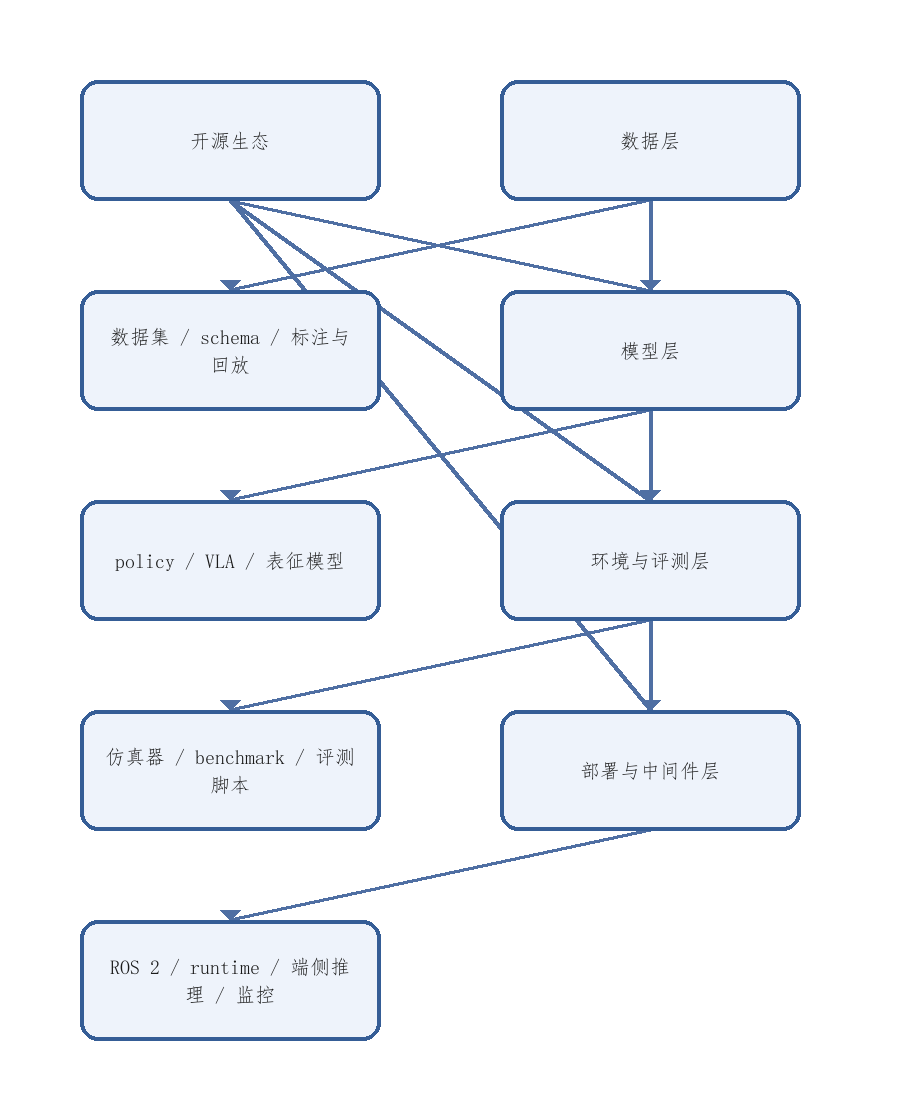
\includegraphics[width=0.9\textwidth,height=0.72\textheight,keepaspectratio]{figures/19-开源生态四层结构图.png}
\caption{19-开源生态四层结构图}
\label{fig:19-开源生态四层结构图}
\end{figure}

\chapter*{图表与案例补充}
\addcontentsline{toc}{chapter}{图表与案例补充}
\markboth{图表与案例补充}{图表与案例补充}

本章的图表与案例，不应被视为附属装饰，而应被理解为“如何把零散开源项目重新组织成学习与研究工作流”的结构化工具。对学习者来说，真正困难的往往不是知道仓库名称，而是判断一个项目位于数据、模型、环境还是部署层，并进一步识别它与自己研究目标之间缺失的工程链路。

因此，这里的补充材料应优先服务于接口关系、依赖方向、最小复现路径和失败模式分析，而不只是继续罗列项目名单。只有把这些关系显式画出来，开源生态才会从“很多仓库”转化为“可组合基础设施”。

在当前版本中，\texttt{\detokenize{图 19-1 开源生态四层结构图}} 已承担分层结构说明；19-代表性开源项目对照表 与 \texttt{\detokenize{表 19-1 开源生态四层对照表}} 则分别负责“项目级横向对照”与“生态层级定位”。

“从开源代码到最小复现实验”的路径，最好被理解成一类独立的研究资产，而不只是正文中的说明句。因为这类内容天然需要同时记录环境依赖、数据准备、训练命令、评测脚本和常见失败点，若只停留在报告叙述层，会很快丢失可复用性。因此，本章与 \path{research/}、\path{code/} 的连接并不是附属关系，而是开源章节真正能够服务后续实验工作的关键接口。

目前这章已经可以配合 19-开源生态四层对照表 和 19-代表性开源项目对照表 一起读。前者负责回答“开源生态分几层”，后者负责回答“具体项目在这几层中的什么位置、适合拿来做什么”。这样后续补项目时，就不容易重新退化成仓库名单。

\chapter*{表 19-1 开源生态四层对照表}
\addcontentsline{toc}{chapter}{表 19-1 开源生态四层对照表}
\markboth{表 19-1 开源生态四层对照表}{表 19-1 开源生态四层对照表}

\begingroup
\small
\begin{xltabular}{\textwidth}{YYYYY}
\toprule
层级 & 主要对象 & 关键问题 & 代表性项目/资产 & 主要局限 \\
\midrule
\endfirsthead
\toprule
层级 & 主要对象 & 关键问题 & 代表性项目/资产 & 主要局限 \\
\midrule
\endhead
数据层 & 采集、清洗、格式标准化、回放 & 数据是否对齐、可回流、可复现 & LeRobot、Open X-Embodiment、本地日志工具链 & 数据协议不统一、失败样本常不足 \\
模型层 & 感知 backbone、policy、VLA、world model & 输入输出接口是什么、动作表示是什么 & OpenVLA、Diffusion Policy、ACT & 模型可复现不等于可部署 \\
环境层 & 仿真器、benchmark、任务脚本、评测协议 & 奖励什么能力、忽略什么能力 & Isaac Sim、Habitat、MuJoCo、Gazebo & 平台差异导致结果难横比 \\
部署层 & ROS/中间件、端侧推理、监控告警、回放 & 能否稳定运行、可否诊断和回退 & ROS 2、edge runtime、monitoring stack & 开源资产常最薄、最难维护 \\
\bottomrule
\end{xltabular}
\endgroup

\chapter*{表 19-2 代表性开源项目对照表}
\addcontentsline{toc}{chapter}{表 19-2 代表性开源项目对照表}
\markboth{表 19-2 代表性开源项目对照表}{表 19-2 代表性开源项目对照表}

\begingroup
\small
\begin{xltabular}{\textwidth}{YYYYYY}
\toprule
项目 & 所在层 & 主要定位 & 输入输出接口关注点 & 更适合的使用阶段 & 主要局限 \\
\midrule
\endfirsthead
\toprule
项目 & 所在层 & 主要定位 & 输入输出接口关注点 & 更适合的使用阶段 & 主要局限 \\
\midrule
\endhead
OpenVLA & 模型层 & 开源 VLA 对照点 & 图像 / 语言 / 状态到动作接口 & 研究对照、接口理解、复现实验 & 离真实部署仍有明显系统差距 \\
LeRobot & 模型层 / 工具层 & 低门槛机器人学习与社区工作流 & 数据格式、训练调用、基础 policy 接口 & 学习、快速实验、社区复现 & 不能直接代表高复杂度生产级系统 \\
Open X-Embodiment & 数据层 & 跨平台机器人数据组织 & 跨机器人数据协议与样本组织 & 数据理解、基础模型训练前置 & 平台间动作和语义对齐仍然困难 \\
Diffusion Policy & 模型层 & 生成式动作学习基线 & 观测窗口到 action sequence / chunk & 动作建模研究、基线比较 & 部署时延与闭环恢复问题仍需额外系统补足 \\
ACT & 模型层 & 动作 chunking 路线代表 & 感知 + 状态到 chunked action & 操作策略基线、动作表示比较 & 需要结合系统约束解释其实用边界 \\
Habitat & 环境层 & embodied AI / 导航环境 & 环境实例化、任务 episode、评测协议 & 导航、场景交互、benchmark 研究 & 与真机接触和执行约束仍有距离 \\
Isaac Sim & 环境层 / 平台层 & 高保真仿真与平台生态 & 仿真、数据生成、训练-部署衔接 & sim2real、平台型开发工作流 & 平台依赖较强，不能自动等于真机闭环 \\
ROS 2 & 部署层 & 机器人中间件与系统总线 & 模块通信、QoS、日志、状态流 & 系统集成、部署、调试 & 不直接提供高层智能能力，需要与模型栈耦合 \\
\bottomrule
\end{xltabular}
\endgroup

从维护方法上看，后续新增开源项目时，建议先查 开源生态与工具链论文清单，再判断是否需要进入 19-代表性开源项目对照表 或 \path{data/processed/开源生态分层-v0.0.csv}。

% Generated from 20-企业分析框架.md; edit the LaTeX source after migration.

\reportpart{第二十部分 企业分析框架}
\addcontentsline{toc}{part}{第二十部分 企业分析框架}
\markboth{第二十部分 企业分析框架}{第二十部分 企业分析框架}

在具身智能领域，企业信息极易沦为新闻流和 demo 流。如果没有统一分析模板，就很容易被融资额、宣传片和单次演示带偏，而忽略真正决定长期价值的技术与交付变量。因此，本部分的职责，是先建立一个稳定的企业分析框架，再在后文具体公司章节中重复使用。

这一框架的必要性在 2024-2026 年尤为突出。Figure、Physical Intelligence、Apptronik、Agility、1X、Sanctuary AI、特斯拉 Optimus、优必选、宇树、智元等公司分别站在“通用本体”“VLA/基础模型”“工业交付”“物流场景”“人形平台”“远程接管”和“中国制造链协同”等不同位置上。若没有统一模板，很容易把风格完全不同的公司放在同一维度上比较，最后只剩下谁更会讲故事、谁视频更好看，而看不见底层变量。相关公司主页可参见 \href{https://www.figure.ai/}{Figure 官网}、\href{https://www.physicalintelligence.company/}{Physical Intelligence 官网}、\href{https://agilityrobotics.com/}{Agility Robotics 官网} 与 \href{https://www.ubtrobot.com/}{优必选官网}。

更进一步说，企业分析框架的真正意义不是“做成一张表”，而是把企业研究从新闻消费转成结构化判断。报告后续任何一版更新，只要能坚持使用同一套问题集，就能够积累跨时间、跨公司、跨路线的比较能力，而不是每次都重新被新的品牌叙事带走。

\section*{95. 为什么企业需要统一分析模板}
\addcontentsline{toc}{chapter}{95. 为什么企业需要统一分析模板}
\markboth{95. 为什么企业需要统一分析模板}{95. 为什么企业需要统一分析模板}

\subsection*{95.1 防止沦为新闻罗列}
\addcontentsline{toc}{section}{95.1 防止沦为新闻罗列}


企业分析最常见的失效方式，就是把连续发生的融资、发布会、合作新闻和 demo 视频顺次堆进报告，最后得到一份“信息很多但判断很弱”的时间流。之所以需要专门强调这一点，是因为具身行业本身就处在高波动、高叙事密度阶段，如果没有稳定框架，研究者很容易在更新过程中被最新事件牵着走，而丢失对企业长期能力结构的判断。

更稳健的做法，是把任何新增新闻都强制回写到既定分析维度中，例如它究竟改变了数据获取、系统集成、制造交付、客户进入还是资本耐心。只有当事件真正改变其中某一条能力链条时，它才值得进入正文判断；否则，它更适合作为跟踪日志而不是结构性结论。这个规则看似保守，但正是防止企业章节退化成“资讯摘要”的关键。 企业分析框架首先要解决的，就是避免把研究写成“按时间顺序堆新闻”。新闻罗列最大的问题不只是冗长，而是它会把高频曝光误当作高价值进展，把单次演示误当作能力跃迁。一个稳定框架的意义，在于无论企业发了多少视频、融资稿和发布会材料，我们都始终用同一组问题去过滤信息。

更具体地说，每条企业信息至少都应被追问三件事：它说明的是能力、接口、落地还是资本信号；它是一次性展示还是可重复趋势；它对应的证据强度来自论文、开源、客户部署还是市场宣传。只有把这三层拆开，企业研究才不会被节奏带着走。 企业分析之所以极易滑向新闻罗列，是因为外部公开信息天然偏向“融资、合作、发布、演示”这些传播友好事件，而真正决定公司位置的底层变量反而更难直接被看见，例如数据闭环是否真实建立、现场部署是否持续、失败恢复是否被系统性吸收、供应链是否开始收敛。统一模板的价值，就在于强迫分析从传播事件退回到系统变量，而不是被舆论节奏牵着走。

没有统一框架，企业章节往往会退化为时间线式材料堆叠，难以横向比较。

因此，这一章最重要的产出并不是“这次列了哪些公司”，而是留下了一套之后每个季度都能继续用的问题集。后续企业更新若偏离这套问题集，章节质量就会迅速回落到新闻摘要层。

\subsection*{95.2 便于横向比较}
\addcontentsline{toc}{section}{95.2 便于横向比较}


横向比较的目标，不是给所有企业排一个简单名次，而是让它们在相同问题集下暴露各自真正强、真正弱的环节。具身领域里最常见的阅读错觉，是把基础模型平台、本体制造商、场景集成商、共享自治服务商和综合型人形公司直接并排讨论，最后只剩下“谁故事更大、谁视频更好看”。这样的写法看似覆盖很广，实际上并没有形成可复核的判断，因为这些公司解决的根本不是同一层问题。

因此，真正可用的横向比较要先做两步。第一步是“按角色分组”，即先判断一家公司的主销售对象究竟是什么：它是在卖模型接口能力、本体能力、数据闭环能力、场景交付能力，还是制造与运维组织能力。第二步才是“在共同维度上投影”。我更建议固定八个维度：团队背景、技术路线、数据与模型、本体与系统能力、目标场景、商业路径、资本与合作、风险与局限。这样做的意义，不是消除差异，而是把差异压回可以解释的位置。

若把单家公司写成一个粗向量，可以记作：

\begin{equation*}
\mathbf{v}_{\text{firm}} = [T, R, D, B, S, C, F, K],
\end{equation*}

其中，\(T\) 对应团队与组织背景，\(R\) 对应路线角色定位，\(D\) 对应数据与模型闭环，\(B\) 对应本体与系统能力，\(S\) 对应目标场景与任务单元，\(C\) 对应商业路径，\(F\) 对应资本与合作网络，\(K\) 对应关键风险。这个向量的意义不是为了精确算分，而是为了确保后续任何一家企业都必须回答同一组问题。只要问题集稳定，企业章节就不会因为公司叙事风格不同而失去可比性。

同一分析模板真正强制我们反复追问的是：它的主任务单元是什么，它的控制权掌握在哪一层，它的数据与失败回流是否成环，它能否把能力复制到客户现场。只有这些问题被同一口径回答，企业比较才不会退化成传播比较。

目前这套模板已经落成表格版本，见 20-企业统一分析模板。后续版本若要做季度更新，可直接配合 20-企业季度跟踪表模板 使用，把横向比较进一步转成可追踪字段。

\subsection*{95.3 便于后续版本更新}
\addcontentsline{toc}{section}{95.3 便于后续版本更新}


企业分析框架若不能服务后续版本更新，它就只是一份一次性阅读提纲，而不是长期研究工具。一个合格的模板，必须让我们在数月后面对新增论文、融资、客户、事故、合作与产品发布时，能够把新信息直接插回既有维度，而不是整章重写。换句话说，模板的价值不仅在于当下读起来整齐，更在于未来是否支持增量维护。

这要求框架把“长期稳定维度”和“短期变动信号”明确分开。前者包括技术路线、本体形态、主要场景、组织出身和商业模式；后者包括新版本模型、客户试点、季度融资、关键人变动与新演示。只有把两类信息分层存放，后续版本才可能回答三个更重要的问题：哪些事实变了，哪些判断没变，哪些判断需要修正。

因此，本章模板本质上也是版本控制模板。它让企业研究从“每次重写一篇简介”转成“沿同一问题集持续积累判断”。这对本项目尤其关键，因为后续企业章节数量会持续增长，若没有稳定模板，整书很快会被新资讯冲散结构。 企业章节还必须服务于后续版本维护。一个好的结构不是只对当前阅读顺手，而是能在几个月后行业变化时，快速把新增论文、产品、客户、融资和事故插回原有框架中，而不必整章重写。

也就是说，企业框架不仅是阅读工具，还是版本化维护工具。它要求我们把“长期稳定维度”和“短期变化信号”分开放置：前者例如技术路线、本体形态、主要场景；后者例如最新产品发布、合作进展、融资事件和关键人才变动。 从版本维护角度看，这一点尤其关键。只要模板稳定，后续更新就可以把“哪些事实变了、哪些判断没变、哪些判断需要修正”分开记录，而不是每次新开一轮研究都把企业重新写成一篇简介。这使报告能够逐渐积累一种跨时间的判断连续性，而不是不断被新一轮宣传材料刷新记忆。

有模板，后续版本就能按相同结构增量更新，而不是每次重写企业画像。从版本维护角度看，企业分析框架也是报告长期可更新性的关键支点。它允许后续版本只替换“事实层”和“判断层”中的局部内容，而保留相同问题集，从而实现跨版本对照。

\section*{96. 企业统一分析维度}
\addcontentsline{toc}{chapter}{96. 企业统一分析维度}
\markboth{96. 企业统一分析维度}{96. 企业统一分析维度}

\subsection*{96.1 团队背景}
\addcontentsline{toc}{section}{96.1 团队背景}


团队背景之所以应被列为第一层，不是因为创始人履历天然决定成败，而是因为它往往提前暴露了公司最可能形成优势和最可能忽视的问题。来自自动驾驶、控制和机器人学背景的团队，通常更重系统安全、闭环与工程纪律；来自大模型或互联网 AI 背景的团队，往往更擅长统一接口、数据组织和平台叙事；来自制造或工业自动化背景的团队，则更可能在交付、成本和现场适配上走得更稳。

因此，阅读团队背景时最不该做的，是停留在“名校、名企、明星履历”的表层印象。真正值得追问的是：这支团队过去成功解决过哪一类复杂问题；它的知识结构是否覆盖了本体、数据、模型、部署与交付之间的关键断点；以及它是否存在明显的结构性盲区。例如强模型团队是否低估硬件与现场维护，强本体团队是否低估数据工程与持续学习。这些问题比头衔本身更接近企业未来路径。 团队背景不应只写创始人履历，而应回答“这家公司最初是从什么能力起家的”。控制、自动驾驶、计算机视觉、硬件制造、工业自动化、云平台或消费电子出身，会直接影响其早期技术路径、数据获取方式和商业切入点。

一个实用的读法是：团队背景往往不是花边信息，而是企业早期能力边界的线索。例如自动驾驶背景更容易延伸到感知栈和数据闭环，工业自动化背景更容易延伸到场景集成与客户交付，消费电子背景则更可能在成本工程和量产链条上占优。 团队背景之所以重要，不是为了满足公司介绍的完整性，而是因为它往往预示了路线的初始偏置。来自自动驾驶、工业自动化、消费电子、通用大模型、学术实验室或互联网平台的团队，会天然带着不同的问题拆解方式、风险偏好和工程优先级。理解这个出发点，往往能更早解释公司为何强调某类能力、忽略某类约束，以及其后续能否顺利跨越原有能力圈。

看创始人与核心团队是来自学术、工业自动化、自动驾驶、大模型公司还是消费电子，这往往会直接影响其技术与产品路径。

这一维度的重要性还在于，它通常能解释企业为何会优先解决某些问题、忽略另一些问题。团队背景不是花边信息，而往往是路线偏置最早也最稳定的来源之一。

\subsection*{96.2 技术路线}
\addcontentsline{toc}{section}{96.2 技术路线}


技术路线这一项的核心，不是给公司贴上“做 VLA”“做人形”“做世界模型”之类标签，而是判断它把哪一层能力当作主抓手。表面上许多公司都在讲“通用具身智能”，但真正决定路线分化的，往往是它把上限押在模型接口、本体平台、数据闭环、场景交付还是基础设施供给中的哪一环。若这一点不拆开，所谓路线比较就会退化成热词比较。

因此，技术路线分析至少要回答四个问题。第一，公司把系统上限主要押在哪一层。第二，这条路线最依赖什么稀缺资源，例如高质量遥操作、多机真数据、端侧算力、特定本体，还是高约束场景。第三，它的动作接口是什么，是连续控制、action chunk、技能 token，还是显式任务图。第四，一旦关键前提不成立，这条路线最可能以什么方式失效。只有把“主抓手-依赖条件-接口形态-失败模式”一起写出来，技术分析才真正具备判断力。

若把企业路线形式化地压缩，可以记为：

\begingroup
\scriptsize
\begin{equation*}
\mathcal{R}_{\text{firm}} = \bigl(L_{\text{primary}}, I_{\text{action}}, D_{\text{source}}, B_{\text{bottleneck}}\bigr)
\end{equation*}
\endgroup

其中，\(L_{\text{primary}}\) 表示主要押注层级，\(I_{\text{action}}\) 表示动作与控制接口，\(D_{\text{source}}\) 表示核心数据来源，\(B_{\text{bottleneck}}\) 表示最可能先暴露的瓶颈。这个写法的意义不在于追求伪精确，而在于迫使分析者不要只写“它用了什么模型”，而要写“它究竟靠什么赢，又可能先输在什么地方”。

按这个框架，当前企业常见的路线大致可以分为五类。第一类是“本体优先型”，核心优势来自执行器、整机一致性、机构设计和可制造性；它们的上限取决于身体平台能否稳定吸收更强智能。第二类是“模型接口优先型”，重点在于统一语言、视觉和动作接口，把更多任务组织权交给高层模型。第三类是“数据闭环优先型”，它们未必最强调某个模型名字，而更强调真机回流、失败吸收和持续重训。第四类是“场景交付优先型”，它们更像把具身系统包装成可卖的任务单元，而不是先追求跨场景通用性。第五类是“基础设施优先型”，如仿真、训练平台、端侧算力和工具链提供者，它们本身未必直接卖机器人，却在定义行业可用接口。

这五类路线并不互斥，但通常每家公司只有一类主轴最强。真正高质量的路线判断，不是简单说“它几类都做”，而是识别哪一类是其现金流、组织能力和技术叙事真正围绕的中心。以 Figure 在 2025 年发布的 Helix 为例，其官方说明强调的是通用 VLA、双系统分层、低功耗端侧部署和高频全上肢控制，这说明它当时的主轴不是单纯“做人形”，而是“以统一模型接口重写动作组织方式”，同时保留高低频分层这一工程妥协。\href{https://www.figure.ai/news/helix}{Figure Helix 官方说明}

同样地，技术路线的真正比较单位不是“是否用了大模型”，而是“输入是什么、动作接口是什么、低层保留了多少显式控制”。若一家公司仍然强依赖刚性技能库、固定工位和显式状态机，它更接近场景交付路线；若它把语言目标、历史状态和连续控制尽量压进统一模型，它更接近模型接口路线；若它大量资源投入在采数、回放、失败标签和后训练，则它更接近数据闭环路线。把这些接口层写清楚，往往比反复罗列模型名更有信息量。

因此，本章建议后续每个企业专题都沿同一组字段回写技术路线：主押注层、动作接口、主要数据源、最低层保留控制、部署前提、最可能失效位置。只要这些字段被固定下来，后续版本更新就不会因为企业改了几句宣传话术就失去比较坐标。

\subsection*{96.3 数据与模型能力}
\addcontentsline{toc}{section}{96.3 数据与模型能力}


企业的数据与模型能力，不能只停留在“有没有 foundation model”“有没有数据闭环”这类口号式描述，而要继续追问两者之间是否形成了可放大的耦合关系。公司究竟依赖公开多模态先验、遥操作示教、真实部署回流、仿真合成，还是多源混合；模型究竟服务于高层任务接口、技能调度、低层动作生成，还是更多停留在演示层。

更细一点，可以把所谓“数据与模型能力”拆成四个层次来判断。第一层是数据获取能力，即企业是否能够以可持续成本采集到高价值样本，而不是只靠一次性 demo 数据。第二层是数据组织能力，即是否具备标注规范、失败回放、质量筛选和跨任务复用机制。第三层是模型吸收能力，即这些数据究竟能否转化为更强的泛化、恢复或效率表现，而不是仅提升同分布指标。第四层是部署回流能力，即模型上线后产生的新数据是否还能重新进入训练与验证闭环。

只有当这四层形成正反馈时，数据与模型才真正构成企业壁垒。否则就会出现两种常见错觉：一种是“有很多机器人在跑，所以一定有数据优势”，但这些数据并未被结构化整理；另一种是“发布了大模型，所以模型能力一定领先”，但模型并未深度嵌入执行链路。报告在评估企业时，应当特别警惕这两类叙事捷径。

真正值得识别的是：企业是否具备把数据持续转化为模型改进、再把模型改进稳定反馈回部署表现的能力。若没有这条闭环，所谓“模型能力强”很可能只是阶段性亮点，而不是持续优势。反过来，即使模型名词不够响亮，只要数据回流、失败吸收和任务重训机制足够扎实，也可能形成更耐久的竞争力。

因此，这一维度在后续企业分析里建议至少记录五项：数据来源结构、数据回流频率、训练对象层级、是否覆盖失败样本、模型更新是否进入真实执行链路。只有这几项被写清楚，“数据与模型能力”才不是抽象标签，而是可比较变量。

企业的数据与模型能力，不应只看“有没有大模型”或“有没有数据闭环”这类口号式表述，而应继续追问这两者之间是否形成了真正可放大的耦合关系。公司究竟是依赖公开视频先验、遥操作示教、真实部署回流、仿真合成，还是多源混合？模型究竟服务于高层任务接口、技能调用、低层动作生成，还是更多停留在展示层？

也就是说，这一维度真正想识别的是：企业是否具备把数据持续转化为模型改进、再把模型改进持续反馈回部署表现的能力。若没有这条闭环，所谓“模型能力强”很可能只是一时亮点，而不是持续优势。 这一维度要看的，不只是“有没有模型”，而是数据闭环是否真实存在。具体可以追问：公司靠什么采数据，是真机日志、遥操作示教、仿真合成还是外部多模态数据；训练对象是技能策略、VLA、世界模型还是混合系统；模型更新是否看得出和部署反馈形成闭环。 这一维度不应只看“有没有大模型”或“有没有数据”，而要看两者是否形成闭环。公司是依赖公开数据、遥操作示教、现场日志回流，还是仿真合成与人工标注混合？模型是作为宣传层能力展示，还是已经进入真实执行链条？很多企业在这一维度最容易出现错觉：看起来模型很强，但没有足够真实闭环数据支撑；或者有不少现场数据，却缺乏统一表示层把数据资产真正放大。

看其是否掌握大规模真机数据、遥操作体系、仿真数据生成能力、foundation model 能力或特定任务闭环。

\subsection*{96.4 硬件与系统能力}
\addcontentsline{toc}{section}{96.4 硬件与系统能力}


硬件与系统能力必须单列，是因为具身企业最终交付的不是一个孤立模型，而是带本体、执行器、传感器、控制栈、中间件与运维边界的完整系统。若企业只在高层智能上发力，却无法控制本体一致性、执行器表现、现场标定和版本回滚，它的能力上限就很难在真实场景里兑现。

更有意义的追问不是“它有没有自己的机器人”，而是“它掌握了身体与智能之间哪些关键耦合位置”。哪些部件自研，哪些接口可控，哪些系统性风险由自己承担，哪些仍依赖外部平台，这些才决定企业究竟是展示型团队、集成型团队，还是具备系统主导权的产品团队。

这也是区分“模型公司借机器人做展示”和“真正具身公司”的关键维度之一。只要企业开始认真承担本体一致性、维护便利性、控制可靠性和现场部署摩擦，它面对的问题就从单点算法问题跃迁为系统工程问题。虽然这会拖慢节奏、增加成本，但也更接近真实交付能力。

硬件与系统能力之所以必须单列，是因为具身企业最终不只是交付一个模型，而是在交付一个带身体、带传感器、带控制栈、带运维边界的完整系统。若公司只在高层智能上用力，却无法控制本体一致性、执行器表现、中间件稳定性和现场部署摩擦，它的能力上限就很难真正兑现。

因此，看硬件与系统能力时，更有意义的不是问“它有没有自己造机器人”，而是问它是否真正掌握了身体与智能之间的关键耦合位置：哪些部件自己定义，哪些接口自己控制，哪些系统风险自己承担。只有这样，这一维度才不会退化成“有无本体”的表面判断。 硬件与系统能力这一栏的重点，是判断企业到底是在“借用通用平台堆模型”，还是确实掌握了本体设计、执行器、传感、控制和系统集成能力。很多企业看起来都能做演示，但真正决定持续交付能力的，往往是本体一致性、维护便利性、控制可靠性和现场适配能力。 这也是区分“模型公司借机器人做展示”和“真正具身公司”的关键维度之一。只要企业开始控制本体、执行器、传感配置、系统中间件、运行时监控与现场调度，它面对的问题就从单点算法跃迁为系统工程问题。虽然这会显著拖慢节奏、增加成本，却也更接近真实交付能力。很多公司真正的分水岭，不在 demo 有多亮眼，而在是否愿意承担这部分复杂性。

看其是否只是发布模型或 demo，还是已经控制本体、执行器、感知栈、中间件与运维链路。

\subsection*{96.5 产品与落地}
\addcontentsline{toc}{section}{96.5 产品与落地}


本节在企业分析里尤其重要，因为很多公司表面上“技术相似”，实际却在卖完全不同的东西。有的卖本体，有的卖整站解决方案，有的卖持续运维服务，有的卖数据与训练基础设施，还有的卖高层接口与生态位置。若不先把产品边界写清楚，后面的技术判断和商业判断很容易混线。

因此，记录产品与落地时，不应只写公司“做什么”，而应写客户“到底买到了什么”。客户买到的是设备、任务完成能力、持续升级承诺，还是一个可接入现有流程的中间平台？不同答案对应不同的销售周期、责任边界、实施难度与毛利结构，这些差异往往比模型名词本身更能解释企业走向。

产品与落地这一维度真正想回答的，不是企业“有没有产品名”，而是它到底卖的是什么交付单元。是本体平台、整套解决方案、按场景收费的服务，还是仍主要停留在技术验证和试点合作阶段。只有把交付单元定义清楚，后续关于客户、收入、部署规模和扩张性的判断才有意义。

这也是为什么企业分析中最容易被忽视的，并不是技术细节，而是产品边界。很多看起来都在“做机器人”的公司，实际上卖的是完全不同的东西；若不先把这一层拆开，横向比较就容易失真。 产品与落地不能只看“有没有发布产品名”，而要看它究竟对应什么交付单元。是卖硬件本体、卖整套解决方案、卖服务合同，还是先以试点项目形式进入客户现场？研究报告里，这一节最重要的是判断落地是否进入了重复部署阶段，而不只是单次合作展示阶段。 产品与落地维度的核心问题，是公司究竟卖什么。如果卖的是平台，本体、SDK、开发接口与生态协同就重要；如果卖的是场景方案，任务边界、部署稳定性和维护效率更重要；如果还停留在技术验证阶段，那么再漂亮的能力展示也不能直接外推为可规模化产品。把“卖什么”问清楚，很多表面相似的企业会立刻分流到完全不同的比较赛道上。

看其究竟在卖平台、整机、场景方案还是尚处于技术验证阶段。

\subsection*{96.6 资本与合作}
\addcontentsline{toc}{section}{96.6 资本与合作}


资本与合作信息之所以值得单列，不是因为它们能直接证明技术先进，而是因为它们会放大或暴露企业最核心的组织约束。一个合作若只是联合发布和品牌站台，信息含量并不高；若它开始改变数据来源、量产节拍、客户触达、关键零部件获取、场景试点或责任分工方式，它才真正进入企业能力层。

因此，资本与合作更适合作为“能力放大器”来读，而不是“结果证明”。更稳妥的读法，是先问这笔钱或这段合作穿透了哪一个原本最难突破的瓶颈。它究竟带来了真实场景、供应链位置、端侧算力、渠道入口、客户验证、标准话语权，还是只带来了市场注意力。只有能回答这个问题，资本与合作信号才不会把企业研究拖回“看金额、看名单”的叙事层。

在实践中，我更建议把资本与合作分成五类。第一类是“资金续航型”，解决的是公司还能跑多久、能否维持研发和量产节拍。第二类是“场景入口型”，例如客户试点、联合部署和行业渠道合作，它决定公司是否能进入真实任务流。第三类是“供给增强型”，包括关键器件、制造、供应链和算力合作，它决定系统能否从 prototype 走向 product。第四类是“数据放大型”，即是否让企业获得更多真机样本、失败回流或遥操作入口。第五类是“叙事放大型”，它主要增强关注度和市场预期，但不一定立即改变能力结构。

这一分类能帮助后续版本维护时避免两种常见误判。第一种误判是把大额融资直接等价于技术成熟；第二种误判是把知名合作伙伴直接等价于商业闭环。事实上，这两者通常只是能力形成的前置条件。真正值得上修判断的，是资本或合作是否已经把某个关键短板从“根本做不到”推进到“开始可组织地做到”。若没有这一层穿透，再漂亮的合作名单也应只作为辅助证据。

一个简单的阅读顺序可以写成：

\begingroup
\footnotesize
\begin{equation*}
\text{Signal Value} \propto \text{Bottleneck Penetration} \times \text{Execution Depth}
\end{equation*}
\endgroup

这里的含义很直接。若一笔合作同时穿透了真实场景、供应链和数据回流，且已经进入可执行阶段，它的权重就高；若它只停留在概念对齐、联合发布或模糊试点，它的权重就应显著降低。这个框架也解释了为什么同样叫“合作”，有的值得重写正文判断，有的只配进入季度日志。

具体到后续企业复审，建议固定记录至少六个字段：合作对象类型、改变的能力层、是否进入真实部署、是否改变数据来源、是否改变制造或供应链条件、是否改变客户获取方式。这样资本与合作就不再是新闻栏，而会成为“组织约束是否被改写”的结构化证据。

\subsection*{96.7 风险与局限}
\addcontentsline{toc}{section}{96.7 风险与局限}


这一项是企业分析里最不能礼貌化处理的一栏。具身领域最常见的误判，不是完全看错某家公司，而是只记住它最亮的一面，却没有写出它最脆的一面。每家公司通常都有一个在未来 12-24 个月内最可能主导上限的瓶颈，例如本体成本、采数效率、部署稳定性、运维网络、客户场景泛化、认证责任链或商业闭环。只有把这个瓶颈明确写出来，企业分析才真正具备判断力。

更进一步说，风险与局限不应写成泛泛的“行业仍早期、商业化仍有挑战”。真正有用的写法，应尽量指出哪一类约束最可能先成为拐点。例如，示教和清洗成本会不会先压垮扩张速度，端侧算力与热设计会不会先限制模型升级，现场运维和备件体系会不会先吞噬毛利，还是责任边界与客户验收条件会先阻断放量。风险写得越具体，后续版本越容易验证它是否正在变成现实。

我更建议把“风险”写成“主导瓶颈函数”，即不是罗列一串缺点，而是明确指出哪一个瓶颈最值得优先跟踪。可粗略写成：

\begingroup
\footnotesize
\begin{equation*}
b^{*} = \arg\max_{b_i \in \mathcal{B}} \; P(b_i)\cdot I(b_i),
\end{equation*}
\endgroup

其中，\(P(b_i)\) 表示该瓶颈在未来一段时间内暴露为现实问题的概率，\(I(b_i)\) 表示其一旦发生对整条路线造成的影响强度。这个式子的价值不在于算数，而在于逼迫分析从“公司有哪些缺点”转向“哪一个缺点最可能真正决定路线成败”。

从企业角色看，主导瓶颈经常有明显差异。基础模型或平台型公司更容易受限于数据闭环和端侧部署接口；本体型公司更容易受限于制造、一致性、维护和成本工程；场景集成型公司更容易受限于复制性、现场定制化和客户成功体系；共享自治或服务型公司更容易受限于人机责任边界和服务毛利结构。也就是说，“风险”不是公司简介里附带的一句客套话，而是该公司最真实的路线边界说明书。

后续版本维护时，建议每家企业的风险栏至少记录三件事：当前主导瓶颈是什么，哪些可观察信号会触发上修或下修，以及若该瓶颈长期未被解决，最可能在哪一层失速。这样写之后，风险与局限这一栏就不再只是平衡叙述，而会成为跨版本最有价值的判断锚点。

\subsection*{96.8 五个最容易被忽视的维度}
\addcontentsline{toc}{section}{96.8 五个最容易被忽视的维度}


这五个维度之所以值得单独拎出来，是因为它们往往不在企业最愿意主动展示的层面。新模型、新视频、新融资更容易形成传播高潮；真实部署频率、失败恢复链路、本体迭代节奏、客户约束强度以及供应链与维护能力，则更接近企业真实生命线。也正因如此，它们比热点新闻更适合作为跨版本对照指标。

我建议后续长期跟踪时，把这五项固定为企业专题里的“隐性质量字段”：

\begin{enumerate}
\item 真实部署频率，而不是单次展示频率。它回答的是系统是否真的在现场被反复使用。
\item 失败恢复链路，而不是平均成功率。它回答的是系统出错后能否回到可运营状态。
\item 本体迭代节奏，而不是只看模型迭代节奏。它回答的是硬件路线是否在收敛。
\item 客户约束强度，而不是泛泛“行业合作”。它回答的是场景是否对应高价值、强需求、可验收的问题。
\item 供应链与维护能力，而不是单纯融资速度。它回答的是公司能否从 prototype 过渡到 product。
\end{enumerate}

这五项高价值的原因，在于它们更接近“真实系统能否长期活着”，而不是“外部是否觉得它很厉害”。例如，部署频率反映客户是否真的愿意把系统纳入流程；恢复链路反映系统是不是具备闭环韧性；本体节奏反映机械、电气、驱控和制造是否同步收敛；客户约束强度决定它做的到底是高价值真问题还是概念展示；维护与供应链能力则决定规模化是不是会在交付阶段崩塌。

从长期版本维护角度看，这五项还有一个额外优点：它们通常比热点叙事更稳定，更适合做趋势比较。谁在这些字段上持续改善，谁的进步往往更接近系统性进步；谁只在声量、估值或论文数量上增加，却在这些字段上长期空白，其真实位置就应更谨慎判断。

若进一步制度化，这五个维度完全可以直接写入企业季度跟踪卡的固定字段。这样后续更新时，不必再凭印象判断“这家公司最近有没有进步”，而是直接看部署频率、恢复链路、本体节奏、客户约束和维护能力是否出现连续改善。对长期研究项目而言，这种字段化比任何一次性的企业长评都更有复用价值。

\section*{97. 如何识别“炫技 demo”与“可交付能力”}
\addcontentsline{toc}{chapter}{97. 如何识别“炫技 demo”与“可交付能力”}
\markboth{97. 如何识别“炫技 demo”与“可交付能力”}{97. 如何识别“炫技 demo”与“可交付能力”}

\subsection*{97.1 视频展示常见误导}
\addcontentsline{toc}{section}{97.1 视频展示常见误导}


视频最大的风险不在于一定造假，而在于它天然会省略对判断最重要的背景信息。常见被省略的内容包括：总尝试次数、失败率、人工摆放与复位、远程接管、灯光与障碍物条件、异常恢复过程以及单位时间产出。也就是说，视频最容易展示的是“能力上界片段”，而不是“能力分布样本”。

因此，阅读 demo 的更好习惯不是先赞叹动作是否流畅，而是先写下几个反向问题：这里被筛掉了哪些失败，这里的人类劳动被转移到哪里去了，这里的环境条件有多受控，这里的成功一次究竟花了多少时间。只有把这些问题固定下来，视频材料才会从宣传内容变成研究证据。

视频展示最强的地方，是它能快速传递能力上限；最弱的地方，是它几乎总会隐藏能力分布。观众往往能看到一个系统“最好时刻能做到什么”，却看不到它失败了多少次、重试了多少轮、是否存在人工介入、环境是否经过专门准备，以及这一能力是否能在其他场景稳定复现。

因此，视频不是没价值，而是必须被放在更严格的证据层级下使用。它可以作为线索，但不应直接当作结论。真正高质量的企业判断，必须继续追问视频背后看不见的那些变量。 企业视频常见误导至少包括四类：只展示最优片段、不展示失败率；通过剪辑弱化等待、重试与人工介入；隐藏环境约束与任务预处理；用自然语言叙述夸大系统自主程度。报告在解读视频时，必须先把这些可能性放到前台，而不是先接受视频叙事。 公开视频最大的误导，不在于它一定造假，而在于它天然选择性呈现。视频几乎从不展示失败率、重复试验次数、场景准备成本、人工介入比例、远程接管强度和异常恢复过程。也就是说，视频更像能力上界片段，而不是能力分布样本。若不主动补问这些缺失信息，就很容易把“最优一次”误读为“平均水平”。

公开视频通常天然筛掉失败案例、场景准备成本和重复试验次数，因此绝不能直接等同于真实平均能力。

\subsection*{97.2 真正值得看的技术与商业指标}
\addcontentsline{toc}{section}{97.2 真正值得看的技术与商业指标}


真正值得看的指标，往往都比宣传口径更“无聊”，却也更接近系统现实。企业最愿意主动展示的，通常是动作顺滑、一次完成、视觉冲击强的演示友好指标；研究者真正该长期盯住的，则是恢复率、接管率、连续运行时长、单位场景复制成本、维护负担、版本回归稳定性和客户续约情况。前者更容易出现在视频里，后者更接近“系统能否活在现实里”。

如果把指标体系压缩成一个最实用的研究面板，我更建议至少分成四层。第一层是任务层指标，回答“它会不会做”：任务完成率、任务节拍、单位时间产出、动作覆盖面。第二层是恢复层指标，回答“失败后怎么办”：恢复成功率、平均接管次数、异常分类完备性、回退路径是否明确。第三层是运维层指标，回答“能不能长期跑”：连续运行时长、版本回归故障率、维护工时、现场标定频率、硬件替换后是否需要重新大规模调试。第四层是商业层指标，回答“值不值得持续买”：单场景复制成本、部署周期、客户扩点速度、续约率和单位产能提升。

形式化地说，可以把真正高价值的指标写成：

\begingroup
\scriptsize
\begin{equation*}
\mathcal{M}_{\text{deliver}} = \{m_{\text{task}}, m_{\text{recovery}}, m_{\text{ops}}, m_{\text{economics}}\}
\end{equation*}
\endgroup

其中，\(m_{\text{task}}\) 衡量能力上限，\(m_{\text{recovery}}\) 衡量韧性，\(m_{\text{ops}}\) 衡量系统化运行能力，\(m_{\text{economics}}\) 衡量商业兑现质量。这个分法的好处是，任何企业即使某一维非常亮眼，也必须同时回答其余三维是否成立。否则，判断很容易被单点强项误导。

在企业比较中，我尤其建议优先看那些“宣传层最难伪装”的变量。例如单个任务能否连续多小时运行、出错后是否靠模型闭环恢复还是靠人工接管、同一系统能否在相近客户之间快速复制、是否已经形成明确维护接口、以及模型更新是否真的进入现场迭代闭环。这些变量比“模型更强了”“机器人更灵巧了”更能解释中期竞争格局。

这一点其实已经能从当前较成熟的工业与巡检产品页面里看到。以优傲机器人（Universal Robots）为例，其官方产品页强调的是协作机械臂的安全、灵活、易部署、易编程和可扩展性，并进一步区分不同系列在性能、可靠性和服务体系上的差异。这种表述的中心不是一次演示动作，而是部署、维护和复制能力。\href{https://www.universal-robots.com/products/}{优傲机器人官方产品页} 同样地，波士顿动力（Boston Dynamics）对 Spot 的介绍重点放在动态感知、工业巡检、危险环境进入、自动充电、动态重规划、自扶正和企业级部署支持上。这些字段都更接近“交付友好指标”，而不是“演示友好指标”。\href{https://bostondynamics.com/products/spot/}{波士顿动力 Spot 官方产品页} 这也说明，真正值得长期记录的，往往是系统如何被持续交付，而不是它曾经做出过多精彩的一次动作。

因此，一个更实用的企业指标纪律是：先把指标分成“演示友好”和“交付友好”，再看两者之间是否一致。若企业只持续给出前者，而长期不给出后者，那么判断应自动保守；若它开始稳定给出连续运行、恢复、维护和复制相关证据，即使模型叙事并不花哨，也值得上修其成熟度判断。对长期版本维护而言，这种指标分层比任何单次企业长评都更可复用。

\subsection*{97.3 从工程稳定性判断成熟度}
\addcontentsline{toc}{section}{97.3 从工程稳定性判断成熟度}


从工程稳定性判断成熟度的核心逻辑，是把“最亮眼的一次表现”降权，把“在更长时间、更大样本、更复杂条件下持续成立的能力”升权。系统是否能连续运行、是否能在干扰下恢复、是否能在不同客户现场重复部署，这些都比一次视频中的高光时刻更接近成熟度。

进一步说，工程稳定性最值得看的不是单个指标，而是一组彼此关联的运维信号：异常是否可分类、接管边界是否明确、部署脚本是否标准化、硬件替换后是否需要大规模重新标定、回归测试是否能覆盖典型任务、版本升级是否会引入新型现场故障。一个系统即便在研究演示中很强，如果这些基础信号长期缺位，其成熟度判断也应显著保守。

这也是为什么一些公司看起来“技术味”没那么浓，却可能更接近商业成熟。因为它们在故障处置、现场服务、备件体系、软件发布节奏和客户成功机制上建立了稳定流程。具身智能作为系统产品，最终竞争的不只是算法峰值，而是谁更能把复杂能力压缩成可复制交付的工程组织能力。

这并不是否认单次技术突破的意义，而是强调具身行业里真正昂贵的往往不是能力峰值，而是能力分布。一个成熟系统未必最惊艳，但通常更克制、更稳定、也更可预测。 工程稳定性往往比“单次能力峰值”更能代表企业成熟度。一个系统若只能在高度筛选的场景里偶尔表现惊艳，而无法在连续运行、边缘案例和维护约束下稳定工作，其商业价值通常仍然有限。

因此，成熟度判断应更多追问连续运行时长、失败恢复链路、现场运维机制、版本更新频率和场景复制成本，而不是只问“它能不能做出这个动作”。 成熟系统的一个典型特征，是它在视频里往往显得克制。动作更保守，节奏更均匀，异常处理更明确，系统行为更像围绕可持续运行优化，而不是围绕一次展示最优效果优化。很多时候，正是这种“不炫”才说明系统已经开始认真面对现场约束，而不再只是追求视觉冲击。

一个真正成熟的机器人系统，往往在视频里看起来不一定最“惊艳”，但在结构、动作、节奏和异常处理上会表现出更强的工程克制感。

从分析训练角度看，这一点非常值得刻意练习。对同一段企业视频，最好强迫自己额外写下几条“看不见的信息需求”：是否经过多次重试、是否有人远程介入、是否限定了对象与环境、是否有任务失败后恢复、是否有长时运行证据。只要长期保持这种逆向提问，企业章节的判断质量会比单纯追新闻显著更稳。

\subsection*{97.4 一个更实用的判断顺序}
\addcontentsline{toc}{section}{97.4 一个更实用的判断顺序}


与其先问“这家公司是不是在做 AGI for robotics”，不如先按一条更克制的顺序判断：

\begin{enumerate}
\item 它解决的是哪一类任务单元。
\item 这些任务单元是否具有稳定价值密度。
\item 它是否建立了真实数据与失败回流。
\item 它是否能把能力交付到客户现场。
\item 它的长期平台潜力是否有证据支持。
\end{enumerate}

这套顺序的价值，在于它先压住想象空间，再讨论上限空间。许多企业之所以容易被高估，并不是因为故事一定错误，而是因为分析顺序倒了过来：先被宏大平台叙事吸引，再回头补看任务入口、失败回流与部署现实。一旦顺序固定，企业章节的判断稳定性就会显著提高。

如果把这一顺序写成证据加权框架，可以暂时压缩为：

\begingroup
\footnotesize
\begin{equation*}
S_{\text{firm}} = w_t T + w_d D + w_s S + w_m M + w_c C - w_r R,
\end{equation*}
\endgroup

其中，\(T\) 表示任务单元是否清晰，\(D\) 表示数据与失败回流是否成环，\(S\) 表示系统交付成熟度，\(M\) 表示模型与接口的可迁移性，\(C\) 表示客户黏性与持续付费能力，\(R\) 表示安全、制造、组织与现金流风险。这个式子的作用不是生成排行榜，而是强制每个分量都绑定到具体证据。

更稳健的做法，是再给每个分量附一个证据等级 \(\scriptstyle e \in \{\text{story}, \text{demo}, \text{pilot}, \text{deployment}, \text{operations}\}\)。同样是“交付能力强”，如果证据只停留在公开视频，和已经有跨站点连续运行记录，研究判断的权重完全不应相同。也就是说，本章真正想固定下来的，不是公司名次，而是“证据先于叙事”的比较纪律。

若把它进一步压缩成可执行的研究流程，可以写成：

\begin{lstlisting}[language=python]
def screen_company(firm):
    if firm.task_unit is None:
        return "story risk"
    if firm.failure_loop is None:
        return "demo risk"
    if firm.deployment_evidence < 2:
        return "delivery risk"
    if firm.manufacturing_plan is None and firm.embodiment_heavy:
        return "scale risk"
    return "worth long-term tracking"
\end{lstlisting}

这段伪代码故意很朴素，因为企业分析的关键从来不是模型多复杂，而是先把误判挡在门外。对后续版本维护来说，任何新公司、新融资或新路线，只要能被这套“任务单元 - 失败回流 - 交付证据 - 规模化约束”的顺序重新过一遍，企业章的口径就不容易在热点切换中漂移。

这套顺序若要长期稳定使用，还需要再加一条纪律：先按固定问题拆公司，再决定它是否值得写长评，而不是反过来先被热点公司吸引再补框架。换言之，本章不是为了帮助我们“更会写公司简介”，而是为了让后续任何公司专题都先暴露其任务入口、数据闭环、交付能力、制造条件与主要风险，再决定叙事重心。

另一个很关键的点是，企业分析模板本身也应被视作一种“研究接口”。如果后续多轮维护发现某类企业反复落在当前模板缝隙里，例如基础设施平台、shared-autonomy 服务商或软硬件深度耦合型公司难以被现有字段解释，那么需要回调的就不只是单家公司判断，而是模板本身。也因此，本章并不是静态附录，而是后续企业章节能否长期保持可比性的前置条件。

\section*{图 20-1 企业分析流程图}
\addcontentsline{toc}{chapter}{图 20-1 企业分析流程图}
\markboth{图 20-1 企业分析流程图}{图 20-1 企业分析流程图}

\noindent\textit{源文件：\texttt{\detokenize{assets/diagrams/20-企业分析流程图.mmd}}}

\begin{figure}[htbp]
\centering
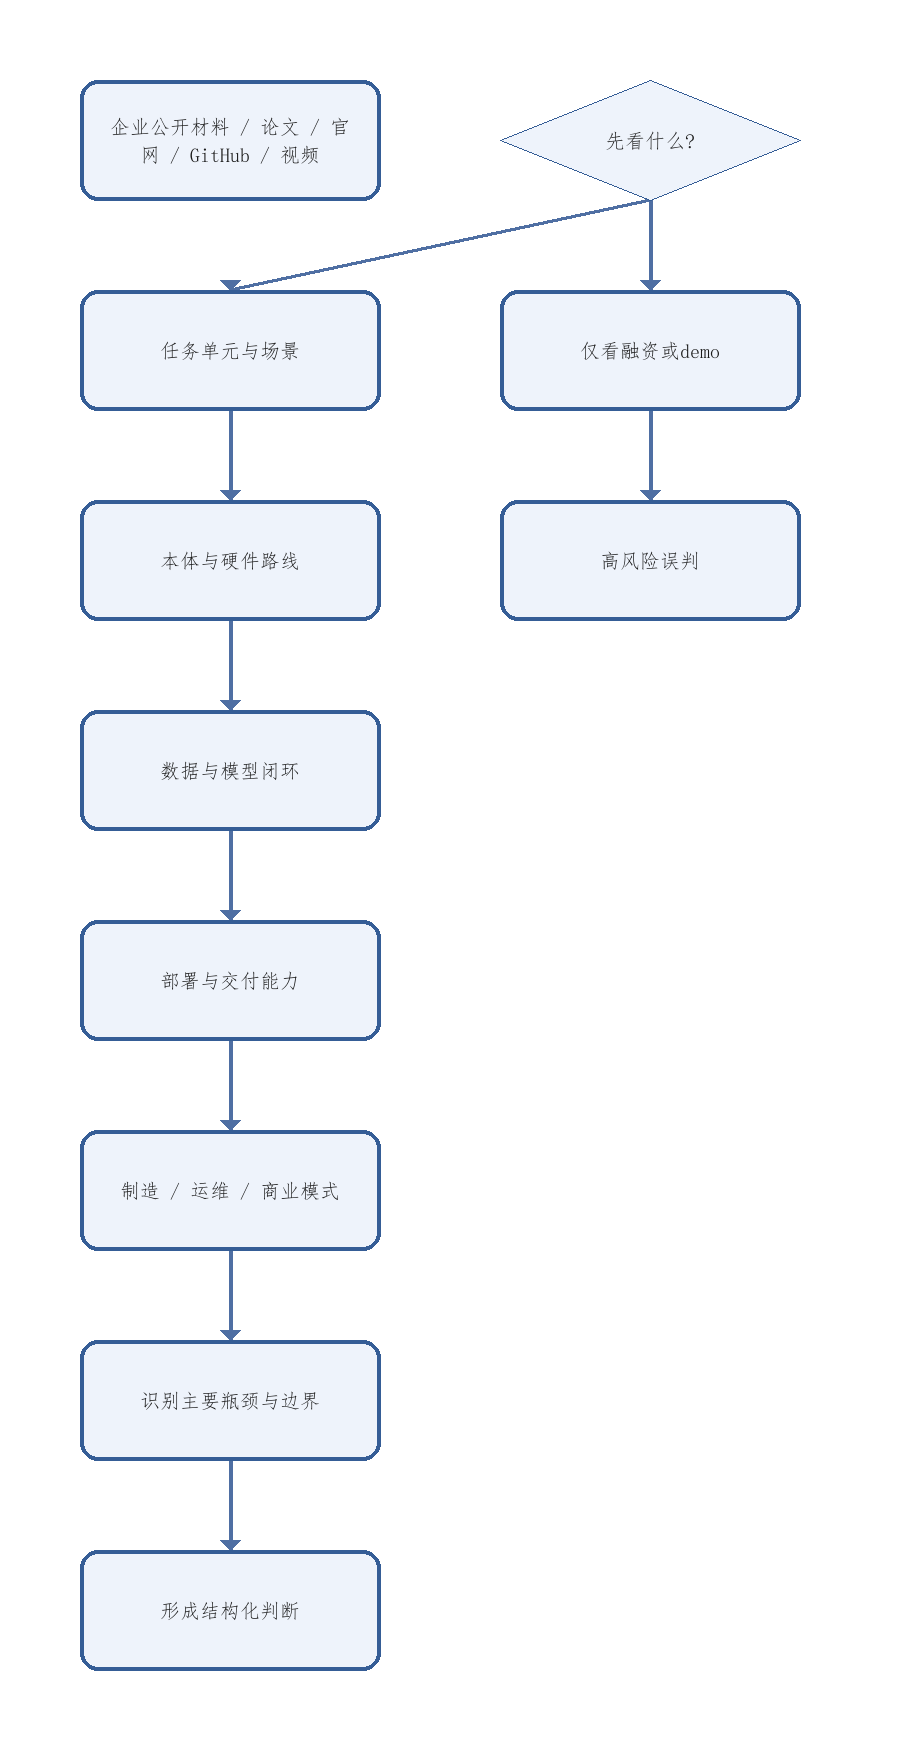
\includegraphics[width=0.9\textwidth,height=0.72\textheight,keepaspectratio]{figures/20-企业分析流程图.png}
\caption{20-企业分析流程图}
\label{fig:20-企业分析流程图}
\end{figure}

\section*{表 20-1 企业统一分析模板}
\addcontentsline{toc}{chapter}{表 20-1 企业统一分析模板}
\markboth{表 20-1 企业统一分析模板}{表 20-1 企业统一分析模板}

\begingroup
\small
\begin{xltabular}{\textwidth}{YYYY}
\toprule
维度 & 核心问题 & 典型证据 & 常见误判 \\
\midrule
\endfirsthead
\toprule
维度 & 核心问题 & 典型证据 & 常见误判 \\
\midrule
\endhead
本体 & 公司控制哪类本体？本体是否是核心护城河？ & 本体规格、负载、续航、自由度、末端执行器 & 只看外形，不看可制造性 \\
模型 & 是做 VLA、技能层、世界模型还是系统集成？ & 论文、博客、技术主页、模型接口 & 把高层语义能力当成完整系统能力 \\
数据 & 是否掌握高质量真机/遥操作/失败回流数据？ & 数据闭环描述、采集系统、数据集合作 & 只看“数据多”，不看数据类型和闭环 \\
部署 & 是否有真实场景、维护体系和恢复机制？ & 客户案例、试点、运维流程 & 把 demo 当部署 \\
制造 & 是否有供应链、量产、成本工程能力？ & 交付节奏、供应链合作、良率信息 & 把原型能力当量产能力 \\
商业模式 & 卖平台、整机、方案还是 RaaS？ & 收费模式、客户类型、合作方式 & 只看融资不看收入结构 \\
主要风险 & 当前最脆弱瓶颈在哪？ & 任务覆盖、成本、可靠性、法规 & 用宏大叙事遮蔽单点瓶颈 \\
\bottomrule
\end{xltabular}
\endgroup

\section*{图表与表格补充}
\addcontentsline{toc}{chapter}{图表与表格补充}
\markboth{图表与表格补充}{图表与表格补充}

这一章末尾之所以需要专门收束为模板、流程图和版本对照样例，是因为它的目标并不是“介绍企业”，而是建立一把可重复使用的分析尺子。没有统一模板时，不同企业极容易被各自的材料口径牵着走；只有先把问题集固定下来，后续企业章节才有可能在相同维度下比较本体、数据、部署、交付和风险。

从版本维护角度看，这组补充材料同样是后续更新工作的关键支点。以后更新企业章节时，最重要的不是重写公司简介，而是沿着同一模板替换事实层、修正判断层，并保留跨版本可对照性。

在当前版本中，\texttt{\detokenize{图 20-1 企业分析流程图}} 已承担“从外部信号进入可交付判断”的流程锚点职责；\texttt{\detokenize{表 20-1 企业统一分析模板}} 则把“本体 / 模型 / 数据 / 部署 / 制造 / 商业模式 / 主要风险”等横向比较维度固定下来。

“同一企业多轮版本更新如何回写判断层”这一问题，本质上要求报告具备跨时间的结构化记忆能力。单靠正文叙述很难稳定维护，因此更适合通过 20-企业季度跟踪表模板 与企业长期跟踪卡来承载。正文负责输出阶段性判断，结构化资产负责记录新增信号、口径变化和判断回调依据，两者结合后，企业研究才不会退化成一次性的公司简介。

为了让这一章真正变成后续维护的工作台，而不是只作为阅读框架存在，建议后续企业更新统一依赖两张表：一张是 20-企业统一分析模板，负责稳定横向比较维度；另一张是 20-企业季度跟踪表模板，负责记录季度新增信号与是否需要回调专题。这样做后，企业章节的更新路径就会从“重写公司简介”转变成“先补信号，再修判断”。

如果需要进一步降低后续维护成本，也可以直接优先使用脚本导出版：20-企业统一分析模板-脚本生成版 与 20-企业季度跟踪表模板-脚本生成版。其底层字段源位于 \path{data/processed/}，便于后续先改结构化字段，再统一导出到正文表格。

作为首批可复用研究资产，后续企业章节还应优先复用以下长期跟踪卡，而不是每次重新从新闻和视频开始：

\begin{enumerate}
\item Google DeepMind 长期跟踪卡
\item NVIDIA 长期跟踪卡
\item Figure 长期跟踪卡
\item 优必选 长期跟踪卡
\end{enumerate}

对于高频变化信号，后续不应直接在长期卡或正文里堆新闻，而应优先记入季度更新日志。当前已建立的样板包括：

\begin{enumerate}
\item 企业季度更新日志模板
\item Google DeepMind 季度更新日志
\item NVIDIA 季度更新日志
\item Figure 季度更新日志
\item 优必选 季度更新日志
\item Agility 季度更新日志
\item Apptronik 季度更新日志
\item 智元 季度更新日志
\item 宇树 季度更新日志
\end{enumerate}

如果后续要把季度信号沉淀到统一结构化表中，则应同步更新 20-企业季度跟踪表模板-脚本生成版 对应的底层 csv，而不是只在正文里补一句“本季度有变化”。

\input{chapters/21-海外重点企业专题}
\input{chapters/22-国内重点企业专题}
% Generated from 23-应用落地与商业化.md; edit the LaTeX source after migration.

\part*{第二十三部分 应用落地与商业化}
\addcontentsline{toc}{part}{第二十三部分 应用落地与商业化}
\markboth{第二十三部分 应用落地与商业化}{第二十三部分 应用落地与商业化}

技术路线能否成立，最终要回到场景。很多具身系统在实验室中都能展示能力，但只有少数能在特定场景中把能力、成本、稳定性和维护约束同时平衡出来。因此，本部分的重点不是重复场景分类，而是解释为什么某些场景更容易先跑通，以及商业化究竟被什么约束。这里最关键的判断标准不是“场景是否听起来足够宏大”，而是“场景是否允许局部结构化、是否能容忍有限失误、是否有足够高的价值密度去覆盖机器人系统成本”。

如果把应用落地问题抽象化，可以把单场景可行性理解为以下多因素函数：

\begingroup
\scriptsize
\begin{equation*}
\text{Viability} \approx f(\text{task structure}, \text{error tolerance}, \text{labor value}, \text{integration cost}, \text{maintenance burden})
\end{equation*}
\endgroup

这个表达式虽然不是严格商业模型，但足以说明一个现实：很多“技术上更炫”的场景，反而因为价值密度不足、误差容忍度太低或维护成本过高，而并不适合作为第一波商业化入口。

\chapter*{105. 制造业与仓储物流}
\addcontentsline{toc}{chapter}{105. 制造业与仓储物流}
\markboth{105. 制造业与仓储物流}{105. 制造业与仓储物流}

这仍然是当前最现实的落地方向之一。原因不是技术最简单，而是流程更容易局部结构化、ROI 更可量化、任务价值密度更高、现场维护体系更容易建立。也正因为如此，许多看起来“不够通用”的系统，反而更可能率先在这里形成真实价值。真正先跑出来的，通常不是“会做所有事”的机器人，而是能稳定接管某一类高频、高价值、可重复但又尚未被完全自动化的任务单元。仓储、分拣、搬运与工位协作也是 Agility、Amazon 等案例反复出现的主线。\href{https://agilityrobotics.com/}{Agility Robotics}、\href{https://www.aboutamazon.com/news/operations/amazon-tests-digit-humanoid-robot}{Amazon Robotics}

\section*{105.1 为什么这类场景总是反复领先}
\addcontentsline{toc}{section}{105.1 为什么这类场景总是反复领先}


制造、仓储、分拣与搬运场景之所以总是反复领先，并不是因为技术在这里最“先进”，而是因为它们最早满足了一组适合被交付的条件：任务可分解、价值密度高、收益可核算、失败可兜底、部署环境可被部分改造。也就是说，这类场景的优势不在于问题已经被彻底解决，而在于企业可以通过夹具、动线、工位约束、人工兜底和流程重组，把开放问题先压缩成一个可运营问题。

如果把场景落地能力抽象成一个粗略筛选式：

\begingroup
\scriptsize
\begin{equation*}
\text{Deployability} \propto
\frac{\text{task repetition} \times \text{value density} \times \text{verifiability}}
{\text{integration burden} \times \text{failure cost}},
\end{equation*}
\endgroup

那么制造与仓储的核心优势，通常不是分子绝对最大，而是分母更可控。它们允许企业逐步把复杂任务拆成高频、局部结构化的任务单元，只要系统能稳定接管其中一个高价值片段，就可能先形成真实商业收益。对商业化早期而言，这比一次性追求开放世界通用能力更重要。

更准确地说，这类场景长期领先的原因，是它们最适合做“运营压缩”：把原本散乱的感知、接触、恢复、验收和责任链，先压缩到一个客户能接受的范围内。只要企业能够把任务边界、异常处理、人工兜底和 ROI 计算稳定下来，它就在积累一种比单次模型性能更重要的能力，即“把机器人组织成可持续使用资产”的能力。

因此，本节最值得强调的判断不是“这些场景天然优质”，而是“这些场景最适合沉淀交付能力”。企业在这里真正建立的，往往不只是某个仓储或制造案例，而是一整套方法：如何定义任务单元、如何设计人工兜底、如何度量 ROI、如何把异常恢复流程写进运维模板、如何把单站点经验复制到第二个站点。这些能力一旦形成，才有可能外溢到更复杂场景。

从后续跟踪口径看，这类场景真正值得记录的也不是“又多了一个试点”，而是三类更硬的指标：第一，人工基线是否清楚，即原流程的人力、节拍和错误成本是否可量化；第二，机器人介入后是否把异常处理、夜班覆盖、危险工序或高波动工位稳定压下来；第三，第二站点复制时新增的工位改造、软件适配和运维负担是否明显下降。只有当这些指标持续改善时，制造与仓储场景的领先才不只是阶段性热度，而是交付组织能力的真实积累。

\section*{105.2 典型任务单元的判断标准}
\addcontentsline{toc}{section}{105.2 典型任务单元的判断标准}


任务单元判断之所以必须细到单元级，而不能停留在“行业/场景”级，是因为真正决定可商业化的往往不是整个行业是否需要机器人，而是某个具体工作片段是否足够结构化、是否容易度量收益、是否允许局部自动化先切入。仓储、制造、巡检、农业这些大类内部，往往同时包含适合早落地和暂不适合落地的子任务。

因此，任务单元的判断必须压到比“行业/场景”更细的层级。真正决定可商业化的，往往不是整个行业是否需要机器人，而是某个具体工作片段是否足够结构化、是否容易度量收益、是否允许局部自动化先切入。对制造与仓储场景，更有意义的不是泛泛说“机器人进工厂/仓库”，而是拆到搬运、上下料、分拣、包装、质检、巡检、工位协作这些最小闭环，再分别问它们需要什么感知、接触、时延与恢复能力。

把这套判断压缩成一个更工程化的筛选式，可以写成：

\begingroup
\scriptsize
\begin{equation*}
\text{TaskScore} =
w_1 \cdot \text{observability}
+ w_2 \cdot \text{repeatability}
+ w_3 \cdot \text{value density}
- w_4 \cdot \text{failure cost}
- w_5 \cdot \text{integration burden}
\end{equation*}
\endgroup

这当然不是为了制造一个可以机械打分的商业公式，而是提醒我们：一个任务单元之所以适合作为具身切入口，几乎从来都不是因为“模型已经足够强”这一条，而是因为观测、恢复、验收、付费和集成五个维度形成了相对有利的组合。很多演示看起来能做的任务，最后死在高失败代价和高集成摩擦；很多看起来不够性感的任务，则因为重复度高、收益明确而率先变成现实业务。

因此，后续评估任何任务单元时，最值得固定记录的问题只有五个：任务输入是否可感知，目标状态是否可验收，失败后是否存在低成本恢复路径，接入现有流程是否需要大规模改造，以及客户是否已经为该环节持续付钱。只有拆到这一层，本章才会真正成为商业判断工具，而不是对几个大行业的宏观赞美。

\chapter*{106. 家庭、消费级服务与医疗康复}
\addcontentsline{toc}{chapter}{106. 家庭、消费级服务与医疗康复}
\markboth{106. 家庭、消费级服务与医疗康复}{106. 家庭、消费级服务与医疗康复}

家庭和消费场景最接近“通用具身终局”，但短期最难规模化；医疗和康复则价值明确，但监管、责任和验证门槛极高。这两类场景都值得长期关注，但不应轻易被视为短期爆发主线。家庭场景最难的不是单个任务，而是开放度极高、语义模糊、对象多样、且任何失误都直接面向终端用户；医疗场景则最难在于即便技术能力不错，也必须先通过责任、流程和合规边界。

\section*{106.1 这两类场景为什么常被高估}
\addcontentsline{toc}{section}{106.1 这两类场景为什么常被高估}


家庭与医疗康复场景之所以常被高估，不是因为它们不重要，而是因为它们同时具备“高可见度”和“高终局想象力”。家庭直接连接大众生活，医疗康复直接连接高价值需求与社会善意，这使它们天然适合承载“未来生活方式改变”的叙事。但从部署角度看，这恰恰是两类最难被快速工程化的场景。

家庭场景的困难，在于开放环境、长尾物体、家庭成员干扰、儿童与宠物共处、长期售后和日常维护条件都远比工业现场复杂。医疗康复的困难，则在于责任链、伦理约束、流程嵌入、设备认证与人工接管边界必须同时成立。也就是说，这两类场景都不是“单次动作做出来”就能成立的场景，而是“整套责任体系和长期运维体系”必须共同成立的场景。

它们之所以被系统性高估，还有一个更隐蔽的原因：演示价值和商业价值在这里更容易被混写。家庭场景里，一个系统只要能在少数物体、少数房间、少数脚本中完成看起来“像生活”的任务，就足以获得极强传播效果；医疗康复里，只要机器人表现出对人体动作、护理流程或陪伴交互的某些片段能力，就会被天然赋予更高善意解读。但传播强化并不等于部署门槛下降。

因此，本章对它们采用“长期高价值、短期慢兑现”的判断口径。未来若出现声称在家庭或医疗康复场景取得突破的新系统，最值得优先核查的不是演示视频的流畅度，而是四类证据：开放环境鲁棒性、长期维护可行性、责任边界清晰度，以及真实用户条件下的长周期使用记录。只要这些证据还薄弱，就不应把它们直接写成短期主线。叙事强度在这里往往与短期可交付性反向相关，这是阅读相关新闻时最需要刻意校正的偏差。

更具体地说，家庭与医疗康复场景都存在一种“不可见人工被系统性低估”的问题。家庭产品往往需要复杂安装、远程客服、频繁地图重建与用户教育；医疗康复系统则更容易把医生、治疗师、护理员和合规团队的协作成本藏在机器人之外。若只看机器人本体动作是否完成，而不看这些外围组织成本，几乎必然会高估其商业成熟度。因此，这两类场景最该记录的不是单次演示完成率，而是“每次成功背后动用了多少额外人力、流程与责任兜底”。

\chapter*{107. 农业、建筑、巡检与危险环境}
\addcontentsline{toc}{chapter}{107. 农业、建筑、巡检与危险环境}
\markboth{107. 农业、建筑、巡检与危险环境}{107. 农业、建筑、巡检与危险环境}

这些场景的共同点，是环境复杂、人工成本高或危险性强，因此即使系统能力不完美，只要显著降低风险或节省成本，就可能具备商业价值。它们也经常更能容纳 shared autonomy 与远程接管路线。也就是说，这些场景对“完全自律”的执念反而更弱，对“显著降低风险”的要求更强。

\section*{107.1 为什么“半自主”在这些场景里更现实}
\addcontentsline{toc}{section}{107.1 为什么“半自主”在这些场景里更现实}


“半自主”更现实，并不是因为企业不想做全自主，而是因为农业、建筑、巡检和危险环境这类场景同时要求安全、责任可控、客户可接受和逐步上线。系统不一定要在所有条件下 100\% 独立完成任务，只要它能稳定接管最危险、最脏累、最耗时或最重复的那部分工作，就已经可能显著改善效率与安全。因此，shared autonomy 在很多时候不是过渡方案，而是商业最优方案。

如果把商业价值粗略写成

\begingroup
\scriptsize
\begin{equation*}
\text{Value} \approx
\text{autonomous coverage} \times \text{task value density}
- \text{handoff cost}
- \text{failure cost},
\end{equation*}
\endgroup

那么高风险复杂场景的关键，往往不是把 \texttt{\detokenize{autonomous coverage}} 推到 100\%，而是把高价值片段稳定接管，并把 \texttt{\detokenize{handoff cost}} 与 \texttt{\detokenize{failure cost}} 压到客户可以接受的范围内。Skydio 的工业巡检与公共安全产品线、以及 Boston Dynamics 的 Spot 方案，都长期把远程任务组织、现场运维和任务级自治作为产品形态的一部分，而不是把“完全无人化”当作唯一卖点。\href{https://www.skydio.com/}{Skydio} \href{https://bostondynamics.com/spot/}{Spot}

从系统组织方式看，半自主路线通常可以拆成三层责任分配。机器负责高频、危险或高体力负担片段；人类负责模糊决策、异常确认与责任兜底；运维系统负责监控、远程接入、任务切换和故障恢复。它的价值不在于“将就着只做一半”，而在于重新分配最稀缺的人类注意力，让人不再被迫持续占据低价值、高风险或高疲劳负担环节。

这类系统的最小调度逻辑甚至可以非常朴素：

\begin{lstlisting}[language=python]
while mission_active:
    state = robot.observe()
    if policy.confident(state):
        robot.execute(policy.act(state))
    else:
        handoff = remote_operator.resolve(state)
        robot.execute(handoff.action)
    logger.record(state, outcome)
\end{lstlisting}

真正决定商业成立与否的，不是这段逻辑是否优雅，而是 \texttt{\detokenize{policy.confident}} 的阈值如何设定、远程接管时延是否可控、单个操作员能覆盖多少台设备、异常恢复成本能否持续下降。也正因如此，分析这类场景时不应迷信“自主率越高越好”，而应优先看任务价值、接管成本与责任边界是否被组织成一个稳定闭环。

\chapter*{108. 商业模式}
\addcontentsline{toc}{chapter}{108. 商业模式}
\markboth{108. 商业模式}{108. 商业模式}

\section*{108.1 硬件销售}
\addcontentsline{toc}{section}{108.1 硬件销售}


硬件销售模式最容易被误读的一点，在于它表面上卖的是一台机器，实质上卖的是一整套可持续使用能力。只要系统仍然需要频繁校准、复杂维护、远程支持、版本兼容处理和异常兜底，那么“卖出去一台设备”背后就已经隐含了持续的服务责任。这意味着很多公司以为自己在走轻资产硬件路线，实际上却已经被运维和版本管理重新拖回系统公司逻辑。

因此，判断硬件销售是否成立，不能只看客户是否愿意为本体付费，更要看设备交付后的真实组织负担。若客户必须长期依赖原厂工程师驻场、每次升级都显著影响稳定性、关键零部件替换成本过高，或现场重新标定频率居高不下，那么所谓硬件销售很可能只是把后续服务成本隐藏到了合同之外。真正成熟的硬件销售，往往意味着设备、维护和升级边界已经足够清晰，以至于客户可以把它视为一类“可管理资产”，而不是“持续求助的实验系统”。

也正因为如此，研究型报告在看硬件销售时，不应只盯 ASP 或出货量，更应看安装周期、备件消耗、维护频次、版本兼容成本，以及软件升级是否会重新引入现场风险。具身行业里的“硬件销售”天然带有服务尾巴；区别只在于这条尾巴是被公司主动产品化了，还是被现实被动拖出来。

\section*{108.2 解决方案集成}
\addcontentsline{toc}{section}{108.2 解决方案集成}


解决方案集成模式之所以在具身领域反复出现，是因为它最适合吸收早期技术的不稳定性。与其要求机器人直接成为标准化产品，不如先把本体、工位改造、感知布局、夹具设计、软件接口和人工兜底一起打包成可交付方案。这样做虽然牺牲了部分标准化程度，却更容易在高价值客户现场率先形成闭环。对很多早期团队来说，这比直接卖通用机器人或押注远期平台化更现实。

但这条路线的风险也很明显：它容易把企业推入项目制泥潭。若每拿下一个客户都要重做大量定制开发、重新调夹具、重写接口和重建异常处理流程，那么收入虽然可以增长，能力却不一定真正沉淀。判断这一模式是否健康，关键要看公司是否在每轮项目交付中不断提炼出可复用模块、可复制流程和更稳定的任务模板，而不是只靠项目堆人。

解决方案集成路线还有一个经常被低估的价值：它是把隐性场景知识重新编码进系统接口的最快方式。客户现场的夹具位置、物料来向、人工协作节拍、异常重试规则、维护窗口和责任边界，本来都很难直接写进论文；但在解决方案集成过程中，这些知识会被强制翻译成脚本、配置、SOP、回退逻辑与部署模板。若把这条路线压缩成一个更工程化的判定问题，可以写成：

\begin{equation*}
\text{集成杠杆率} = \frac{\text{可复用模块数}}{\text{新增客户定制工作量}}
\end{equation*}

这个写法当然是启发式的，但它抓住了集成路线最关键的现实分水岭：每新增一个客户，企业究竟是在重复从零做项目，还是在复用越来越多的既有资产。后续跟踪时，最值得看的不是合同数量，而是项目之间的相似性是否在提高、部署 checklist 是否在收敛、异常处理 SOP 是否在模板化，以及报价与 SLA 结构是否开始标准化。只要这些迹象持续增强，这条路线的商业质量就会与“纯项目制外包”逐步拉开。

\section*{108.3 RaaS}
\addcontentsline{toc}{section}{108.3 RaaS}


RaaS 最值得被认真看待的地方，不是它听起来“更先进”，而是它把客户侧的不确定性重新分配到了提供方资产负债表里。客户按月或按任务付费，确实降低了前期 \texttt{\detokenize{CAPEX}} 门槛；但相应地，设备利用率、停机率、远程运维、备件周转、升级窗口和 \texttt{\detokenize{SLA}} 违约风险，就不再是后台运营细节，而是直接进入单位经济性。这意味着 \texttt{\detokenize{RaaS}} 不是一句商业包装，而是一种对系统稳定性和服务组织能力要求更高的承诺。

从单位经济性看，RaaS 是否成立，至少要同时满足：

\begingroup
\scriptsize
\begin{equation*}
\text{Monthly revenue} >
\text{depreciation} + \text{maintenance} + \text{remote ops} + \text{failure recovery} + \text{customer success}.
\end{equation*}
\endgroup

这条不等式提醒我们，RaaS 真正考验的不是客户是否愿意听“订阅化”故事，而是提供方是否已经掌握了现场运营。若设备在线率不稳定、故障恢复成本过高、客户现场差异过大，或版本回滚机制不成熟，RaaS 反而会把原本属于客户的风险提前压回企业自身。也就是说，它不是“更轻”的商业模式，而是把系统不稳定性的代价更充分内化。

更进一步说，RaaS 真正售卖的是一套可度量的服务纪律，而不是一台机器的月租。只要企业不能稳定回答“在线率是多少、平均恢复时间是多少、谁负责升级窗口、跨客户复制时额外定制化增加多少”，它就还没有形成真正意义上的 RaaS。换言之，RaaS 的本质不是金融包装，而是把机器人系统强制推入 \texttt{\detokenize{SLA}} 思维。

因此，判断 RaaS 时最值得问的，不是“这个模式听起来先进不先进”，而是企业是否已经形成可度量的 \texttt{\detokenize{SLA}} 文化。能否承诺在线率、恢复时间、升级窗口和责任边界；是否具备日志回放、远程维护、故障分级与备件网络；是否能控制场景定制化蔓延，这些都比销售话术更能说明模式是否真的成立。

从失败模式看，RaaS 最常见的风险通常有四类：设备利用率不足、维护成本失控、客户定制化吞噬标准化、资产负债表承受持续扩张压力。更细一点说，后续最该长期记录的是四个运营字段：\texttt{\detokenize{uptime}}、\texttt{\detokenize{MTTR}}、\texttt{\detokenize{operator-to-robot ratio}}、\texttt{\detokenize{gross margin after service}}。只要这些字段中有两三项持续恶化，RaaS 就会从“降低客户门槛”的优势，迅速转化为“企业自己背运维与财务压力”的负担。

\section*{108.4 数据服务与平台模式}
\addcontentsline{toc}{section}{108.4 数据服务与平台模式}


平台模式的真正价值，不在于抽象地“做中间层”，而在于是否掌握了能力演进接口。谁能让别人更低成本采数据、做训练、做评测、做部署，谁就可能在价值链上获得比单一整机更持久的杠杆。示教采集平台、仿真生成平台、评测平台、技能商店、模型训练服务和端侧 \texttt{\detokenize{runtime}}，都可能成为独立商业节点；若成立，它们的壁垒往往比单一硬件 SKU 更耐久，因为它们会持续吸收生态参与者的数据和工作流。

不过，平台模式只有在接口逐步稳定时才成立。当前行业仍高度碎片化，不同本体、动作空间和部署约束差异很大，因此所谓“通用平台”很容易沦为空泛口号。更现实的路线通常不是一开始就覆盖所有机器人，而是先在若干高密度场景中成为事实标准，再向更大范围扩张。Open X-Embodiment 与 NVIDIA Isaac 之所以值得关注，正是因为它们都在尝试把数据协议、训练基础设施和部署工具链组织成可复用底座。相关资料可参见：\href{https://arxiv.org/abs/2310.08864}{Open X-Embodiment 论文}、\href{https://developer.nvidia.com/isaac}{NVIDIA Isaac 平台}。

但平台模式并不等于抽象的云服务口号。对具身行业来说，真正有价值的平台通常至少会在以下一层形成不可轻易替代的黏性：

\begin{enumerate}
\item 采数平台：让示教、遥操作、失败回放与质量审计更低成本。
\item 训练平台：让多机器人、多任务、多模态训练更可复现。
\item 评测平台：让 benchmark、回放、红队测试和版本比对更标准化。
\item 部署平台：让边缘推理、监控、回滚和远程诊断更可运营。
\end{enumerate}

若一个所谓“平台”不能显著降低这些环节的摩擦，它就很难在具身行业中形成真正护城河。反过来，只要它在其中任意一层形成事实标准，就可能比某一代具体整机产品拥有更长尾的战略位置。平台模式的本质不是“更抽象”，而是“更贴近能力演进接口”；真正能跑出来的平台，通常不是“理论上最通用”的平台，而是“在一段价值链上最先被大家默认离不开”的平台。

但平台路线也有自己的失败模式。最常见的并不是技术不够强，而是接口过早抽象化：上游平台声称可服务所有本体和所有任务，结果在任何一个高密度场景里都没有形成事实标准。对这类公司更稳妥的判断方式，是看它是否先在一个明确链路上形成不可替代性，例如“遥操作采数 + 质检回放”“多机器人训练 + 评测协议”“端侧部署 + 远程诊断”中的某一条。只有先在单链路中站稳，平台模式才有资格谈更广义的生态扩张。

\section*{108.5 一个更实用的商业化判断顺序}
\addcontentsline{toc}{section}{108.5 一个更实用的商业化判断顺序}


这套判断顺序的关键，不是先问“技术是否足够酷”，而是先问“价值闭环是否已经存在”。一条更稳健的分析顺序通常是：先识别任务单元，再看谁在付费、人工当前成本有多高、部署和维护会不会吃掉价值、最后才问这条路线有没有平台延展空间。这样做可以避免很多典型误判，例如先被宏大平台叙事说服，最后才发现局部任务根本没有稳定付费意愿。

从研究型报告角度看，这一顺序还有一个重要作用：它把技术可行性重新翻译成组织可运营性。哪怕系统已经能完成任务，只要异常恢复需要高强度人工值守、版本升级频繁破坏旧场景稳定性、或停机损失足以吞掉全部收益，它就很难成为可扩张商业模式。也正因此，本章更应把商业化理解为“能力、流程、责任和经济性四者共同闭环”，而不是单看功能演示是否成立。

对任何具身公司，更实用的判断顺序通常是：

\begin{enumerate}
\item 它解决了哪个明确任务单元。
\item 这个任务单元的人工替代价值是否足够高。
\item 部署与维护成本是否会吃掉大部分价值。
\item 是否存在可重复扩张到相邻场景的路径。
\item 最终是形成产品、解决方案，还是平台。
\end{enumerate}

这个顺序的价值，在于它先判断“有没有价值闭环”，再讨论“有没有平台上限”。很多具身叙事最容易倒过来思考：先谈终极通用平台，再补想局部场景怎么赚钱；现实通常正好相反，先跑通高价值任务单元，才有机会谈平台延展。也正因为如此，在商业化讨论里必须刻意区分三种经常被混写在一起的“成功”：技术演示成功、客户试点成功、单位经济性成功。很多行业叙事止步于前两层，却被包装成第三层。

shared autonomy 也应在本章被明确视为正式产品形态，而不是只能短暂停留的“过渡方案”。在许多高风险、低频、异常代价高的场景里，客户真正购买的并不是“完全无人”，而是“把最脏、最累、最危险、最不稳定的一部分工作稳定转移给机器，同时保留人在关键节点上的否决权”。若这类组织方式已经能稳定产生价值，它就应被认真计入商业模式，而不应因为自主率不够高就被从商业化视野中剔除。

如果把这一顺序继续写成更可执行的审查表，后续无论看哪家公司或哪类场景，都可以先问：

\begin{lstlisting}
1. 任务单元是什么？
2. 谁在为该单元付钱？
3. 当前人工方案的真实成本是多少？
4. 机器人方案的部署、维护、接管和停机成本是多少？
5. 客户是否愿意把该环节长期纳入运营流程？
6. 这个单元能否复制到相邻客户或相邻流程？
\end{lstlisting}

只有当这六个问题都有相对清晰答案时，商业化叙事才值得上修。否则，即使技术演示已经很强，也更适合被归类为“高潜力路线”，而不应直接写成“即将大规模落地”的结论。

从版本维护角度看，我更建议把这套顺序再固定成三种输出：

\begin{enumerate}
\item \texttt{\detokenize{demo success}}：技术可行，但尚未形成客户与运维闭环。
\item \texttt{\detokenize{pilot success}}：已有真实客户试点，但复制性与单位经济性仍未站稳。
\item \texttt{\detokenize{business success}}：价值、维护、责任与复制四者同时闭环。
\end{enumerate}

只要这三层区分被保留，后续商业化章节就不容易把“会做”误写成“会卖”，也不容易把“有人试”误写成“能规模化”。

若把商业化判断进一步压缩成一个最小可行不等式，则单个任务单元至少要满足：

\begingroup
\scriptsize
\begin{equation*}
\Pi_{\text{unit}} = V_{\text{out}} - (C_{\text{robot}} + C_{\text{integration}} + C_{\text{ops}} + C_{\text{failure}}) > 0
\end{equation*}
\endgroup

其中，\(V_{\text{out}}\) 是吞吐、质量、安全或用工替代带来的净收益，后四项分别对应机器人本体与摊销成本、集成改造成本、持续运维成本和失败恢复/停机代价。很多路线不是死在“做不出来”，而是死在 \(C_{\text{failure}}\) 与 \(C_{\text{ops}}\) 长期高得出乎预期。因此，后续评估应用案例时，最值得固定记录的不是“行业有多大”，而是人工基线成本、系统介入后的净收益、异常接管频率和跨站点复制成本这四类数字。只要这些数字能持续被更新，商业化章节就能逐步从场景罗列转向真正的单位经济性研究。

可以把这套顺序写成一个极简审查器：

\begin{lstlisting}[language=python]
def commercial_gate(task):
    if task.value_density <= 0:
        return "no business case"
    if task.recovery_cost > task.margin:
        return "ops risk"
    if task.copy_cost > task.expected_expansion_value:
        return "scaling risk"
    return "worth pilot expansion"
\end{lstlisting}

\chapter*{图 23-1 商业化筛选流程图}
\addcontentsline{toc}{chapter}{图 23-1 商业化筛选流程图}
\markboth{图 23-1 商业化筛选流程图}{图 23-1 商业化筛选流程图}

\noindent\textit{源文件：\texttt{\detokenize{assets/diagrams/23-商业化筛选流程图.mmd}}}

\begin{figure}[htbp]
\centering
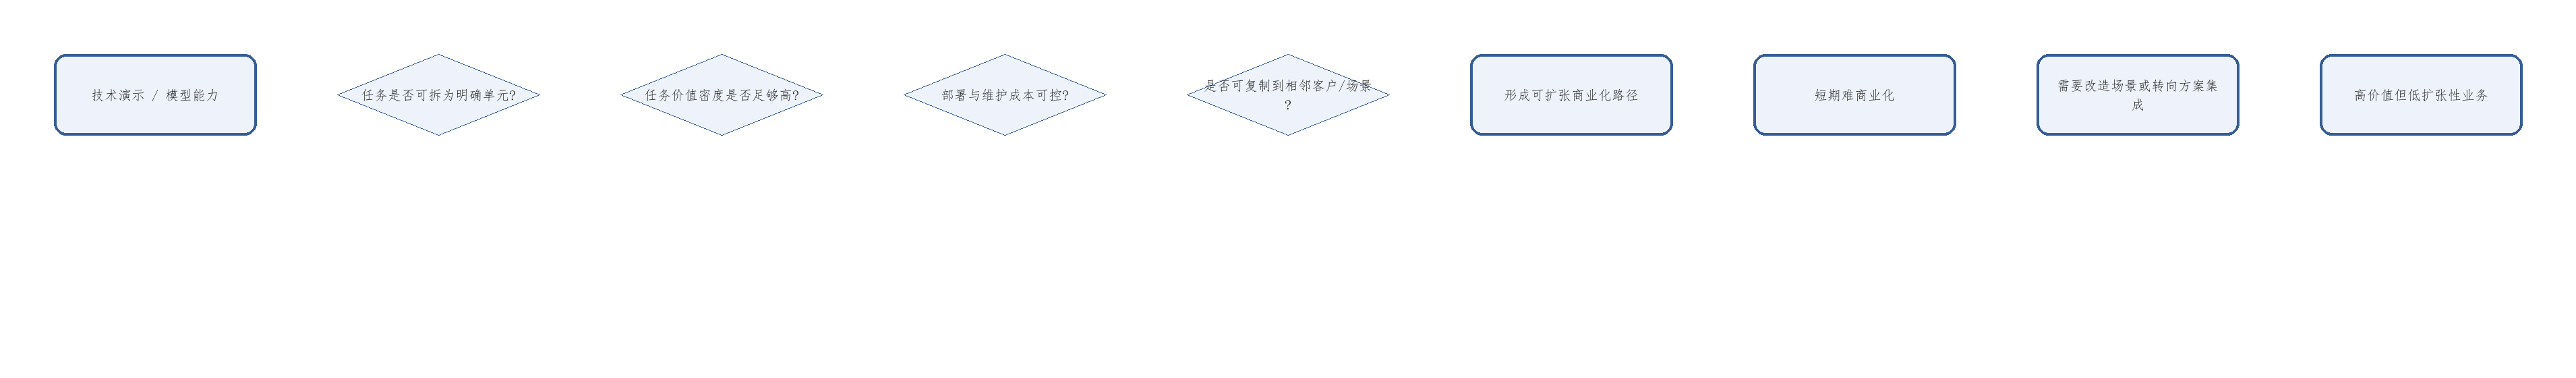
\includegraphics[width=0.9\textwidth,height=0.72\textheight,keepaspectratio]{figures/23-商业化筛选流程图.png}
\caption{23-商业化筛选流程图}
\label{fig:23-商业化筛选流程图}
\end{figure}

\chapter*{表 23-1 典型场景任务单元对照表}
\addcontentsline{toc}{chapter}{表 23-1 典型场景任务单元对照表}
\markboth{表 23-1 典型场景任务单元对照表}{表 23-1 典型场景任务单元对照表}

\begingroup
\small
\begin{xltabular}{\textwidth}{YYYYYYY}
\toprule
场景 & 典型任务单元 & 结构化程度 & 误差容忍度 & 维护难度 & 监管强度 & ROI 可见性 \\
\midrule
\endfirsthead
\toprule
场景 & 典型任务单元 & 结构化程度 & 误差容忍度 & 维护难度 & 监管强度 & ROI 可见性 \\
\midrule
\endhead
制造 & 上下料、工位协作、质检 & 高 & 中 & 中 & 中 & 高 \\
仓储物流 & 分拣、搬运、补货、拣选 & 高 & 中 & 中 & 中 & 高 \\
巡检 & 楼宇/电力/园区巡检 & 中高 & 中 & 中 & 中 & 中高 \\
农业 & 采摘、喷洒、巡田 & 中 & 中 & 高 & 中 & 中 \\
家庭服务 & 收纳、清洁、照护辅助 & 低 & 低 & 高 & 中高 & 低到中 \\
医疗康复 & 辅助操作、康复训练、转运 & 中 & 低 & 高 & 高 & 中 \\
\bottomrule
\end{xltabular}
\endgroup

\chapter*{图表与案例补充}
\addcontentsline{toc}{chapter}{图表与案例补充}
\markboth{图表与案例补充}{图表与案例补充}

本章的图表与案例补充，最重要的不是把场景列得更多，而是把“任务单元 - 约束条件 - 自动化边界 - 商业模式适配”之间的关系固定下来。这样后续新增场景时，就可以直接判断它究竟更接近制造、物流、家庭服务还是高风险环境，而不是每次重新发明一套分类语言。

在长期版本维护中，这一章尤其适合沉淀三类案例。第一类是“先在狭窄场景成功，再逐步扩边界”的正例；第二类是“演示很强但单位经济性始终不闭合”的反例；第三类是“通过人在回路或远程接管先形成业务，再逐步提高自主度”的过渡型案例。只有三类案例并列，商业化章节才不会被单边叙事带偏。

应用落地章节中的图表补充，核心目标是把“商业化判断”从泛泛叙事变成结构化筛选。对具身智能而言，真正决定一个场景能否先跑通的，往往不是展示是否震撼，而是任务结构化程度、误差后果、维护负担和价值密度是否同时满足部署条件。

因此，本章图表不应只是总结性的可视化，而应服务于一个更实用的问题：面对一个新场景时，研究者或分析者应怎样快速判断它更接近“值得进入的商业入口”，还是“更适合作为长期研发目标”。这也是后续版本继续增补行业案例时最值得复用的分析骨架。

在当前版本中，\texttt{\detokenize{图 23-1 商业化筛选流程图}} 已承担“从能力演示到可复制部署”的主流程表达；\texttt{\detokenize{表 23-1 典型场景任务单元对照表}} 则把制造、仓储、巡检、农业、家庭、医疗等场景的误差容忍度、维护难度、监管强度与 ROI 可见性放入统一比较口径。

“值不值得先做”的问题，最终需要被转译成半结构化的 ROI 判断，而不是只停留在定性描述上。23-场景ROI粗估模板 的作用，正是在“人工成本替代、部署改造成本、维护负担、责任风险和复制难度”之间建立统一口径，使场景优先级讨论具备跨版本可更新性。

后续如果要把这一章真正用作季度判断工具，建议同时配合 23-典型场景任务单元对照表 和 23-场景ROI粗估模板 使用。前者负责拆任务单元，后者负责把“值不值得先做”写成统一粗估口径。

若后续更偏向结构化维护，则可以优先使用 23-场景ROI粗估模板-脚本生成版。这样场景字段可以先在 \path{data/processed/场景ROI粗估模板-v0.0.csv} 中修改，再统一导出，避免正文表格和底层字段长期分叉。

\input{chapters/24-产业格局、资本与政策}
\input{chapters/25-关键争议与作者判断框架}
\input{chapters/26-结论与后续跟踪清单}
% Generated from 27-兴趣议题编录与延伸研究.md; edit the LaTeX source after migration.

\reportpart{第二十七部分 兴趣议题编录与延伸研究}
\addcontentsline{toc}{part}{第二十七部分 兴趣议题编录与延伸研究}
\markboth{第二十七部分 兴趣议题编录与延伸研究}{第二十七部分 兴趣议题编录与延伸研究}

本部分不承担“重新概括全书”的职责，而是专门为那些具有长期研究价值、但又不适合完全塞回主线章节的议题保留正式位置。这样做有两个直接好处。第一，主线正文可以继续围绕“问题定义 - 技术主线 - 工程约束 - 产业判断”推进，而不必因为个别兴趣议题不断膨胀。第二，像 RoboCup、多模态编码逻辑这类问题，后续很可能随着论文、规则和工程路线持续演化，单独成章更利于逐版本追踪。

\section*{120. 为什么保留“兴趣议题编录”}
\addcontentsline{toc}{chapter}{120. 为什么保留“兴趣议题编录”}
\markboth{120. 为什么保留“兴趣议题编录”}{120. 为什么保留“兴趣议题编录”}

\subsection*{120.1 它与主线正文的关系}
\addcontentsline{toc}{section}{120.1 它与主线正文的关系}


这份报告的主线正文强调的是“建立判断框架”，因此必须优先保证结构稳定、概念清晰、接口明确。相比之下，兴趣议题往往有两个特征：一是它们不一定在当前行业主线上占最大篇幅，但对长期理解很重要；二是它们常常横跨多个章节，例如既涉及基础模型，也涉及机器人竞赛、教育训练、评测制度或系统工程文化。若强行把这类问题完全摊薄到各章里，读者会很难形成连续认知。

因此，本部分更像“专题档案室”而不是“附录杂项”。它不是把边角料堆在最后，而是把那些值得长期单独追踪的问题正式升级为报告结构的一部分。这样处理之后，主线章节可以维持清晰的职责分工，而专题讨论则可以保留更强的纵深与延展性。

更进一步说，本章承担的是“主线章节之间的回调缓冲层”职责。像 RoboCup 这样的话题，会同时牵引 \texttt{\detokenize{05-控制与状态估计}}、\texttt{\detokenize{06-学习闭环}}、\texttt{\detokenize{12-规划与决策}}、\texttt{\detokenize{14-评测基础设施}} 与 \texttt{\detokenize{17-学术前沿}}；多模态编码逻辑则会同时牵引 \texttt{\detokenize{07-大模型基础}}、\texttt{\detokenize{08-系统架构与分层接口}}、\texttt{\detokenize{11-VLA}} 与 \texttt{\detokenize{13-数据工程}}。若把这些内容平均摊回各章，读者看到的只会是若干分散片段；而把它们保留在同一专题里，反而更容易看清它究竟如何跨章节地改变判断口径。

若把一个兴趣议题是否值得保留写成一个更稳定的判断式，可以粗略表示为：

\begingroup
\scriptsize
\begin{equation*}
\text{Topic Priority} \approx w_1 \cdot \text{cross-chapter pull} + w_2 \cdot \text{evidence flow} + w_3 \cdot \text{judgment impact},
\end{equation*}
\endgroup

其中 \texttt{\detokenize{cross-chapter pull}} 表示该议题是否稳定牵引多个主线章节，\texttt{\detokenize{evidence flow}} 表示近一到两年是否有持续、公开、可复查的新证据流，\texttt{\detokenize{judgment impact}} 表示它是否足以回调全书的既有判断。只有这三个量至少有两个持续为高，本章中的专题位置才是合理的；否则，它更适合降级到 \path{research/} 下的研究资产，而不必长期占据正式正文。

\subsection*{120.2 它与长期跟踪卡片/论文卡的关系}
\addcontentsline{toc}{section}{120.2 它与长期跟踪卡片/论文卡的关系}


兴趣议题编录的另一个作用，是为 \path{research/} 下的长期资产提供上位索引。主线正文通常负责形成阶段性判断，但后续真正驱动版本更新的，往往是论文卡、企业卡、规则更新记录、benchmark 跟踪卡和季度事件日志。本部分正好可以充当这些资产的“阅读入口”：当某个议题后续积累了更多论文、规则或案例时，不必重写主线全书，而是优先回写对应专题，再评估是否需要触发主线章节回调。

也就是说，本部分并不是正文之外的松散笔记，而是“正文判断”和“结构化研究资产”之间的中间层。对长期版本维护来说，这一层非常重要，因为它能显著降低每次更新时的上下文重建成本。

对本项目而言，一个成熟的兴趣议题，最好同时拥有四层资产：

\begin{enumerate}
\item 正文专题：位于本章，用于陈述阶段性判断和与主线的关系。
\item 研究底稿：位于 \path{research/notes/}，用于沉淀资料清单、问题定义、路线分歧与下一轮研究入口。
\item 结构化卡片：位于 \path{research/papers/}、\path{research/companies/} 或后续新增的规则/benchmark 目录中，用于长期积累一手证据。
\item 回调记录：位于 \path{docs/planning/current/当前版本工作台.md}，用于记录“何时因该专题触发正文回写”。
\end{enumerate}

例如，RoboCup 专题不应只在本章存在，还应同时挂接 27-兴趣议题编录与延伸研究-研究底稿 中的赛道与论文清单；多模态编码逻辑专题则不应只停留在正文论证里，还应持续回写到相关论文卡、实验问题清单与 \path{07/08/11/13} 的技术判断上。只有这样，专题才不会变成一次性长文，而会真正变成跨版本可维护的知识索引。

\subsection*{120.3 如何把这里的问题转化为后续版本更新任务}
\addcontentsline{toc}{section}{120.3 如何把这里的问题转化为后续版本更新任务}


一个兴趣议题是否应继续保留，不应只看作者是否主观感兴趣，而应看它是否满足至少一个条件：第一，它持续牵引多个主线章节；第二，它在近期出现稳定的新证据流；第三，它能反过来修正整本报告的判断框架。若某个议题只偶发出现、与主线弱耦合、也缺少连续新证据，那么它更适合被记录在研究卡片里，而不一定继续保留为正式专题。

对后续版本而言，本部分最理想的更新方式不是“越写越长”，而是“越写越结构化”。每次版本迭代时，应优先回答：这个专题新增了哪些一手证据，改变了哪条旧判断，是否触发了其他章节的结构回调。只有这样，本部分才会成为全书长期维护的助推器，而不是尾部膨胀的负担。

更可执行的做法，是把“兴趣议题 -> 更新任务”的转换固定成一个最小流程：

\begin{enumerate}
\item 先记录新增证据：论文、规则变化、官方技术文档、工程案例或 benchmark 更新。
\item 再判断影响范围：它是否只改变专题内部判断，还是已经触发 \texttt{\detokenize{>= 2}} 个主线章节的判断变化。
\item 最后决定回写层级：只更新 \path{research/} 资产、回写本章专题，还是同步回写主线章节与工作清单。
\end{enumerate}

若把这套流程写成伪代码，可粗略表示为：

\begin{lstlisting}[language=python]
def should_callback(topic):
    return topic.new_primary_evidence and (
        topic.touches_mainline_chapters >= 2
        or topic.changes_core_judgment
        or topic.requires_new_tracking_asset
    )
\end{lstlisting}

这段伪代码的意义不是把研究机械化，而是把“何时该动正文、何时只补资产”从主观感觉变成显式规则。对长期维护来说，这一点尤其重要，因为兴趣议题最容易无限膨胀；只有把回写条件固定下来，专题章节才会成为全书的维护加速器，而不是新的上下文负担。

\section*{121. RoboCup：从机器人竞赛到具身系统试验场}
\addcontentsline{toc}{chapter}{121. RoboCup：从机器人竞赛到具身系统试验场}
\markboth{121. RoboCup：从机器人竞赛到具身系统试验场}{121. RoboCup：从机器人竞赛到具身系统试验场}

\subsection*{121.1 赛道、规则与能力维度再编录}
\addcontentsline{toc}{section}{121.1 赛道、规则与能力维度再编录}


从主线正文回到 RoboCup，可以更明确地看到它为何值得被单列。它不是一个单纯的“学术活动信息源”，而是一套把具身能力拆分成多个压力测试场的制度。足球赛道强调动态对抗、多体协同、实时闭环与本体约束；家庭服务赛道强调交互、服务流程与家庭环境中的任务组织；救援赛道强调恶劣环境中的移动、感知与可靠性；工业赛道则把装配、物流、节拍、流程衔接与工艺约束显式拉回研究中心。可参见\href{https://www.robocup.org/domains/1}{RoboCup Soccer 官方页}、\href{https://athome.robocup.org/}{RoboCup@Home 官方页}和\href{https://www.robocup.org/domains/2}{RoboCup Rescue 官方页}。

从能力维度看，RoboCup 的真正价值在于它很少只考一个模块。哪怕是看似“最偏算法”的赛道，也往往会把感知、控制、任务切换、异常恢复和团队协作捆绑在一起。因此，它更接近“系统组织能力考场”，而不是单点模型指标榜。这一点与当前许多静态 benchmark 有根本不同。

如果把它写成一条更适合后续版本更新的判断规则，那么 RoboCup 值得长期保留，恰恰因为它同时满足三件事：第一，它牵引主线正文里的控制、状态估计、规划、学习、评测与部署多个章节；第二，它每年都有可公开追踪的规则变化、赛道变化和团队系统论文；第三，它天然能对“具身能力到底是 demo，还是系统性能力”提出反向追问。具备这三条性质的话题，在整本报告里并不多，因此它值得保留为尾声专题，而不是零散埋进各章。

若进一步按本体形态和技术栈拆开看，RoboCup 的信息量其实比“足球比赛”这个表面印象大得多。不同赛道对应的是不同系统难题：

\begin{enumerate}
\item \texttt{\detokenize{Soccer}} 赛道覆盖标准平台、仿真、多足/轮式中型平台、人形等不同本体约束，难点从视觉定位、队形协作、嵌入式实时通信一路延伸到步态控制、摔倒恢复和高速对抗下的局部重规划。
\item \texttt{\detokenize{@Home}} 更像“家庭服务系统测试场”，常用移动底盘、机械臂、麦克风阵列和语音/视觉交互模块，重点考查任务分解、语义理解、导航与服务流程组织。
\item \texttt{\detokenize{Rescue}} 把不确定地形、受限感知、鲁棒通信和人机协同放在前台。
\item \texttt{\detokenize{Industrial}} 相关赛道则更强调工位节拍、物料流、装配精度、异常恢复和流程对接。
\end{enumerate}

也就是说，RoboCup 的真正价值并不在于某一赛道有多炫，而在于它把“不同本体形态对应什么样的系统难题”组织成了可持续比较的公开制度。

\subsection*{121.2 传统技术栈与新具身路线的交叉评议}
\addcontentsline{toc}{section}{121.2 传统技术栈与新具身路线的交叉评议}


RoboCup 对今天最重要的启发，不是简单证明“传统方法落后、学习方法先进”，而是逼迫我们更精细地讨论二者边界。过去的人形足球确实大量依赖传统步态控制、视觉定位、有限状态机和局部手工调参；但这些方法之所以长期存在，并不是因为研究者不想学习化，而是因为它们在高频闭环、有限算力和强实时约束下具有清晰、可验证、可调试的优势。

今天的新变化，是学习方法开始在局部模块中逐步侵入：感知更具开放性，动作技能可通过示教、仿真和蒸馏获得更强适应性，多模态输入也开始被重新组织进策略网络之中。\href{https://arxiv.org/abs/2504.20808}{SoccerDiffusion 论文}和\href{https://arxiv.org/abs/2602.05310}{渐进式感知-动作人形足球技能论文}都属于这一趋势。但反过来说，RoboCup 也持续证明：只靠更“智能”的高层接口，而不解决定位、平衡、恢复、时延和系统调度问题，并不能让机器人突然踢好一场球。

因此，我更倾向把 RoboCup 看成一个非常好的“反幻觉装置”。它能持续提醒读者：具身能力的提升往往来自大量局部环节的同时改进，而不是来自单一宏大模型叙事。对今天的大模型路线而言，这种提醒尤其宝贵。

从后续版本维护角度，这个专题最值得持续追的不是“哪支队伍夺冠”，而是以下四类信号：

\begin{enumerate}
\item 规则变化是否把任务重心从静态技能进一步推向动态协同、全场自主与异常恢复。
\item 强队系统论文中，学习方法究竟进入了哪些层级：感知层、局部技能层、高层策略层，还是只是参数调优层。
\item 仿真训练、数据回流和嵌入式部署之间是否出现了更稳定的工程闭环。
\item RoboCup 赛道中的能力，是否开始被更明确地迁移到家庭服务、移动操作、工业装配或搜救场景。
\end{enumerate}

只有围绕这四类信号持续更新，这个专题才真正服务于长期研究，而不是停留在“有趣但不影响主线判断”的层面。

\subsection*{121.3 对学术训练、工程教育与现实落地的启发}
\addcontentsline{toc}{section}{121.3 对学术训练、工程教育与现实落地的启发}


RoboCup 最大的非论文价值，在于它为机器人研究提供了一种稀缺的训练方式：研究者必须学会让系统长期运行、现场恢复、多人协同、遵守规则、面对对手与扰动，并在公开环境中接受失败。这类训练在实验室离线 benchmark 中很难获得，但对真实机器人系统至关重要。

对现实落地而言，RoboCup 的启发不是“企业应照搬比赛任务”，而是“企业和研究团队都应重视这种系统级压力测试文化”。真正可部署的具身系统，需要的不是一次惊艳演示，而是在扰动、时延、局部错误和长期运行中依然能维持组织性。RoboCup 所锻炼出的，正是这种能力。

因此，后续版本若继续维护这个专题，最合适的更新方式不是简单加长叙述，而是按以下模板回写：今年最关键的规则变化是什么；哪些团队把学习路线真正推进到了新层级；哪些能力仍然长期依赖传统模块式系统；这些变化是否足以回调主线正文中的某条旧判断。只要坚持这个模板，RoboCup 专题就能持续成为全书的“现实检验入口”。

对工程教育而言，RoboCup 还有一个经常被忽略的价值：它迫使团队同时训练“算法能力”和“运行能力”。一个能在论文里成立的模块，到了现场还必须面对电池衰减、网络抖动、传感器漂移、碰撞保护、裁判规则、队友状态同步和临场维护，这些因素共同决定系统是否真的可用。也正因如此，RoboCup 提供的不是单纯的竞赛排名，而是一种非常接近真实交付前压力测试的文化样板。对企业来说，未必需要复刻比赛本身，但完全可以借鉴这种做法，在内部建立更频繁的对抗式测试、异常恢复演练和多模块联调纪律。

\section*{122. 多模态大模型编码逻辑：统一 token 接口的能力、边界与潜在替代路线}
\addcontentsline{toc}{chapter}{122. 多模态大模型编码逻辑：统一 token 接口的能力、边界与潜在替代路线}
\markboth{122. 多模态大模型编码逻辑：统一 token 接口的能力、边界与潜在替代路线}{122. 多模态大模型编码逻辑：统一 token 接口的能力、边界与潜在替代路线}

\subsection*{122.1 “先编码、再串行化、再交给语言主干”是否只是权宜之计}
\addcontentsline{toc}{section}{122.1 “先编码、再串行化、再交给语言主干”是否只是权宜之计}


从当前主流路线看，这种范式几乎可以说是事实上的行业默认接口。无论是 \href{https://arxiv.org/abs/2301.12597}{BLIP-2} 的 Q-Former、\href{https://arxiv.org/abs/2204.14198}{Flamingo} 的 Perceiver Resampler、\href{https://arxiv.org/abs/2304.08485}{LLaVA} 的视觉投影，还是 \href{https://arxiv.org/abs/2303.03378}{PaLM-E} 将连续状态接入语言主干，本质上都在做同一件事：先让模态专用编码器处理原始信号，再把结果映射到语言主干可消费的上下文接口。

所以，如果问“这是不是权宜之计”，更准确的回答是：它既是权宜之计，也是当前最成功的复用范式。它的成功之处在于极大降低了多模态系统的构建门槛，并复用了大语言模型已经具备的强大上下文能力；它的局限之处在于，这种接口天然带有压缩、时延和模态鸿沟问题，尤其在机器人所关心的高频状态与动作连续性上更明显。

把这个判断再压实一点，可以说：这套路线成功的根本原因，不是它完美，而是它把“多模态系统的困难”转写成了一个今天工程界最擅长处理的问题，即如何把不同来源的信息组织进统一上下文接口。它失败的风险则在于，一旦这种转写把本来属于几何、接触、动力学和控制新鲜度的问题伪装成“序列建模问题”，系统就会在表面统一的同时牺牲掉真正难以恢复的物理信息。

因此，这一争论的关键并不是“词元化是否优雅”，而是“哪些信息适合被压成统一上下文，哪些信息根本不该被压成同一种上下文”。对机器人而言，语言目标、任务约束和低频语义提示通常适合被统一处理；但触觉、本体状态、闭环控制新鲜度、动作连续性和高频观测变化，往往更接近“必须保留专用结构”的信息类型。也就是说，串行 token 接口真正面对的，不是抽象的美学问题，而是信息保真度与系统时延预算的分配问题。

\subsection*{122.2 主流改良路线：更强连接器、token 压缩、latent 接口与原生多模态趋势}
\addcontentsline{toc}{section}{122.2 主流改良路线：更强连接器、token 压缩、latent 接口与原生多模态趋势}


学界对这一路线的反思，并没有停留在“抱怨词元化不好”，而是已经沿若干明确方向展开改良。第一类是更强连接器，例如 Q-Former、重采样器和各类潜变量查询结构，它们试图在固定预算下让接口保留更多任务相关信息，\href{https://arxiv.org/abs/2301.12597}{BLIP-2}和\href{https://arxiv.org/abs/2107.14795}{Perceiver IO 论文}代表了这一路线。第二类是词元压缩与裁剪，围绕上下文预算与视觉冗余进行主动筛选，代表工作包括\href{https://arxiv.org/abs/2504.09897}{TAMP 论文}、\href{https://arxiv.org/abs/2503.10501}{TokenCarve 论文}和\href{https://arxiv.org/abs/2506.01097}{通用词元压缩论文}。

第三类是显式处理模态鸿沟与接口失配，而不是假设对齐天然会发生。\href{https://arxiv.org/abs/2203.02053}{模态鸿沟论文 Mind the Gap}和\href{https://arxiv.org/abs/2602.07026}{ReAlign 论文}都表明，多模态表示之间的几何偏差与任务偏差是真实存在的，需要被单独建模。第四类趋势则更“激进”：减少对纯语言主干的依赖，转向更原生的多模态主干、并行潜变量状态、专用动作通路和多时间尺度接口。这些路线未必已经收敛成统一范式，但它们至少说明，社区并不满足于永远把所有模态都塞进同一串序列里。

如果进一步从“替代串行词元接口”的角度理解这些路线，它们大致在回答两类问题。第一类问题是“还能不能继续沿统一上下文范式优化”，对应更强连接器、预算分配器和词元压缩器；第二类问题是“哪些信息根本不该完全进入同一串序列”，对应并行潜变量状态、专用状态/动作旁路、多时间尺度控制接口等做法。前者是在修补现有主干，后者则是在局部拒绝“所有信息都应被同一种序列接口消费”的假设。对具身系统来说，真正值得长期关注的往往恰恰是后者，因为机器人最敏感的信号正是那些最容易在统一接口中被抹平的信号。

从工程上看，这几类改良路线还对应着完全不同的能力边界。更强连接器和 token 压缩，本质上是在“固定主干 + 固定预算”约束下改进信息挑选方式，因此它们通常最适合提升多模态理解效率；latent 接口、状态旁路和多时间尺度架构，则是在重新划分“谁负责语义，谁负责几何，谁负责高频控制”。对具身系统而言，后者往往更接近真正的结构性改良，因为它直接回应了机器人最核心的两个现实约束：控制新鲜度和物理信息保真。未来若某条路线宣称显著改进了多模态机器人能力，本报告最值得优先追问的就是：它到底是在更聪明地压缩 token，还是已经开始重新划分不同信息流应走的接口。

\subsection*{122.3 后续值得跟踪的论文、实验与理论问题}
\addcontentsline{toc}{section}{122.3 后续值得跟踪的论文、实验与理论问题}


围绕这一专题，我认为后续最值得持续跟踪的不是“谁又提出了一个新连接器名字”，而是三个更本质的问题。第一，哪些模态必须保留专用结构，不能被过度串行化。对机器人来说，触觉、力觉、本体状态和高频动作接口尤其关键。第二，哪些能力退化可以通过更强连接器弥补，哪些退化其实源于错误的问题接口定义。第三，学界能否从目前以经验消融为主的证据体系，进一步推进到更清晰的能力边界解释，甚至形成更强的理论约束。

如果这些问题未来获得更明确答案，那么它对具身智能的影响可能不亚于再出现一个更大的通用模型。因为对于机器人而言，很多上限并不只由“主干模型聪不聪明”决定，更由“世界信息是如何被送进主干”的方式决定。也因此，这个专题值得被保留在报告尾声，作为后续版本长期追踪的一条主线问题。

为了让后续版本真正可执行，我建议把这一专题的追踪任务固定成三组：

\begin{enumerate}
\item 论文组：持续追踪连接器、模态鸿沟修正、token 压缩、动作接口和原生多模态主干五类论文，而不是只追单一热门模型名词。
\item 实验组：重点看预算-性能曲线、不同模态删减实验、动作频率变化实验、状态旁路有无对照实验，而不是只看单一 benchmark 分数。
\item 理论组：持续追踪是否出现更清晰的“哪些信号必须保留专用结构、哪些信号可安全串行化”的解释框架。
\end{enumerate}

这三组任务之所以重要，是因为它们直接决定未来版本能否回答一个更难但也更有价值的问题：多模态大模型的下一次关键突破，究竟会主要来自更大的主干，还是来自更合理的信息接口设计。

